
 
    
%%%%%%%%%%%%%%%%%%%%%%%%%%%%%%%%%%%%%%%%%%%%%%%%%%%%%%%%%%%%%%%%%%%%%%%%%%%%%%
% ASU Dissertation Template
%%%%%%%%%%%%%%%%%%%%%%%%%%%%%%%%%%%%%%%%%%%%%%%%%%%%%%%%%%%%%%%%%%%%%%%%%%%%%%
% Copyright 2020 Robert W. Kutter (robert@kutterconsulting.com)
%
%   See also: http://kutterconsulting.com
%
% For guidance on using this file, see the README.
%
%%%%%%%%%%%%%%%%%%%%%%%%%%%%%%%%%%%%%%%%%%%%%%%%%%%%%%%%%%%%%%%%%%%%%%%%%%%%%%
% Preamble
%%%%%%%%%%%%%%%%%%%%%%%%%%%%%%%%%%%%%%%%%%%%%%%%%%%%%%%%%%%%%%%%%%%%%%%%%%%%%%
\newcommand*{\pointsize}{12pt}          %<Set the font size; make sure the size is correct
                                        %   for the font you will use
\documentclass[letterpaper,             % Use US letter-size paper
               oneside,                 % No verso and recto differences
               \pointsize]              % Uses the font size defined above
               {memoir}
\renewcommand{\cleardoublepage}%        % \cleardoublepage will create entirely blank
  {\clearpage}%                         %   pages depending on settings (e.g., usually
                                        %   before start of \mainmatter); redefine it here
                                        %   so that no entirely blank pages are created
                                        %   automatically
%%%%%%%%%%%%%%%%%%%%%%%%%%%%%%%%%%%%%%%
% (Some) Packages
%%%%%%%%%%%%%%%%%%%%%%%%%%%%%%%%%%%%%%%

%\usepackage{setspace}   %Allows double spacing with the \doublespacing command

%\usepackage{fontspec}
%\setmainfont{Arial}
\usepackage[Export]{adjustbox} % Used to constrain images to a maximum size
\adjustboxset{max size={0.9\linewidth}{0.9\paperheight}}
\usepackage{array}
\usepackage{afterpage}
\usepackage{amsmath,amssymb,amsbsy}
\usepackage{booktabs}
\usepackage[font=doublespacing,font=footnotesize]{caption}
%\captionsetup{font={large,stretch=1.3}}
\usepackage{comment}
\usepackage{courier}
\usepackage{dcolumn}
\usepackage{enumerate} % Needed for markdown enumerations to work
\usepackage{eurosym} % defines \euro
\usepackage{fancyhdr}
\usepackage{fancyvrb} % verbatim replacement that allows latex
\usepackage{float}
\floatplacement{figure}{H} % forces figures to be placed at the correct location
\usepackage{geometry}
\usepackage{tocloft}
%\usepackage[titles]{tocloft}%
\usepackage{natbib}
%\usepackage{asudis}
\usepackage{graphicx}
\usepackage{grffile} % extends the file name processing of package graphics 
\usepackage{hyperref}
\usepackage{listings}
\lstset{basicstyle=\footnotesize\ttfamily,breaklines=true}
\lstset{framextopmargin=0pt,frame=single}
\usepackage{longtable}
\usepackage{minted}

%\usepackage{sectsty}
%\usepackage{setspace}
\usepackage{siunitx}
\usepackage{tcolorbox}
\usepackage{textcomp} % defines textquotesingle

\usepackage[mathletters]{ucs} % Extended unicode (utf-8) support
\usepackage{upquote} % Upright quotes for verbatim code
\usepackage{xcolor} % Allow colors to be defined


\usepackage{graphicx}                   % For importing image files
\usepackage{etoolbox}                   % For advanced commands throughout preamble
\usepackage{minted}
\usepackage{microtype}                  %~Improves kerning and protrusion (optional);
                                        %   See here for an introduction:
                                        %   http://www.khirevich.com/latex/microtype/

\providetoggle{usemicrotype}            % TRUE = microtype is being used
\makeatletter                           %   (Used to turn of microtype protrusion in the
\@ifpackageloaded{microtype}%           %   table of contents.)
  {\settoggle{usemicrotype}{true}}%
  {\settoggle{usemicrotype}{false}}
\makeatother
\usepackage{changepage}                 % For changing page layout (e.g., margins) in the
                                        %   middle of the document
\usepackage{calc}					              % Calculate text widths; used in page layout
                                        %   changes

%%%%%%%%%%%%%%%%%%%%%%%%%%%%%%%%%%%%%%%
% Title page, input
%%%%%%%%%%%%%%%%%%%%%%%%%%%%%%%%%%%%%%%
\listadd{\titlelines}%
  {Neuronal Deep Fakes}             %<Enter the title of the dissertation
\listadd{\titlelines}%
  {Data Driven Optimization of Reduced Neuronal Models}            % If you want to
                                        %   split the title across lines,
                                        %   use another \listadd command for the
                                        %   second line
\newcommand*\Author{Russell J Jarvis}          %<Enter your name; must match official transcript
\newcommand*{\documentname}%
  {Dissertation}                        %<Enter the type of document (capitalized)
\newcommand*{\degreename}
  {Doctor of Philosophy}                %<Enter the type of degree (capitalized)
\newcommand*\defdate{November 2020}        %<Give month (written out fully) and year of
                                        %   the oral defense
%\listadd{\committeechair}{Chair Name}   %<Enter committee chair name; use \listadd for
%\listadd{\committeechair}{Another name}%   for additional names
%\newcommand*{\chairlabel}{Co-Chair Sharon M. Crook}        %<If you have co-chairs, replace this text with
%\newcommand*{\committeemember}{Co-Chair Rick Gerkin}        %<If you have co-chairs, replace this text with        \memberOne{Sharon Crook, Co-Chair}
%\memberOne{}
                          %   'Co-Chair'
%\listadd{\committeemember}{Yi Zhou} %<Enter committee member names; use \listadd for
%\listadd{\committeemember}{James J Abbas} %   additional names
%\newcommand*{\gradmonth}{November}         %<Enter the graduation date; month can only be:
                                        %  May, August, or December
%\newcommand*{\gradyear}{2020}           %<Enter the graduation year, e.g. 2014

\listadd{\keywords}{genetic algorithms}          %<Enter keywords; use \listadd for
\listadd{\keywords}{optimisation}         

\newcommand{\gradmonth}{December}
\newcommand{\gradyear}{2020}

%   additional names (up to 6)
\newcommand*{\graddate}{\gradmonth   \space\gradyear}



%\title{Neuronal Deep Fakes: Data-Driven Optimization of Reduced Neuronal Models}
%\author{Russell Jarrod Jarvis}
%\degreeName{Doctor of Philosophy}
%\paperType{Dissertation}
%\defensemonth{November}
%\gradmonth{December}
%\gradyear{2020}
%\chair{Sharon Crook, co-Chair}
%\memberOne{Sharon Crook, Co-Chair}
%\memberOne{}
%\memberTwo{Rick Gerkin, Co-Chair}
%\memberThree{Yi Zhou}
%\memberFour{James Abbas}

%%%%%%%%%%%%%%%%%%%%%%%%%%%%%%%%%%%%%%%
% Page layout
%%%%%%%%%%%%%%%%%%%%%%%%%%%%%%%%%%%%%%%
\settrimmedsize{\stockheight}%          % Specifies \paperheight and \paperwidth
  {\stockwidth}{*}
\settrims{0pt}{0pt}                     % Set location of page in relation to the stock.
                                        % Paper and stock size are equivalent,
                                        % so both \trimtop and \trimedge are set to 0pt
\newlength{\forfootskip}
\setlength{\forfootskip}%
  {3\baselineskip}
\newlength{\textblockheight}            % Calculate height of text block to leave room
\setlength{\textblockheight}{9.0in}     %   for footers, keeping page numbers outside
\addtolength{\textblockheight}%         %   the 1in vertical margins
  {-\forfootskip}
\settypeblocksize{\textblockheight}%    % Calculated by 1.0in vertical margins and
  {*}{*}                                %   letting margins set the width of the typeblock
\setulmargins{1.0in}{*}{*}              % Set upper margin (\uppermargin, not \topmargin);
                                        %   calculate the bottom margin
\setlrmarginsandblock{1.25in}{1.25in}{*}%~Set margins and calculate width of typeblock
\setheaderspaces{*}{0.5\baselineskip}{*}% Arguments: '\headdrop', '\headsep', and/or ratio
                                        %   Note: This is only used in the list of
                                        %   contents sections
\setheadfoot{\baselineskip}%            % Set '\headheight' and '\footskip'
  {\forfootskip}
\checkandfixthelayout                   % Required by memoir package after setting layout
\settypeoutlayoutunit{in}               % Write layout dimensions to log file in inches

%%%%%%%%%%%%%%%%%%%%%%%%%%%%%%%%%%%%%%%
% Fonts
%%%%%%%%%%%%%%%%%%%%%%%%%%%%%%%%%%%%%%%
\usepackage[T1]{fontenc}                % Standard option to handle, e.g., accented
                                        %   characters like 'ö' better
\usepackage{amssymb,mathtools}          % For AMS-LaTeX, see here for more:
                                        %     http://www.ams.org/publications/authors/tex/amslatex
                                        % ('mathtools' loads and extends 'amsmath')
\usepackage{ifxetex,ifluatex}           % Can check if XeTeX or LuaTeX was used to typeset
\usepackage{fixltx2e}                   % Provides \textsubscript
\IfFileExists{upquote.sty}%             % Use upquote if available, for
  {\usepackage{upquote}}{}              %   straight quotes in verbatim environments

% Load fonts depending on the
%   typesetting engine
\ifnum 0\ifxetex 1\fi\ifluatex 1\fi=0   % If pdftex
  \usepackage[utf8]{inputenc}           %   'utf8' should match the encoding of this file
                                        %
                                        %~Set up your font in pdftex here
                                        %
\else 									                % If xetex or luatex
  \ifxetex                              % If xetex
    \usepackage{mathspec}               % Matches non-math open-type font to math
                                        %   open-type font (use 'mathspec' if you want to
                                        %   write math in unicode)
    \usepackage{xunicode}               % Convert LaTeX character macros to unicode
  \else                                 % If luatex\usepackage{fontspec}
    \usepackage{fontspec}               % Use fontspec for (open type) font selection
  \fi
  \defaultfontfeatures{Mapping=tex-text,% Font spec setting
    Scale=MatchLowercase}
  \newcommand*{\euro}{€}

  % Using fonts in XeLaTeX can be complicated; the following settings
  % work when this file is compiled inside the Docker container produced
  % by the `build.sh` script.
  %
  % Sometimes something simple like the following will work:
  %
  %   \setmainfont{Garamond}
  %
  % But often the easiest solution is to move font files (*.otf or *.ttf) into
  % a sub-directory and provide the direct path to them here.
  %
  % See `fontspec` documentation for more on using local font files.
  %
  \setmainfont{EBGaramond12}[           %<Set the main font; make sure the font is correct
                                        %   for the font size (See ASU Style Guide)
    Path          = /usr/share/fonts/opentype/ebgaramond/,
    Extension     = .otf ,
    UprightFont   = *-Regular ,
    ItalicFont    = *-Italic ,
    % Notice that bold is missing here because the Docker image does not have
    % a bold typeface for Garamond; it would probably be possible to find
    % one on your local system or online.
  ]

%  \setmathfont(Digits,Latin,Greek)%     %~Uncomment two lines to set a font for math%
%    {MATHFONT}
\fi

%%%%%%%%%%%%%%%%%%%%%%%%%%%%%%%%%%%%%%%
% Line spacing
%%%%%%%%%%%%%%%%%%%%%%%%%%%%%%%%%%%%%%%
\DoubleSpacing                          % True double spacing
\BeforeBeginEnvironment{quote}          % Memoir leaves most special material
  {\par\SingleSpacing}                  %   single spaced, but makes block quotes
\AfterEndEnvironment{quote}%            %   double-spaced; fix to follow ASU style guide
  {\vspace{-\baselineskip} %
  \DoubleSpacing}
\BeforeBeginEnvironment{quotation}%
  {\par\SingleSpacing}
\AfterEndEnvironment{quotation}%
  {\vspace{-\baselineskip} %
  \DoubleSpacing}

\setlength{\footnotesep}{\baselineskip} % Double space *between* footnotes
\renewcommand*{\footnoterule}{%         % Redefine footnoterule so that initial footnote
  \kern-3pt%                            %   still appears right under the rule (changing
  \hrule width 0.4\columnwidth          %   \footnotesep also changes the space between the
  \kern 2.6pt                           %   rule and the first footnote
  \vspace{-0.5\baselineskip}            % (Here is the vertical space adjustment)
  }

\usepackage{enumitem}                   % Control spacing in enumerate environment
\setlist{noitemsep}                     % Remove extra vertical spacing between items in lists
                                        % \setlist{nosep} to leave no space around whole list

%%%%%%%%%%%%%%%%%%%%%%%%%%%%%%%%%%%%%%%
% Page numbering
%%%%%%%%%%%%%%%%%%%%%%%%%%%%%%%%%%%%%%%
\makepagestyle{ASU}
  \makeevenfoot{ASU}{}{\thepage}{}
  \makeoddfoot{ASU}{}{\thepage}{}

%%%%%%%%%%%%%%%%%%%%%%%%%%%%%%%%%%%%%%%
% Title page, formatting
%%%%%%%%%%%%%%%%%%%%%%%%%%%%%%%%%%%%%%%
\newlength{\savedfootskip}
\setlength{\savedfootskip}{\footskip}
\newcommand{\titlepagesetup}{%          % Page layout for title page
  \changepage%                          % Adjustment to page dimensions:
    {\savedfootskip}%                   %   text height
    {}%                                 %   text width
    {}%                                 %   even-side margin
    {}%                                 %   odd-side margin
    {}%                                 %   column sep.
    {}%                                 %   topmargin
    {}%                                 %   headheight
    {}%                                 %   headsep
    {-\savedfootskip}%                  %   footskip
}

\newcommand{\closetitlepagesetup}{%     % Undo set up for title page
  \changepage{-\savedfootskip}{}{}{}{}%
    {}{}{}{\savedfootskip}%
}

\makeatletter                           % Do not modify this section; Enter info above
\newcommand*{\titlepageASU}{
  \titlepagesetup
  \clearpage
  \begin{center}
  \SingleSpacing
  \thispagestyle{empty}
    \renewcommand*{\do}[1]{##1 \\[\baselineskip]}
    \dolistloop{\titlelines}
    by \\[\baselineskip]
    \Author \\[4\baselineskip]
    A \documentname~Presented in Partial Fulfillment \\
    of the Requirements for the Degree \\
    \degreename \\
    \vfill                              % Vertically center the portion below
    Approved \defdate~by the \\
    Graduate Supervisory Committee: \\[\baselineskip]
    %\renewcommand*{\do}[1]{##1, \chairlabel \\}
    %\dolistloop{\committeechair}
    %\renewcommand*{\do}[1]{##1 \\}
    %\dolistloop{\committeemember}
    \memberOne{Sharon M Crook, Co-Chair}\\
    \memberTwo{Rick C Gerkin, Co-Chair}\\
    \memberThree{Yi Zhou}\\
    \memberFour{James J Abbas}\\
    \vfill        
    
    % Vertically center the portion above
    ARIZONA STATE UNIVERSITY \\[\baselineskip]
    \graddate
  \end{center}
  \clearpage
  \closetitlepagesetup
}
\makeatother

%%%%%%%%%%%%%%%%%%%%%%%%%%%%%%%%%%%%%%%
% Heading styles
%%%%%%%%%%%%%%%%%%%%%%%%%%%%%%%%%%%%%%%
% Note: memoir also has \book and \part commands; do not use these
\makechapterstyle{ASU}{%                % Define chapter heading style
  \renewcommand*{\chapterheadstart}{}   % Chapter title flush with top margin
  \renewcommand*{\chapnamefont}%        % Set font for 'Chapter' or 'Appendix'
    {\normalfont}
  \renewcommand*{\chapnumfont}%         % Set font for number in chapter headings
    {\normalfont}
  \renewcommand*{\afterchapternum}%     % Insert a double line break after
    {\\[\baselineskip]}                 %   chapter number
  \renewcommand*{\chaptitlefont}%       % Set font for chapter title name
    {\normalfont}
  \setlength{\afterchapskip}{0pt}       % Set vertical space between chapter title and
                                        %   first paragraph; equivalent to one line break
                                        %   (vertical space = \afterchapskip + \baselineskip)
                                        % Note: This \afterchapskip value is only used in
                                        %   front matter
  \renewcommand*{\printchapternum}{%    % Center justify chapter number
    \centering \chapnumfont %
    \thechapter}
  \renewcommand*{\printchaptertitle}[1]%% Center justify
    {\expandafter\centering %           %   \MakeUppercase has issues; see here for some
    \expandafter\chaptitlefont %        %   details: https://tex.stackexchange.com/questions/35680/uppercase-in-newcommand
    \expandafter\MakeUppercase %        %   Accented characters and some fonts may not
    \expandafter{##1}}                  %   uppercase correctly; if that happens, just
                                        %   type the chapter title in uppercase
}

\setsecnumdepth{all}                    %~Enter the levels that you want to have numbered
                                        %   (Default is to number all [5 levels deep].)

\newcommand{\divisionbeforeskip}%       % Create default formatting for headings
  {\baselineskip}
\newcommand{\divisionindent}%
  {0.5em}
\newcommand{\divisionfont}{\normalfont} % Font must be \normalfont
\newcommand{\divisionafterskip}%
  {\baselineskip}

\setbeforesecskip{\divisionbeforeskip}  % Apply default formatting to all heading levels
\setsecindent{\divisionindent}          % Note: If you change \setsecnumdepth above, you
\setsecheadstyle{\divisionfont}         %   will need to set the indent for all lower
\setaftersecskip{\divisionafterskip}    %   levels to '0pt'; otherwise, they will be
                                        %   preceded by unnecessary space
\setbeforesubsecskip{\divisionbeforeskip}
\setsubsecindent{\divisionindent}
\setsubsecheadstyle{\divisionfont}
\setaftersubsecskip{\divisionafterskip}

\setbeforesubsubsecskip{\divisionbeforeskip}
\setsubsubsecindent{\divisionindent}
\setsubsubsecheadstyle{\divisionfont}
\setaftersubsubsecskip{\divisionafterskip}

\setbeforeparaskip{\divisionbeforeskip}
\setparaindent{\divisionindent}
\setparaheadstyle{\divisionfont}
\setafterparaskip{\divisionafterskip}

\setbeforesubparaskip{\divisionbeforeskip}
\setsubparaindent{\divisionindent}
\setsubparaheadstyle{\divisionfont}
\setaftersubparaskip{\divisionafterskip}

%%%%%%%%%%%%%%%%%%%%%%%%%%%%%%%%%%%%%%%
% Paragraph formatting
%%%%%%%%%%%%%%%%%%%%%%%%%%%%%%%%%%%%%%%
%\sloppybottom                          % Reduce the chances of widows
\raggedbottom                           % Loosens vertical spacing requirements, so
                                        %   \sloppybottom doesn't make pages look bad;
                                        %   it also prevents large gaps in the middle of
                                        %   pages and pushes them to the bottom of pages
\indentafterchapter                     % Overrides the default which is not to indent
                                        %   the first paragraph in a chapter, but it
                                        %   looks odd in some places to not indent
                                        %   paragraphs

%%% List Titles %%%
\renewcommand{\contentsname}%           % Set heading for each list
  {Table of Contents}%                  %   Formatted as chapter headings by default, so
\renewcommand{\listtablename}%          %   no additional heading formatting is needed
  {List of Tables}
\renewcommand{\listfigurename}%
  {List of Figures}

%%% Depth %%%
\settocdepth{subparagraph}              % Include 5 levels deep (all levels) in TOC

%%% Fonts %%%
\makeatletter%
\patchcmd{\l@part}%                     % Patch the command that writes part-level entries
    {\cftpartfont {#1}}%                %   to the table of contents, so they are in
    {\normalfont \texorpdfstring{%      %   'normalfont' and uppercase
      \uppercase{#1}}{{#1}} }%
    {\typeout{Success: Patch %
      'l@part' to uppercase %
      part-level headings in the %
      table of contents.}}%
    {\typeout{Fail: Patch %
      'l@part' to uppercase %
      part-level headings in the %
      table of contents.}}%
\makeatother%

\makeatletter%
\patchcmd{\l@chapapp}%                  % Patch the command that writes chapter-level
    {\cftchapterfont {#1}}%             %   entries to the table of contents, so they are
    {\normalfont \texorpdfstring{%      %   in 'normalfont' and uppercase
      \uppercase{#1}}{{#1}} }%
    {\typeout{Success: Patch %
      'l@chapapp' to uppercase %
      part-level headings in the %
      table of contents.}}%
    {\typeout{Fail: Patch %
      'l@chapapp' to uppercase %
      part-level headings in the %
      table of contents.}}%
\makeatother%

% If not using 'hyperref', use the following commands to adjust 'part' and 'chapter'
%   level headings in the TOC
%\renewcommand*{\cftpartfont}%          % Uppercase 'part' and 'chapter' headings
%  {\normalfont\MakeTextUppercase}      % Note: Sending \MakeTextUppercase to the TOC
%\renewcommand*{\cftchapterfont}%       %   conflicts with hyperref and breaks it!
%  {\normalfont\MakeTextUppercase}%

\usepackage{titlecaps}                  % Set up headline style for captions in the
                                        %   lists of tables and figures
                                        % Note: ASU style guide does not provide
                                        %   comprehensive guidelines for headlines, so
                                        %   Chicago style for headline style is used
                                        % Note: Last word in title is not explicitly
                                        %   capitalized; in general, these settings are
                                        %   broadly correct, but captions should be
                                        %   reviewed to ensure they are being capitalized
                                        %   properly
\Resetlcwords
\Addlcwords{a an the}                   % Leave articles lowercase
\Addlcwords{and but for or nor}         % Leave conjunctions lowercase
\Addlcwords{aboard about above across % % Leave all prepositions lowercase
  after against along amid among anti % %   (This is a [non-exhaustive] list of common
  around as at before behind below %    %   one-word prepositions)
  beneath beside besides between %
  beyond but by concerning considering %
  despite down during except excepting %
  excluding following for from in %
  inside into like minus near of off %
  on onto opposite outside over past %
  per plus regarding round save since %
  than through to toward towards under %
  underneath unlike until up upon %
  versus vs via with within without}
\Addlcwords{ according\space{to} %      % Leave two-word conjunctions lowercase
  ahead\space{of} apart\space{from} %   %   (This is a [non-exhaustive] list of common
  as\space{for} as\space{of} %          %   two-word prepositions.)
  as\space{per} as\space{regards} %
  aside\space{from} astern\space{of} %
  back\space{to} because\space{of} %
  close\space{to} due\space{to} %
  except\space{for} far\space{from} %
  in\space{to} inside\space{of} %
  instead\space{of} left\space{of} %
  near\space{to} next\space{to} %
  on\space{to} opposite\space{of} %
  opposite\space{to} out\space{from} %
  out\space{of} outside\space{of} %
  owing\space{to} prior\space{to} %
  pursuant\space{to} rather\space{than} %
  regardless\space{of} right\space{of} %
  subsequent\space{to} such\space{as} %
  thanks\space{to} that\space{of} %
  up\space{to}}

\renewcommand{\cfttableaftersnumb}%     % Put table captions in List of Tables in title
  {\titlecap}%                          %   case
\renewcommand{\cftfigureaftersnumb}%    % Put table captions in List of Figures in title
  {\titlecap}%                          %   case

\renewcommand*{\cftpartpagefont}%       % Use normal font for all page numbers
  {\normalfont}
\renewcommand*{\cftchapterpagefont}%
  {\normalfont}
\renewcommand*{\cftsectionpagefont}%
  {\normalfont}
\renewcommand*{\cftsubsectionpagefont}%
  {\normalfont}
\renewcommand*{\cftsubsubsectionpagefont}%
  {\normalfont}
\renewcommand*{\cftsubsubsectionpagefont}%
  {\normalfont}
\renewcommand*{\cftparagraphpagefont}%
  {\normalfont}
\renewcommand*{\cftsubparagraphpagefont}%
  {\normalfont}
\renewcommand*{\cftfigurepagefont}%
  {\normalfont}
\renewcommand*{\cfttablepagefont}%
  {\normalfont}

\cftpagenumbersoff{part}                % Turn off page numbers for 'part's, which are
                                        %   actually serving as headings within the TOC

%%% Vertical Space %%%
\setlength{\cftbeforepartskip}{0pt}     % Remove all additional vertical spacing so TOC
\setlength{\cftbeforechapterskip}{0pt}  %   is double spaced uniformly
\setlength{\cftbeforesectionskip}{0pt}
\setlength{\cftbeforesubsectionskip}{0pt}
\setlength{\cftbeforesubsubsectionskip}{0pt}
\setlength{\cftbeforeparagraphskip}{0pt}
\setlength{\cftbeforesubparagraphskip}{0pt}
\setlength{\cftbeforefigureskip}{0pt}
\setlength{\cftbeforetableskip}{0pt}

\renewcommand{\insertchapterspace}{%    % By default, extra vertical space (10pt) is
  \addtocontents{lof}%                  %   inserted between tables and figures from
    {\protect\addvspace{0pt}}%          %   different chapters; remove this extra space.
  \addtocontents{lot}%
    {\protect\addvspace{0pt}}%
  %%
  %
  \addcontentsline{toc}{part}{APPENDIX}
  %
  %%
}

%%% Horizontal Space %%%
\newlength{\levelindentincrement}       % Set indent to increase by the same amount for
\setlength{\levelindentincrement}{2em}  %   each level in the TOC; don't adjust figure
\newlength{\levelindent}                %   or table indents
\setlength{\levelindent}%
  {\levelindentincrement}
\setlength{\cftchapterindent}%
  {\levelindent}
\addtolength{\levelindent}%
  {\levelindentincrement}
\setlength{\cftsectionindent}%
  {\levelindent}
\addtolength{\levelindent}%
  {\levelindentincrement}
\setlength{\cftsubsectionindent}%
  {\levelindent}
\addtolength{\levelindent}%
  {\levelindentincrement}
\setlength{\cftsubsubsectionindent}%
  {\levelindent}
\addtolength{\levelindent}%
  {\levelindentincrement}
\setlength{\cftparagraphindent}%
  {\levelindent}
\addtolength{\levelindent}%
  {\levelindentincrement}
\setlength{\cftsubparagraphindent}%
  {\levelindent}
\addtolength{\levelindent}%
  {\levelindentincrement}

\setlength{\cftchapternumwidth}%        % Decrease space between number and heading for
  {0.85\cftchapternumwidth}             %   all heading levels
\setlength{\cftsectionnumwidth}%
  {0.85\cftsectionnumwidth}
\setlength{\cftsubsectionnumwidth}%
  {0.85\cftsubsectionnumwidth}
\setlength{\cftsubsubsectionnumwidth}%
  {0.85\cftsubsubsectionnumwidth}
\setlength{\cftparagraphnumwidth}%
  {0.85\cftparagraphnumwidth}
\setlength{\cftsubparagraphnumwidth}%
  {0.85\cftsubparagraphnumwidth}

% Calculate the indent to the first
% character in table and figure
% captions.
% This is more complicated because the
% document automatically considers
% the total number of figures and
% tables and increases the indent to
% make room for longer numbers.
\newcounter{totfigures}                 % Collect the total number of figures
\newcounter{tottables}                  % Collect the total number of tables

\providecommand\totfig{}                % Retrieve the total number of figures
\providecommand\tottab{}                % Retrieve the total number of tables

\makeatletter
\AtEndDocument{%                        % Store the totals
  \addtocounter{totfigures}{%
    \value{figure}%
  }%
  \addtocounter{tottables}{%
    \value{table}%
  }%
  \immediate\write\@mainaux{%
    \string\gdef\string\totfig{%
      \number\value{totfigures}%
    }%
    \string\gdef\string\tottab{%
      \number\value{tottables}%
    }%
  }%
}
\makeatother

% The calculation that appears inside
% this block needs to be done as the
% the document is written, not in the
% preamble. `\pretocmd` makes this
% calculation happen right before
% `\listoffigures` is executed.
\usepackage{calculator}
\pretocmd{\listoffigures}{%
  % Calculate the number of digits in
  % the total number of figures
  %
  % Here is the algorithm:
  %   Floor(Log10(\number)) + 1
  \MAX{\totfig}{1}{\figurecount}
  \LOG[10]{\figurecount}{\tempAfig}%
  \FLOOR{\tempAfig}{\tempBfig}%
  \ADD{\tempBfig}{1}{\digitsinfig}%     % Number of digits in number of figs
  %
  % Calculate space factor for figures
  % The space factor is just one less
  % than the number of digits, but it
  % must be at least 0.
  %
  \SUBTRACT{\digitsinfig}{1}{\tempDfig}%
  \MAX{\tempDfig}{0}{\tempEfig}%
  \MULTIPLY{\tempEfig}{0.55}{%
    \figspacefactor%                    % Space factor for figures in LOF
  }%
  % Apply the space factor for figures
  \setlength{\cftfigurenumwidth}{%      % Figure has the same 'level' as
    \cftchapternumwidth%                % 'chapter' in the figure list, so
  }%                                    % make the number spacing the same as
                                        % for chapters unless there are more
  \addtolength{\cftfigurenumwidth}{%    % than 9 figures; in that case, add
    \figspacefactor em%                 % extra space (as calculated in
  }%                                    % `\figspacefactor`
}{}{}

% Same space calculation for tables
\pretocmd{\listoftables}{%
  % Calculate the number of digits in
  % the total number of tables
  \MAX{\tottab}{1}{\tablecount}
  \LOG[10]{\tablecount}{\tempAtab}%
  \FLOOR{\tempAtab}{\tempBtab}%
  \ADD{\tempBtab}{1}{\digitsintab}%     % Number of digits in number of tabs
  % Calculate space factor for tables
  \SUBTRACT{\digitsintab}{1}{\tempDtab}%
  \MAX{\tempDtab}{0}{\tempEtab}%
  \MULTIPLY{\tempEtab}{0.55}{%
    \tabspacefactor%                    % Space factor for tables in LOT
  }%
  % Apply the space factor for tables
  \setlength{\cfttablenumwidth}{%
    \cftchapternumwidth%
  }%
  \addtolength{\cfttablenumwidth}{%
    \tabspacefactor em%
  }%
}{}{}

%%% Leaders/dots %%%
\renewcommand*{\cftdotsep}{1.7}         % Set distance between dots for all heading levels
\renewcommand*{\cftchapterleader}%      % Turn on dots for 'chapter' level
  {\normalfont\cftdotfill{\cftdotsep}}
\makeatletter                           % Bring leader dots over to page number (no gap)
  \renewcommand{\@pnumwidth}{1.55em}    %~Manually adjust
  \renewcommand{\@tocrmarg}{2.55em}
\makeatother

\renewcommand{\cfttableaftersnum}{.}    % Period after number in LOT
\renewcommand{\cftfigureaftersnum}{.}   % Period after number in LOF

%%% Printing List Titles and Headers in Content Lists
% Table of Contents (TOC)
\copypagestyle{ASUtoc}{ASU}%            % Page style for regular page in TOC
  \makeevenhead{ASUtoc}%
    {\leftmark}{}{Page}
  \makeoddhead{ASUtoc}%
    {\leftmark}{}{Page}

\copypagestyle{ASUtocFirst}{ASU}%       % Custom page headers for first page of TOC
  \makeevenhead{ASUtocFirst}%           %    (print out the title)
    {}%
    {\printchaptertitle{\contentsname}}%
    {}
  \makeoddhead{ASUtocFirst}%
    {}%
    {\printchaptertitle{\contentsname}}%
    {}

\renewcommand{\tocheadstart}{}%         % Usually content list titles are printed like
                                        %   chapter headings; empty that formatting

\renewcommand{\printtoctitle}[1]{}%     % Don't print TOC title using default method;
                                        %   it will be output in the header

\renewcommand{\aftertoctitle}{%         % On the first page of the TOC, print out the
  \thispagestyle{ASUtocFirst}%          %   TOC title using a custom page style and print
  \hfill Page\par%                      %   the heading for the page below in the regular
  }%                                    %   textbox
                                        % Note: Need '\par' before lists; see here: https://tex.stackexchange.com/questions/49882/yet-another-perhaps-a-missing-item-error

% List of Tables (LOT)
\copypagestyle{ASUlot}{ASU}%            % Page style for regular page in list of tables
  \makeevenhead{ASUlot}{Table}{}{Page}
  \makeoddhead{ASUlot}{Table}{}{Page}

\copypagestyle{ASUlotFirst}{ASU}%       % Custom page headers for first page of list of
  \makeevenhead{ASUlotFirst}%           %   tables (print out the title)
    {}%
    {\printchaptertitle{\listtablename}}%
    {}
  \makeoddhead{ASUlotFirst}%
    {}%
    {\printchaptertitle{\listtablename}}%
    {}

\renewcommand{\lotheadstart}{}%         % Usually content list titles are printed like
                                        %   chapter headings; empty that formatting;

\renewcommand{\printlottitle}[1]{}%     % Don't print LOT title using default method;
                                        %   it will be output in the header

\renewcommand{\afterlottitle}{%         % On the first page of the list of tables, print
  \thispagestyle{ASUlotFirst}%          %   out the title using a custom page style and
  Table\hfill Page\par}%                %   print heading below in regular textbox

% List of Figures (LOF)
\copypagestyle{ASUlof}{ASU}
  \makeevenhead{ASUlof}{Figure}{}{Page}
  \makeoddhead{ASUlof}{Figure}{}{Page}

\copypagestyle{ASUlofFirst}{ASU}%       % Custom page headers for first page of list of
  \makeevenhead{ASUlofFirst}%           %   figures (print out the title)
    {}%
    {\printchaptertitle{\listfigurename}}%
    {}
  \makeoddhead{ASUlofFirst}%
    {}%
    {\printchaptertitle{\listfigurename}}%
    {}

\renewcommand{\lofheadstart}{}%         % Usually content list titles are printed like
                                        %   chapter headings; empty that formatting

\renewcommand{\printloftitle}[1]{}%     % Don't print LOF title using default method;
                                        %   it will be output in the header

\renewcommand{\afterloftitle}{%         % On the first page of the list of figures, print
  \thispagestyle{ASUlofFirst}%          %   out the title using a custom page style and
  Figure\hfill Page\par}                %   print heading below in regular textbox

%%% Page layout (dimensions) for Contents Lists
\newlength{\verticalpush}               % Set up to change page dimensions for the table
                                        %   of contents
                                        % Push everything down so all the content is still
                                        %   1in from the top of the page, including the
                                        %   header, so the header is available for titles
                                        %   on the first page of contents lists and then
                                        %   the headings on subsequent pages
\setlength{\verticalpush}%              % Calculate difference between \headdrop and the
  {1.0in - \headdrop}                   %   total upper margin (1in), so you can push
                                        %   the top of the header down into the textbox

\newcommand{\contentslistsetup}{%       % Set up for contents lists
  \changepage%                          % Adjustment to page dimensions:
    {-\baselineskip}%                   %   text height
    {}%                                 %   text width
    {}%                                 %   even-side margin
    {}%                                 %   odd-side margin
    {}%                                 %   column sep.
    {\verticalpush}%                    %   topmargin
    {}%                                 %   headheight
    {}%                                 %   headsep
    {-\verticalpush+\baselineskip}%     %   footskip
}

\newcommand{\closecontentslistsetup}{%  % Undo set up for contents lists
  \changepage{\baselineskip}{}{}{}{}%
    {-\verticalpush}{}{}{\verticalpush-\baselineskip}%
}

% Content lists can also be output directly. If the following command were used, all the
%   headings would have to be output manually (i.e., can't rely on any memoir macros for
%   formatting or setting in contents lists headings and lists). It would be best to
%   create a custom macro, such as '\customtoc', to output headings and content lists
%   following the style guide.
%
% \makeatletter
%   \@starttoc{toc}
% \makeatother

% These pages partly explain why it's difficult to use 'afterpage' to change page layout
%   settings (essentially, it's because everything inside \afterpage has a local scope).
%   If it were possible to use 'afterpage' in that way, the content lists would  be
%   easier to format. A new page layout could be called after the first page of each
%   content  list. Instead, use page marks to get the layout required by the style guide.
% https://tex.stackexchange.com/questions/97126/attempts-to-manually-change-linewidth-ignored-by-latex
% https://tex.stackexchange.com/questions/85729/page-styles-only-work-for-thispagestyle-under-afterpage

%%%%%%%%%%%%%%%%%%%%%%%%%%%%%%%%%%%%%%%
% Footnotes and Endnotes
%%%%%%%%%%%%%%%%%%%%%%%%%%%%%%%%%%%%%%%
\usepackage{chngcntr}                   % Modify counters (e.g., for figures, footnotes)
\counterwithout*{footnote}{chapter}     % Make footnote numbering continuous throughout

\providetoggle{useendnotes}
\settoggle{useendnotes}{false}           %<Set to 'true' if you want to use endnotes
\iftoggle{useendnotes}{%                % Use the command \pagenote to create endnotes
                                        %   in the running text. They will be collected
                                        %   and printed in a 'Notes' section at the end
                                        %   of the document

  \makepagenote                         % Required in preamble if using endnotes
  \continuousnotenums                   % Numbering does *not* reset after each chapter
  \renewcommand*{\pagenotesubhead}[3]{} % No subheads inside note list (default is to
                                        %   divide them by chapter)
  \renewcommand*{\notenuminnotes}[1]%   % Remove extra space between note number and note
    {\normalfont #1.}                   %   text
  \renewcommand{\postnoteinnotes}%      % Double space *between* notes
    {\par\vspace{\baselineskip}}
}{}                                     % Do nothing here if not using endnotes

%%%%%%%%%%%%%%%%%%%%%%%%%%%%%%%%%%%%%%%
% Bibliography
%%%%%%%%%%%%%%%%%%%%%%%%%%%%%%%%%%%%%%%
\newcommand{\bibfilename}{%             %<Enter the name of the *.bib file containing the
  chapters/dis%                   %   reference information for sources cited in
}%                                      %   the text. God help you if you're doing
                                        %   citations manually.
\addtocontents{toc}{\protect\newpage}

\newcommand{\bibheading}{REFERENCES}    %<Enter the heading for the references section:
\addtocontents{toc}{\protect\newpage}

                                        %   'References', 'Works Cited', or 'Bibliography'

\providetoggle{usebiblatex}             % True = a biblatex package is being used;
                                        %   False = 'natbib' is being used
\settoggle{usebiblatex}{false}           %~Set to 'false' to use 'natbib' intead of
                                        %   biblatex; I strongly recommend using biblatex
                                        %   because natbib is rather old and will break
                                        %   for innocuous things like underscores in URLs
\iftoggle{usebiblatex}{%                % Settings for citation package
%                                       % Settings for 'biblatex' or a version of
%                                       %   'biblatex'
  \usepackage[authordate,%
              backend=biber,%           % Recommend to use 'biber' instead of 'bibtex'
              doi=only,%                % Avoid printing URLs
              isbn=false]%              % Don't print ISBN numbers
              {biblatex-chicago}        %~Other possibilities include: 'biblatex',
                                        %   'biblatex-apa', and 'biblatex-mla'
  \bibliography{chapters/bib}
  \setlength{\bibitemsep}%              % Set vertical distance between
    {0.5\baselineskip}%                 %   bibliography entries
  \setcounter{biburlnumpenalty}{9000}   % Break URLs in bibliography across lines
  \setcounter{biburlucpenalty}{9000}
  \setcounter{biburllcpenalty}{9000}

  \usepackage[style=american,%          % Settings for quotation marks; load after
    english=american]{csquotes}%        %   'inputenc'; only use with biblatex; throws
  \MakeOuterQuote{"}%                   %   error when used with natbib
}{%                                     % Settings for 'natbib'
  \usepackage{natbib}%
  \newcommand{\natbibstyle}{%           %~Enter the name of the *.bst file to use to
    chapters/asudis%                         %   format citations with natbib. Default is
  }%                                    %   'asudis'. I do not know where 'asudis' came
                                        %   from, but apparently it formats citations
                                        %   correctly because it was included with the
                                        %   previous LaTeX template.
}

%%%%%%%%%%%%%%%%%%%%%%%%%%%%%%%%%%%%%%%
% Tables and figures
%%%%%%%%%%%%%%%%%%%%%%%%%%%%%%%%%%%%%%%
\captiondelim{. }                       %~Use period (.) after caption number instead of
                                        %   colon (:). Change according to style guide.
\captionstyle[\raggedright]%            % Set justifcation for [one line captions]
  {\raggedright}                        %   and {multiple line captions}
\setlength{\belowcaptionskip}{0pt}      % Bring caption down closer to figure/table
\makeatletter                           % Consecutive numbering throughout
  \counterwithout{figure}{chapter}      %   (including back matter)
  \counterwithout{table}{chapter}
  \renewcommand\@memfront@floats{}
  \renewcommand\@memmain@floats{}
  \renewcommand\@memback@floats{}
\makeatletter

\newcommand{\macrocapwrap}[1]{%         % Use this macro to place other macros inside
  {\bgroup\bgroup{{#1}}\egroup\egroup}% %   captions, e.g., '\macrocapwrap{\ref{figure1}}'
}%                                      % Note: Necessary due to the 'titlecaps' package
                                        %   which modifies contents of captions

%%% Tables %%%
%
% Note: 'memoir' natively supports commands from the following table-related packages:
%   tabularx, ccaption, booktabs.
% Everyone has particular ideas about how tables should look, so you may need to
%   load additional packages and modify the code below to get tables (and figures) to
%   look the way you want them to.
\setfloatadjustment{table}{\raggedright}% Left justify material inside table floats
\usepackage{tabu}                       % 'tabu' is an excellent table package; it can
                                        %   automatically size column widths and has a
                                        %   lot of customizations that other packages do
                                        %   not. It also has a 'longtabu' environment that
                                        %   emulates 'longtable' with additional features
                                        %   from the 'tabu' package. If you don't want
                                        %   to use it, you can comment this line out.
\BeforeBeginEnvironment{table}%         % Single space inside table environment
  {\SingleSpacing}
\AfterEndEnvironment{table}
  {\DoubleSpacing}

%%% Figures %%%
\setfloatadjustment{figure}%            % Left justify material inside figure floats
  {\raggedright}
\BeforeBeginEnvironment{figure}%        % Single space inside figure environment
  {\SingleSpacing}
\AfterEndEnvironment{figure}
  {\DoubleSpacing}

\makeatletter                           % Define custom macro called '\maxwidth{}' that
  \def\maxwidth#1{%                     %   allows you to specify the maximum width of an
    \ifdim%                             %   imported image. See below for an example.
      \Gin@nat@width>#1 #1%             %
    \else%                              % Source: http://tex.stackexchange.com/questions/86350/includegraphics-maximum-width
      \Gin@nat@width%
    \fi}
\makeatother
%
% Example \maxwidth:
%
%   \includegraphics[width=\maxwidth]{\textwidth}]{image.pdf}
%
% Note: This will keep an image inside the horizontal margins assuming the image starts
%   on the right margin (i.e., no horizontal space before the image).

%%%%%%%%%%%%%%%%%%%%%%%%%%%%%%%%%%%%%%%
% Hyperref settings
%%%%%%%%%%%%%%%%%%%%%%%%%%%%%%%%%%%%%%%

%%% URL Settings %%%
\PassOptionsToPackage{hyphens}{url}
\usepackage[breaklinks=true]{hyperref}  % 'hyperref' should be loaded at the end of the
                                        %   preamble; Note: the uppercasing commands used
                                        %   throughout the preamble can conflict with it,
                                        %   especially when non-standard fonts or
                                        %   different file encodings are used
\urlstyle{same}                         % Set URLs in the same font as regular text

\tolerance 1414                         % Help URLs from entering margins
\hbadness 1414                          %   Source: https://tex.stackexchange.com/questions/3033/forcing-linebreaks-in-url
\emergencystretch 1.5em
\hfuzz 0.3pt
\widowpenalty=10000
\vfuzz \hfuzz

%%% Create metadata strings
\usepackage{hyperxmp}                   % For metadata
\renewcommand*{\do}[1]{#1\ }%           % Build title string to output to pdf document
\newcommand*{\onelinetitle}{%
  \dolistloop{\titlelines}%
}
\edef\theonelinetitle%
  {\onelinetitle}

\renewcommand*{\do}[1]{{#1}\ }%          % Build keyword string to output to pdf document
\newcommand*{\pdfkeywordsstring}{%
  \dolistloop{\keywords}%
}
\edef\thepdfkeywordsstring%
  {\pdfkeywordsstring}

\newcommand*{\pdfcopyrightstring}%      % Build copyright message string
  {Copyright \copyright\space\gradyear\ by \Author.%
  {\space}All rights reserved.}

\ifpdf                                  % Build pdf creator string (for pdfTeX)
  \makeatletter
  \def\extractpdftexversion#1-#2-#3 #4%
    \@nil{#3}
  \edef\pdfcreator{pdfTeX \expandafter%
    \extractpdftexversion\pdftexbanner\@nil}
  \makeatother
\fi
\ifxetex                                % Build pdf creator string (for XeTeX)
  \edef\pdfcreator{XeTeX %
    \the\XeTeXversion\XeTeXrevision}
\fi

\edef\pdfsummary{%                      % Build pdf summary
  A \documentname Presented in\space
  Partial Fulfillment of the\space
  Requirements for a \degreename\space
  from Arizona State University}

%%% Enter metadata and other settings
\hypersetup{                            % Set pdf metadata
  pdftitle={\theonelinetitle},          % Title
  pdfauthor={\Author},                  % Author
  pdfcreator={\pdfcreator},             % Enter the TeX writer for good documentation
 %pdfproducer={},                       % Let 'pdfproducer' be filled automatically
  pdfsubject={\pdfsummary},             % Subject of the document
  pdfkeywords=\thepdfkeywordsstring,    % List of keywords
  hidelinks={true},                     % Links look like regular text (no colors, boxes)
  breaklinks={true},                    % Allow links to break across lines
}
\ifxetex                                % If processing with XeTeX
  \hypersetup{unicode=true}             % Must use 'true' in XeTeX
\else
  \hypersetup{unicode=true}             % Default is to use 'true' otherwise, as well
\fi
\ifpdf                                  % Copyright message; probably only works in pdfTeX
  \hypersetup{
    pdfcopyright={\pdfcopyrightstring},
    pdfinfo={%
      Copyright=\pdfcopyrightstring%
    }%
  }
\fi

\usepackage%
  [numbered,%                           % Include numbers of sections in bookmarks
  open%                                 % Bookmark tree already expanded when PDF opened
  ]%
  {bookmark}
\bookmark[page=1,rellevel=0,%           % Create bookmark of title page at root level
  keeplevel=true]{Title Page}
\preto{\tableofcontents}{%              % Create bookmark for TOC
  \hypertarget{tocpage}{}%
  \bookmark[dest=tocpage,rellevel=0,%
    keeplevel=true]{\contentsname}%
}

%%%%%%%%%%%%%%%%%%%%%%%%%%%%%%%%%%%%%%%
% Copyright page
%%%%%%%%%%%%%%%%%%%%%%%%%%%%%%%%%%%%%%%
%\newcommand{\copyrightpageASU}{%        % Create copyright page
%  \thispagestyle{empty}
%  \titlepagesetup
%  ~\\ \vfill
%    \begin{center}
%      \copyright\gradyear\space%
%      \Author\\%
%      All Rights Reserved%
%    \end{center}%
%  \clearpage%
%  \closetitlepagesetup
%}

%%%%%%%%%%%%%%%%%%%%%%%%%%%%%%%%%%%%%%%
% Biographical Sketch
%%%%%%%%%%%%%%%%%%%%%%%%%%%%%%%%%%%%%%%

% Wrapper for entering a biographical
% sketch. This command takes a single
% argument, which is the text of the
% biographical sketch. It is allowed
% to use `\input` with an external
% file containing the text of the
% biographical sketch.
\newcommand{\biographicalsketch}[1]{%
  \bookmarksetup{startatroot}%
  \chapter*{Biographical Sketch}%
  \phantomsection%                      % Need for hyperref
  \addcontentsline{toc}{chapter}{%      % Add a chapter-level heading for
    \hspace{-\cftchapterindent}%        %  a biographical sketch to the ToC
    Biographical Sketch%
  }%

  #1
}

%%%%%%%%%%%%%%%%%%%%%%%%%%%%%%%%%%%%%%%
% Sample settings
%%%%%%%%%%%%%%%%%%%%%%%%%%%%%%%%%%%%%%%
\providetoggle{sample}                  % True = demonstration of template
\settoggle{sample}{false}
\iftoggle{sample}{%
  \newcounter{tablecounter}
  \setcounter{tablecounter}{1}
  \newcounter{figurecounter}
  \setcounter{figurecounter}{1}
}{%
}

%%%%%%%%%%%%%%%%%%%%%%%%%%%%%%%%%%%%%%%
% Debugging Help
%%%%%%%%%%%%%%%%%%%%%%%%%%%%%%%%%%%%%%%
\usepackage{lipsum}                     % Outputs dummy text

%%%%%%%%%%%%%%%%%%%%%%%%%%%%%%%%%%%%%%%%%%%%%%%%%%%%%%%%%%%%%%%%%%%%%%%%%%%%%%
% Document
%%%%%%%%%%%%%%%%%%%%%%%%%%%%%%%%%%%%%%%%%%%%%%%%%%%%%%%%%%%%%%%%%%%%%%%%%%%%%%
\begin{document}

\pagenumbering{Alph}                   % Set page numbering to a page numbering
                                       %   style that is not used anywhere else
                                       %   in the document. This is necessary
                                       %   because the title and copyright
                                       %   pages received numbers (even though)
                                       %   they're hidden) and some automatic
                                       %   reference packages (like glossary)
                                       %   will make references to the title
                                       %   or copyright page when there are
                                       %   crossreferences on the first or
                                       %   second page of a section that uses
                                       %   the same numbering system as the
                                       %   title and copyright pages. For
                                       %   example, if page i contains a
                                       %   glossary entry, the glossary would
                                       %   contain an automatic reference that
                                       %   skips to the title page instead of
                                       %   page i.

%%%%%%%%%%%%%%%%%%%%%%%%%%%%%%%%%%%%%%%
% Title page
%%%%%%%%%%%%%%%%%%%%%%%%%%%%%%%%%%%%%%%
\titlepageASU

%%%%%%%%%%%%%%%%%%%%%%%%%%%%%%%%%%%%%%%
% Copyright page
%%%%%%%%%%%%%%%%%%%%%%%%%%%%%%%%%%%%%%%
%\copyrightpageASU                       %~If you don't want to have a copyright page,
                                        %   comment out this line

%%%%%%%%%%%%%%%%%%%%%%%%%%%%%%%%%%%%%%%
% Front matter
%%%%%%%%%%%%%%%%%%%%%%%%%%%%%%%%%%%%%%%
\chapterstyle{ASU}
\pagestyle{ASU}
\frontmatter

\chapter*{Abstract}                     % Abstract is required
%\chapter*{ABSTRACT}
%\chapterstyle{ASU}
%\pagestyle{ASU}
%\frontmatter

%\begin{center}
%    ABSTRACT
%\end{center}
%\begin{abstract}
%\setlength{\parindent}{.5in} 
%\indent 
\hspace*{\parindent} 
Neuron models that behave like their biological counterparts are essential for computational neuroscience.
Reduced neuron models, which abstract away biological mechanisms in the interest of speed and interpretability, have received much attention due to their utility in large scale simulations of the brain, but little care has been taken to ensure that these models exhibit behaviors that closely resemble real neurons.
In order to improve the verisimilitude of these reduced neuron models, I developed an optimizer that uses genetic algorithms to align model behaviors with those observed in experiments.
I verified that this optimizer was able to recover model parameters given only observed physiological data; however, I also found that reduced models nonetheless had limited ability to reproduce all observed behaviors, and that this varied by cell type and desired behavior.
These challenges can partly be surmounted by carefully designing the set of physiological features that guide the optimization. In summary, we found evidence that reduced neuron model optimization had the potential to produce reduced neuron models for only a limited range of neuron types.
%\end{abstract}

%Abstract
%Type ABSTRACT in all capital letters; not bolded, center aligned

%One double-spaced between “ABSTRACT” and text

%Double space all text following; no bold; no italics or underline (used only for species, genre, book titles, musical compositions or foreign words and phrases)

%All acronyms or abbreviations must be written out fully at first use with acronym/abbreviation in parenthesis

%Same size and font as text

%Must start on page i

% Do not exceed 350 words in length


%% Jimmy flagged this sentence.

%%

%\setcounter{page}{i}

\pagenumbering{roman}






%For the three types of reduced neuronal model we were able to obtain models that produced mostly biologically plausible measurements, however, approximately one in every eight fitness constraints needed to be pushed towards the outer limit of plausibility, in-order to produce "all-round" empirically valid cell models. Existing model fitting approaches have succeeded in fitting reduced neuronal models to the onset frequency and exact times of neuron firing, in this work we sometimes fitted to spike timing, but we prioritized other electrical measurements in cells relating to membrane impedance, action potential shape, and current vs firing frequency relationships.\\
%In order to investigate how well reduced models can reproduce experimental data we executed numerical simulations, and coupled the simulations with a genetic algorithm workflow. We used data sourced from neuroelectro.org, and 
%Among alternative models such as Point-process spike chain surrogates, and  multi compartment conductance models, only reduced neuronal models are faster to execute, and easier to interpret. 

%Three subtypes of reduced neuronal models, represent a midway point, in terms of their ability to faithfully reproduce experimental findings.\\
%combined it with a selection of differential equation solvers. custom written differential equation solvers for the Adaptive Exponential, Izhikevich, and simple conductance based models.\\
% Reduced models are a crucial component of many large scale brain simulations.
%in these fast to execute models. 
%We wanted to understand the limits of fitting reduced neural models to experimental electrophysiology measurements, and to use this knowledge to acquire the best possible fits between reduced neuron models and experimental electrical measurements.


%. in this class of models. \\
%\\

%We computed normalized Z-scores.

% * The methods were using a genetic algorithms to solve multiobjective optimization problem. Forward euler solvers


% Additionally reduced neuronal models simulate current flow, and thus are compatible with local field potential models. Although they are not spatially 


% Fulfil and understand the limits of reduced model fitting and agreeing to experiments. 

%as best as possible, fit reduced neural models to experimental measurements, and then to understand and describe limitations in models, that stop impede fitting and cause disagreement between models and experimental measurements.
%of the agreement between reduced neural models and experimental data reproduce experimentally observed neural measurements.
%Since This also involved exploring limitations in some types of neural data.
%* Euclidiating the limits of reduced models and the limits of data, that impede model fitting.
%* Euclidiating model measurement challenges (Rheobase as a soft constraint, threshold computations).
%to data. I
%METHODS 

% It is not novel to embed numerical model simulation inside genetic algorithms, but it is novel recompute rheobase at every sampled model parameter set, and thus to promote a diverse array of model types to the possibility of single spike waveform shape checking.


%Your research problem and objectives
%    Your methods
%    Your key results or arguments: python, numba, dask, dashboard, multiobjective optimisation, open source, reproducibility.
%    Your conclusion             %<Enter the name of the .tex file containing your
                                        %   your abstract or omit this line and type in
                                        %   your abstract here.

%\chapter*{Dedication}                   %~Dedication is optional
%\clearpage                             %~If you don't wish to display the heading
                                        %   'Dedication', comment out the previous line
                                        %   and use this one instead.
%\input{src/sample/dedication}           %<Enter the name of the .tex file containing your
                                        %   your dedication or omit this line and type in
                                        %   your dedication here.

\chapter*{Acknowledgments}              %~Acknowledgments are optional
This body of work was a large international team effort that was only possible because of continuous attention from diverse faculty at ASU. 
\linebreak 
\linebreak 
First and foremost I would like to thank my committee: Professor Sharon Crook, Professor Rick Gerkin, Professor Jimmy Abbass, and Professor Yi Zhou. 
Additionally Sharon Crook and Jimmy Abbas offered significant unexpected personal support.
Lastly, Rick poured many hours of his life into consulting about this project.
\linebreak 
\linebreak 
Other sources of general support came Professor John Alcock who allowed me to lodge for free in his house and, SOLS Graduate Program Associate Directory Professor Emilia Martins, Professor Julie Liss, Professor Susanne Neuer, and Professor Bradley Gregor, were called on.
\linebreak 
\linebreak 
I would also like to thank the late Jane Hurley, a recent PhD graduate from ASU Department of Exercise and Nutritional Sciences, who put a lot of work into making Arizona desert accessible to outsiders, and offered significant personal support.
\linebreak 
\linebreak 
I would also like to thank my parents, as well as the late Jane Hurley, a recent PhD graduate from ASU who offered significant personal support.
\linebreak 
\linebreak 
``When applying digital methods, you may have to try very many different things" -- Emilia Martins
\linebreak 
\linebreak 
I would also like to thank Research Professional Renate Mittelmann for supporting an early and difficult transition to Docker-driven development.
      %<Enter the name of the .tex file containing your
                                        %   acknowledgments or omit this line and type in
                                        %   your acknowledgments here.

\iftoggle{usemicrotype}                 % If 'microtype' is in use, turn off protrusion
  {\microtypesetup{protrusion=false}}%  %   for TOC
  {}
\clearpage                              % Output table of contents on a new page
\contentslistsetup                      % Change page layout for contents lists

\pagestyle{ASUtoc}
\tableofcontents*                       % Starred version leaves TOC heading out of TOC
\addtocontents{toc}%                    % List of ... needs to be on left margin, but
  {\setlength{\cftchapterindent}%       %   they inherit 'chapter' formatting, so override
    {0em}%
  }

\clearpage
\ifnumcomp{\tottab}{>}{0}{%
  \pagestyle{ASUlot}
  \listoftables                         % List of Tables should appear in TOC, so use
                                        %   unstarred version of \listoftables
  \clearpage
}{}

\ifnumcomp{\totfig}{>}{0}{%
  \pagestyle{ASUlof}
  \listoffigures                        % List of Figures should appear in TOC, so use
                                        %   unstarred version of \listoffigures
}{}

%\chapter{Definitions}                  %~OTHER LISTS (optional)
%\input{definitions}                    %<Enter the name of the .tex file or omit this
                                        %   line and type in here.

%\chapter{Preface}                      %~PREFACE (optional, less than 10 pages)
%\input{preface}                        %<Enter the name of the .tex file or omit this
                                        %   line and type in here.

\phantomsection                         % \phantomsection is needed before using
                                        %   \addtocontents when it contains certain macros
                                        %   when also using 'hyperref' package
\addtocontents{toc}%                    % Undo manual override above for chapter indent,
  {\setlength{\cftchapterindent}%       %   so actual chapters in the TOC are indented
    {\levelindentincrement}%            %   correctly
  }
\setlength{\afterchapskip}%             % Set vertical space between chapter title and
  {\baselineskip}                       %   first paragraph; equivalent to two line breaks

\phantomsection
\addcontentsline{toc}{part}{Chapter}    % Add "Chapter" to TOC here at 'part' level
\phantomsection
\addtocontents{toc}%                    % Add this 'mark' to TOC so subsequent pages use
  {\protect\markboth{CHAPTER}{Page}}    %   the "CHAPTER" heading

\iftoggle{usemicrotype}                 % If 'microtype' is in use, turn protrusion back
  {\microtypesetup{protrusion=true}}%   %   on
  {}

\clearpage                              % Note: All these changes have to be above a
                                        %   a '\clearpage' before '\mainmatter'

\pagestyle{ASU}                         % Switch back to regular page style for remainder
                                        %   of the document
\closecontentslistsetup                 % Undo page layout for contents lists

%%%%%%%%%%%%%%%%%%%%%%%%%%%%%%%%%%%%%%%
% Body
%%%%%%%%%%%%%%%%%%%%%%%%%%%%%%%%%%%%%%%
\mainmatter


\chapter{Introduction}
\section{Why model the brain?}
Diseases of the brain are very widespread and cost world governments a significant amount of money \citep{who}.
The 2015 Global Burden of Disease study estimates that about a third of the population worldwide is affected by mental or neurological disorders across their lifespans.
Disorders of the brain rank among the leading causes of ill-health and disability and account for 35\% of Europe’s total disease burden with a yearly cost of 800 billion euros, of which 60\% are related to direct health care and non-medical costs. 4,5 % %https://www.who.int/bulletin/volumes/96/5/17-206599/en/ 
\subsection{Computational Models}
In addition to producing actions and goal directed behaviors, the mammal nervous system filters and processes signals in steps that are increasingly understood at mechanical and algorithmic levels \citep{marr1976understanding}.
The recent success of "deep-neural networks" and "recurrent neural networks" is due in part to the simple application of rudimentary neural design principles to networks of computational units.
Innovations in artificial intelligence (AI) have been achieved by recapitulating just a few such algorithms observed in the brain.
For example, artificial neural networks trained to navigate a landscape spontaneously exhibit the emergence of nodes (cell analogues) exhibiting the same behavior as so-called "grid" and "place" cells that encode spatial location in mammalian brains \citep{banino2018vector}.

However, further progress in both human health and artificial intelligence (AI) is likely to require a greater understanding of how the brain actually works.
Biophysically realistic computational models of neurons and neural circuits have emerged as useful tools to elucidate brain function in health and disease.
Developing and testing these models may be required to give programmers and engineers insight into the neural principles that underlie human learning and reasoning, so that these principles can be implemented in an electronic substrate.
Because improvements in AI directly contribute to improvements in robotics, and because computers and robots can perform some unsafe and repetitive tasks with high precision, substantial gains in global economic productivity are at stake.
AI may also help to push the frontier of scientific research itself.
%big claims too hard to defend, and to solve or exacerbate existential problems facing humanity.
Our medical understanding of the brain and digital implementations of brain algorithms would likely improve if existing models for neuron and neural circuits were more tractable, both conceptually and computationally.

In this thesis I describe and document tools I developed that improve the speed and accuracy of some classes of neural models.
The speed improvements come from the application of a reduced modeling framework, largely relying on existing research, although I also identify and exploit some opportunities for faster model dispatch and simulation.
The accuracy improvements--which constitute most of the novelty here--derive from application of optimization techniques to improve the agreement between models and corresponding "wet lab" experiments in biological neurons.
By improving single cell models, these tools will also serve as a basis for improved neural circuit models, of which many neuron types are among the components.
Since network models many consist of many thousands (or more) of cell models, both speed and accuracy are essential.
\\
% https://www.sciencedirect.com/topics/immunology-and-microbiology/whole-cell-patch-clamp
% Whole Cell Patch Clamp

\subsection{Simulation as an Experimental Platform}
The human brain is inaccessible to many experiments for technical and ethical reasons.
Neuroscience relies instead on "model systems" for understanding the human brain.
One such model system is the animal model (of which there are many), chosen due to biological similarities to the organization of the human brain, and the relatively smaller ethical issues associated with experimentation.
However, animal models have limitations which can make them scientifically unfavorable
Animal models often involve years of investment, genetic engineering, complex surgery, or complicated behavioral learning paradigms.
Many things can go wrong while developing an assay, potentially ruining a costly experiment, and diminishing years of work.
Furthermore, experiments are still limited by technology; arbitrary control of neural activity is generally not tractable.
Therefore causality and identifiability are still major issues.

For example, in a rodent model of Alzheimer's disease, it is possible to investigate rodent behavior for Alzheimer's symptoms, and to attempt to identify associated changes in physiology, such as changes in cell-specific firing rates or circuit dynamics.
However, the density of placement of recording electrode arrays is very limited, and so the read out of brain activity from electrode arrays is sparse.
Immune reactivity and glial scarring may undermine the fidelity of the underlying system, and make such recordings more difficult.
In \emph{in vitro} recordings, recorded cells are susceptible to "run-down" \citep{colquhoun1994ion}, where the membrane of the recorded neuron membrane its ionic complement changes too much from its \emph{in vivo} conditions. 
Cell run-down creates a small time window for learning about cells in animal experiments, fortunately, cell-run down is obviously not. problem for \emph{in-silico} models.

\emph{In-silico} model systems, e.g. computational modeling, represent an alternative approach.
Rather than simply thinking of computational models as systems of differential equations used to describe and represent the biological processes under investigation, we can think of them as experimental platforms.
Much detail will inevitably lost, and a main assumption is that the important features of the biological processes are reflected in electrical activity, e.g. changes in membrane potential, and that other details abstracted out of the model, for example long-term changes to genes and protein expression, are not essential to understand the problem at hand.
This assumption may be reasonable for investigations of short-time scale phenomenon (e.g. instantaneous responses to stimuli) but not longer-time scales (e.g: glial cell re-organisation associated with learning new skills \citep{draganski2008training}).

However, all model systems are imperfect; the \emph{in vitro} brain slice is not an \emph{in vivo} brain, and lacks many putatively important features of a real brain, such as long-range connectivity or even complete dendritic trees.
The limitations expressed in the paragraph above may limit measurement quality.
Ultimately, the question is whether results from the model system will translate to the real one, and how and whether a good simulation platform can outperform an \emph{in vitro} animal model system is an open question.
To achieve this, it is likely that the simulation platform will need to utilize model components as faithful to the biological system as possible, and thus it is important that reduced neural models are the most faithful to the cell behavior they represent. 

\section{Why model neurons?}
The idea that neurons are the fundamental computational units of the brain dates to the 19th century \citep{shepherd2015foundations,jones1999golgi}.
A large fraction of computational models have thus included the neuron, at some level of abstraction.  
Conventionally, each neuron has been regarded as an independent generator of events (e.g. synaptic conductance's or currents in postsynaptic neurons) and selective receiver of the same events, these inputs summed in some fashion across time and space. 

Although cortical neurons have many interconnections \citep{ball2014rich}, these connections themselves are plastic, changing with development and learning.
In contrast, the dynamics of the neurons themselves are typically considered less variable over most relevant timescales, i.e. the parameters of the underlying equations may be fixed.
Consequently by placing static neurons at the center of modeling efforts, and letting only synapses change over time, one can still model a large number of relevant neuroscience problems.
But just because the modeled neurons are static does not mean they are monolithic: there are many thousands of different classes of neurons, each with its own idiosyncratic dynamics and connectivity.
And many such classes might be essential for the generation of even simple behaviors.
Therefore understanding the brain may require the ability to accurately model not just neurons per se, but many kinds of neurons.

Alternatively, one could model subcellular processes to get an even more accurate picture of biology than is obtained from considering the neuron as the basic unit of the brain.
However, this approach greatly increases computational complexity and is even more limited by the availability of experimental data (or theory). It is an open question whether such detail improves the predictive or explanatory accuracy of models anyway.
Simplifying assumptions are often needed in modeling, and the simplifying assumption that I choose here is to abstract away these subcellular processes into a small number of state equations that describe observable physiology at the whole cell level.

One could also model above the level of neurons, by creating mean-field and population models of brain tissue.
However, this makes it difficult to understand intra-circuit computations occurring in local circuits, or to understand how a change to e.g. a single conductance might affect a behavior.
Some also argue that spiking is necessary to reproduce some kinds of population dynamics, especially those that evade intuitive understanding.
And model-as-simulation-platform is less compiling if the outcomes of the simulations are obvious in advance.

% - How are neurons modeled (i.e. math and equations)
\subsection{Conductance Based Models}
Conductance-based models are mathematical representations of the electrical and chemical behavior of semi-permeable neuronal membranes.
The phospho-lipid membrane of neurons, otherwise a insulative capacitor, contains a variety of conductive pores (ion channels), each permitting the passage of specific ions at specific rates.
These rates are determined by free energy gradients, jointly determined by transmembrane ionic concentration gradients (entropy) and on the transmembrane voltage changes adjacent to the channel (potential energy).
In conductance-based models ion channels are represented as differential equations that explicitly represent the rate at which specific ionic species flow through each channel type at each location on the neuron, i.e. ionic currents.
Conductance-based models differ in their spatial extent. In its most basic form, a conductance based model can describe an isoelectric sphere (in this case the model is so abstract that it dispenses with the notion of space in nervous tissue).
When the spatial aspects of the electrical properties of a neuron are of interest, conductance based models can be combined with a multi-compartment framework where the geometry of the neuron is "modelled", but it is approximated using coupled compartments that create systems of branching patterns \citep{rall1962electrophysiology}.
Rall took the numerical methods used for modelling heat and electrical conductance in cables and showed that similar equations could be used to accurately predict current flow in the cable of neuron dendrite. This cable equation forms the basis for the electrical properties in the multi-compartment approach.
\\
\begin{center}
\begin{equation}
I_{m(t)}=I_{C}+I_{ionic} 
I_{C}=C_{m}\frac{dV(t)}{dt} 
I_{ionic}=I_{Na}+I_{K}+I_{L}
\end{equation}
\end{center}
\begin{equation}
I_{ionic}=\\
g_{Na}(V)[V(t)-V_{Na}]+\\
g_{K}(V)[V(t)-V_{K}]+\\g_{L}[V(t)-V_{L}] 
\end{equation}
In the context of modelling realistic morphologies, conductance based, multicompartment models are typically slow to solve because they contain many (tens or more) coupled differential equations which must be solved at every discrete location across the neuron.
These locations (segments or compartments) may have unique parameters, which are as simple as segment diameter (corresponding to e.g. tapering of dendrites) or as complex as distance-dependent changes in the distribution of specific ionic conductances.
Many of these fine structural variations are incorporated into biophysically-detailed brain models.  
Because the geometric structure of the morphology affects the neural firing dynamics, even a generic set of principles may result in distinct dynamics across different realizations of the same class of neuron.  
Clearly, there multicompartment modeling brings a large cost in simulation performance and in generalizability.

\subsection{Reduced Models}
Conductance-based models can be complex--both conceptually through implementation details and in computational demands--so it is common to employ a variety of simplifications that retain the general input/output behavior of the full model.
These "reduced models" ignore the precise neuron biophysics, usually retaining only the medium-time-scale (milliseconds to tens of milliseconds) dynamics, by assuming that anything faster occurs instantaneously and anything slower can be ignored.
The 3D structure of biological cells is flattened to a point onto which currents impinge and voltages evolve over time. There is a great diversity of biological neurons, all of which differ substantially in their electrical behavior. There are a few different classes of general purpose neuronal models, that can reproduce these different types of electrical behaviours, given appropriate parameterizations of the models. A selection of key reduced models is described below.
\subsubsection{The Leaky Integrate and Fire Model}
%...
\subsubsection{The Quadratic LIF Model}
%...
\subsubsection{The Generalized LIF Model}
%%\url{https://www.biorxiv.org/content/10.1101/104703v1.full.pdf}
% this is not yet correct.

% not finished yet
\begin{equation}
V \prime (t)=\frac{1}{C} 
\end{equation}
\begin{equation}
I_{e}(t) + \sigma I_{j}X_{j}I_{j}(t) -1R(V (t)- E_{L})  \end{equation}
\begin{equation} 
s(t) = -bs \theta s(t)  
\end{equation}

\begin{equation}
I_{j}(t) = -k_{j} I_{j} (t); j = 1, 2  
\end{equation}

\begin{equation}
 v(t) = av(V (t) - E_{L}) - bv\theta v(t) 
\end{equation}

\begin{equation}
V (t+) \leftarrow E_{L} + fv \times (V (t-) - E_{L}) - \delta V 
\end{equation}

\begin{equation}
s \theta (t+) \leftarrow \theta s(t-) + \delta \theta s 
\end{equation}

\begin{equation}
I_{j} (t+) \leftarrow fj \times I_{j} (t-) + \delta I_{j}
\end{equation}
\begin{equation}
\Theta v (t+) \leftarrow \Theta v(t-) 
\end{equation}

\subsection{Adaptive Exponential Integrate and Fire Model}
\begin{displaymath}
 C\frac{dV}{dt}=-g_{L}(V-E_{L})+
g_{L} \Delta Texp(V-V_{T} \Delta T)-w+I 
\tau_{w}\frac{dw}{dt} = a(V-E_{L})-w 
\end{displaymath}
The Adaptive Exponential (AdExp) IF model \cite{brette2005adaptive}, is another type of reduced neural model
The AdExp model is a special instance of leaky integrate and Fire model which most often appears with an exponential spike shape.
This model's instantaneous spiking rate is calculated by consulting the recent spike history in a finite time "window". 
Adaptation is achieved by looking back into the window and counting the number of spikes that occurred in the previous $10ms$, for example. 
\subsubsection{Izhikevich Model}
One existing family of neuron models, often referred to as the Izhikevich model \cite{izhikevich2003simple} (Iz model), was published with parameter sets believed produce model outputs that accurately align with a variety of outputs from experimentally derived neuron data. However since the publication of the Iz model, specific electrophysiological recordings have accumulated that in undermine this model/experiment agreement. However, it is now possible to constrain the Izhikevich model to find new parameterizations that allow for more accurate representations of recently published experimental data.
The original formulation involves the integration of a quadratic function:

\begin{displaymath}
\frac{dv}{dt}=0.04v^{2}+5v+140-u+I
\frac{du}{dt} = a(bv-u)
if v>=30mV,
\end{displaymath}
 then $ v \rightarrow c + u 	\rightarrow u+ d$.
However, an alternative, more versatile implementation can be fitted to a wider range of parameters:
WHAT GOES HERE?

The Izhikevich model and the AdEx model are both related to simple Integrate and Fire model.
The Izhikevich model takes a current injection value, and a capacitive current, a membrane potential is created by integrating an equation $\frac{dV_{M}}{dt}$.
While the Izhikevich model has quadratic multiplicative terms, in contrast the GLIF and the AdExp models have exponential multiplicative terms.

Typically, a network simulation is only as fast as the slowest neuron model that is part of the network, since the next updated state of the network may depend on that neuron.
Consequently, replacing biophysically detailed models with the reduced models described above may be required to complete simulations in a reasonable amount of time.
However, the accuracy of these models is also paramount.
Yet there are no reports of large numbers of reduced models with demonstrated agreement with many pieces of experimental data.

Because multi-compartment conductance models represent more details about the biophysical properties of the membrane, it is tempting to think that this modelling paradigm is likely to produce models that maximally agree with data, however, newer generations of simpler models such as the GLIF model, may actually be better at recapitulating some experimental measurements \cite{meunier2002playing}.

%based models are based on from the botltom up, smaller models like ion channels,

\subsection{Simulation of reduced models}
Although this model is potentially fast, often python implementations of it are slow due to code that was written to make running populations of many neurons fast, at the expense of running single neurons. 
For instance, Brian2, and a related tool neurodynamics, have code for running AdExp neurons, however brian2 has network c-level Cython code that interferes with DEAP python code \cite{DEAP_JMLR2012}.
\\
%Its as if a reduced model is a black box representation of a neuron, and the reduced model is a transfer function that maps inputs to outputs. Typically reduced models are very fast to solve.\\
%\\
% - Kinds of reduced models and what they can do
%\section{Introduction}
% above.
% 2-5pages
\section{Parameter Fitting and Model Optimization}
Model parameters dictate model behavior, but many parameters either (a) cannot be easily measured in experiments for technical reasons or (b) don't correspond to any measurable quantity.
As an example of the latter, consider any "emergent behavior" with observables that do not map directly onto any specific model parameter.
In the transition from conductance-based models to reduced models, the number of unknown parameters of form (b) increase relative to those of form (a).
In either case, these unknown parameter values make specification of realistic model specification difficult.

Model simulation corresponds to numerical approximation of the solutions to a model's differential equations to obtain the time-varying values of the state variables.
Some of these state variables may be observable.
In all of the reduced models described above, the only observed state variable is the membrane potential, $V$.
Additionally, there is another state variable $I$, corresponding to somatic current injection, that is under control of the operator of the simulation experiment, and which is (for a single neuron model), independent of all other parameter values or state variables.
If the model is simulated enough times with enough different values of $I$, it may be possible in principle to identify the values of all other parameters by observing the corresponding time-dependent trajectories of $V$.
By analogy, it is possible to solve a system of linear equations when the number of equations is greater than the number of unknowns.

One strategy for inferring model parameters, sometimes called "parameter-fitting", is to identify those parameter values which produce model simulation data which agree (according to some criteria) with corresponding observable experimental measurements.
For example, a common approach for approximating unknown ion channel densities is to ‘optimize’ or iteratively simulate the model, altering the parameters systematically until the simulated time series for $V$ matches some membrane potential trace recorded under similar conditions in a neuron.

What does it mean for the simulated and experimental time series of $V$ to match?
Recall that both neuron models and neurons can be injected with specific amounts of current. Because neurons are electrically excitable, the somatic membrane potential departs from the resting membrane potential in response to current injections.
For many classes of cells, abundant experimental data exist concerning the responses (membrane potential time series) to each magnitude or shape of somatic current injection.
A crude measure of error would be to simply directly compare the model and biological time series, using the mean-squared-difference, for example.
However, because excitability reflects a non-linear transformation between input and output, this means that very small differences in input (or parameters) can have massive differences on output, especially its timing.
A single action potential shifted by a millisecond (approximately the width of one action potential) might be insignificant from a practical perspective, but produce a massive "error" signal using mean-squared difference.
Consequently, I use an approach based on more robust statistical summaries of the membrane potential, including those believed to be meaningful in neural coding.
These are described in more detail below.

The process of optimization involves what is known as an ‘inverse’ problem.
A naive approach to solving this inverse optimization problem works on the principle of elimination.
A large number of unsatisfactory parameter sets must be sampled, to rule out the possibility that each candidate parameter set is not worse than some currently favored parameter set.
Doing this exhaustively, using a grid search across all combinations of parameter values with sufficient resolution, is often  computationally intractable.
Consider the Izhikevich model above.
In its most general form, it contains 10 tunable parameters.
Evaluating even 25 values of each parameter implies $25^10$ parameter sets, or nearly 100 trillion parameters sets.
Even if one million parameter sets could be checked every second, evaluating all parameter sets would require three years, where this cost grows exponentially with increases in parameter resolution or number.

Fortunately, more efficient approaches exist, but the utility depends on the shape of the so-called "error surface".
For any specific instance of a model, with a given set of parameter values, its suitability is evaluated according to some "objective function" that compares the simulated output under one or more conditions to some corresponding experimental data.
By convention, the objective function may report this suitability as an error metric, minimal when the simulated and biological results disagree to the smallest extent possible (which may not be zero, see below).
Model "optimization" then corresponds to finding the parameter set which minimizes this objective function. 
Because the objective function returns a measure of error, the "error surface" corresponds to the output of the objective function for each possible set of parameter values.
Ideally, this surface is perfectly "convex", meaning that there is a single minimum, and from any starting point one can follow some variant of a gradient descent strategy to find that minimum.  

\subsection{Local Minima} Many practical optimization problems have error surfaces that are not perfectly convex but instead are rippled, with multiple troughs of similarly low error value (local minima).
These ripples make navigating the error surface non-trivial.
Rastrigin's function \cite{rastrigin1974systems}  is a function for creating error surfaces to test the robustness of algorithms that attempt to overcome moderately difficult error surfaces that are densely populated with local minima, but with a global convex shape.
The surface described by the function is densely populated by local minima, each of which is placed on a globally convex envelope, such that the true minimum of Rastrigin's function is at its centre. As a certain number of genes are retained between generations, genes made on previous generations act as memories of previously experienced error surface. Due to this memory effect, the genetic algorithm is able to exploit the global shape of Rastrigrin's function \ref{fig:rastrigin}. It should be noted that there are error functions that contain no useful or learn-able information in the error surface. A satisfactory solution to such problems might still be obtained due to the exploratory and stochastic nature of the GA, however, much of the advantage of the genetic algorithm approach is lost, as the approach presupposes learn-able features about error surfaces. 

\subsection{Genetic Algorithms}
A variety of numerical optimization techniques exist, where algorithm performance depends on the demands of the problem.
For functions with many local minima, it is often best to broadly sample the error surface, rather than attempt a "greedy" search for the global minimum.
Several notable algorithms including genetic algorithms (GA, Figure \ref{fig:GeneticAlgOver}) and stochastic gradient descent (SGD) have been developed to address this use case.
Both of these algorithms are able to avoid putting all of their "eggs" in one local minimum "basket", allowing them to discover over many iterations that a lower minimum is available.
For example, given enough samples, a genetic algorithm will learn the global minimum of the Rastrigin's function, although it is very likely to sample wells spanning many depths of the error function on the way down.

% illustrate how a Genetic Algorithm (GA) generally works.
\begin{figure}
\begin{center}

    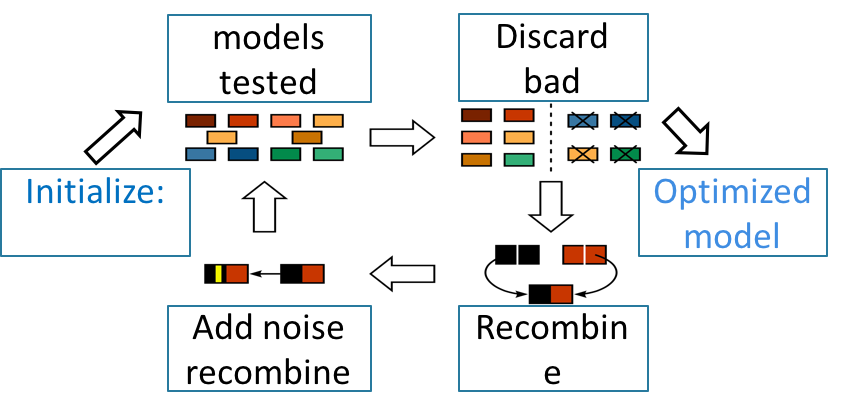
\includegraphics[width=0.7\linewidth]{figures/How_Genetic_Alg_Works.png}
  \caption{\textbf{Schematic of genetic algorithm flow.} Genetic algorithms find satisfactory solutions by incompletely sampling the solution space. Evolution of the algorithm is guided by the combined application of stochastic sampling and selective pressure. Stochastic contributions that guide GA sampling incentivise the exploration of regions beyond local minima. Stochasticity is applied in the combined actions of cross-over, and mutation. Model parameterizations are encoded as binary strings called genes. When genes breed, eligible pairs of genes are aligned and at random bit locations, the status of a bit is exchanged.  
}
  \label{fig:GeneticAlgOver}
\end{center}

\end{figure}
  
I use genetic algorithms in the work presented here, and while there are many variations on this approach, they all involve some combination of the following features:
% My GA picture belongs here
\subsubsection{Chromosomes}
In the context of genetic algorithms, a chromosome is the complete set of model parameters that are necessary to fully define the model being optimized, in this case a neuron model.
These parameter sets are collections of floating point numbers, for example -65.7 for a reversal potential in mV.
\subsubsection{Genes}
In the context of genetic algorithms, a gene is a single model parameter.  Consequently, the number of genes in a chromosome is equal to the number of parameters in the model.
There are at least two stochastic operations that over time provide a gentle "exploratory drive" for the algorithm, that cause genes to either double down on exploration of a local minimum, or possibly "jump" out of a local minimum to realize lower error.  These operations are applied, with some user-determined frequency, with each "generation" of the population of chromosomes, to determined the members of the subsequent generation.
\subsubsection{Simulated Genetic Recombination: Cross-over}
Cross-over is the exchange of genes between chromosomes.  In a population of many chromosomes, one can "mate" two of them, producing off-spring which represent a fraction of genes from parent 1 and the remainder from parent 2.  If each chromosome represents two opposing vertices of an n-dimensional hypercube (for n model parameters), then cross-over is capable of producing offspring representing any of the other vertices in that hypercube.
\subsubsection{Simulated Genetic Mutation}
A mutation reflects a (random) change to a single gene, i.e. a change to a single model parameter.  In some implementation this is achieved by flipping one bit in the binary representation of the floating-point value of the parameter, with the magnitude of the resulting change in the parameter value depending on which binary digit was flipped.  Often mutations are limited to a particular range for a given parameter.
\begin{figure}
%width=0.9
\begin{center}

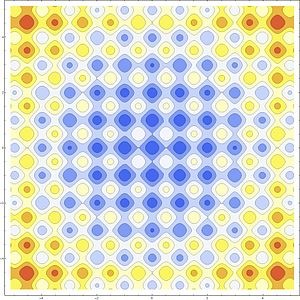
\includegraphics[scale=0.5]{figures/rastagrind}
\caption{Rastrigin's function is a function that is challenging to optimize, as it contains hundreds of local optima which would trap a gradient descent algorithm \cite{rastrigin1974systems}.}
\label{fig:rastrigin}

\end{center}

\end{figure}

\subsubsection{Elitism}
The number of chromosomes (model instantiations) in each generation is typically fixed, with some chromosomes in generation $n+1$ coming from crossover of chromosomes in generation $n$ and others from mutation.
The remainder are often chosen from the fittest, i.e. lowest error, members of generation $n$, a strategy known as elitism.
The degree of elitism essentially controls the amount of evolution that is allowed to occur in each generation.

\subsection{Multi-objective optimization} Multi-objective optimization problems are a subset of optimization problems.
In a multi-objective optimization, model fitness is evaluated using multiple "objective functions" of model fitness, each contributing either independently or in conjunction to the error surface.
Each function may ask a different question about the model; for example, one may ask how well the model reproduces the shapes of action potentials, and another function may ask how well the model reproduces the counts of action potentials.
The output of each such function is a scalar, with a lower values representing greater model/data agreement, i.e. lower error.
These functions are sometimes called constraints. 

\subsubsection{Weighted optimization} A simple strategy is to turn a multi-objective optimization problem into a single objective optimization problem, for example by summing the outputs of objective functions together. 
This is an extremely common strategy and has been the dominant approach in all neuroscience model optimization efforts to date [cite something here].
However, this approach comes with a significant price.
Optimization using a sum over multiple error measurements leads to a situation where a single constraint has an especially deep error surface, such that the gradient of the overall summed error surface is dominated by that single constraint.
In other words, minimizing overall error mostly corresponds to satisfying only one constraint.
The optimizer invests most of its search effort achieving a low error on one constraint, leaving the others unacceptably high.
This problem can in principle be ameliorated by re-scaling the objective functions to have similarly deep error surfaces, but in general the shapes of the error surfaces cannot be known in advance, so this sort of approach cannot generalize.\\

\subsubsection{Non-dominated Sort} A less appreciated but perhaps more important drawback to collapsing multiple objectives to a single one is that it imposes an opinion about the relative importance of each objective.
However, while there may underlying "true values" for measured biological variables, there is no underlying truth about which variables are more important than others.
In problems where not all measurements can be perfectly replicated by models (in part because the models are simplifications of biology), this problem becomes even more pressing.
The experimental data may also come from multiple data sources, leading to solutions for a single objective that reflect the diversity of the underlying system (e.g. physiological diversity of neurons of a given type), which is lost with the collapse to a single objective.

A multi-objective optimization paradigm that admits diverse sets of solutions to a list of constraints might better reflect biology, while also imposing less opinion about which measurements are most important.
The so-called "non-dominated sort" is one such paradigm.
It considers each objective function separately, and only considers one chromosome to be superior to another if it "dominates" that other, meaning that the objective function output is lower (i.e. smaller error) for each objective function.
If even a single objective function has a larger value for the latter chromosome, then it is not dominated.  Any chromosome that is not dominated by any other chromosome is considered "non-dominated" and is retained (i.e. for mutation, cross-over, or elitist selection) into the next generation.

The non-dominated set of chromosomes has a simple interpretation: each of its members would minimize a single, weighted objective function for some set of weights.
If no other chromosome has strictly equal-or-lower objective function evaluation for all constraints, then there exists a linear combination of weights which would give that chromosome the minimal evaluation (minimal error, maximal fitness) across the entire population.
Thus, retaining this population is equivalent to retaining all possible "opinions" about appropriate weights for the entire optimization process.

The NSGA2 algorithm \cite{deb2000fast} is a common implementation of this strategy, and is used throughout this work. Its performance can be compared to, for example, an exhaustive "grid search" across sets of model parameters, at least in low dimensions.  

\subsection{The Curse of Dimensionality}
Brute-force exploration of parameter space requires computation time that scales exponentially with the number of parameters.  In contrast, more efficient searches can be polynomial (e.g. linear or quadratic) in dimension number.  However, if constraints are weak, or conflicting, or the error surface is especially non-convex, many of these gains are lost, and exponential search times may return.  Thus, there is no guarantee in advance that reduced model optimization, with existing experimental data, is a problem that can be solved in reasonable time for sufficiently high-dimensional reduced models.

% First include a section about NeuronUnit more generally.  NeuronUnit really isn't/wasn't about optimization until your thesis.  
\section{Data Fitting and Optimization with NeuronUnit}
The ASU ICON laboratory previously developed a Python package called "SciUnit" for scoring scientific models according to their agreement with various experimentally-derived data (encoded as "validation tests") \cite{omar2014collaborative}.  The objective functions that I use here are implemented using this scoring process.
In particular, I used a SciUnit-based Python library called "NeuronUnit" which provides a number of such validation tests for neuron models, and I developed additional tests in the course of my research.

\subsection{Constraint Scoring}
The scoring mechanism within these tests determines the output of each objective function to be minimized.  There are many candidate scoring mechanisms, depending on what one means by "the model agrees with the data".  Each first computes some summary of model output, for example the resting membrane potential, called a "feature".
Here, the two most frequently used scoring mechanisms are: (1) compute the ratio between the model output feature and the experimental data feature mean, and (2) compute a Z-score reflecting the normalized distance between the model output feature and the distribution of experimental data features.
In both cases, the relevant experimental data distribution might be within trials, across trials, across recorded cells, or even across labs, producing many sources of hetereogeneity.
For example, resting membrane potential (measured in $(mV)$), may vary in some dataset according to a distribution with a mean and standard deviation of $(\mu,\sigma)=(-65mV,15mV)$.
The optimizer may sample a model (with some parameters) with a simulated resting potential of $-68mV$.  
NeuronUnit would then use these values to compute a Z-Score of $(-68 - (-65)/15 = 0.2$.
A model with a Z-Score of 0 would reflect perfect agreement with experimental data, and very low or very high values would represent poor agreement.
Our lab previously showed models can be scored on very large numbers of such tests, corresponding to experimental data for particular neuron types, and then used to build biophysically detailed neuron models for the mammalian olfactory bulb \cite{birgiolas2019towards}.

\subsection{Data Aggregation}
NeuronUnit thus converts a quantitative measure of model/data agreement into a useful error signal that can guide model optimization.
But a second function of NeuronUnit is to aggregate the relevant experimental data, in order to make  construction of the tests described above possible.
And a third function is to apply some signal processing and feature extraction steps to these data in order to produce something that can be scored.
These features were present at the beginning of this project, but I have extended them to cover more datasets and more features, as described in the Methods.

\section{Model Simulation and Exchange}
%%%%
% These ideas take up space, and they are theoritical 
% they don't yet reflect things that I actually did
% I will find a way to port the models to ML formats 
% after graduation. NeuroML didn't help me to optimize models
% A related effort the OSB was more helpful for cross-validation, and sourcing model parameters.
%%%
The NEURON \cite{carnevale2006neuron} simulator is a software suite that wraps powerful and fast ordinary differential equation solvers based in the C programming language inside a mixed compiled/interpreted environment targeted at research scientists. NEURON is somewhat analogous to older, analog circuit simulators;
however, rather than describing complex resistor-capacitor circuits, NEURON instead solves equations for the time varying membrane potential of multi-compartment models.

In contrast to reduced models, multi-compartmental models digitally encode the form of membrane tissue: cables of varying diameters and lengths that represent the morphology of neurons, and these cables support smaller scale representations of ion channels, and ion currents in the membranes.
These neuronal models can be coupled together into a network, where the electrical state of one neuron has an impact on the state of coupled neurons through synaptic currents.
Specifying the system of differential equations representing these neuronal morphologies, ion channels, and synaptic connections is complicated, but \emph{NEURON} makes multi-compartment neuron simulation efficient, convenient, and achievable.
Models expressed in \emph{NEURON} code are procedural in nature, and the code consists of low-level implementation details.
Procedural descriptions of models are difficult to extend and re-use, leading to a need for a declarative model description language.

NeuroML \cite{gleeson2010neuroml} is an extensible markup language (XML) tasked with describing these complex network models.
In principle, any simulator (not just NEURON) can execute a simulation based on a NeuroML file, so NeuroML models are readily executed across different types of simulators (ideally with identical results).
This facility makes NeuroML an excellent format for model sharing, and permits cross-examination of results if they vary across simulators, but also allows different modeling communities to retain the tools that they know best.
Because NeuroML is extensible and component based, it also incentivizes a "plug-in" environment for re-using existing model components in large-scale models for different contexts.
These existing components may include reduced models, for example embedded into larger neural circuits.
-
Open Source Brain \cite{gleeson2019open} is a collaborative, model development environment based on the NeuroML format, which contains collections of model-descriptions and model implementations, along with tools for simulation and visualization. These collections are well tested and understood, and the Open Source Brain platform was a practical tool for calibrating the models created for optimization in this work.

NEURON focuses on efficient simulation of multi-compartmental models, while NeuroML provides for model exchange. 
However, neither tool was designed with the optimization of reduced models in mind.
In optimization, the same model may be re-executed hundreds of thousands of times (with different parameter sets), so any computational overhead (for example, associated with reading/writing a file) is quite costly.  
There are other tools that may result in faster optimizations, but as I show here, even these are not optimally fast.
Consequently, it is best to think of tools like NEURON and NeuroML has useful for running and sharing optimized models, but not necessarily useful for the optimization process.  

\section{Analysis of Model and Experimental Variance}
It is common to observe large variations in measurements of a single electrophysiological entity from neurons of the same classification \cite{tripathy2014neuroelectro}.
For example, measured input resistance may be different when recorded from different cerebellar Purkinje cells.
Such differences may be due to intrinsic physical differences in cells (for example different surface area), due to differences in experimental methods across organisms or investigators, or simply due to the finite and limited number of samples available in the experimental literature.  
Aggregated data have been collected from mice, rats, marmosets, macaques, or even humans, where human data may have been collected under any number of disease states.

Understanding and modeling within-neuron-type variation should be considered an essential component of the scientific merit of computational modeling of a neuron-type.
However, the impact of this experimental variation on the production of neuron-type-specific models has not previously been explored.
Consequently, I will present here a large-scale analysis of the consequences of this variability--across many electrophysiological features--on the effort to produce canonical reduced models of several common neuron-types.
We would like to understand whether the space of existing or potential neuron models accurately represents the variability in the experimental data, and to help researchers map data collected from a number of experimental preparations onto a standardized rodent electrophysiological phenotype space.

\subsection{Relationship between Missing Data Imputation and Optimization}
Existing data sets are incomplete, consisting of a sparse sampling of cells in the rodent brain. By necessity, models are constrained using these incomplete data sets.
These missing data occur at multiple levels including exact neuron to neuron wiring patterns, un-sampled morphologies, unknown synapse activation times, and unknown axon and dendrite synapse locations.
More relevant to reduced models, even very basic information about spiking patterns in response to simple current injections may be unavailable.
However, since most fast numerical methods are incompatible with missing data, an additional component of model development--especially in the context of optimization--remains, which is the synthesis of plausible missing values.

\subsection{Closed Loop Development}
The speed of simulation is critical to successful optimization. However, even when using High Performance Computing (HPC) resources, errors may arise and require special handling or visualizations to diagnose.  These errors may even reveal that the model is mis-specified, but this may not be revealed until thousands of simulations have already run.
The ability to address and correct such mistakes requires rapid and verbose feedback during optimization, as well as simulations of sufficient speed to allow error "breakpoints" to be reached in a reasonable amount of time.

\subsection{Successful Optimization} 
Integrating the above ideas, I aimed to develop a framework for rapid, debuggable optimization of reduced neuron models subject to multiple constraints forged by experimental data, and to use this framework to optimize and share such models.
Here I will describe a number of methods and simulation experiments which demonstrate the successful implementation of many of these ideas, focusing on genetic algorithms that retain a diverse set of model parameterizations, potentially reflecting  within-type neuronal diversity.

The interactions between model constraints cannot always be known in advance, and in fact some constraints are mutually exclusive, either causing optimization to fail, or leading to a compromise. I also aimed to catalog such cases and use this knowledge to produce a more robust set of constraints, implemented via \emph{NeuronUnit} tests for future optimization work.

No model--including those that are published-- should be regarded as final.
Instead, I aimed to develop tools to improve these models by making them agree with experimental data, in the hopes that such models may be of general use to the neuroscience community in future work.
At best, replacing complex cell models with simplified models is a way to reduce the complexity of electrical brain activity to fundamental mechanisms \cite{teeter2018generalized}. At worst, simplified cell models may capture only a subset or a single aspect of important traits such as spike times \cite{hertag2012approximation}. %Many approaches to parameter fitting are limited to making models that reproduce spike times \cite{}

A simple way to fit a model to an experiment involves computing the difference between modelled waveforms and recorded waveforms. Computing the root mean square error between the two vectors, might seem like an appropriate approach, however, the $RMSE$  will be unduly more sensitive to spike timing and not as sensitive to agreement in spike shapes that occur at different times. It's very possible that a neuroscientist may care more about modelling the spike shape, than the spike time, and to address this missing need, we have appropriately decided to extract spike shape features from waveforms and to use these as our distance metrics.

When comparing two waveforms "proportion of variance explained" $(VE)$ is often used to overcome limitations in RMSE. \cite{schoppe2016measuring}. An alternative to this approach, is to select only a few electrical features from the recorded waveform that are deemed to be important, and to fit to those limited feature sets to experiments instead. A feature based approach to data fitting, is more likely to produce models that are not over-fitted, less fitted to noise, and models which generalize better. For example consider a neuron recording that contains $15$ spikes, and a model undergoing fitting to the data which has produced a waveform containing $16$ spikes. The VE of these two different waveforms might be quiet low, whereas the waveform shapes between model and experiment might agree on important features, such as spike width and height, and the voltage between spikes.


We chose to fit models to selected electrical features of the waveform, instead of simply fitting voltage traces, by 
% direct qoute -- "Creating simplified models is a way to reduce the complexity of the brain to its most fundamental mechanisms. In addition to the benefits of clarifying mechanisms for single-neuron behavior, single-neuron models can be used in larger network models that attempt to explain network computation. Thus, many models of a wide range of complexity have been developed to describe and recreate various aspects of neuronal behavior3. For an in-depth characterization of the diversity of neuron models, see the review4, and for their capacity to reproduce spike times see ref. 5.."


There are currently many optimization packages for optimizing multi-compartment conductance based models \cite{friedrich2014flexible} \cite{bluepyopt} \cite{neurotune},  these optimization packages are exclusively intended to work with the \emph{NEURON} simulator. There are at least two packages for optimizing reduced neuronal models, but one the these packages is used to fit models to spike times \cite{rossant2010automatic}, not spike shapes. This optimization framework uses specialized hardware and software GPU and CUDA, so this solution is not accessible to the average neuronal modeller.

%to fit models brian2 uses never-grad a python genetic algorithm frame-work that is principally related to DEAP
Additionally, the brian2 simulator supports some model fitting
\cite{brian2modelfitting},\cite{stimberg2019brian}. Although brian2 can fit spike shapes by comparing traces, the type of optimization performed is not multiobjective, as it computes the the $RMSE$ of whole waveforms, and uses it as a single objective error function. brian2 can also optimizes on spike times, but its not clear if it does this in a multiobjective context. Additionally, performance of brian2 was not reliable.

%or spike times plus spike shapes.

%To the best of my knowledge few or no python modules exist for the optimization of generic reduced neuronal models, that also optimize spike shape. 

Some core components of the optimization procedure detailed here do not deviate from those described elsewhere \citep{druckmann2008evaluating,bluepyopt}. Both of these optimization approaches use a multi-objective feature-based framework; however, there are several key differences. Critically, in this work we fit reduced models instead of conductance-based models, and this work seeks to formalize the quality of fits using Z-score, $\chi^{2}$ distributions, allowing us to compare the overall quality of data driven fits within and between model types. This allows us to answer questions such as: "Does one model type lead to better fits?" and "Are some \emph{in vivo} neuron measurements outside of the reduced model parameter scope?" Additionally, in this body of research we fit models using a novel range of electrical properties. One such property is the firing rate versus current (FI) slope, which is chosen to guide optimization because it produces models that are believed to be pre-tuned for use in networks. Models that fit the same FI-slope have the ability to fire at prescribed rates for a given amount of excitatory current. It is important that network neurons are calibrated in this respect, such that the behavior of the modelled network has  balanced firing rates and realistic interspike intervals.
\chapter{Methods}
In addition to the deployment of existing methods to achieve my research goals, this dissertation contains a number of innovations which are best described as methodological.  I include some of these innovations here, especially those of an extremely technical nature.  Some other methodological innovations, especially those of more interest to the computational neuroscience community, are reported later in the Results chapters.

\section{Approach to optimization using NeuronUnit}
Model optimization follows the following basic approach:
\begin{enumerate}
	\item Identify a model class whose parameters are to be optimized, e.g. the Izhikevich model.
	\item Identify a neuron whose experimental data will be used to guide optimization.
	\item Identify a suite of tests that can use that experimental data to guide the optimizer.
	\item Execute optimization of that model class against that suite of tests to return an optimized model.
\end{enumerate}
Within these steps are also a number of smaller decisions, including where the experimental data will be obtained and what kind of simulator will be used to run the model.
Using NeuronUnit, the steps above take the follow pseudo-code form:
\clearpage
%\begin{lstlisting}[language=python]
\begin{minted}{python}

# Import code from NeuronUnit
from sciunit import TestSuite
from neuronunit.models import MyModelClass
from neuronunit.tests import MyTestClass1, MyTestClass2, MyTestClass3
from neuronunit.data import get_data_from_database_x

# Get data about some neuron
neuron_type = "CA1 Pyramidal Cell"
neural_data = get_data_from_database_x(neuron_type)
test1 = MyTestClass1(neural_data[1]) # Test based on data feature 1
test2 = MyTestClass2(neural_data[2]) # Test based on data feature 2
test_suite = TestSuite([test1, test2])

# Optimize a model against this test suite
optimized_model = test_suite.optimize(MyModelClass)
\end{minted}
%\end{lstlisting}

Often model data is streamed from a remote machine for example NeuroML-DB. In that case local simulator capabilities are not required in order to make streaming models eligible for Neuronunit tests. The code idiom for working with streaming models is as follows:

\begin{minted}{python}
import requests
from neuronunit.models import static_model as sm
model_scores = []
for data in NeuroMLDB_requests:
    remote_model = requests.get(data)
    vm = remote_model['vm']
    SM = sm.StaticModel(vm)
    score = test_suite.judge(SM)
    model_scores.append(score)
\end{minted}


%\section{Approach to Optimization using NeuronUnit}
Model optimization follows the following basic approach:
\begin{enumerate}
	\item Identify a model class whose parameters are to be optimized, e.g. the Izhikevich model.
	\item Identify a neuron whose experimental data will be used to guide optimization.
	\item Identify a suite of tests that can use that experimental data to guide the optimizer.
	\item Execute optimization of that model class against that suite of tests to return an optimized model.
\end{enumerate}
Within these steps are also a number of smaller decisions, including where the experimental data will be obtained and what kind of simulator will be used to run the model.

Using NeuronUnit, the steps above take the follow pseudo-code form:

\begin{lstlisting}[language=python]
# Import code from NeuronUnit
from sciunit import TestSuite
from neuronunit.models import MyModelClass
from neuronunit.tests import MyTestClass1, MyTestClass2, MyTestClass3
from neuronunit.data import get_data_from_database_x

# Get data about my neuron
neuron_type = "Layer 5 pyramidal Neuron"
neural_data = get_data_from_database_x(neuron_type)
test1 = MyTestClass1(observation=neural_data)
test_suite = TestSuite([test1, test2, test3])
results = test_suite.optimize(model)
\end{lstlisting}

There are two different paradigms for evaluating models in NeuronUnit. Under the first paradigm the model is supported by NeuronUnit, and dynamic simulations of the model are present on the host computer and can be efficiently re-run.

Under the second paradigm the NeuronUnit version of the model only consists of model inputs and outputs that are streamed as needed from a different environment. This may be the case due to the complexity of the model, where re-implementing the model would not improve clarity. Or the full model may exist on a remote machine with outputs accessed via an API. 
%Another way of saying this is that if a "model" is simply a digitized set of waveforms, converting it to a model is as simple as labeling things such that NeuronUnit and the scientist are both consistent about what is a model and what isn't. 
The optimization procedures I describe in this work involve both paradigms, where optimizing within the second paradigm required dedicated code that is not supported within the previously described frameworks.

\section{Model Class Implementations}
Because optimization may involve an extremely large number of independent simulations of the same class of model, each varying only in model parameter values, it is critical that both the overhead for model instantiation and the duration of simulation be as low as possible. We built faster Python implementations of two neuronal models -- the Izhikevich model and the adaptive exponential integrate and fire model. My implementations of the Izhikevich model was based on an existing MATLAB forward Euler implementation, while my implementation of the adaptive exponential integrate and fire model came from vectorized Python code, which was relatively slow.

I was able to use a tool to make both of these models perform faster than the standard versions for the brian2 and NEURON simulators. This tool, \cite{numba}, enables Just In Time compilation (JIT).
 %Without over stating things, 
 When regarding this thesis effort and its contribution to knowledge, some of the value to the neuroscience modelling community comes from the implementation of these two fast Python neural model simulations. Because these simulations are written in Python, the code that implementations them is easy to understand share and execute, because the models are fast to dispatch they are useful in both network and optimization contexts where performance is critical. 
 
%A component of this work the Izhikevich model, I plan to push to the Open Source Brain %\href{https://github.com/russelljjarvis/IzhikevichModel.git}

\subsubsection{Why Existing Approaches Were Not workable}
In this research effort significant time was spent shoe-horning pre-existing tools into an optimization frame work, with limited success. These tools included:  PyNN, brain2, \emph{NEURON}, jNeuroML-2. However, several unexpected road blocks were encountered on the way.
 
When applying reduced models to optimization, there was a cluster of known errors and limitations in pre-existing community standard reduced model simulators. 

To make optimization of models tractable it was important to do ongoing feasibility testing. For example its important to evaluate the the utility of established model implementations, as using these models to optimize may not in fact be feasible.\\ 
Despite an a large number of choices of FOSS reduced model implementations, many off the shelf implementations were not useful, or significant intervention was required to make some established implementations workable inside an optimization framework. \\
 
Some revisions to the Izhikevich model include equation tweaks, in order to let cells better reproduce in-vivo firing dynamics, such as bursting, and re-bound spiking \url{https://github.com/OpenSourceBrain/IzhikevichModel/blob/master/MATLAB/izhi2007.m}. However, when multiple equations, however closely related, are incorporated under the same umbrella, this fractures the implementation of the model into sub-models. The \emph{NEURON} implementation of the Izhikevich model is fractured. There are different implementations for different regimes. This meant that switching between model regimes during optimization would be a non-trivial exercise because the is already splintered between two languages (NEURON, NMODL, python), the source code would be highly complicated such that it would not be readable, and it would loose generality, overly customized towards one target model. The NEURON code, needed NMODL files to be compiled for each different regime, and promised performance of the C based NEURON library was not actualized. The only benefit to using this model, was that its parameter ranges are well tested and understood within OSB and NeuroML-2 community.

Because the PyNN implementations of the Izhikevich models are "wrapped" versions of essentially NEURON models, PyNN models still retained the disadvantages of the NEURON models (surprisingly poor speed on the Izhikevich model) while introducing other problems. PyNN is designed to preference the description and implementation network simulations. A data-type called a "lazy-array" is the smallest elemental container for neuron models in PyNN, but it is meant to store populations of neurons as opposed to single neurons, as such the lazy-array often slows down and gets in the way of the single neuron simulations, which model fitting depends on.
%(lazy array evaluation). 

 Sub models $[1-3]$ are really different parameterizations of the same equation, sub-models $[4-7]$ are actually different equations, meaning that there is a total of $4$ Izhikevich sub-models. To permit optimizer access to the broadest range of Izhikevich dynamics, a new meta-parameter $cell_type$, was created. This number ranging $[3-7]$ (unique model equations included only), allows the optimizer to change which Izhikevich sub-model it samples from. Later in on in results, we see that in fact even when fitting to static electrical properties, optimizer access to the broader set of firing regimes improved the quality of fits.


%The described limitations of the 
%https://github.com/NeuralEnsemble/PyNN/issues/370$%}, journal={GitHub}, author={Davison A}
%}


%@misc{neuralensembleadexp, title={pyNN.neuron %implementation of AdExp is unstable, gives poor results  Issue $#266 · NeuralEnsemble/PyNN$}, url={$https://github.com/NeuralEnsemble/PyNN/issues/266$}, journal={GitHub}, author={Davison A.}
%}
\url{https://github.com/NeuralEnsemble/PyNN/issues/370} 
%\cite{neuralensemble_adexp}
\url{https://github.com/NeuralEnsemble/PyNN/issues/266} 
%\cite{neuralensemble_adexp2}
 
A constant error warning plagued brian2 investmentallations was.
\begin{verbatim}
Brian2 causes error:
 ERROR      Brian 2 encountered an unexpected error. If you think this is bug in Brian 2, please report this issue either to the mailing list at <http://groups.google.com/group/brian-development/>, or to the issue tracker at <https://github.com/brian-team/brian2/issues>. Please include this file with debug information in your report: /tmp/brian_debug_t0acbm4l.log  Additionally, you can also include a copy of the script that was run, available at: /tmp/brian_script_juzhsbph.py Thanks! [brian2]
Traceback (most recent call last):
\end{verbatim}
In two classes of model a feasible choice of implementation did not exist and it was easier to re-implement those models. The two models I re-implemented were
the Adaptive Exponential Integrate and fire Model, and also the IZHI
model.  In the work below, I profile existing model implementations, and
justify the reasons for re-implementing.\\
\\
This is in contrast to the brian2/neuraldynamics AdExp model, which took
between 2 or 3 times longer to find a rheobase current injection value. However the slowness is not caused by the simulation backend (brian2 which is relatively fast and efficient). The slow down is caused by the way the model is defined. Specifically the
model is defined in a middle code layer neurodynamics \cite{gerstner2014neuronal}.\\
\\
It is very likely, that the model implementation is correct, since Gerstner is an author of one of the original adaptive exponential publications, and the neural dynamics book that the brian2 code is strongly affiliated with. Since Integrate and Fire models don't formally include spikes when an implementation does include spikes, it is an optional add on.\\
\\
The AdExp neurodynamics models default implementation causes spikes with peaks below $0mV$, since the IZHI model like all integrate and fire models do not explicitly include spikes\\
\\
This is not technically wrong, but it violates
assumptions in the \emph{NeuronUnit} feature extraction protocol. The default spiking behavior, looks odd, and it is simply this poor model definition that is causing a slower optimizer performance. The optimizer takes an unusual waveform shape, and searches for longer in distant
parameter regions to find a good fit.\\
\\
Over the course of evaluating the brian neural dynamics model \cite{gerstner2014neuronal}. I experienced some phenomena that only occurred in the context of genetic algorithm optimization. The reason why optimization provides a different evaluation context is because, in optimization simulation objects are required to be created and destroyed rapidly and on mass. Brian2 is designed to be an efficient network simulator, the case of being designed for network simulation, may assume you will want to create a lot of neural models that persist efficiently together in memory (this was also a problem with PyNN models). Therefore you might see below, that while only one brian model exists in memory, performance is okay, but when creating and destroying models rapidly and on mass a slow down occurs.\\
\\
Below I have implemented a Python integrator for the adaptive exponential integrate and fire model. This solver led to faster evaluations of current injection experiments. The integrator I developed has a $0mV$ spike when evaluated at default parameter values.\\

Brian2 and SciUnit sometimes collided in name space and logging.
%\href{https://github.com/scidash/sciunit/pull/124/files/83907ba68740642178ebb91084f6e382e06a43c4#diff-d68791d2ed5dfaa96a900be6180bd950}

\section{Profiling the JIT Enabled AdExp Model}
Mean time taken on single model evaluation:$ 0.0012554397583007812s $
Mean time taken to compute Rheobase:
$0.183s $
This was slightly faster than Izhikevich implementation which was for total rheobase solution $ 0.462s $ and $  0.002 s$ per run. Solving for Rheobase takes a average of 15 model evaluations.
%\begin{figure}    
%\begin{center}
%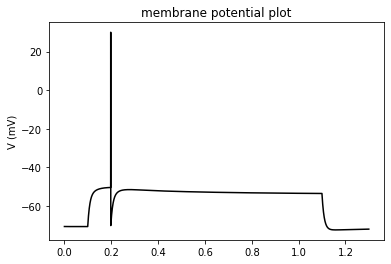
\includegraphics[width=0.25\linewidth]{figures/backend_check_files/backend_check_6_2.png}
%\caption{}

%\end{center}
%\end{figure}

%\begin{verbatim}
%    251 ms +- 5.02 ms per loop (mean +- std. dev. of 2 runs, 1 loop each)
%    240 ms +- 11.1 ms per loop (mean +- std. dev. of 2 runs, 1 loop each)
%    223 ms +- 12.5 ms per loop (mean +- std. dev. of 2 runs, 1 loop each)
%\end{verbatim}

\begin{verbatim}
    922 ms +- 12.7 ms per loop (mean +- std. dev. of 7 runs, 1 loop each)
\end{verbatim}

\subsection{Comparison of Parallel and Serial Speeds and Accuracy}

Below is the Brian2/NeuralDynamics AdExp model. In-order to make the spike height greater than $0mV$ it was easier to use computer code to schedule waveform modifications that occur straight after the the brian2 simulation, these scheduled waveform modifications can be considered part of a peripheral shell of simulation code. In postprocessing
the waveform data type is a Neo Wave form object that is artificially the algorithm of determining rheobase and displaying results. The time of this model is determined on multiple factors, as discussed elsewhere, execution time is not uniform across model parameterizations. Models with multispiking behavior will take longer to solve.

Simulation times for this model vary, dramatically possibly because of
lazy evaluation, the simulation times may vary according to what else
you are running on your computer. Not all models experience a speed up when executed in parallel, however
this model was faster in the parallel Rheobase determination algorithm. Some common times are: $3.92,6.75,4.48,5.17$. Mean time was:

\subsection{Comparison of Time to Find Rheobase}

Custom implementation JIT enabled implementation: $4.0s$. 
Brian2 taken to find Rheobase: $4.40s$ (serial), $3.976s$ (parallel).

The evaluation times between Brian2 and the custom written
integrator are similar. Both have average rheobase solution times of approximately 4 seconds, however the spike shape derived from the custom written integrator look more realistic under default paramaterizations. The biological plausibility of default model paramaterization has consequences for model optimization speed, because when  models undergo mutation and cross-over the mean of random models regressors towards the default model initialization, and if the default model is a bad fit to data, the average model sampled by the genetic algorithm will also be bad to data.\\

\begin{figure}
\centering
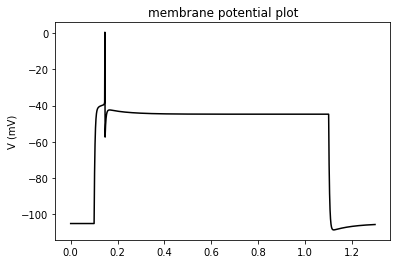
\includegraphics[scale=0.45]{figures/backend_check_files/backend_check_12_10}
\caption{Model Parameterization of the brian2 Simulator with the customization: interpolated spike height, forced to be above $0mV$}
\label{fig:sub1}
\end{figure}

\begin{figure}
\centering
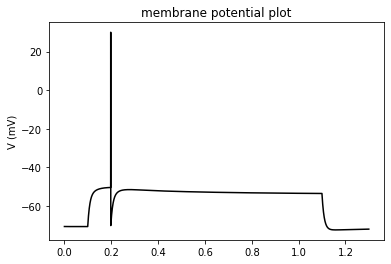
\includegraphics[scale=0.45]{figures/backend_check_files/backend_check_4_2}
\caption{Default model parameterization of the custom written integrator}
\label{fig:sub2}
\caption{Comparison between two Adxaptive Exponential Implementations}
\label{fig:test}
\end{figure}




    
$272 ms +- 66.5 $/mu$s per loop (mean +- std. dev. of 2 runs, 1$ loop each)

The next model to be evaluated is the NEURON Izhikevich model. The NEURON Izhikevich model has various draw backs. 1. It depends on an external file which must be recompiled each time this project is recreated. 2. The build environment of NEURON is non-trivial, and only a super dedicated NEURON modeller would install it on their system. Any performance advantage of using NEURON investment does not exceed the installation cost of installing the program. 3. The model implementation code is less generalizable than than the published Izhikevich model itself. Where the standard NEURON-NeuroML code only covers the Regular-Spiking model * This is likely due to a name space conflict between Capacitance. Neuron has a `capacitive' mechanism inside modelled Neurons, this particular model has section capacitance as well as an introduced capacitive term inside a C-compiled mechanism. Both contribute to a the membrane
potential calculation. * The NEURON Izhi model took $78$ seconds to find the rheobase current injection value $ 51.79367065 * pA $.

    
%\begin{center}
 %   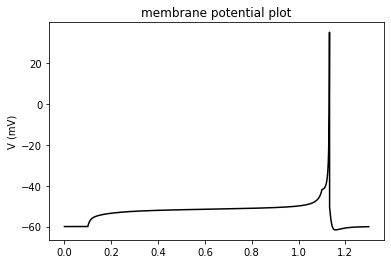
\includegraphics[width=0.7\textwidth,]{chapters/figures/backend_check_files/backend_check_14_2.png}
%    \caption{where is picture}
%\end{center}


%\begin{figure}
%    \centering
%    \includegraphics{chapters/normal_distribution}
%    \caption{This is your image%}
%    \label{fig:my_label}
%\end{figure}
%A tool numba JIT

% https://www.overleaf.com/learn/how-to/Images_not_showing_up 

        
The enabled forward Euler python Izhikevich model was very fast. The forward euler
implementation utilized Numba JIT \cite{lam2015numba}. Rheobase is found in under a second,
and in many cases close 0.5 seconds. This represents a very dramatic
speed up. Unlike the NEURON NeuroML implementation of the izhikitich equation,
this implementation is just as generalizable as the original MATLAB
implementation of the Izhikevich model, because it was possible to unify the fractured implementations in the one python simulator backend.

\subsection{NEURON+Python single compartment Conductance Model.}

Conductance based models took approximately the same amount of time to evaluate the Rheobase search algorithm as the python implementation.

The author also engineered GLIF model support for $NeuronUnit$ tests. In practice these models where hard to configure without expert knowledge, GLIF models contain the most parameters of all models, and many of these parameters are multi dimensional. GLIF models do not by necessity spike, interpolated spike times, are added in however, it does not make sense to evaluate GLIF models on spike shape features.

It is worth noting that the layer 5 neocortical pyramidal neuron was very slow to dispatch relative to the reduced models developed in this thesis work. Where as a typical reduced model described here evaluated in the order of $2.5 ms$, this model on average took $5.74$s, for a single run and $34.8$s to solve for the models Rheobase, current. To be fair, the model was run without activating NEURONs variable time step cvode. However, even with variable time step applied to the differential equation solver the magnitude of the disparity is still still several $seconds:$ several $ ms$. 

% time taken to compute rheobase $ 12.6s $


%\begin{verbatim}
%  time taken on
%  block 0.6859951019287109 \textbackslash{}n3.3 ms +- 9.79 %$\mu$s per loop (mean +- std. dev. of 2
%  runs, 100 loops each)\textbackslash{}n3.32 ms +- 30.9 us per loop (mean +- std. dev. of 2 runs,
%  100 loops each)\textbackslash{}n3.19 ms +- 10.9 us per loop (mean +- std. dev. of 2 runs, 100
%\end{verbatim}
        


%This problem in the default parameterization of the python model was later located in the scale or units of capacitance, if default capacitance parameterization is multiplied by 100.0 the problem goes away.


%\begin{center}
%\includegraphics{figures/backend_check_files/backen%d_check_22_2}
%\end{center}

%$ 1.40762329 * pA $


% \subsection{NEURON versions of single compartment Conducance
% model.}

% Took $8.57$ seconds to find Rheobase.

%Hodgkin Huxley Conductance based channels models took approximately the same amount of time to evaluate the Rheobase search algorithm as the python implementation.

%The NEURON implementation was slightly faster, and the default parameterization of the model lacked `ringing'', or below threshold oscillations that the Python ODE version had under default conditions.

%This problem in the default parameterization of the python model was later located in the scale or units of capacitance, if default capacitance parameterization is multiplied by 100.0 the problem goes away.


%which makes debugging their behavior very difficult. %None the less GLIF models where among the fastest to evaluate, and the author had success in making fitting these models to Allen Rheobase data.

    %\graphicspath{ {../figures/} }
%    \begin{center}
%    \begin{figure}
%    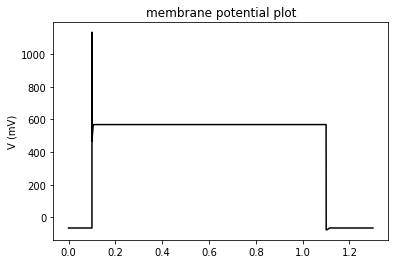
\includegraphics{figures/backend_check_files/backend_check_26_2}
    %kend_check_files/backend_check_26_2.png}
%    \end{figure}
    
%    \end{center}
%\begin{verbatim}
% 112.5 pA
%'value': array(1.40645904) * pA
%\end{verbatim}

% parameters of an adaptive exponential model
%\begin{verbatim}
%\{'El\_reference': -0.07016548013687134, %'C': 3.990452661875942e-10%,
%'init\_threshold': 0.02964956889477108, %'th\_inf': 0.02964956889477108,
%'spike\_cut\_length': 109.5, %'init\_voltage': -35.0, 'R\_input': %910258965.9792937\}
%\end{verbatim}
%$ Rheobase = 112.5pA $
%time taken to execute GLIF model when deliberately undersampling to save time.
%$ 0.23476457595825195 $

    


%$ 112.5 pA $
%$0.0 mV$ $-0.065 mV$

%    \begin{verbatim}
%    \{'value': array(183.33333333) * pA\}
%    \end{verbatim}

%\begin{verbatim}
%array(112.5) * pA
%\end{verbatim}


%\begin{verbatim}
%    0.017240506310425608 mV -0.08583939747094235 mV
%    0.017240506310425608 mV% -0.08583939747094235 mV
%\end{verbatim}

    %\begin{center}
    %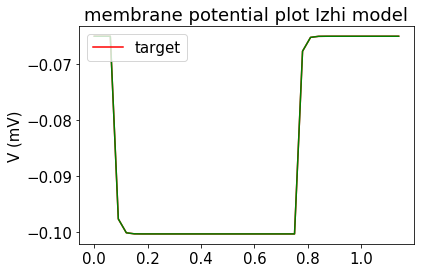
\includegraphics{figures/backend_check%_files/backend_check_32_2.png}
    %\end{center}

%\input{chapters/methods/rheobase}

\section{Pre-Existing Model Class Implementations}
First I accessed an implementation of the Izhikevich model that was translated from jNEUROML into a NEURON simulator implementation.
However, this implementation fragmented the family of Izhikevich models into chattering and non-chattering subtypes.
The model implementation also seemed to have an internal conflict between two capacitive terms and could not reproduce all of the original publication figures.
Although the NEURON simulator is designed to be fast, there is a cost associated with reloading the NEURON environment many times in fast succession, and implementation odel execution times were not brief enough to be useful for optimization.

\section{Other Model Class Implementations}
For various reasons described in detail below, existing implementations of some models were not adequate for this research.
These reasons included speed, generality, and consistency.

\subsection{Model Execution: The Need for Speed}
Because optimization may involve an extremely large number of independent simulations of the same class of model, each varying only in model parameter values, it is critical that both time costs--both the overhead for model instantiation and the duration of simulation itself--be as low as possible.
Existing modeling tools contain overhead associated with model initialization and shuttling results in memory.
These costs are trivial for single simulations, but begin to add up in optimization runs of thousands or even millions of simulations.  
Even the marginal cost of simulation--expressed as seconds on a wall clock per seconds of model output simulated--is often slower than expected using existing tools, due to some of these tools being written to accommodate more complex, biophysical models, rather than engineered for raw speed.
During optimization, many parameter sets are explored, and the speed of  simulation can be determined by the parameter values.
For example, those parameter sets which produce many spikes in a given simulation run more slowly, because $\frac{dV_{M}}{dt}$ changes rapidly throughout the simulation, necessitating reductions in simulation step size to avoid numerical instability.

\subsection{Model Design: Lack of Generality}
Significant time was spent in the early years of this project shoe-horning pre-existing tools into the desired optimization framework, with limited success.
These tools included, among others, model designers and neural simulators such as PyNN, Brian2, NEURON, and jNeuroML.
However, several unexpected road blocks were encountered on the way.

\subsubsection{NEURON}
The NEURON simulator is a very mature and respected neuron and neural network modelling framework \citep{carnevale2006neuron}. This simulator specializes in multi-compartment conductance based models of neurons and neuronal networks, but the simulator has also been made to accommodate many reduced model implementations. The NEURON implementation of the Izhikevich model is fractured in that there are different NEURON NMODL implementations of the equations for different parameter regimes.

When running only a single model simulation this is not much of a problem. However, switching between Izhikevich model regimes during optimization (as would occur when a parameter value crossed a regime boundary) is a non-trivial exercise.
Even if successful, any multi-language source code successfully implementing this would be complicated, unreadable, and lack generality.
Specifically, NEURON requires NMODL files to be compiled for each different regime, and it may be difficult to know in advance which regimes the optimizer is likely to sample from.
Additionally, the promise of fast performance due to the C-based NEURON library is not actualized with this model.
Because NEURON is well-understood within the OSB and NeuroML community, I used it only to produce reference simulations to verify that the output of my model implementations were in fact accurate according to community standards.

\subsubsection{PyNN}
PyNN provides the convenience of working in Python, and with a convenient procedural interface for model design and execution \citep{davison2009pynn}.
However, its implementations of most reduced models (e.g. Izhikevich) are simply ``wrapped" versions of NEURON models; consequently PyNN has the same disadvantages as NEURON.
PyNN is also designed with network simulations in mind, which means its designers have chosen performance trade-offs that favor network simulations over single neuron simulations.
For example, a data-type called the ``lazy-array" is the most elemental container for neuron models in PyNN, but it is meant to store populations of neurons as opposed to single neurons;
as such the lazy-array adds overhead to accessing single model results.

% in slow single neuron simulations.

Additionally, the NEURON implementations that underlie the PyNN-provided AdEx and Izhikevich model classes suffer from some fidelity issues under certain regimes and parameter sets, compromising optimization quality (see \cite{neuralensembleadexp2, neuralensembleadexp} for details).

\subsubsection{Brian2}
Brian2 \citep{stimberg2019brian} is, in principle, an excellent simulator for working with reduced neuron models, as it allows for differential equations to be expressed in an intuitive form, while also keeping track of dimensions and units.
However, it may not be mature enough for complex applications, as it produced errors in optimization contexts that did not occur during routine simulation of single-parameter sets.

Even when these errors did not occur, (e.g. using the Brian2 AdExp model), certain optimization steps (such as identifying the rheobase current for a given set of model parameters) took 2-3 times more simulation time then a reference approach (described in the next section).
This slowness was not caused by the simulation mechanics themselves (Brian2 is relatively fast and efficient, as described in \cite{stimberg2019brian}.)
Instead, these delays are caused by the way the model is internally defined, specifically using a
so-called ``neurodynamics" layer \citep{gerstner2014neuronal}.

While it is very likely that this implementation is useful and correct in many contexts (Gerstner is an author of one of the original AdEx model publications \citep{brette2005adaptive}, and the Brian2 implementation is derived directly from his work), it is problematic for the feature extraction step required in optimization.
Specifically, these implementations do not formally contain any notion of ``overshooting" spikes, since when the spike threshold is reached, the membrane potential is simply set to some reset value; the presence and timing of a spike is recorded only when a separate process is explicitly set to watch for such an event.
This is not technically wrong, but it violates a key assumption in the \emph{NeuronUnit} feature extraction protocol (the existence of an action potential waveform to extract), and the extra layer for detection of spiking adds computational overhead.
Imputing a spike-like waveform near threshold can help solve the problem, but then optimization results and performance becomes contingent on the design of this waveform imputation, and not on the model itself.

Lastly, over the course of evaluating the Brian neural dynamics model \citep{gerstner2014neuronal}, I encountered some problems specific to genetic algorithm optimization.
This context is not identical to simply running a series of simulations in series, because optimization operates in parallel, must fit into computer memory, and thus requires that simulation objects be created, simulated, and then destroyed rapidly and en masse.
Since Brian2 was designed for stability, is was not designed to make model disposal computationally efficient (the problem of clearing objects from memory efficiently is, from a computer science perspective, trickier than it might initially sound).
Therefore, performance of Brian2 suffered when I re-purposed its code to work in an optimization context.
Brian2 does support its own internal scheme for model fitting \citep{brian2modelfitting}, however this scheme was only published late in this thesis work, and it is unknown what technical tricks they employed to enforce model garbage collection. 
Additionally this scheme is highly divergent from the multi-objective DEAP framework described in Section \ref{sec:tech-details}, so it is not readily interoperable with the model fitting workflow described here.

\subsubsection{My Approach}
\label{sec:new-models}
In summary, despite several choices for existing, free, open-source software (FOSS) reduced model
implementations, these implementations were not useful, or significant intervention would have been required to apply them within an optimization framework.
To overcome this and accelerate optimization, I built faster ``direct" implementations of two neuronal models (the Izhikevich model and the AdEx model).
One of the these was inspired from the existing MATLAB forward Euler implementation of the Izhikevich model, while the other was adapted from an existing Python implementation of the AdEx model using vectorized code.
While neither of these was especially fast, they provided the basic recipe upon which a faster Python implementation could be built.
Do note that the purpose of these new implementations was not model exploration, analysis, or sharing; existing tools are adequate for these purposes.
The purpose of the new implementations was simply to make large optimization runs computationally tractable.

Although typically much faster than R, Python does not have a reputation for speed; implementation details have a large impact on performance.
Therefore, I used a tool called Numba \citep{lam2015numba} that enables Just-In-Time compilation (JIT) of Python code, making it comparable in speed to compiled C code.
This tool cannot be applied to any arbitrary Python code, so functions to which it is applied must be designed with only a fairly plain subset of the usual syntax and library of Python.
In other words, it cannot be used to simply speed up any pre-existing Python code.
%all code is hand-coded, even cutting and pasting is done by hand suggested synonym crafted.
I crafted the two model types above to be JIT-compliant, with the result that both became significantly faster than analogous models using NEURON or Brian2 simulators.
Importantly, simulation outputs retained a binary near-match in all cases, confirming that nothing was lost in the course of gaining this performance improvement.
I used these new implementations extensively throughout the project, and they are available to others at \cite{jithub}. 
The code that implements them is fairly easy to understand, share, and execute, and I hope they may be useful to others who have similar performance needs, either for optimization contexts or in large network models on generic commodity computer hardware where small performance gains are worth chasing. 

Some models were executed in their native implementations using the NEURON simulator with an adaptive time step.
After each model run, the variable time step vectors were resampled into fixed time step vectors using interpolation.
I accelerated this inherently slow process by applying the JIT framework to prior code contributed by a colleague \citep{birgiolas2019towards}.

Below, I profile my implementations and compare them to the existing FOSS implementations.
My implementations led to faster per-simulation evaluations of simulations involving somatic current injection. 
Furthermore, my implementation exhibited over-shooting spikes (spikes crossing 0 mV, as occurs in real neurons), making them more compatible with NeuronUnit feature extraction.

\subsection{Profiling the Models}
Obtaining the rheobase of a model for a single parameter set requires simulating it many times at different values of somatic current injection until the minimum action-potential inducing current is obtained (to within some tolerance; here I used 0.1 pA, near the standard deviation of thermal noise).
This takes 10-15 simulations, on average.
\begin{verbatim}
My AdExp implementation:
Single model simulation: 0.00126 s
Rheobase computation: 0.183 s

My Izhikevich implementation:
Single model simulation: 0.002 s
Rheobase computation: 0.462 s
\end{verbatim}

\subsubsection{Comparison of Speed and Accuracy Versus Brian2}
In-order to implement NeuronUnit-compatible Brian2 AdEx model simulations, I imputed spike waveforms (at recorded spike locations) immediately following each simulation.
The simulation time of this model is determined by multiple factors, as discussed elsewhere. Execution time is also not uniform across model parameterizations; in particular, parameter sets exhibiting more spikes take longer to solve numerically.
I compared this with the same parameter sets in my implementation, with the results shown below:

A large fraction of the time spent simulating models under a single set of parameters is spent obtaining the rheobase current, upon which several subsequent tests and extracted features depend.

The JIT implementation of the AdExp model was approximately 1000$\times$ faster than the Brian2 model.
Another benefit of the JIT implementation was that it did not require imputation of action potential waveforms (as was required for the Brian2 implementation); without additional work, the JIT implementation produced much more realistic-looking action potential waveforms under most model parameterizations.
To the extent that action potential shape is an optimization target, this is a decisive advantage for the JIT implementation.

\begin{figure}[!htb]
\begin{center}
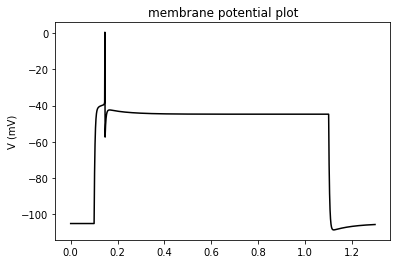
\includegraphics[scale=0.7]{figures/backend_check_files/backend_check_12_10.png}
\caption[Brian2 simulation of the AdEx Model]{\textbf{Brian2 Simulation of the AdEx Model.} Simulated membrane potential trace from the AdEx model at rheobase using the Brian2 simulator. The action potential waveform has been interpolated at the time when the simulator reported a spike.
The horizontal axis shows time in seconds.}
\label{fig:AdEx-Brian2-sim}
\end{center}
\end{figure}

\begin{figure}[!htb]
\begin{center}
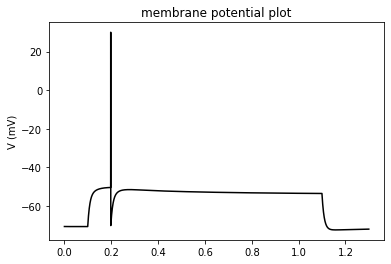
\includegraphics[scale=0.7]{figures/backend_check_files/backend_check_4_2.png}
\caption[JIT Simulation of the AdEx Model]{\textbf{JIT Simulation of the AdEx Model.} Simulated membrane potential trace from the AdEx model at rheobase using my JIT implementation. In contrast to Fig. \ref{fig:AdEx-Brian2-sim}, the dynamics of the action potential arise naturally from the integrated equations and do not require interpolation.}
\label{fig:AdEx-JIT-sim}
\end{center}
\end{figure}

\subsubsection{Comparison of Speed and Accuracy vs NEURON}
I also compared the performance of my implementation of the Izhikevich model to the one generated by NEURON from the OpenSourceBrain Izhikevich model NeuroML2 files.
This NEURON implementation has several drawbacks, including: 1) It depends on an external file which must be recompiled each time this project is recreated; 2) The build environment of NEURON is non-trivial; 3) The model implementation code is less generalizable than than the published Izhikevich model itself.
For example, the standard NEURON-NeuroML2 code only covers the Regular-Spiking flavors of this model, and does not support the full range of model parameterizations; 4) Name space conflicts between built-in NEURON parameters and Izhikevich model parameters.  

%\begin{center}
 %   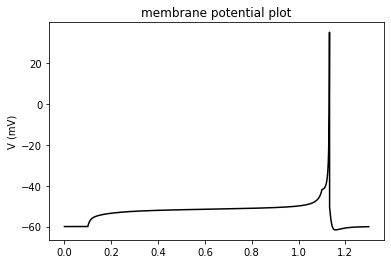
\includegraphics[width=0.7\textwidth,]{chapters/figures/backend_check_files/backend_check_14_2.png}
%    \caption{where is picture}
%\end{center}


%\begin{figure}
%    \centering
%    \includegraphics{chapters/normal_distribution}
%    \caption{This is your image%}
%    \label{fig:my_label}
%\end{figure}
%A tool numba JIT

% https://www.overleaf.com/learn/how-to/Images_not_showing_up 
        
The NEURON implementation of the Izhikevich model took $78$ seconds to identify the rheobase current.
In contrast, my implementation identified the rheobase in only $\tilde 0.5 s$.
This represents a very dramatic speed up, which can largely be attributed to overhead associated with initializing successive simulations.
Furthermore, my implementation generalizes to all possible parameter values for the Izhikevich model parameters, thus allowing for all of the many diverse spiking behaviors exhibited in the original publication by \cite{izhikevich2003simple}.

%\begin{verbatim}
%  time taken on
%  block 0.6859951019287109 \textbackslash{}n3.3 ms +- 9.79 %$\mu$s per loop (mean +- std. dev. of 2
%  runs, 100 loops each)\textbackslash{}n3.32 ms +- 30.9 us per loop (mean +- std. dev. of 2 runs,
%  100 loops each)\textbackslash{}n3.19 ms +- 10.9 us per loop (mean +- std. dev. of 2 runs, 100
%\end{verbatim}
        
%\subsubsection{Comparison of speed and accuracy vs NEURON for %conductance-based models}
%Could the relatively poor performance of existing implementations 5above be due the use of reduced models?
%I ran similar profiling exercises for a single-compartment %conductance-based model (implementing the Hodgkin-Huxley equations %\cite{rall1962electrophysiology}) to see whether the disparities %above persisted.
%I compared an existing Python implementation for simulation of %this model against the NEURON implementation.
%Conductance-based models took approximately the same amount of
%time ($12.6 s$ XXXX put in exact numbers) to determine the %rheobase as the existing Python
%implementation, suggesting that . XXXX What is this comparison?  %Conductance-based vs Python?

%\begin{center}
%\includegraphics{figures/backend_check_files/backen%d_check_22_2}
%\end{center}

%$ 1.40762329 * pA $
%XXXX Redundant? Hodgkin Huxley Conductance based channels models %took approximately the same amount of time to evaluate the %Rheobase search algorithm as the python implementation.

%The NEURON implementation was slightly faster, and the default parameterization of the model lacked `ringing'', or below threshold oscillations that the Python ODE version had under default conditions.

%This problem in the default parameterization of the python model was later located in the scale or units of capacitance, if default capacitance parameterization is multiplied by 100.0 the problem goes away.

%    \begin{verbatim}
%time taken on block 8.573923826217651
%    \end{verbatim}

\subsubsection{The GLIF Model: a Limited Model}
Although GLIF models are intentionally limited in behavior to below threshold firing dynamics, these models are still relevant to the neuronal modelling community.
I developed a Generalized Leaky Integrate-and-Fire (GLIF) model by manipulating some pre-existing code until it was interoperable with the NeuronUnit framework.
Because GLIF models do not include spike waveforms (like the AdEx implementations discussed above), imputation of these waveforms is required for broad spike shape optimization.
GLIF models are not particularly fast, nor have they historically been good at predicting  spike timing in neurons \cite{teeter2018generalized}.
However, GLIF models are widely-used within the Allen Institute, with that organization providing cell-specific GLIF models for each neuron that they record.
So I included them here for completeness and for comparison to previous work.

%. In practice this class of reduced models is difficult configure without expert knowledge, since it contain more parameters than its competitors, and many of these parameters are vector- rather than scalar-valued.
%Nonetheless, GLIF models were problematic moderately fast with $dt$ set to $5e-3 seconds $ which is 1000 times the recommended 5e-6 seconds, which is offensively slow, and I used these successfully to optimize models against data provided by the Allen Institute (see XXXX section in Results).
%$ Rheobase = 112.5pA $

\section{Parallel Rheobase Determination}\label{sec:parallel-rheobase}
In the preceding section, I discussed determination of the rheobase of a model as one of most computationally expensive steps in evaluating a given set of model parameters. 

\subsection{Why is the Rheobase Important?}
The rheobase is defined as the minimum current required to elicit at least one action potential.
In slice physiology experiments, this usually means a square pulse of somatically-injected current lasting for a fixed amount of time, for example $500 ms$.
The rheobase not only characterizes the excitability of a cell, but it also serves as a landmark or anchor for computing many other features of a cell's suprathreshold behavior.
For example, once the rheobase is known, one can compute a so-called "FI curve" -- the number or frequency of action potentials in response to a given amount of injected current -- at fixed multiples of the rheobase, providing a compact summary of excitability.
Both the Allen Institute and the Blue Brain Project use such rheobase-linked excitability measures.
The rheobase current can also be used to compute features of spike waveforms.
These features may vary with the amount of injected current, because the rising phase of an action potential may include both sodium current and pipette currents.
By using the rheobase current, this latter confound is minimized because the patch pipette current is roughly offset by outward currents (were the pipette current any less, the outward currents would have prevented a spike, by the definition of rheobase).
Consequently, action potential waveform features like threshold, width, and height are often performed at the rheobase current.

\subsection{How is the Rheobase Determined?}
Determining the rheobase involves repeated application of a more general algorithm that runs one simulation to determining the number of action potentials evoked by a particular magnitude and duration of somatic current injection.
Because the rheobase value partitions suprathreshold stimulus amplitudes from subthreshold ones, its determination can be accelerated by treating as a search tree problem.
In a search tree, the search space is adaptively narrowed between two endpoints until a target is identified.
For the rheobase, this means asking (1) "What is maximum current injected so far that resulted in zero spikes?" and (2) "What is the minimum current so far that resulted in one or more spikes?" and then running a simulation at some current amplitude in between those two values (e.g. halfway between in the case of a binary search tree).

\subsubsection{Serial rheobase determination}
The procedure above can be run in serial (i.e one simulation after another) until the rheobase is narrowed down to an acceptably narrow range, e.g. +/- 1 pA.
The initial search begins with no knowledge of any minimum suprathreshold or maximum subthreshold current amplitudes, so I use the starting range 300 pA to -100 pA, respectively.
A binary search is applied within this space, with additional code to handle edge cases outside this range.
Ignoring those edge cases, such a binary search requires $log_2(I/i)$ simulations, where $I$ is the range being searched (here, 400 pA) and $i$ is the resolution of the solution (here, 1 pA).
Thus, ~9 simulations are required to obtain the rheobase using this binary search strategy.

\subsubsection{Parallel rheobase determination}
This process can be accelerated by running simulations in parallel.
While each step of the search requires knowledge of the outcomes of the previous simulations (and so there can be no parallelism across steps, other than brute force parallel search of the entire range of currents, which is extremely inefficient), it is possible to parallelize within each step.
A binary search partitions the search space in two by simulating a current injection at $(sub+super)/2$ pA, where $sub$ is the previous maximum subthreshold current, and $super$ is the previous minimum suprathreshold current.
The value $(sub+super)/2$ pA either does or does not produce a spike, leading to its value being used to update either $super$ or $sub$, respectively.
The search space is cut in half, so this simulation effectively generates one additional bit of information about the amplitude of the rheobase.
This repeats ~9 times until all 9 bits of uncertainty (from the initial 400 pA) range have been eliminated.
Parallelism accelerate this by applying an N-ary search (rather than a binary search), where N is the number of parallel processes, and N+1 the number of regions of current amplitude to search.
This is described in Figure \ref{fig:rheobase}.
Consider the initial 400 pA range.
With only one thread, this range is bisected and a simulation run at it midpoint $(-100 pA + 300 pA)/2 = 100 pA$.
With seven threads, this range can be octo-sected, with concurrent simulations run at each of seven values, i.e. ${-50, 0, 50, ..., 300, 350}$ pA.
The highest of these seven value that produces a spike is assigned to $sub$ and the lowest that does not to $super$, resulting in the search space now being restricted to only one of these 50 pA wide regions.
This is $1/8$ as a wide as the initial space, so 3 bits of information about the rheobase have been obtained.
This parallel process is then repeated serially (i.e. octo-section of the new 50 pA region, octo-section of the ensuing 6.25 pA region, etc.), until the rheobase has been determined.
Because 3 bits of information are obtained in every step instead of 1 bit, the search is 3x faster.
In general, the parallel N-ary approach is $log_2(N+1)$ faster than the plain serial binary search approach, with speedup gain therefore growing logarithmically in the number of concurrent threads (usually, proportional to the number of CPU cores) being used.
As architectures with hundreds of cores are now common, speedups of 7-10 fold are achievable.

\begin{figure}    
  \begin{center}
  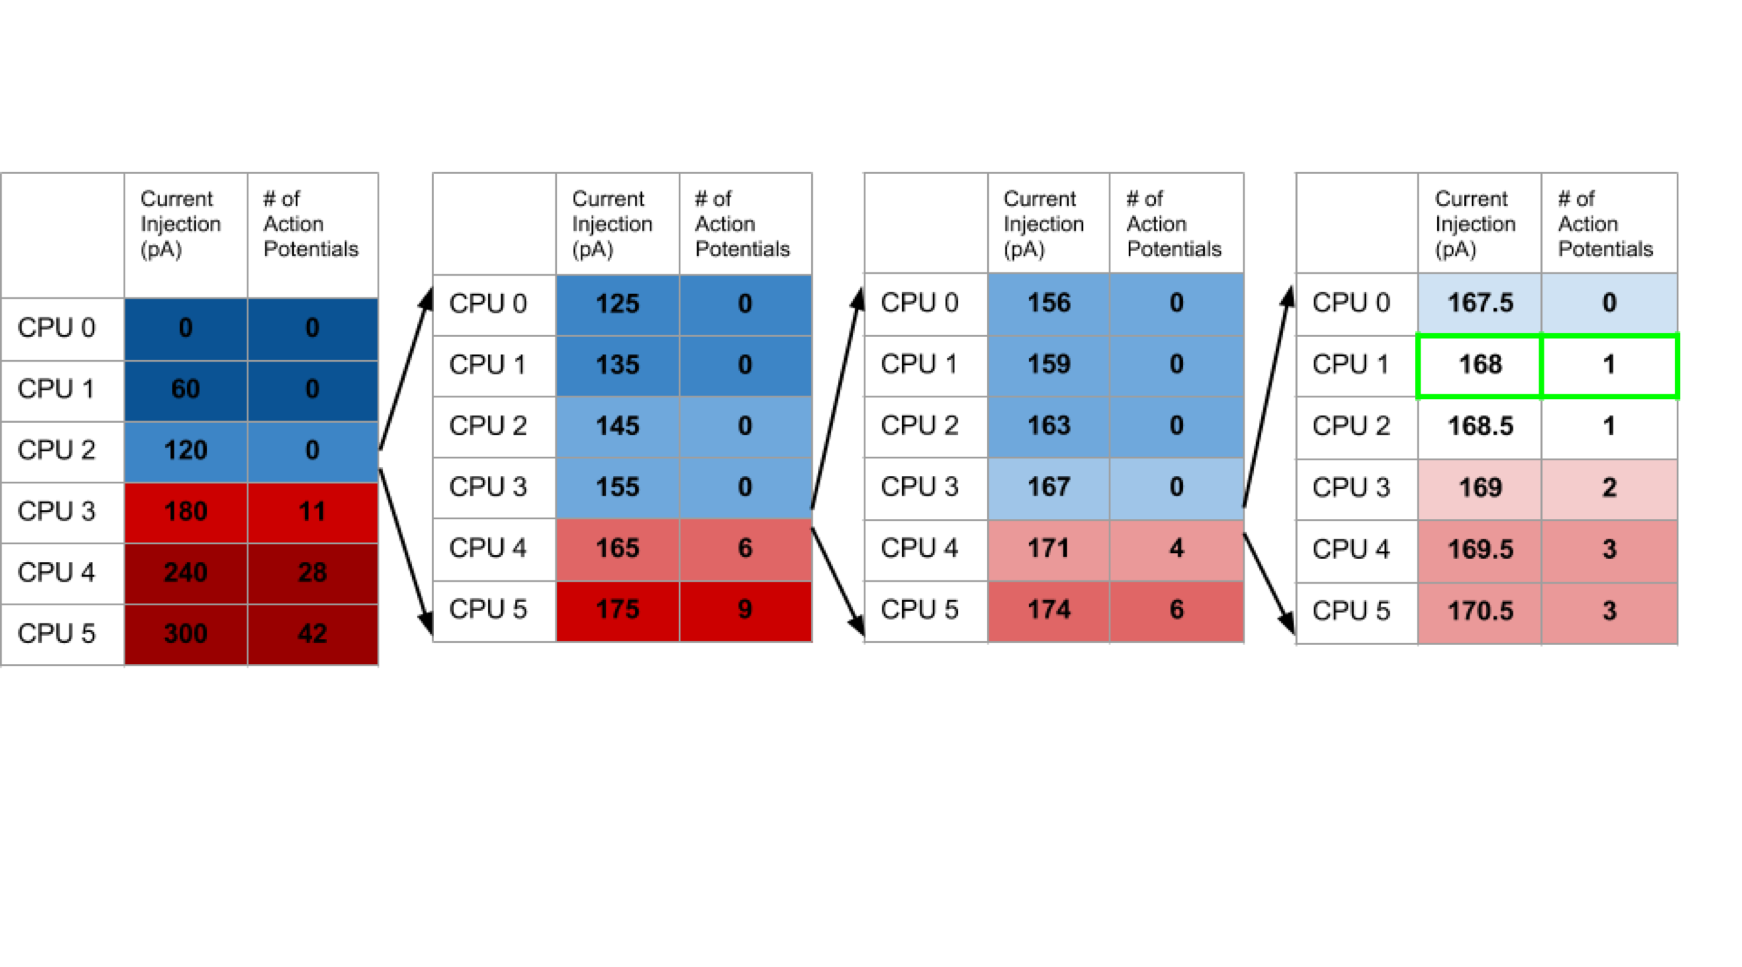
\includegraphics[width=0.7\linewidth]{{figures/rheobase_algorithm.png}}
    \caption{We developed a generic algorithm which took models, and found the minimal current injection value that would cause only one spike. The normal structure of this algorithm is a binary search, however we modified the algorithm so it would map onto multiple processors at once. This lead to significant speed ups for multicompartment NEURON models}
    \label{fig:rheobase}
  \end{center}
\end{figure} 
    
\subsection{Practical application}
I benchmarked this approach using simulations of multi-compartment neuron models.
The parallel rheobase determination algorithm resulted in a significant speed up relative to the serial algorithm.
To amplify the effect, I also considered a scenario where one wants to learn the value of the rheobase with much more precision (down to small fractions of a pA), for example in studies of dynamics in the neighborhood of a bifurcation where all other state variables can be considered nearly unchanged in the sub- and suprathreshold scenarios.
To achieve such precision, i.e. for such a small value of $i$ $0.0001*pq.fA$, the number of simulations $log_2(I/i)$ may be ~20.
Since additional model features may require only a few additional simulations to extract, it is clear that in this scenario the rheobase completely dominates the bulk of the total simulation budget.

In this scenario, using only 16 threads (with a theoretical speedup of $log_2(16+1) ~ 4.09$), I achieved the following results:
\begin{verbatim}
NEURON simulation of multicompartmental model
Serial Rheobase determination: 18.7 s
Parallel Rheobase determination: 4.8 s
Speed up = 3.9x

Brian2 simulation of AdEx model
Serial Rheobase determination: 0.791 s
Parallel Rheobase determination: 0.259 s
Speed up = 3.0x
\end{verbatim}

The total speedup approached but fell a bit short of the theoretical speedup due to overhead in the parallel search algorithm itself.
As the complexity of each simulation increases, and as the number of CPU cores brought to bear increases, this overhead should become a vanishingly small fraction of the total rheobase determination time.

\subsection{Generalization to target spike counts}
This approach determining rheobase was also generalized into a more fundamental algorithm for determining the amplitude of current required to generate a target number of action potentials.
In other words, it can be used to invert points along a models "F-I" function.
\url{https://github.com/russelljjarvis/neuronunit/blob/master/neuronunit/tests/target_spike_current.py}.

\section{Electrophysiological Measurement Distributions From the Experimental Literature}
\label{sec:data-sources}
Organized, publicly available electrophysiological measurements from single, biological neurons can form an optimization target.
Together, they can be used to parameterize a suite of tests against which a model is optimized.
Optimization aims to find model parameters so that electrophysiological measurements based on model simulations are as similar as possible to those observed in neurons.

\subsection{NeuroElectro}
\label{sec:neuroelectro}
One general source of such experimental measurements is The NeuroElectro Project \citep{tripathy2014neuroelectro}, which contains experimental values for 47 distinct electrophysiological measurements across 235 different neuron types.
As with most of the data discussed here, most (but not all) of these measurements were obtained from slice physiology experiments in rodents.
These measurements were programatically extracted from peer-reviewed journal articles over a $\sim20$ year period from $\sim1990-2012$,
and are made easy to access by an application programming interface (API) that NeuronUnit provides bindings to.
Importantly, the measured values--even for a single neuron type--reflect experiments done in many labs using (in some cases) variable methods.
Therefore, the mean of these values (e.g. the mean input resistance across reported Purkinje cells) averages over heterogeneity across cells within a slice, slices within an animal, animals within a lab, and labs within the field.
The sample size for one measure (e.g. input resistance) may be larger than for another (e.g. resting potential) meaning that these measures may reflect different subsets of experiments.
With those caveats in mind, NeuroElectro remains the most direct way to get a large number of optimization-constraining data values for most neuron types.

In order to verify that the data from NeuroElectro was plausible and was being captured correctly for the purposes of the work in this thesis, I used the API along with a batch visualization pipeline to visualize the distributions of electrophysiological measurements and inspect them for a) quality control and b) evidence of multimodality.
Multimodality, meaning multiple peaks in the histogram of a single measurement type for a single cell, could be evidence of a physiological heterogeneity not easily explained by random measurement error.
Two peaks in the histogram, for example, could result from two distinct subclasses of a single nominal neuron type, each with its own (narrower) distribution of the same measurement.
In some instances, the mean and standard deviation alone described the measurement distributions well, as would be expected for random, normally-distributed measurements of a single cell type under reasonably consistent conditions.
These values were then ``approved" for use in model-fitting.
In other cases, these conditions were not met, as exemplified in the figures below.

%\begin{comment}
%\begin{figure}
%\centering
%   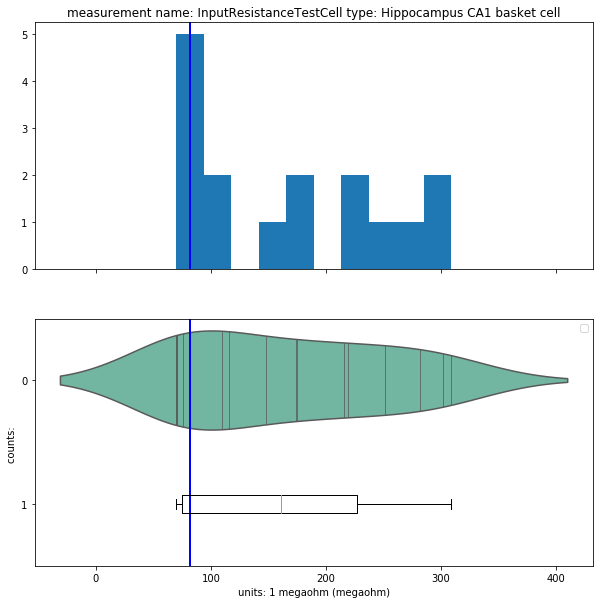
\includegraphics[scale=0.8]{notebooks_converted/needata_thesis_files/needata_thesis_5_5}
%\end{figure}

%\caption{Model parameterization of the brian2 simulator with the customization: interpolated spike height, forced to be above $0mV$}
%
%  \label{fig:sub1}
%\end{subfigure}%
%\begin{figure}
%\centering
%  \includegraphics[scale=0.8]{notebooks_converted/needata_thesis_files/needata_thesis_5_6}
%\end{figure}

%    
%    %\caption{Default model parameterization of the custom written integrator}
%  \label{fig:sub2}
%
%\begin{subfigure}
%  \centering
%      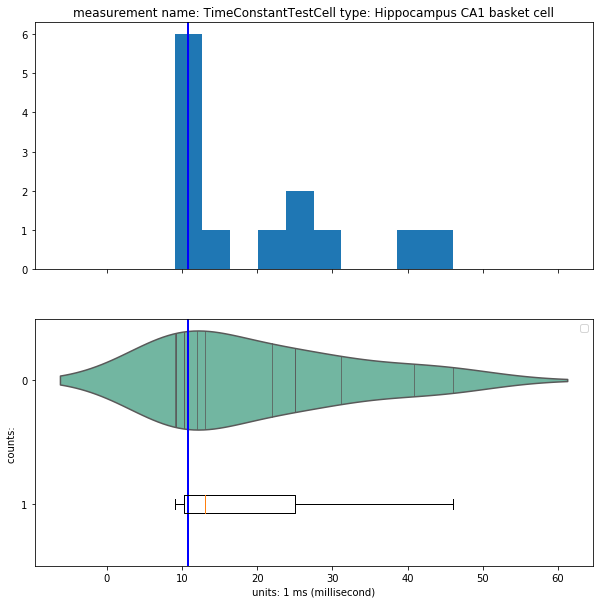
\includegraphics[scale=0.8]{notebooks_converted/needata_thesis_files/needata_thesis_5_7}
%      %\caption{Default model parameterization of the custom written integrator}
%  \label{fig:sub2}
%\end{subfigure}
%
%\caption{Comparison between two Adxaptive Exponential Implementations}
%\label{fig:test}
%\end{center}
%\end{figure}
%
%\end{comment}

%\begin{center}
%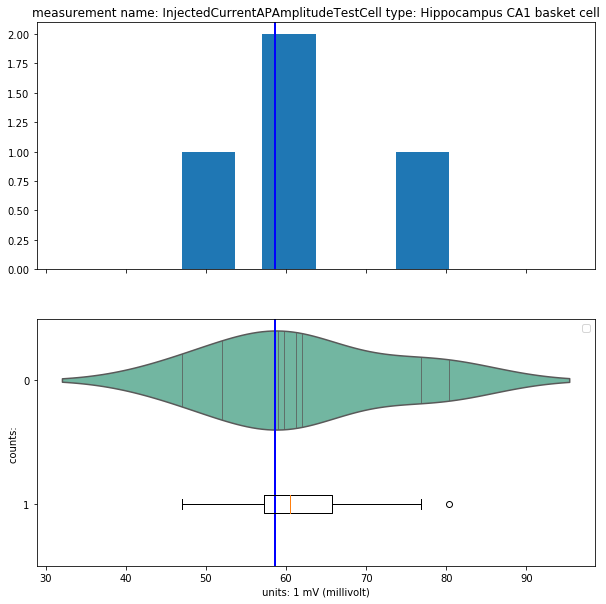
\includegraphics[width=0.7\linewidth]{notebooks_converted/needata_thesis_files/needata_thesis_5_8}
%\end{center}
%
For the majority of cell types and electrophysiological features, the distributions obtained from NeuroElectro were well-described by a normal (or log-normal) distribution.
However, I manually identified and labeled those cases where the data were not well-behaved, as these cases are likely to produce optimized models that do not reflect anything of biological relevance.

Methods for verifying that a distribution is unimodal exist \citep{maechler2013package}; however, rather than entrust this job to top-down automation, I decided to apply my own human knowledge of statistics in order to assess each distribution individually. %, because there seemed to be less opportunity to suffer from some kind of machine introduced violation of intuition. % too each  

%I achieved greater quality control through visual inspection of each case in a piece-meal manner. % manually means to do something by hand. 
I estimated that across all NeuroElectro data sampled here, about $2/3$ of distributions are well represented by a unimodal and normal distributions (e.g. Figure \ref{fig:normal-feature}).
In the remaining $1/3$, where this did not hold, I observed a small but still significant number of odd cases: highly skewed distributions (Figure \ref{fig:skewed-feature}), bimodal distributions (Figure \ref{fig:bimodal-feature}), uniform-like distributions, and distributions with insufficient samples to make any judgement.

\begin{figure} 
    \begin{center}
   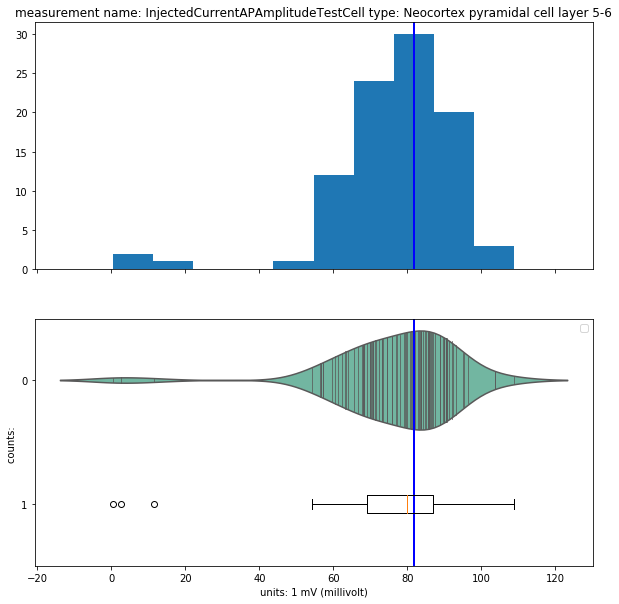
\includegraphics[scale=0.8]{figures/mean_well_served.png}
   \caption[AP Threshold Data Distribution for Layer 5 Pyramidal Cell]{\textbf{AP Threshold Data Distribution for Layer 5 Pyramidal Cell.} The majority of NeuroElectro data sets followed a normal distribution, where the mean is surrounded by a very high density of samples, which slowly thin out with increasing distance from the mean. The distribution is approximately symmetrical. Top Panel: A histogram of AP Threshold measurements from Layer 5 Pyramidal Cells; Bottom Panel: A violin plot and a box plot summarizing the same distribution. In this plot, the mean and mode are close together (a necessary condition for near-normality).
   Analagous plots were generated and inspected for all electrophysiological features computed here.}
   \label{fig:normal-feature}
    \end{center}
\end{figure}   

%\begin{figure} 
%    \begin{center}
%    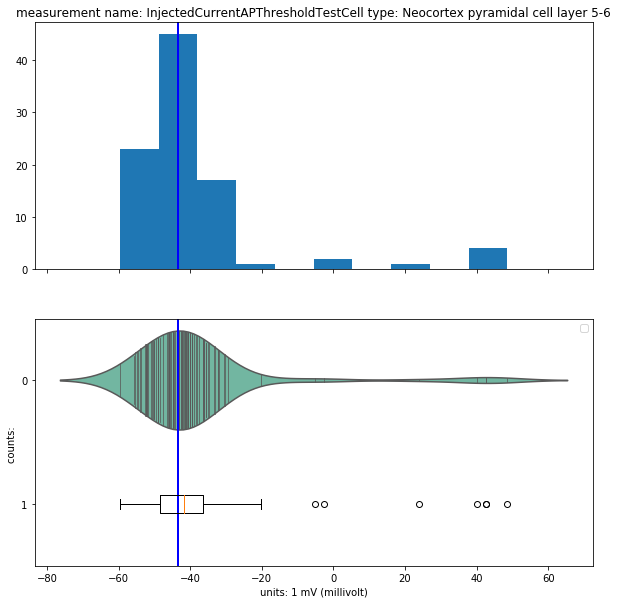
\includegraphics[scale=0.8]{figures/mean_well_served2.png}
%    \end{center}
%    \caption[AP Amplitude Data Distribution for Layer 5 Pyramidal Cell]{\textbf{AP Amplitude Data Distribution for Layer 5 Pyramidal Cell.} Same as the figure above, but for the AP Amplitude.}
%    \label{fig:normal-feature2}
%\end{figure}   
 
\begin{figure} 
    \begin{center} 
    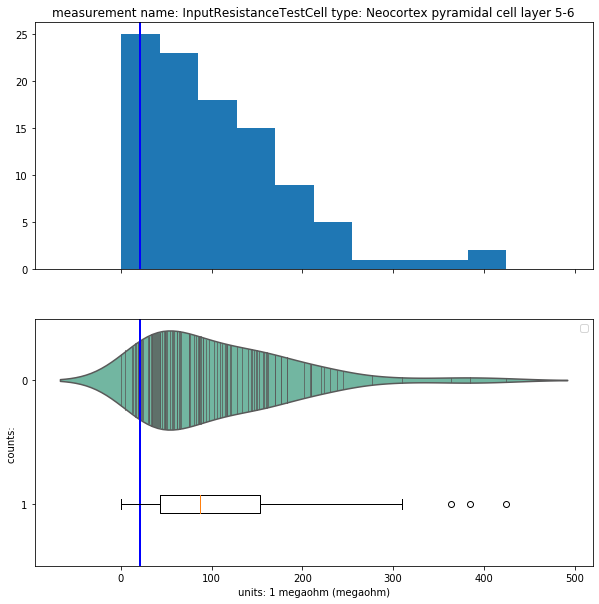
\includegraphics[scale=0.8]{figures/skewed_distribution.png}
    \end{center}
    \caption[Example of Skewed Distribution]{\textbf{Input Resistance Data Distribution for Layer 5 Pyramidal Cell.} Similar to Figure \ref{fig:normal-feature}, except for Input Resistance.
    Unlike in that figure, the distribution shows a strong skew towards higher values.
    The mean and the mode are no longer well-aligned, and therefore the mean is no longer representative of the most typical value of this feature for this neuron type.}
    \label{fig:skewed-feature}
\end{figure}   

%\begin{figure} 
%\caption[NeuroElectro data - uniform distribution]{}
%    \begin{center}
%    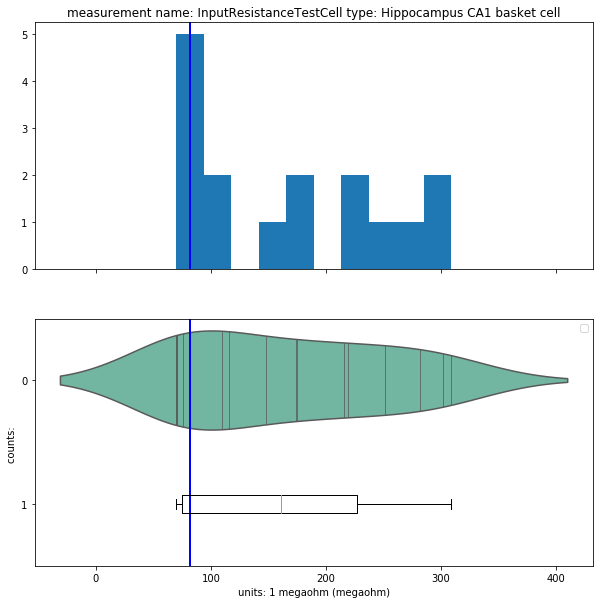
\includegraphics[scale=0.8]{figures/uniform_distribution.png}
%    \end{center}
%\end{figure}       
%%
% Neuronunit code handles under sampled neuroelectro code.
%\begin{figure} 
%\caption[NeuroElectro data - undersampled distribution]{}
%    \begin{center}
%    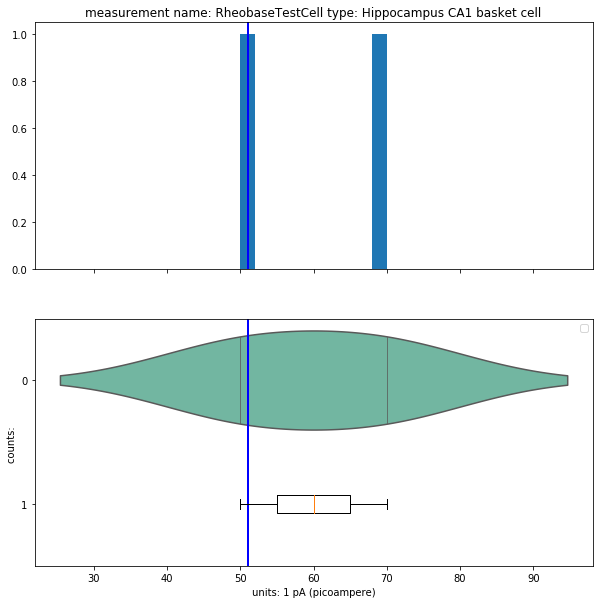
\includegraphics[scale=0.8]{figures/undersampled_distribution.png}
%    \end{center}
%\end{figure}   
%%
    
%\begin{figure} 
%    \begin{center}
%   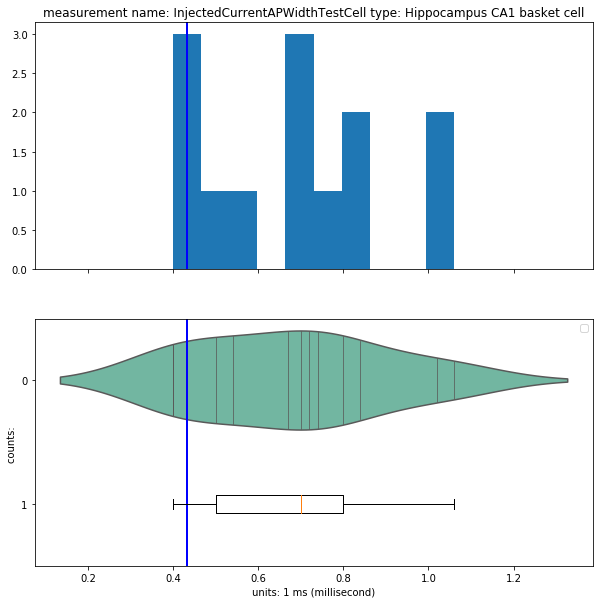
\includegraphics[scale=0.8]{chapters/notebooks_converted/needata_thesis_files/needata_thesis_5_9}
%   \caption{The Action Potential Width of the Hippocampus CA1 basket cell possibly has either an underlying uniform distribution or a multimodal distribution. Since the samples are few, the true distribution is unknown. If the distribution is uniform the gaps in the distribution, that give the histogram a multimodal appearance, as the sample size is lower enough that such gaps may only represent missing samples.}
%    \end{center}
%\end{figure}


%\begin{figure}   
%\begin{center}
%   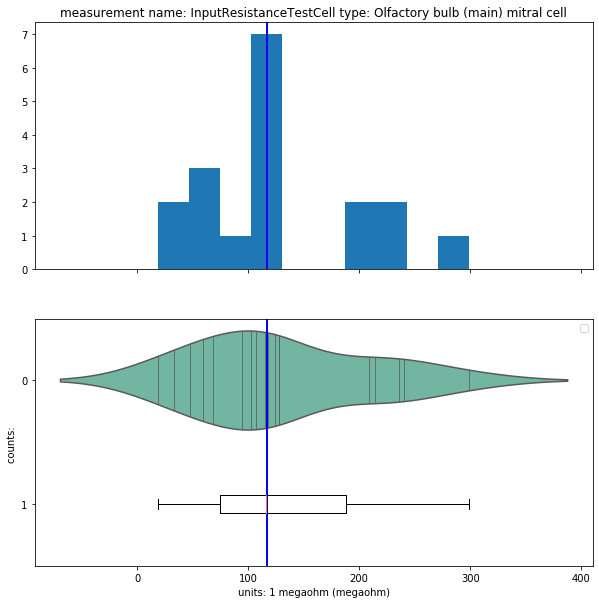
\includegraphics[scale=0.8]{chapters/notebooks_converted/needata_thesis_files/needata_thesis_5_21}
%         \caption[Input Resistance Olfactory Neuron, Perhaps Bimodal]{Input resistance of the Olfactory Mitral cell showed some tendency towards underlying bi-modal distribution, however in the second block of histogram bins, centered around $200-300pA$ only contains approximately $5$ samples. Due to a lack of samples it is also possible to conclude that the data belong to an under sampeled uniform distribution. This data set was important, as one Olfactory neuron test was constructed from this data.}
%\end{center}
%\end{figure}
   
\begin{figure}  
\begin{center}     
  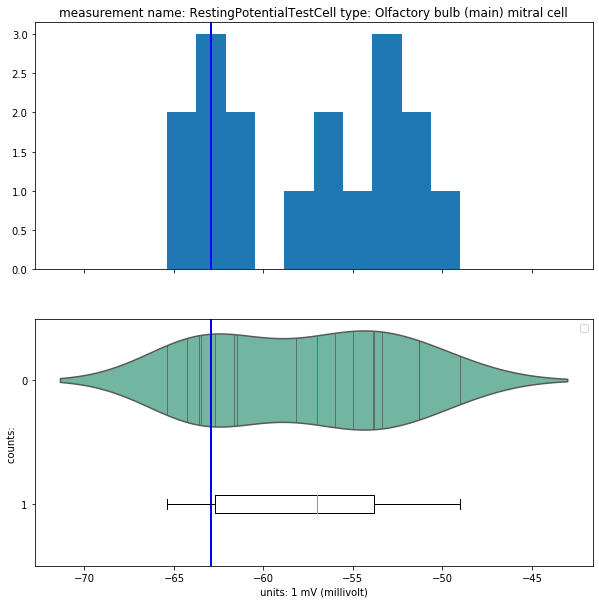
\includegraphics[scale=0.8]{chapters/notebooks_converted/needata_thesis_files/needata_thesis_5_22}
      \caption[Bi-modal Distribution for Resting Membrane Potential from Mitral Cells]{\textbf{Resting Potential Data Distribution for the Olfactory Bulb Mitral Cell.} Similar to the previous figures, but for a different cell type and electrophysiological feature.
      In this case, the distribution is clearly bimodal, with each mode containing a similar density of the data.
      Now both the mean and the median (small red line in box plot) are especially unrepresentative, lying in a region of low probabilty density.
      }
      \label{fig:bimodal-feature}
\end{center}     
\end{figure}
%%
% There are plenty of examples of bi-modal distributions in measurements from cells which are not relevant to this work.
%
%\begin{figure}
%  \centering
%  \includegraphics[scale=0.8]{chapters/notebooks_conv%erted/needata_thesis_files/needata_thesis_5_6}
%   \caption{Default model parameterization of the custom written integrator}
%  \label{fig:sub2}
%\end{figure}
%\begin{figure}
%\begin{center}
%includegraphics{chapters/notebooks_converted/needata_thesis_files/needata_thesis_5_13}
%\end{center}
%\end{figure}
    
%\begin{figure}
%\begin{center}
%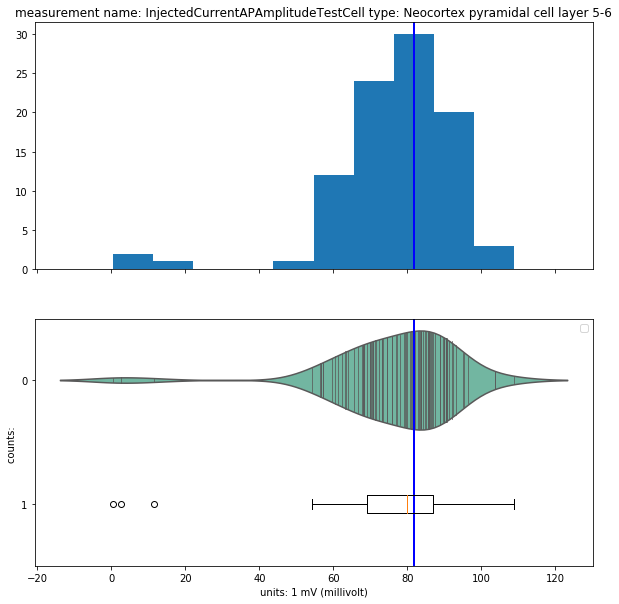
\includegraphics[width=0.7\linewidth]{chapters/notebooks_converted/needata_thesis_files/needata_thesis_5_16}
%\caption[Spike Width Measurements from Neocortical Pyramidal Neurons]{\textbf{Spike Width Measurements from Neocortical Pyramidal Neurons.} (Top Panel) Binned histogram of NeuroElectro spike width measurements from neocortical pyramidal neurons.
%The mode is denoted by the blue vertical line. The mode can be compared to the mean shown in the box plot. Often modes and means of measurements disagree.  NeuroElectro shows that a very common distribution shape is one which is possibly uniform or multi-modal. It is worth noting that a uniform distribution is not well-described by a normal distribution.}
%\label{fig:uniform-feature}
%\end{center}
%\end{figure}

%\begin{figure}
%\begin{center}
%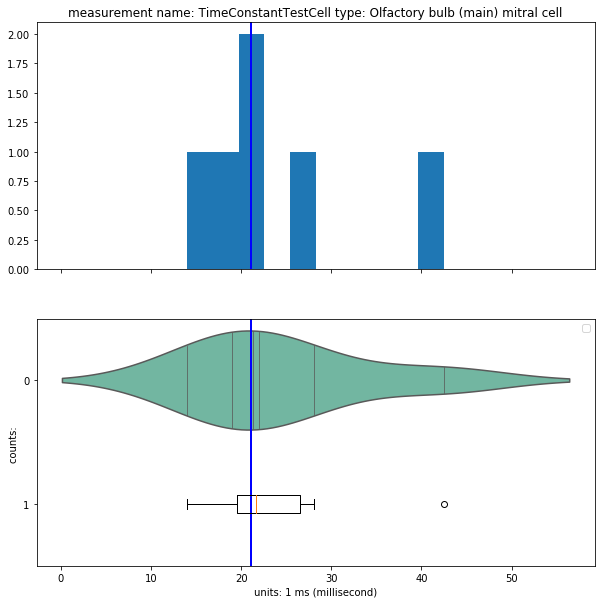
\includegraphics[scale=0.8]{chapters/notebooks_converted/needata_thesis_files/needata_thesis_5_23}
%\caption{Similar to the figure above, but for a different neuron type.}
%\label{fig:uniform-feature2}
%\end{center}
%\end{figure}

\subsection{EFEL and The Allen Institute Cell Types Database}
The Electrophysiology Feature Extraction Library (EFEL) \citep{EFEL} was developed as part of the Blue Brain Project. Although EFEL computes common spike train statistics related to spike timing, approximately 2/3rds of features extracted by EFEL pertain to spike shape, where some of these features are shown below. 
The Allen SDK comes with a very comprehensive Python-based feature extraction suite. Like EFEL, the Allen suite well-represents a large number of spike shape measurements as well as spike train statistics. 
Unfortunately, the Allen SDK feature extractor is significantly slower than EFEL, as EFEL was implemented using the very fast language $C++$. The performance cost may not be felt when dispatching single runs, but slow performance is a significant impediment to optimization. 
In optimisation, feature extraction is directly coupled to chromosome fitness calculations, and it is executed very often across the evolution of the genetic algorithm. Additionally by default, the Allen SDK feature extractor assumes that the user will apply very high sample frequency and noisy traces encoded in the NeuronData Without Borders \citep{teeters2015neurodata} standardized format. 
These traces require filtering before computing the Allen features, where significant intervention is required to turn off filtering. 
Inappropriately applying filtering to model traces causes problems, because the the lower sampling frequency intrinsic to simulated model traces is not predicted by the digital filter. Overall, the EFEL was fast enough to be useful, and its default settings were appropriate to my use case \citep{garcia2014neo}.

Data available through NeuroElectro cover a large number of cell types; however, recording conditions and measurement algorithms are heterogeneous.
It is unclear whether the distribution of measurements across such an ensemble is actually a good summary of any one individual neuron.
In order to ensure that reduced models could be optimized against data recorded exclusively from single neurons, I also used data from the Allen Institute Cell Types Database \citep{celltypes}, a project of the Allen Institute for Brain Science.
This Cell Types database consists of summary physiological, morphological, and histological data for thousands of individual neurons (across a few dozen subtypes) from mouse visual cortex, obtained using patch clamp recordings in slices.
Each experiment is done using exactly the same methods and with the same sequence of stimuli \citep{celltypes}, ensuring not only that models generated using this data are directly comparable, but that each such model is reflective of an individual neuron.

The Cell Types Database provides some limited pre-computed measures of action potential waveform characteristics. 
However, the data are not organized in a way that makes it is useful for the types of optimization and data analysis performed here.
Specifically, I require features that are computed on cell responses to current injection values that are fixed multiples of rheobase.
Additionally, the pre-computed features are thin relative to those that used for the optimizations described in the Results section.
Because raw data are available through the Cell Types API, I re-computed all necessary features from this raw data, according to the consistent standards reflected in the NeuronUnit code.

In contrast to NeuroElectro, the Cell Types database also has a great deal more information relevant to the above threshold dynamics of neurons, such as the number and pattern of action potentials they discharge in response to somatically-injected currents much larger than rheobase, or in response to non-square injected currents.
In order to exploit these, I developed several additional NeuronUnit tests using EFEL (describe later in sections \ref{sec:efel}), such as: ``time to first spike test", ``mean AP amplitude test", ``time to last spike test" and ``adaption index". In principal any feature measured in the Cell Types Data could be upgraded to a NeuronUnit test, and I created a code-generation template to accelerate this task. Effectively, code generation meant, that any EFEL feature, could be turned into a NeuronUnit test. In principle Allen tests can be generated from templates in much the same way. The final set of operational tests
were EFEL \cite{EFEL} tests that were adapted from descriptions of feature extraction in the literature and shown in Table \ref{tab:features}. 
Features are shown in Figures \ref{fig:voltage_figures} and \ref{fig:features_example}.
I also crafted additional NeuronUnit tests to supplement these including one that measures the slope of the FI curve ($FISlopeTest$) and one that measures the coefficient of variation of the ISI distribution for suprathresholds stimuli ($ISICVTest$), a measure of burstiness. 
%%
% \ref{sec:allensdk},
% Allen are features, not tests (no judge methods).
% currently, its very transient.
% Allen used to be tests, it was hard to % maintain code. 

%%%
% Tests I rewrote from scratch 
% not EFEL, was FITest, CVTest, ISITest
%%%


%\begin{figure}
%\centering
%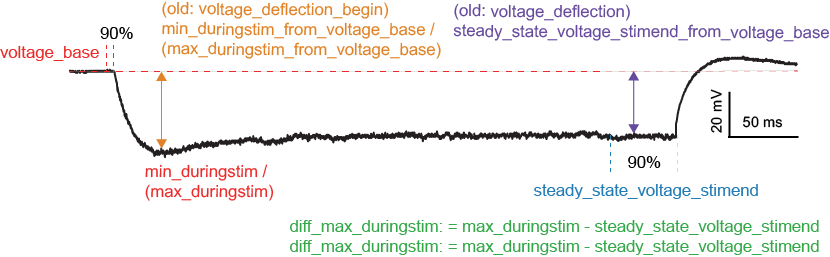
\includegraphics{figures/voltage_features.png}
%\caption[Passive Membrane Properties Measured from a Hyperpolarizing Current Stimulus]{\textbf{Passive Membrane Properties from a Hyperpolarizing Stimulus.} Applying a negative (outward, hyperpolarizing) current stimulus minimially activates voltage-dependent ion channels, making it a good method for measuring ``passive" membrane properties such as the input resistance (measured as the difference between the resting potential (red) and steady-state hyperolarization (blue).
%Nonetheless, some intrinsic conductances are activated, allowing for measurment of additional features such as the sag ratio (red trough vs blue steady state). Figure from EFEL documentation \url{https://efel.readthedocs.io/en/latest/eFeatures.html}.}
%\label{fig:voltage_figures}
%\end{figure}

\begin{figure}
\begin{center}
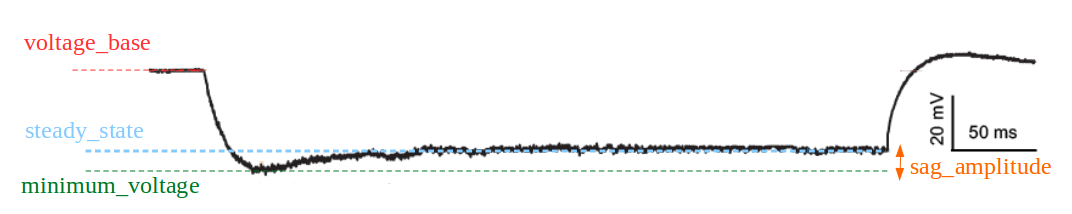
\includegraphics{figures/sag_amplitude}
\end{center}
\caption[Passive Membrane Properties Measured from a Hyperpolarizing Current Stimulus]{\textbf{Passive Membrane Properties from a Hyperpolarizing Stimulus.} Applying a negative (outward, hyperpolarizing) current stimulus minimially activates voltage-dependent ion channels, making it a good method for measuring ``passive" membrane properties such as the input resistance (measured as the difference between the resting potential (red) and steady-state hyperpolarization (green).
Nonetheless, some intrinsic conductances are activated, allowing for measurment of additional features such as the sag amplitude or ratio (green trough vs blue steady state). Figure from EFEL documentation \citep{efel-docs}.}
\label{fig:voltage_figures}
\end{figure}

\begin{figure}
\centering
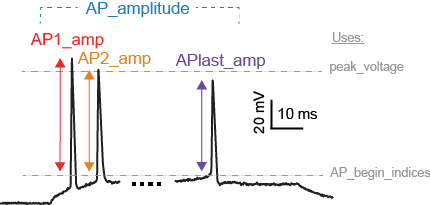
\includegraphics{figures/AP_Amplitude.png}
\caption[Action Potential Features Measured from a Depolarizing Current Stimulus]{\textbf{Action Potential Features Measured from a Depolarizing Current Stimulus.} A positive (depolarizing, inward) current of sufficiently amplitude produces one or more action poentials.
Many features can be computed from these, including their absolute amplitudes (in color), relative amplitudes, widths, thresholds, and afterhyperpolarizations (AHPs).
Additional features about their number and relative timing can also be computed (not shown).
Figure from EFEL documentation \citep{efel_documentation}.}
\label{fig:features_example}
\end{figure}



%XXXX Russell, can you list the new tests above.

These tests can be used to assess the agreement between neuron models and biological neurons on supra-threshold dynamics, largely reflected in patterns of spiking such as bursting and adaptation, but also mean spike height and mean spike width, resting membrane potential, mean trough depth, and upstroke times.

\subsection{The Blue Brain Project Neocortical Microcircuit Portal}
\label{sec:bluebrain-data}
I also made use of an additional data source, the The Blue Brain Project Neocortical Microcircuit Portal, similar in some ways to the Allen Institute Cell Types Database but reflecting measurements taken from mouse somatosensory cortex (again in patch-clamp recordings from slices).
From this dataset I exclusively used a collection of experiments from animal $B95$, which for reasons unknown yielded a tremendous amount of data \citep{ramaswamy2015neocortical}.
Conceptually, this dataset did not add anything new, but it did allow for high-quality optimized models to be produced from another brain region (somatosensory, rather than visual cortex).
These data are also linked to--and constrain--the on-going Human Brain Project effort to simulate biophysically-detailed multi-compartmental models of the same neurons (and whole neural circuits).
This means that the reduced models produced here can be compared directly to those more detailed models, or that the general NeuronUnit-driven genetic optimization framework developed here could be used to optimize detailed models which should, in principle, be similar to those produced through the larger Human Brain Project effort.
Indeed, the Human Brain Project is already a user of the SciUnit framework developed in my lab, on which NeuronUnit is based.

\begin{table}
\centering

\resizebox{\textwidth}{!}{
\begin{tabular}{|l|l|}
            \toprule
            \textbf{Test Name} & \textbf{Test Description}\\
\midrule
adaptation-index & Measures spiking fatigue in response to constant current\\
 adaptation-index2 & The same as Adaption index1, except it is used as an alternative when spikes below $0mV$ occur.   \\
time-to-first-spike & amount of time elapsed until first spike \\ mean-AP-amplitude & The average spike height in a spike train \\
spike-half-width & The width of a spike is obtained at point when spike height is half its total amplitude\\    
AHP-depth & The after hyperpolarisation depth\\
minimum-voltage & The minimum voltage\\
peak-voltage & the maximum voltage, usually a spike peak. \\
time-to-last-spike & The time of last spike onset \\
AHP-depth-abs & After Hyperpolarisation depth (absolute value).\\
all-ISI-values & All interspike interval times\\
voltage-base & minimum voltage while undergoing stimulus, often below the threshold of APs. \\
min-voltage-between-spikes & Needed because during  high frequency firing AHPs may be skipped.\\
Spikecount & Just the number of spikes that occured in the provided stimulus window\\
\bottomrule
\end{tabular}}
\caption[List of EFEL Features]{14 key features identified in the EFEL \citep{EFEL} library that I impemented and encoded into NeuronUnit tests for optimization.}
\label{tab:features}
\end{table}

% There is no "NeuronUnit" data. What does this mean?
The tests which lead to the best fits in the above threshold experiments were the tests made from application of EFEL features to Allen data sources (Figure \ref{fig:voltage_figures}). The measurement type and the test type did not change between Allen Cell Types and Blue Brain Data. Only the reference data which informed comparison measurements changed. % \ref{fig:supra-threshold-tests})

Table \ref{tab:features} constitutes a summary of both NeuroElectro and Allen experimental data reports. %This data can naturally be reported in tabular form. 

%\subsection{Experimental Measurements}

\begin{table}[ht]
\centering
\resizebox{\textwidth}{!}{
\begin{tabular}{|l|l|l|l|l|l|l|l|l|}
\toprule
Test Name / Cell Type & CA1 Pyramidal & Purkinje & NCP Layer 5-6 &      Mitral Cell & 623960880 & 623893177 & 471819401 & 482493761 \\
\midrule
RheobaseTest                   &                      189.24 pA &                680.79 pA &                          213.85 pA &          NaN &        70.0 pA &       190.0 pA &       190.0 pA &        70.0 pA \\
InputResistanceTest            &                    107.08 $M\Omega$ &              142.06 $M\Omega$ &                        120.67 $M\Omega$ &  130.08 $M\Omega$ &  241.0 $M\Omega$ &  136.0 $M\Omega$ &  132.0 $M\Omega$ &  132.0 $M\Omega$ \\
TimeConstantTest               &                        24.5 ms &                      NaN &                           15.73 ms &     24.48 ms &        23.8 ms &        27.8 ms &        13.8 ms &        24.4 ms \\
CapacitanceTest                &                        89.8 pF &                620.27 pF &                          150.58 pF &    235.75 pF &            NaN &            NaN &            NaN &            NaN \\
RestingPotentialTest           &                      -65.23 mV &                -61.59 mV &                          -68.25 mV &    -58.14 mV &       -65.1 mV &       -77.0 mV &       -77.5 mV &       -71.6 mV \\
InjectedCurrentAPWidthTest     &                        1.32 ms &                  0.41 ms &                            1.21 ms &      1.61 ms &            NaN &            NaN &            NaN &            NaN \\
InjectedCurrentAPAmplitudeTest &                       86.36 mV &                 71.23 mV &                           80.44 mV &      68.4 mV &            NaN &            NaN &            NaN &            NaN \\
InjectedCurrentAPThresholdTest &                       -47.6 mV &                -46.89 mV &                          -42.74 mV &     -38.9 mV &            NaN &            NaN &            NaN &            NaN \\
FISlopeTest                         &                            NaN &                      NaN &                         0.05 Hz/pA &          NaN &     0.18 Hz/pA &     0.12 Hz/pA &     0.18 Hz/pA &     0.09 Hz/pA \\
\bottomrule
\end{tabular}}
\caption[Neuroelectro Data]{Data for 9 tests (features) across 8 cells.
The first 4 cells are specific cell types spanning several brain regions, and the corresponding data comes from neuroelectro.org.
The remaining 4 are single (cortical) cells comes from the Allen Cell Types database, and the features were directly computed using NeuronUnit tests.
``NCP" indicates neocortical pyramidal.}
\label{tab:neuroelectro-data}
\end{table}


\subsection{Novel Data-Driven Tests for Model Optimization}
At the onset of this project, NeuronUnit contained a range of model validation tests, but these were inadequate for for optimization.
Most such tests were restricted to measurements of passive membrane properties or action potential waveforms.
However, the rich diversity of neuronal physiology is also reflected in the rate, timing, and sensitivity of patterns of action potentials.

As noted in Section \ref{sec:data-sources} there where two experimental data types, each of which was used to constrain models differently: raw data from which features were (re-)calculated, and pre-computed features as reported in the literature.
The distinction is important here because in the former case new feature extraction routines are required.
In order to developed tests based on these newly calculated features, I created an interface to the Allen Cell Types API; this allowed me to automatically create NeuronUnit tests parameterized by features extracted from the membrane potential traces available from the Allen Institute through that API.
In order to create the new NeuronUnit tests, one must query the Cell Types Database, impose a new organization on the data, extract relevant features, and convert model features for use with NeuronUnit tests.
A similar API was created in order to work with the Blue Brain data described in section \ref{sec:bluebrain-data}, so that both of these data sources could then guide model fitting.
These APIs and their use in generating NeuronUnit tests are documented in \url{https://github.com/fun-zoological-computing/BluePyOpt/blob/master/examples/bpo_nu_fusion/allen_efel_nu_deployed_tests_only-thesis.ipynb}

At this stage the range of tests available for optimization in NeuronUnit was still incomplete; the data was adequate, but several key features that distinguish one pattern of spiking from another were still missing. Therefore, I implemented another series of tests in NeuronUnit using the EFEL features (section \ref{sec:efel}).
I developed the ability for all of the EFEL features to be calculated on NeuronUnit models, as well as a new test to compute the slope of the F-I curve.
I organized these tests into new "at threshold" and suprathreshold test suites, which included features such as
interspike-interval (ISI) statistics, after-hyperpolarization (AHP) depths, spike frequency adaption ratios, etc.
For example, I utilized an existing implementation of the spike frequency adaptation index. The adaptation index is calculated as follows \citep{EFEL}:

\begin{equation}
A = \frac{1}{N - k - 1} \sum_{i = k}^N \frac{isi_i - isi_{i-1}}{isi_i + isi_{i-1}}
  = \frac{1}{N - k - 1} \sum_{i = k}^N \frac{tpeak_{i+1} - 2 tpeak_i + tpeak_{i-1}}{tpeak_{i+1} - tpeak_{i-1}}
\end{equation}
where the first $k$ peaks are skipped and:
\begin{align}
    \textrm{the interspike intervals:    } & isi_i = tpeak_{i+1} - tpeak_i,
    \textrm{the number of peaks:    } & N.
\end{align}
%The parameter \verbatim{spike skipf} is the fraction of skipped peaks, $k$ is %the minimum of \verbatim{spike skipf} times $N$ and \verbatim{max spike skip}.
  

In order to optimize reduced models, it was necessary to develop ``optimizer-friendly" implementations of these models.
As described in section \ref{sec:new-models}, I developed three different optimizer-friendly reduced models: the Izhikevich model (spanning seven dynamical regimes), the Adaptive Exponential Integrate and Fire (AdEx) model, and the GLIF model.
Additionally I created one slower single-compartment conductance-based model and I retrofitted a pre-existing multi-compartment conductance based model to make a broader array of comparisons across model types.

\subsection{Conversion Between Types and Model Exchange Across Threads}
Multi-core and or multi-threaded optimization requires that information about model properties be shareable across various processor threads.
However, some very common data types used in programming are not easily shareable between CPUs.
The release of Python 3.8 solved a subset of these problems, but this did not occur until late 2019 so I implemented an alternative scheme for cross-thread sharing of models.
I created a new NeuronUnit class ``Data Transport Container", whose main function was to circulate essential data about model parameters and state variables between threads.
Models on one thread were collapsed into this container, shared between threads, and then reconstituted on a new thread.
This added a small amount of overhead, but this computational cost was negligibly small when measured against the gains of using multi-threaded processing.

Outside of multi-threading context the DTC class should be conceptualized as an essential expansion to Neuronunit base model class which allows the optimization of Neuronunit models. The DTC class makes it possible to do many common genetic algorithm operations ``in place". It enables the creation chromosomes from any existing model, to evaluate the fitness of any single chromosomes, and to convert chromosomes back to models. The DTC type is able to evaluate most feature extraction algorithms on itself. Many users of NeuronUnit, are not performing optimization, such that placing these conversions in the Neuronunit base Model class does not make sense.

%In addition to sharing essential information, across threads. The class DataTC containers role includes performing common in-place conversions and computations. 

%doing away with the DTC type would render most of the optimization code unusable.


% 

\subsection{Web Application for Optimization}
In order to both control optimization parameters and visualize optimization results, I also developed a web application that requires no programming skill to use, and allows a user to select among multiple cell-specific constraints, and multiple model types.
Once the user has specified enough parameters to define an optimization job, the job can launch, and return interactive results to the user after the optimization job completes (typically in minutes).
This is described in section \ref{sec:web-app}.
\section{Technical Details of the Optimizer}
\label{sec:tech-details}
The sections above describe my innovations in model construction and simulation, as well as the experimental data brought to bear on optimization. These data are used to parameterize NeuronUnit tests, one per measurement type.
For example, input resistance data for one neuron type in NeuroElectro, or one specific neuron in the Cell Types database, is passed to an \textit{InputResistanceTest} defined in NeuronUnit.
This test ``asks" the model to generate a corresponding simulation, measures the input resistance in this simulation output, and then assesses model/data agreement, resulting in a score.
These mechanics have been described at length previously in \cite{omar2014collaborative}, \cite{gerkin_neuronunit}, and \cite{birgiolas2019towards}.

\subsection{Generating and Using Scores}
\begin{figure}
\begin{center}
    \includegraphics{figures/normal_distribution}
    \caption[Z-scores for NeuronUnit Tests]{\textbf{Z-scores for NeuronUnit Tests}. As discussed in the section \ref{sec:neuronunit}, error functions were evaluated with the assistance of the \emph{NeuronUnit} library.
    This involves obtaining an experimental distribution over electrophysiology feature measurements for a cell type, measuring corresponding model output features, and then locating those features in that experimental distribution. 
    Scores that are closer to the experimental mean are identified as low error.
	The Z-score encodes this information; a Z-score of 0 is the lowest possible error.}
	\label{fig:normal-dist}
\end{center}
\end{figure}
%XXXX Something about Z-score vs RatioScore.

One way to ask whether the simulated feature is a good match to the biological data distribution is to use a Z-score.
The Z-score is defined as:
\begin{equation}
Z-Score = \frac{s - b_{\mu}}{b_{\sigma}}
\end{equation}
where $s$ is the value of the feature in the model simulation, and $b_{\mu}$ and $b_{\sigma}$ are the mean and standard deviation of that feature in the biological data distribution.
The Z-score does not specifically assume that the biological data are normally distributed, although this generates the most natural interpretations.
%(Figure \ref{fig:normal-dist}).
In cases when the biological data from one neuron type comes from a single experiment on a single neuron (as with some data from the Allen Cell Types database or the Blue Brain Project), there is no mean or standard deviation, so I compute a \emph{RatioScore}:
\begin{equation}
Ratio-Score = \frac{s}{b}
\end{equation}%%%Fixed error
where $b$ is the observed biological feature value.
Both types of scores were then normalized to produce an error signal in the range $(0, \inf)$ for use by the optimizer.
For example, suppose a feature(e.g. the rheobase current) had value $\mu \pm \sigma = (100pA \pm 40pA)$ in the biological data, and $110 pA$ in the simulated model output.
Then the following steps were taken to transform it into an error signal:
\begin{enumerate}
 \item A Z-score is computed: $\frac{110 pA - 100 pA}{40 pA} = 0.25$
 \item This is converted to the range (0, 1) using the error function: $abs(erf(Z)) = 0.27$ 
 \item The logarithm is computed: $\log_{10}(0.27) = 0.56$ 
\end{enumerate}
The value 0.56 above represents a larger model/data disagreement than the ``best" possible value of 0 (corresponding to a Z-score of 0), but less disagreement then the ``worst" possible value of $\inf$ (truncated in practice at 100) representing a Z-score of $+\infty$ or $-\infty$. The summed error signal over all $n$ NeuronUnit tests (e.g. rheobase, input resistance, spike rate adaptation, etc.) is:
\begin{equation}
Total  Error = \sum_i^n error_i
\end{equation}
i.e. the sum of all of the errors.  Again, 0 would represent perfect model/data agreement across all tests.

While the optimizer attempts to minimize the total error of the model according to the equation above, evaluation of the quality of the optimized model is evaluated using a hypothesis testing framework.
Specifically, I ask whether there is sufficient evidence that the optimized model is representative of the distribution of feature values observed in the biological data.
The null hypothesis can be states as ``the observed features of the optimized model were drawn from the distribution of features of biological neurons".
In order to generate a test statistic for hypothesis testing, I compute $\chi^{2}$, defined as (in the case of Z-scores):
\begin{equation}
\chi^{2}=\sum\limits_{i=1}^{n}(Z_{i}^{2})
\end{equation}
This equation arises from the fact that a Z-score is simply a standardized normal variable, and a chi-squared distribution with $n$ degrees of freedom is simply the distribution of $n$ independent, squared normal variables.
I compute a p-value by comparing the observed $chi^2$ statistic to the cumulative distribution function of the $chi^2$ distribution with degrees of freedom equal to the number of NeuronUnit tests used (which is equal to the number of Z-scores produced).
If this p-value is small (e.g. $<0.05$), that can serve as evidence to reject the null hypothesis, indicating that the optimized model did not ``fit in" well with the observed biological data.
In contrast, failure to reject the null hypothesis would suggests that the optimized model was somewhat convincing in its mimicry of a biological neuron, for the features in question.

\subsection{Mechanics of Optimization using NeuronUnit}
Here I will describe how I generate these scores concurrently for many parameterizations of the same model and how they guide the optimization path.
I created two different optimization code bases based on the DEAP Python package for genetic optimization \citep{DEAP_JMLR2012}, one that relied on DEAP directly, and one that relied on the BluePyOpt package produced by The Human Brain Project \citep{bluepyopt} (These have since been merged together), in order to achieve optimization using NeuronUnit.
A few key modules are essential to both approaches.
I wrote the file \emph{optimization-management.py} to contain the logic of and methods for managing complex optimization jobs.
It helps the optimizer handle both fixed and varying  model parameters, contains methods for random sampling of model parameter spaces, can plot models output for visualization of this space, and assists in computing the F-I curve.
I also add several methods for inter-converting between representations of the models themselves and the chromosomes that represent only parameter values.

A created a \emph{NUFeature\_standard\_suite} class to convert NeuronUnit features to BluePyOpt objective functions, as outlined in simpler terms in the enumerated list above.
These classes contain a complicated nesting of fault handling statements, as there are many reasons why a candidate model could return unusable simulation output (typically non-biological parameter values), resulting in values like $NaN$ and $\inf$; such values must be recast as poor but finite errors so that the optimizer can see a smooth error surface.
There are two flavors of \emph{NUFeature\_standard\_suite}, one for supra-threshold simulation experiments and another for at threshold or sub-threshold experiments, since each experiment type produces different feature requiring different feature extractors, and producing different sets of edge cases to be handled independently.
For example, there are more ways for a model to fail to elicit multiple action potentials (causing all ISI-based feature extraction functions to return $NaN$ values), than there are to fail to exhibit a hyperpolarizing response to a small outward current injection for the measurement of input resistance.
 
I created a \emph{model-parameters.py} file, a collection of ordered dictionaries, that informed the optimizer which parameters should be modifiable (in the highest-dimensional cases, all of them) and what are reasonable (biologically plausible) search boundaries.
This file also contains example parameter sets representing notable dynamical regimes, such as those shown in \cite{izhikevich2003simple}.
I also made this file and its methods inter-operable with BluePyOpt model parameter management scheme.

\subsubsection{Optimization Parameters}
Optimization requires searching for better and better solution across multiple generations of chromosomes (parameter sets), as noted in section \ref{sec:genetic-algorithms}.
Robust optimization for the models used here required $NGEN\sim150$ generations with a population size (number of parameter sets explored in each generation) of $\mu=35$.
In other words, it took about $150$ generations of mutation, crossover, and selection to achieve convergence, and in each generation about $35$ models had each of their feautures computed and scored.
These parameter values achieved an acceptable balance between exploration of the parameter space and exploitation of favorable regions.
In some cases, values as small as $NGEN=10$ and $\mu=10$ were tolerable, for example when optimizing only low-dimensional cross-sections of parameter space.
In other cases, such as when the number of optimization objectives (i.e. the number of electrophysiological features being tested) was $NOBJ>25$, values as high as $NGEN=300$ and $\mu=100$ were required to obtain adequate results.

\subsubsection{Multiobjective Scoring and Selection}
One potential scientific goal is to maintain a diverse set of solutions (i.e. very different parameter sets that nonetheless each produce simulations that adequately match observed experimental measurements).
The optimization literature has developed many competing approaches for doing this \citep{deb2000fast}, but it usually involves two popular algorithms, named IBEA and NSGA2, which I investigated here.
NSGA2 uses some additional ranking mechanisms, to re-weight the perceived fitness of each chromosome and influence the probability that it survives (or is bred into) the next generation.
For example, it tries to minimize ``crowding distance", penalizing chromosomes that aggregate in clusters, as persistent cluster formation means that the GA becomes preoccupied with more limited regions of the solution space, harming solution diversity.
Another meta-constraint called ``non-dominated sorting" ranks most highly each chromosomes that is not unanimously defeated by any other chromosome on any feature score.
For example, though one parameter set $P$ might produce a model which score poorly on all features except Input Resistance, if no other parameter set has a higher-scoring Input Resistance feature then $P$ is retained. Consistent with personal communication with \cite{van2007neurofitter}, adding in crowding distance and non-dominated sorting typically harms optimizer performance, in the context of neuronal model optimization, though the reason for this is not argued conclusively, I speculate on a likely cause in the discussion of this work.
A simpler ``select best" algorithm (labelled IBEA) dispenses with these tricks, performs no meta-constraint scoring, and simply retains the fittest chromosomes for mutation, crossover, and selection. This simpler selection algorithm was found to work well when optimizing reduced neuronal models.

\subsection{Comparison to Previous Approaches to Optimization}

\subsubsection{Time-dependent Mutation}
Other labs have previously developed schemes to optimize neuron models, e.g. \cite{druckmann2007novel}.
I retained the conceptual insights of these approaches where they were useful for the problems at hand.
For example, I utilized a time-dependent mutation magnitude ($\eta$).
The idea is that big mutations are more helpful in the early stage of optimization, when it is important to explore the vast hyper-volume of parameter sets and get a general picture of the error surface, and that these mutations should be smaller during the later ``refinement" stage of optimization, as the best solutions are approached. Time diminishing $\eta$ did improve genetic algorithm on reduced model optimization problems.

\subsubsection{Variants on Somatic Current Injection}
Nearly all neuron optimization work (including this one) relies on the responses to somatically-injected current as the domain for optimization.
This is largely motivated by the existence of a common and simple experimental analogue using patch clamp (which drives experimental design for both the Allen Cell Types Database and The Blue Brain Project).
But there are three different strategies for choosing the subset of these experiments that are recapitulated in optimization.

% The first strategy was to assume that measurements of an at threshold rheobase spike were sufficient to fit the model to the entire F-I curve, and if all neurons showed an identical regular, non-accommodating spiking pattern, this strategy would might be sufficient to identify a model, with all the right at threshold and above threshold dynamics. To the extent that this assumption is violated, various additional above-threshold current injections will be needed, these are described in strategies two and three. 

% The second strategy involves first identifying the rheobase currents per model and choosing two extra multiples of rheobase current reserved for further model evaluation. This strategy is more direct and slightly more rapid, but it is inefficient in terms of constraining the model, because all of the "action" in the F-I curve occurs above rheobase, but not too far above rheobase (i.e. not at currents that induce depolarization block).

% The third strategy is like the second, but deliberately samples single above threshold locations on the F-I curve (any location that elicits one spike). It is actually the third strategy that was used to produce multi spiking fits, in this work. 

% The fourth strategy involves making an informed guess to make a fixed set of current amplitudes (e.g. ascending 100 pA steps) from the data and probing the model with these, then comparing model and data within this subset. 

%Here I have described four different strategies for constraining models, 
In the optimization framework I tested many different strategies for constraining models with current injections, there were only two important differences between all four strategies: one type of strategy constrains cell behavior at multiple values of current injection, and the other strategy constrains cell behavior at a single current injection value (rheobase or otherwise). Each strategy seeks to resolve a ``bias variance trade-off" differently, and so knowledge of bias variance trade-off is important for understanding the dramatically different quantities of fit found.

When only one current injection value is used seemingly great fits of spike shape, and spike time can be achieved, because the reduced models are more able be over-fitted with respect to a limited range of data. When a model is constrained relative to multiple current injection values, over-fitting of the model is less possible. The optimizer produces a model that is compromised on almost all constraints, with few exceptions. %Because of design choices in multispiking optimization the main constraint that is robust against being compromised is the current versus firing rate relationship. This result is compatible with other findings in the literature probably many optimizer compromises have lead to spike shape being poorly recovered by the optimizer but spike times are perfectly recapitulated \citep{rossant2011fitting}. 

Deliberately over-fitting models was an important optimization strategy in the earlier development of the optimizer, as at the time the highest priority was to verify that the optimizer was functional in a multi-spiking context, however, now with functionality well established producing less good but more generalized fits will become a higher imperative.

% , but the majority of other fitness values will be heavily compromised
%%
% Not inefficient at constraining model, but efficient at 
%%


%This strategy was used not just in optimization, but also in the analysis and re-organization of existing ephys data.
% Action potential waveforms are most regular and consistent in shape when evaluated very near rheobase. Are they? 

%If one follows a multiple current injection optimization strategy, one must also decide how many current amplitudes (above rheobase) must be evaluated in order to adequately constrain model parameters.

% 

%There is an further issue

% the second and third strategy, 

% It attempts to identify the minimum current required to cause some target spike number observed in a dataset. With matching spike counts across simulated and biological data, downstream feature analysis (e.g. spike rate adaptation indices) are likely to be more directly comparable. The consequences of these decisions are explored in the Results section.


%Differences in spike shape and spike timing statistics are thus only modulated by differences in model parameters.

\subsection{Feature Extraction}
Each NeuronUnit test used in the optimizer represents the evaluation of a single feature of simulated output, for example the Input Resistance.
I greatly extended the number of such features/tests covered by NeuronUnit in order to produce a rich, multi-objective optimizer that could capture important spiking dynamics and to obtain insights into what would be the most compact subset for subsequent use in unique identification of models.

\subsubsection{Elephant Features Test Suite}
\label{sec:elephant}
Elephant \citep{elephant18} provides feature extraction capabilities for membrane potential time series expressed using the Neo library in Python \citep{davison_neo}.
Eight NeuronUnit tests (five used here) are derived from Elephant feature extraction, particularly those associated with passive membrane properties assessed with subthreshold stimuli, or action potential waveform properties assessed at rheobase.
Fundamental quantities such as capacitance or input resistance are among these, though they are not ``emergent properties" of the model since they are roughly predictable from the parameters of the model equations.

\subsubsection{Electrophysiology Feature Extraction Library (EFEL)}
\label{sec:efel}
%Most suprathreshold dynamics were summarized by descriptive statistics of patterns of action potentials. For example, the coefficient of variation of the inter-spike intervals in a spike train can serve as a measure of "burstiness". -- No EFEL has many spike shape qualities. as the noted well as spike train statistics. I'd say the ratio of spike train statistics to spike shape measurements is about 1:1.
The Blue Brain Project developed the Electrophysiology Feature Extraction Library (EFEL) to compute many such statistics from spike trains, and I used these to generate tests of suprathreshold dynamics for optimization \citep{EFEL}.

\subsubsection{Allen Institute Software Development Kit (Allen SDK)}
\label{sec:allensdk}
The Allen Institute offers yet another set of tools for feature extraction, applying to both sub- and suprathreshold features of neuron responses to current injection.
The reason to use Allen features in addition to the above is that some of these features are predicated on particular current stimuli (e.g. a stimulus that is exactly 20 pA stronger than the rheobase current).
% I don't think the following is needed, and it may be misconceived.

% Here is why: In the Allen sweep data sets, the current that produced the voltage is known and stored (think of it as a current V_M pair), it is not thrown out. 

% In any case, if you have Allen data and Allen features, or Allen data and EFEL features. Comparing the original voltage trace is still possible, comparing to the original current is still possible. The main thing that _is_ lost is the opportunity to align findings with official Allen features, but that's it.
Such stimuli either were or were not delivered to the various experimentally recorded neurons, and for the purposes of this thesis there is no going back and delivering additional ones.
Consequently, for model testing and optimization it makes sense to use features--and the stimuli that generated them--that can be directly compared to the recorded neurons.
For the biological neurons in the Allen Cell Types database, these features are available in the Allen SDK.


\chapter{RESULTS}
In the Results section I hope to help the reader understand what I discovered about optimization of reduce neuron models.
How well did it work?
What do these optimized models look like?
And is it possible to improve existing published models via optimization?

In section \ref{sec:optimizer-verification}, I show how well and under what circumstances the optimizer can work on recovering ground-truth model parameters using simulated data as input.
This is an essential step, since if an model optimized on simulated data does not match the model that simulated it, the whole enterprise can be called into question.

In section \ref{sec:limitations-of-optimization}, I use various suites of biological-data-driven tests to optimize reduced models corresponding to real neuron types.
I show how some of the assumptions and methodological approaches underlying the a subset of the tests might be problematic, and determine their impact on optimization quality. 

In section \ref{sec:optimization-performance} and \ref{sec:optimized-single-neurons}, I assess the quality of these optimizations. 
While I focus on representative cases in this section, an exhaustive account of all optimized models is also available in the Appendix.
I show which models lead to the best fits overall, and for which neuron types.

In section \ref{sec:optimizing-published-models}, I show that most published models actually deviate significantly from biological experimental data.
I locate specific features underlying this disagreement, and explain how this creates an opportunity for optimization to close the gap.
I then show that optimization can bring the behavior of the model and biological neuron back into agreement.

Finally, in section \ref{sec:web-app}, I demonstrate an novel web application for optimization that I created to showcase the work described in the other sections.
This web application can be used to setup, execute, and visualize optimization in real applications or to teach the relevant technical concepts to trainees.

\section{Verification of the optimizer}
Sometimes during optimizer development we used aprior arguments
Four factors needed to be controlled for, before we locate the cause of poor model/experiment fits. Those factors were: the informativeness of measurement errors, the performance of the optimizer, data quality, and model quality.

The digital models we used were known to be not flexible enough to match all electrical features from cell experiments all the time; as compact mathematical functions these models are by nature, self-constrained and therefore they cannot to be fitted to all experimental waveforms. Additionally the data sources may also have some fidelity problems, it was necessary to create data source independent "ground truths", by synthesising plausible data, with the digital models, and optimizing against these ground truths. Because the DEAP genetic algorithm, has been shown to be able solve Rastrigrins function, we expect that our derivative frame work, should be able to fit to simulated data sources, with a high degree of precision, and that is what we found.

The optimizer was capable of producing perfect fits under ideal circumstances. We showed that the measurements the genetic algorithm was using were able to act as informative guides. Since we are confident about the optimizers ability to fit to synthesized data we can then locate sources of model/data disagreement in other places. 

In the subsequent tables and figures when the measurements:time constant, capacitance, Rheobase, Resting potential and Input resistance are used to constrain optimization.
\begin{figure}
    \centering
    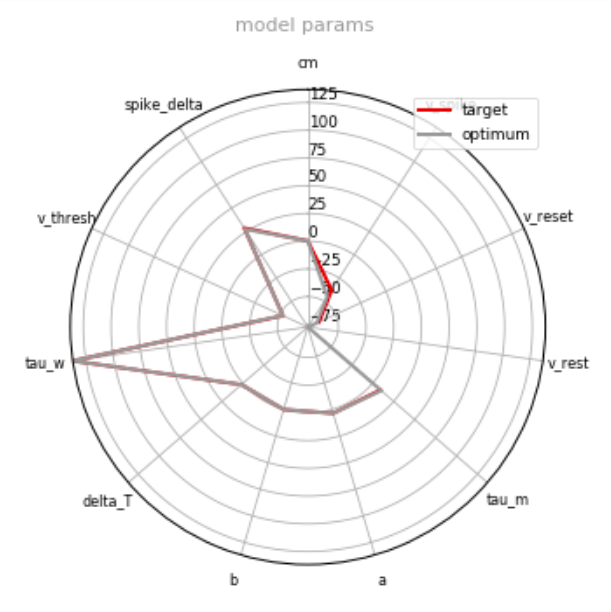
\includegraphics{figures/radar_coordinates.png}
    \caption{This radar plot of model parameters, reveals two mutually inclusive sets, both model parameter values 1 randomly selected, 2 found by the optimizer closely match.}
    \label{fig:my_label}
\end{figure}


%coincide 


\begin{figure}
    \centering
    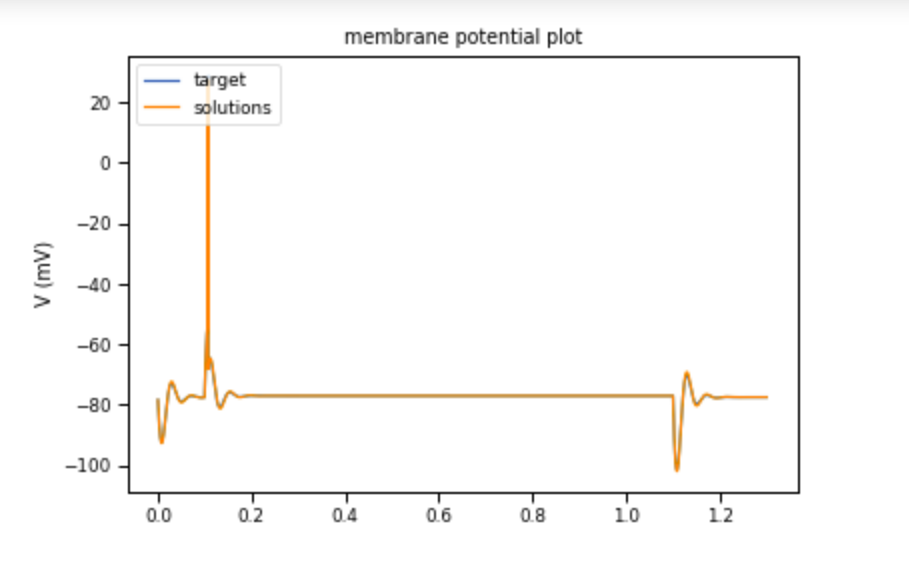
\includegraphics[scale=0.75]{figures/simulated_data_supra_threshold.png}
    \caption{Caption}
    \label{fig:my_label}
\end{figure}
\begin{figure}
    \centering
    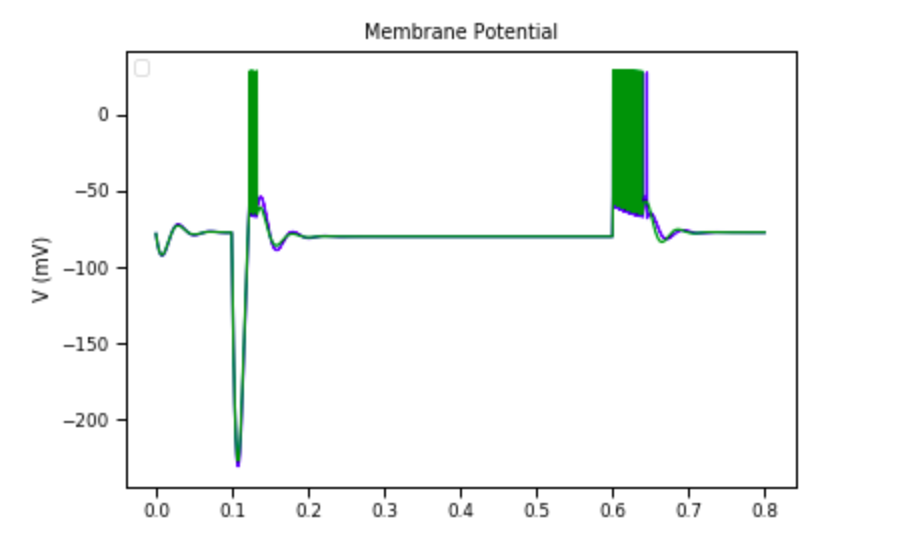
\includegraphics[scale=0.75]{figures/simulated_data_sub_threshold.png}
    \caption{Agreement between a simulated waveform, and an optimized waveform, when both simulated constraint model and optimized model undergo a current injection value of $-10pA$}
    \label{fig:adexp_model_rebound_spike}
\end{figure}

\begin{figure}
    \begin{center}
    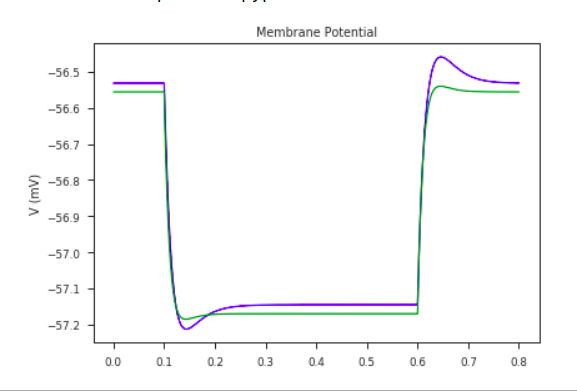
\includegraphics[scale=0.65]{figures/passive_model_agreement}
    \caption{For contrast, this is the Izhikevich model undergoing the same $-10.pA$ current injection value. There is no rebound spike. The model with the blue trace does rebound slightly. Agreement between a simulated constraint waveform, and an optimized waveform, when both simulated constraint model and optimized model undergo a current injection value of $-10pA$}
    \end{center}
    \label{fig:my_label}
\end{figure}

The plot of model membrane potential, as the model undergo's a $-10pA$ current injection, contains multiple spikes in the presence of an inhibitory current is unexpected. The reason this occurs, is because of an unusual model parameterization that makes modelled neuron "rebound spike" in response to attempts to move membrane potential down with voltage.



\ref{fig:adexp_model_rebound_spike}

\begin{comment}

\begin{figure}
    \centering
  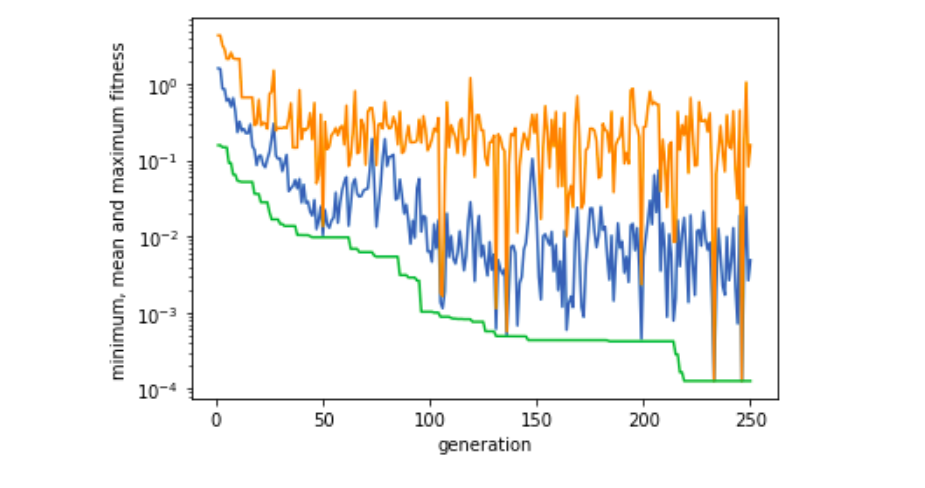
\includegraphics{figures/simulated_data_stats.png}
    \caption{Optimizer evolution, green line tracks evolution of best fitness, blue line average fitness, orange line is worst fitness. GA params, $NGEN=200$, $MU=50$,$cxp=0.3$,$mupb=0.2$ from this plot can see that genes are storing and exploiting information, $cxp+mutpb=0.5$, so $50\%$ of genes are conserved between generations }
    \label{fig:my_label}
\end{figure}
\end{comment}

\begin{figure}
    \centering
    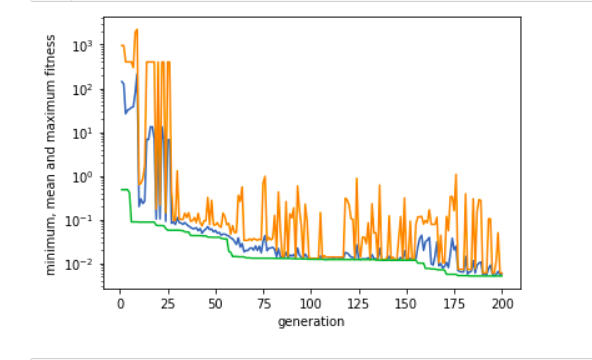
\includegraphics[scale=0.7]{figures/optimizer_internal_validation}
    \caption[Optimizer error over generations]{Optimizer evolution, green line tracks evolution of best fitness, blue line average fitness, orange line is worst fitness. GA params, $NGEN=200$, $MU=50$,$cxp=0.3$,$mupb=0.2$ from this plot can see that genes are storing and exploiting information, $cxp+mutpb=0.5$, a changing number of genes are conserved between generations }
    \label{fig:my_label}
\end{figure}


\begin{table}[ht]
\centering
\resizebox{\textwidth}{!}{
\begin{tabular}{llll}
\toprule
{} &    observations &     predictions & Z-Scores \\
\midrule
RheobaseTest         &         1.62 pA &         1.62 pA &        0 \\
TimeConstantTest     &        13.18 ms &        13.18 ms &        0 \\
RestingPotentialTest &       -77.43 mV &       -77.43 mV &        0 \\
InputResistanceTest  &  270.84 megaohm &  270.84 megaohm &        0 \\
CapacitanceTest      &        48.65 pF &        48.65 pF &        0 \\
FITest               &    7.51 Hz/pA &    7.51 Hz/pA &        0 \\
\bottomrule
\end{tabular}}
\end{table}

AP width, amplitude, and AP threshold errors, did not participate in guiding optimization, because as I have explained, those measurements are not objective between model instances, and thus they lead to misleading error measurements. These tables show that the optimizer can recover ground truths that are derived from simulated data. This result allows us to confidently argue that in fitted models, the cause of model/experiment disagreement must be located in either the data, or the models, but not the optimization process, or the choice of error signals which are demonstrably sound.

%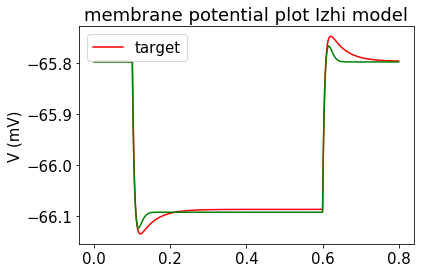
\includegraphics[]{figures/simulated_data_convergence_passive_fits.png}





% probably discussed elsewhere The design of the optimizer used in this work computed rheobase for each model, what that means is a new value of current is required to apply current injection tests to tests that are spiking in nature.\\
%In the optimizer design used here.

%$N-free-model-parameters << N-constraints$
%$(model parameters + %current-injection-value-parameter) << N$ $(independent and uncorrelated)$ constraints.

For the different classes of Reduced Model we show that the optimizer converges when data is simulated.

In a simulated experiment, existing models were instantiated using a randomly chosen model parameters.

The AdExp model, is not an arbitrary waveform generators. Models such as AdExp have intrinsic restrictions that prevent them from matching perfectly with all types of experimental waveforms.


%In the class of reduced neural models we optimized 

When constraints are derived from model measurements, intrinsic model restrictions no longer apply. Optimized models should match perfectly with the simulated experiments. 

* Failure to match is indicative of: -- Failure to setup tractable optimization problems, and under constraining  a high dimensional problem.

- When inverting linear equations, finding a unique solution requires that the number of constraining equations is greater than the number of free variables you are solving for. Analogous to a mathematical technique: Gaussian elimination where unknown variables are solved for using inversion and elimination, in genetic algorithm we solve for unknown variables using stochastic principles, however, underneath implementation details a similar principal exists: Larger amounts of known information can be used to solve for smaller amounts of unknown information. In other words assuming that NOBJ consist of only informative convex error surfaces as a rule of thumb optimization will likely be easy if $NDIM<NOBJ$.

\subsection{Pitfalls}
Choosing optimizer constraints, that cause visible ripples in error surface.
To protect against a situation where the collection of error sources guiding optimization are too correlated with each other, to act as 


\subsection{Verification}
Ground truths are model solutions that we know are correct independently from the optimizer. One way to establish ground truths is to identify the global minima by exhaustively searching the solution space. An exhaustive search is a reasonable approach when you consider only one or two model parameters are free parameters, however if one does 100 samples in each of N dimensions then one must make samples $100^{N}$ total samples to be sure of ehaustively searching, assuming the most efficient code, hardware and development time $N=3$, may be the highs.  Also the choice of 100 samples is nominal, 100 samples could be either too fine or too sparse, depending on how if the parameter being searched exhibits 2nd order sensitivity.

It is more computationally efficient to obtain ground truths by simulating constraining data using digital models. It is easy to simulate constraining data, all that is required is that you take a neuronal model and measure its behavior in response to carefuly chosen current injection values. Measured behavior can then be used to construct NeuronUnit tests, were the measurements become "observations", or observed behaviors. To make the simulated data cover a range of circumstances, one can make different NU measurements by randomly choosing different parameter values of models to find.

It was important to be able to establish ground truths that were always possible for the optimizer to match exactly. Often experimental data implies waveform shapes that are beyond the capabilities of the model that is to be fitted. Simulating experimental measurements meant, that model limitations can be understood separately from optimizer limitations.

 % ie is optimizaation possible?

\section{Limitations of Optimization using Experimental Data}
\label{sec:limitations-of-optimization}

\subsection{When is Optimization Possible Using Real Biological Data?}
Not all of the available data-sets are conducive to optimizing reduced models.
For example, consider the cerebellar Purkinje cell.
The Purkinje cells has a very large surface area (much of it the dendrites that support $~100,000$ synaptic inputs).
It consequently has a large capacitance and a low input resistance, and as such it demands a very large current stimulus to elicit a rheobase spike: $680pA$.
However, most reduced cells typically cannot exhibit such a large rheobase under any parameterization that otherwise looks like a neuron model.
The fact that an expansive dendritic tree is able to absorb so much somatically injected current may be difficult for a reduced model to capture.
Specifically, the upper limit for rheobase found in results was typically as $350-400pA$, but even this comes at the expense of sacrificing fit quality for all other electrophysiological features.
Consequently, optimized models of the Purkinje cell always failed to be biologically plausible.
The p-value of the $\chi^{2}$ statistic was always sufficiently low to reject the null hypothesis that such optimized models were representative of the biological data distribution.
Like the Purkinje cell, the Mitral cells of the main olfactory bulb also escaped successful model fitting.
These mitral cells also have high membrane capacitance $235pF$, and reduced models could not reproduce their features well.  
The Izhikevich model was achieved the lowest overall $\chi^{2}$ statistic for Purkinje cells and Mitral cells, being slightly more flexible than the AdEx or  conductance based models (see Tables \ref{tab:adex-allen} and \ref{tab:izhikevich-allen}).
In general, however, these reduced models may have been developed with smaller, more electronically compact cortical and hippocampal cells in mind.

\subsection{Conflicts between Experimental Features Constraining Optimization}
Feature values extracted from multiple data sets appeared to be in conflict for some cell types.
For example in the section below I show that the rheobase value was often incompatible with some passive electrophysiological feature values, such that good optimization could be achieved with one set or the other, but not both together.

\subsubsection{Tradeoff Patterns in Data-driven Tests in Subtheshold and at Threshold Electrical Properties}
\label{sec:rh_incomp}
Using data from the Allen Cell Types neuron with ID $471819401$,
I was able to optimize both AdEx and Izhkevich models, such that both models would agree with rheobase, time constant, resting membrane potential, and input resistance, experimental values. Some tradeoffs were needed in order match all of the values, as these features could not all be perfectly matched at once.
\begin{table}
\begin{center}
\begin{tabular}{|l|l|l|l|}
\toprule
Test name &   observations &    predictions & Z-Scores \\
\midrule
RheobaseTest         &       190.0 pA &      199.52 pA &     0.04 \\
TimeConstantTest     &        13.8 ms &        6.21 ms &     0.32 \\
RestingPotentialTest &       -77.5 mV &      -39.29 mV &     0.26 \\
InputResistanceTest  &  132.0 megaohm &  44.94 megaohm &     0.45 \\
\bottomrule
\end{tabular}
\caption[AdEx model fit quality]{Predicted and observed features for neuron $471819401$ from the Allen Cell Types database, following optimization of the AdEx model against data from this neuron.
Other neurons showed similar optimization performance, and are shown in the Appendix.}
\label{tab:adex-allen}
\end{center}
\end{table}

\begin{table}
\begin{center}
\begin{tabular}{|l|l|l|l|}
\toprule
{} &   observations &    predictions & Z-Scores \\
\midrule
RheobaseTest         &       190.0 pA &      190.48 pA &        0 \\
TimeConstantTest     &        13.8 ms &         1.9 ms &     0.94 \\
RestingPotentialTest &       -77.5 mV &      -70.65 mV &     0.03 \\
InputResistanceTest  &  132.0 $M\Omega$ &  25.47 $M\Omega$ &     0.74 \\
\bottomrule
\end{tabular}
\caption[AdEx model fit quality]{Same as the Table \ref{tab:adex-allen} but for the Izhikevich model.}
\label{tab:izhikevich-allen}
\end{center}
\end{table}

%And different specimen id's For example: 482493761 id:
%Adex:
%\newline
%\begin{center}
%\begin{tabular}{|l|l|l|l|}
%\toprule
%Feature Name &   observations &               predictions & Z-Scores \\
%\midrule
%RheobaseTest         &        70.0 pA &                   73.4 pA &     0.04 \\
%TimeConstantTest     &        24.4 ms &  0.0029 ms &     9.32 \\
%RestingPotentialTest &       -71.6 mV &                 -49.76 mV &     0.13 \\
%InputResistanceTest  &  132.0 megaohm &             72.15 megaohm &     0.23 \\
%\bottomrule
%\end{tabular}
%\end{center}
%\end{table}


%Izhikevich:
%\begin{table}
%\begin{center}
%\begin{tabular}{|l|l|l|l|}
%\toprule
%{} &   observations &    predictions & Z-Scores \\
%\midrule
%RheobaseTest         &        70.0 pA &       71.19 pA &     0.01 \\
%TimeConstantTest     &        24.4 ms &        2.85 ms &     1.05 \\
%RestingPotentialTest &       -71.6 mV &      -55.05 mV &      0.1 \\
%InputResistanceTest  &  132.0 megaohm &  46.06 $M\Ohm$ &     0.43 \\
%\bottomrule
%\end{tabular}
%\end{center}
%\end{table}


%\begin{table}
\subsubsection{6239608801 AdEx}
The need to match the rheobase appeared to be interfering with the ability of the optimizers to match many other features.
The rheobase is essentially the knee of the FI curve.
An alternative strategy is to produce models that match the slope of the FI curve.
Here I show two out of $12$ examples demonstrating that that fitting models to the FISlope and rheobase only, leads to generally better agreement as there is less conflict between these two tests.
%\textbf{Model Parameters}
%\newline
%\begin{center}
%\resizebox{0.7\textwidth}{!}{
%\begin{tabular}{|l|r|r|r|r|r|r|r|r|r|r|r|}
%\toprule
%{} &          cm &    v\_spike &    v\_reset &     %v\_rest &      tau\_m &         a &         b &   delta\_T &       tau\_w &   v\_thresh &  spike\_delta \\
%\midrule
%0 &  147.166079 & -45.027618 & -32.175811 & -51.521467 &  51.323969 &  1.787643 &  5.553571 &  4.143261 &  158.661633 & -25.749411 &    15.471554 \\
%\bottomrule
%\end{tabular}}
%\newline
%\end{center}
%\end{table}

\begin{table}
\begin{center}
\begin{tabular}{|l|l|l|l|}
\toprule
{} & observations &   predictions & Z-Scores \\
\midrule
FITest       &   0.18 Hz/pA &  0.18 Hz/pA &     0.01 \\
RheobaseTest &      70.0 pA &      70.26 pA &        0 \\
\bottomrule
\end{tabular}
\end{center}
\end{table}

\begin{table}
\begin{center}
\begin{tabular}{|l|r|}
\toprule
chi\_square &  0.000083 \\
p\_value    &  1.000000 \\
\bottomrule
\end{tabular}
\end{center}
\caption[Quality of Fit to Experimental Data]{Summary statistics of fit quality using AdEx model, when it is constrained against FITest, and Rheobase Test alone.
The very low $\chi^2$ statistic (and high p-value) indicate that there was no evidence that this optimized cell model produced behavior outside of the range of biological neurons of the same type, at least for the features examined here.}
\label{tab:chi2-p-1}
\end{table}

%\newline

\subsubsection{6239608801 Izhikevich}

%\newline
%\textbf{Model Parameters}
%\newline
%\begin{center}

%\begin{tabular}{|l|r|r|r|r|r|r|r|r|r|r|}
%\toprule
%{} &           C &        k &         vr &         vt &      vPeak &        a &          b &          c &          d &  celltype \\
%\midrule
%0 &  190.848367 &  0.77007 & -65.461028 & -49.496538 &  31.461532 &  0.05877 &  13.916167 & -58.159122 &  38.738638 &         7 \\
%\bottomrule
%\end{tabular}}
%\end{center}


\begin{table}
\begin{center}
\begin{tabular}{|l|l|l|l|}
\toprule
Features & observations &   predictions & Z-Scores \\
\midrule
FITest       &   0.18 Hz/pA &  0.18 Hz/pA &        0 \\
RheobaseTest &      70.0 pA &      66.61 pA &     0.04 \\
\bottomrule
\end{tabular}
\end{center}
\begin{center}
\begin{tabular}{|l|r|}
\toprule
chi\_square &  0.00155 \\
p\_value    &  1.00000 \\
\bottomrule
\end{tabular}
\caption[Quality of Fit to Experimental Data]{Similar to Table \ref{tab:chi2-p-1}, but for Izhikevich model. Since two major model classes are better able to fit to FITest and Rheobase alone, it suggests that these two measurements might be less conflicted in models.
}
\end{center}
\end{table}


By ``good optimization" I mean that the optimized model exhibited behavior that was consistent with all of the features.
Models seemed to have particular difficulty in recapitulating an accurate fit for rheobase, while simultaneously satisfying the fitness criteria imposed by the time constant, input resistance, capacitance and resting membrane potential.
This was less problematic when using the slope of the FI curve as a feature, suggested that it was not spiking \emph{per se} that caused the problem.

This was also evident when working across datasets.
For example, when optimizing against data from both NeuroElectro and the Allen Cell types database, it was typically impossible to satisfy data-derived features from both sources simultaneously, even when the same nominal neuron type was being described.

%The l5pc model was pre-optimized to fit to spike times and F/I mainly, and so it should not necessarily be expected to fit other electrical characteristics of the cell. Only the rheobase test, and the time constant test seemed to fall within the range of biological plausibility. None the less, this model remains a useful benchmark for reduced neuronal models.
%It was desirable to include this extended range of Izhikevich model behavior
%However, as noted in the introductory material, it i 
%Previously I mentioned neuronal modelling competitions I have optimize every model against the same data sets in order to assess overall which model is better able to fit to diverse data sets.

%
%\begin{comment}
%\subsection{Neocortical Layer 4/5 Pyramidal Cell Test Suite}
%\subsection{%2a}
%Direct Quote: "widening of the spike shape, decrease of the firing rate and change in the interspike interval distribution". %All these single unit waveform shapes increased their width with temperature.\cite{goldin2017temperature}

%1a/b Is Optimization possible?
%       1a. Construction of tests from diverse experimental sources (I wrote the neuroelectro api and its use in neuronunit, and wrote the original Allen one, but you have put in work to create runnable tests from these and other sources).  This is in a sense a method, but you can still report that these tests are runnable, even outside of optimization.
%       1b. Simulated data tests of optimization.  What works?  What doesn’t?  Why (briefly, saving some for discussion)?  NeuroElectro vs Allen also belong here, and fits in with 1a.  You should talk about model means vs means of models (or whatever we are calling it) here, if you have the results for it or think you can in 3 weeks.  
       %You can talk about rippled error surfaces — this is such a deep technical detail that I wouldn’t spend a lot of time on it.  In other words it may be important but it will be almost impossible to follow even if written well.


%During optimization knowledge of error surfaces should not be mandatory but it can help to solidify good optimization outcomes.  Through human examination of resulting error surfaces, it was found that some of the novel test sets were not helpful to the optimization framework.  Interestingly some types of tests had a propensity to amplify errors originating from elsewhere.

% depended on current stimulus values that were not fixed between models, but instead where contingent on the changeable state of the model cell, this measurement was usually the derivative of membrane potential: $max(\frac{dV_{m}}{dt})/10$. For more on this see \ref{sec:Optimization Pitfalls} 
% duplication
%I found that some fraction of these new tests were because they depended on measured features relative to some other changeable measurement inside the cell usually $max(\frac{dV_{m}}{dt})/10.$ As I discuss in methods, had the propensity of amplifying errors that propogated from elsewhere. 
%This required both the extraction of novel features [EFEL: ISI, AHP-depth, adaption ratio etc.] on new data types types.

%This class was also acculated useful helpful methods such as retrieving default model parameters.



%Flat regions of error surface are uninformative.
Tests that the author curated from Allen Cell types led to some models being under-constrained about spike width. The severe consequences of under-restraining were not obvious, they were revealed by graphs in a virtual experiments were appropriate models were elicited to spike. The lack of constraint was easily rectified, by imposing a specific spike width constraint on Adaptive exponential models, however, unexpectedly in this context, the models $\chi^{2}$ increased dramatically and biological plausibility plummeted, in all except one test. To  paraphrase, the adaptive exponential models had found an unexpected way to cheat tests, by taking advantage of a lack of constraints in an unrelated area.



There was a need to create extra constraints for fitting models, as the set of Allen Constraints was too few in extent, and not sufficient to properly constrain models.



In type of standard, the NeuronUnit tests, themselves act as the final judge of model quality, in the absence of a spike width tests, many AdExp models were able to get very good fits on against supplied constraints, but plots of actual spike shape looked very unnatural, as spike width lasted $>=$ 6ms. Applying extra standards beyond the NeuronUnit tests creates a dilemna. As all the GLIF models, presented unusual spike shapes.


\subsubsection{Experiment Fitted Model Results} 

%Allen Brain Institute, Cell-types E-Physiological data, Elephant Tests
%\subsection{Experiment Fitted Results Neuroelectro data, Elephant Tests}

Over four different Allen experimental sweeps, and four different different cell type specific electrical observations, we created eight unique data sets, and then converted these eight data sets to neuronunit test suites.

We then took four different models, and we attempted to fit each test set to each model. The result of was a four $\times $ eight factorial of model data combinations. For each each member of this 32 set factorial we wanted to know if the fitted model behaved in a biological plausible manner, we were interested to know if fitted models were convincing mimics of in-vivo cells, at least with respect to the measurements models were trained to fit.


\subsection{Standard Error of the Mean}
\begin{tabular}{lrrrrrrr}
\toprule
{} &  Rheobase &  SpikeThreshold &  SpikeHalfWidth &  SpikeAmplitude &  MembraneTimeConstant &  RestingMembranePotential &  InputResistance \\
sem                                &           &                 &                 &                 &                       &                           &                  \\
\midrule
Hippocampus CA1 pyramidal cell     &    122.88 &            1.85 &            0.12 &            3.68 &                  3.88 &                      0.72 &            12.57 \\
Olfactory bulb (main) mitral cell  &       NaN &            5.69 &            0.12 &            2.83 &                  5.42 &                      1.39 &            20.17 \\
Cerebellum Purkinje cell           &    419.81 &            2.00 &            0.05 &            0.57 &                   NaN &                      3.69 &            19.26 \\
Neocortex pyramidal cell layer 5-6 &    128.87 &            1.92 &            0.17 &            1.49 &                  2.56 &                      1.84 &            27.93 \\
\bottomrule
\end{tabular}


Since some of the NeuroElectro data sources were more challenging to fit, we also computed the Standard Error of the Mean, so that later we could interprite model fitting failure. Forinstance, the SEM is a prediction of a measurements dispersal, it is often used when the standard deviation is unknown. 

The $\chi^{2}$ statistic, and the p-value give us a formally indicates how convincing each fitted model was in its mimicry of biological measurements.
Because we already have a list of Z-scores, the $\chi^{2} $statistic can be obtained by squaring each Z-score and summing the result. A sum of squares less than 1, tells us that models performed well.
$\chi^{2}=\Sigma_{i} (Zscore_{i}^{2}) $

%https://en.wikipedia.org/wiki/Chi-square_distribution
%This allows you to state this as a hypothesis test with a p-value.  The chi-square statistic would simply be , and the p-value would be 1-scipy.stats.chi2.cdf(x, 8) where 8 is the number of elephant tests (and Z-scores).  A very small p-value (which would come from very large chi-square statistic, much larger than expected for random variation) %would mean the optimizer was less successful at recovering the true model.

See appendix:\ref{table:static_electrical_properties}
The Izhikevich Model and the Point Conductance Model were able to achieve high p-values, and small chi-squared statistics when seven or eight of the tests were considered together.

For example the Izhikevich model fitted to Hippocampus CA1 pyramidal cell data achieved $ (\chi^{2} ,p-value) =(2.1250913868824415, 0.9769347643323284) $

The olfactory Mitral cell
$ (\chi^{2} ,p-value) =(2.0190436240810925, 0.9804224622781068) $

and the cerebellum Purkinje cell. For contrast p-value and chi-squared statistics on the best random models were:

%(2.0190436240810925, 0.9804224622781068)r
\subsection{Data fitted Results on four different classes of model were only modestly good for the Izhikevich Model and the Point Conductance Model}

To make the argument that limitations in reduced neural models were the cause of modest model/experiment agreement, we first had to rule out alternative possibilities. One possibility was that the experimental measurements were faulty, and that the measurements were possibly spurious because of in appropriate averaging. It was found that mainly the olfactory bulb mitral cell was prone to having underlying bi-modal data distributions, and this was especially true for resting membrane

that the models shouldn't be able to reproduce. When considering the data sources, the methods of data collection and data quality should be reliable, the one main 

we first needed to exclude the possibility that there might be something wrong with the data, we are fitting models to.

We needed to rule out was that the data sources did not reflect bi-modal distributions, since the neuroelectro data was the actually the mean over different laboratories, animals, and recording epochs. The mean of a population can often be a robust representation of a population, however there are circumstances when the opposite is true, such as when the underlying data is generated by two different processes, leading to bimodal distributions. Fortunately, it is not hard to test if experimental data, has an underlying bimodal distribution. That test was performed using human judgement for all measurements that were used to fit the model to experiments. Except in the case of the Allen Brain data, because the Allen Brain data consisted of individual raw experiments, and population averaging did not apply. For measurements used in the elephant optimization pipeline.

Below I show distributions for  Time Constant, Input Resistance, Capacitance, Rheobase, Resting Membrane Potential, bimodal distributions did not apply, so we could rule out inaccurate data as a reason for poor model performance.

There is no reason to believe that reduced neural models could not be made to fit inaccurate neural recordings as well as real ones, if the fiction is just caused by noise, then it is still possible that hypothetical spurious values would still be in reach of the Izhikevich model. The izhikevich model can be made to generate some physiologically implausible waveform shapes. 
% a different question, of are the models arbitary waveform generators? 

Besides even if the data was wrong, it wouldn't necessarily follow that models couldn't reproduce the inaccurate data. Instead what we see is, that models can fit one type of experimental measurement at a time, but they can't fit all measurements at once. This result suggests that model flexibility is the most fundamental cause of modest, model experiment disagreement.


%In light of this result, one might ask, i
If reduced models are not excellent at fitting data, are brain simulations really that much more realistic, when we use data driven fitted models in the place of generic model parameters? If data driven model fits lead to models that fit one measurement better than others, which fitness criteria will lead to the greatest consequence for network simulations?

%to answer that question we have created some large




\section{Limitations data we were using was of Existing Approaches} 
Existing community supported simulated models were problem ridden, and our own custom methods were used as work arounds.

% NEURON version of Izhi model is not as fast as one might expect, this may because of the way we tried to implement the model, by creating and destroying HOC module instances, that contain the model. 

%A
% Nonetheless, 
At first we accessed an implementation of the Izhikevich model that was translated from jNEUROML into a NEURON simulator implementation. The problem with this implementation is that it had fragmented the whole Izhikevich model into chattering and non chattering subtypes. The model implementation seemed to have an internal conflict between two capacitive terms. The problem was that the Izhikevich model requires only one capacitive term.

implemented in NEURON which was derived from a J-NeuroML translation, could not reproduce all of the Izhi original publication figures, because it had two different conflicting sources of capacitance.\\
\\
From J-NeuroML we created NEURON version of Izhikich model, however we were not able to make this model execution times brief enough to be useful for optimization. Although the NEURON simulator is designed to be fast, their may be a cost associated with reloading the NEURON environment many times in fast succession.

This should not go in the general introduction, but in the intro to the appropriate section of the results where you use those models. 
\subsection{Does an Averaged Model Recapitulate Averaged Measurements?}
For a selection of three model measurements:

We are interested in the question: ``Could misrepresented data, lead to a situation were models try too hard to match targets that the models were not built to explain?" %We were interested in the consequence of this worst case. 

I placed two different versions of the same  model class in different locations of parameter space. For each location I measured: rheobase, input resistance, capacitance, and membrane time constant.
I then averaged these measurements together to obtain a mean set of electrical measurements, its this collection of measurements that I refer to as "mean measurements". Next we created a "mean model' by averaging the locations in parameter space together.
In averaging between two points we create a third point that is midway between the pre-existing coordinates. I refer to the third midway point as a "mean-model".
The mean model is used to create a third set of model measurements, as we are really interested in the question: "Does the mean model sometimes fail to recapitulate the mean measurement?"


%With these different parameter sets we took separate measurements of the listed electrical properties, 
When we have mean measurements, and also mean model measurements, it enables us to understand if bi-modal distributions of measurements in experimental data can pose a problem for optimization of cells.

Previously in methods \ref{section:nelectro}, we graphically inspected the neuroelectro data sources closely, in order to assess each measurements distribution.
We revealed Bi-modal distributions in input resistance, and cell membrane capacitance, but we do not yet know if it is invalid to fit to the mean of a bi-modal distribution.
Consider a  cell class which had an underlying bimodal distribution for input resistance. An individual cell from this class produced measurements for input resistance midway between two modes for input resistance.
Its entirely conceivable that that this mean cell would produce measurements that were also the mean of the two modes, however, we cannot assume that there this to be true, it seems equally likely that this midway cell produces a measurement for input resistance, that is significantly higher or lower than the mean of the two modes. To bolster that this non linear behavior could be a problem with in-silico models of in-vivo experiments.
We created virtual experiments to expose non-linear behavior between two  close, but different sets of model parameters.

%set about establishing that it is a problem in modelling space.
%The genetic algorithm approach, of recombining model parameters to sample error surface is a similar concept. We do not naively interpolate using midway points, becuase we don't expect that small changes in model parameters to have linear effects.
%to sampling models 

We expect the Izhikevich model, and the adaptive exponential models to support ``regime" change, that is we know that there are regions in parameter space that where when entered cell behavior becomes fundamentally different. For instance in the Izhikevich model, some regions support tonic-bursting and other regions support chattering. 

\begin{figure}
    \centering
    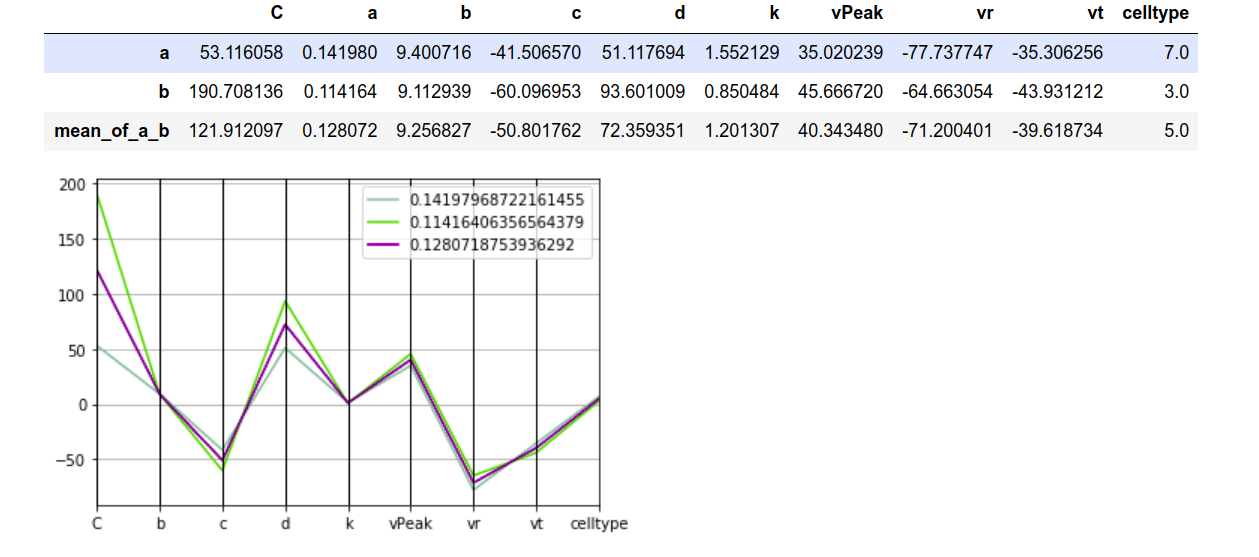
\includegraphics{figures/mean_model_mean_measure_ment_params.png}
    \caption{Caption}
    \label{fig:my_label}
\end{figure}

\begin{figure}
    \centering
    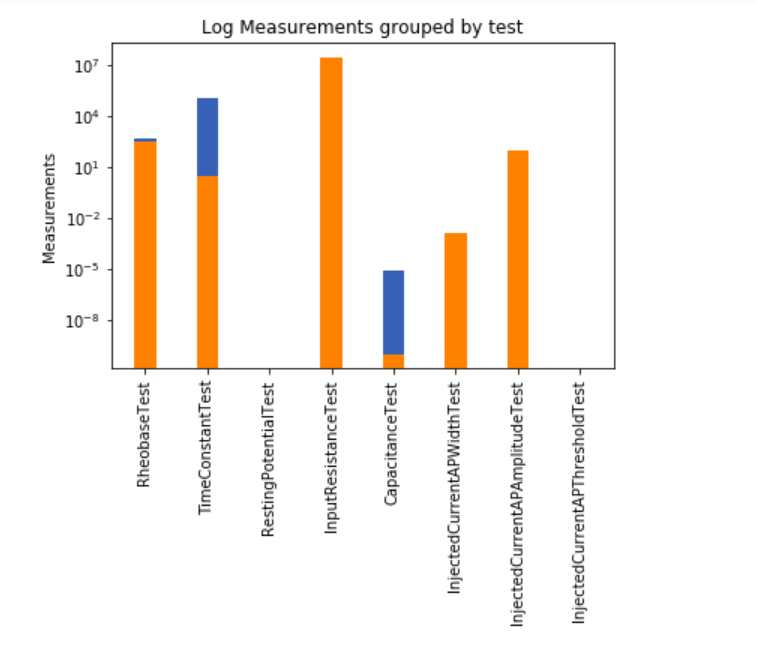
\includegraphics{figures/mean_model_mean_test.png}
    \caption{Caption}
    \label{fig:my_label}
\end{figure}

\begin{figure}
    \centering
    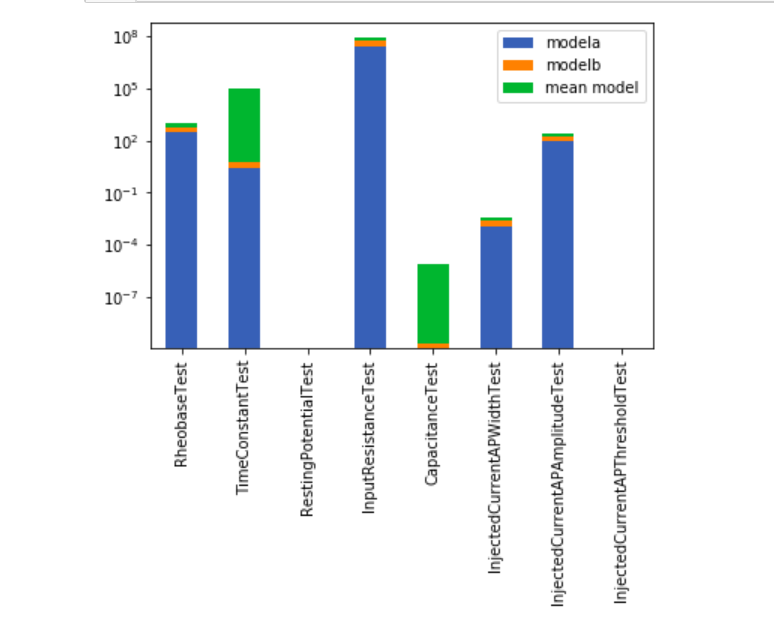
\includegraphics{figures/mean_model_mean_test2.png}
    \caption{Caption}
    \label{fig:my_label}
\end{figure}

explore if this was a problem for models as well as experimental cells.
%Previously, the INCF hosted a model data fitting competition, were participants competed to submit models that %were best able to fit membrane voltage from a variety of above-threshold current injection experiments see %figure \ref{fig:}. In this competition, unlike in this work the best models had to predict spike time. Within %the scope of this project, post-optimization, ranking of the different models in terms of their ability to %explain the most in-vivo experiments.  There are some data sources, that no models seem to do well on, however, %the majority of experiments cause good fits, and the models should compete with each other.
%\subsection{Neocortical Layer 4/5 Pyramidal Cell Test Suite}

%Direct Quote: "widening of the spike shape, decrease of the firing rate and change in the interspike interval distribution". %All these single unit waveform shapes increased their width with temperature.\cite{goldin2017temperature}



%\subsubsection{%\subsection{Section 2.1}
%
%2. Results for several optimized models.
%    2a. First just do basic ones (like Izhikevich) for a few cell types, then you can close with L5PC.
%    2b. The app (which supports 2a).

%\subsubsection{2a}

\section{Performance of Optimized Models}


\subsection{Somatosensory Layer 5 Pyramidal Neuron Model Applied to NeuronUnit Data Driven Tests}

Below I introduce a different approach to parameter fitting work: a multi-compartment, conductance based layer 5 pyramidal cell model \citep{van2016bluepyopt}, was appropriated from BluePyOpt optimization framework, and massaged into the NeuronUnit framework.
This model subserved as one of many component neurons in the original formulation of the Blue Brain Project \cite{markram2015reconstruction}.


This elaborate biophysical model is the philosophical opposite of the reduced models focused on in the majority of this thesis work, since the model incorporates electrically complex phenomena instead of excluding it from the model.
The complex model includes a dendritic action potential which can travel ``backwards" from distal dendrite to soma where it is free to summate with incoming EPSPs.
As you can see in the list of parameters (Figure \ref{fig:ca1_parameters}), The model has different adjustable conductance's in 3 out of 4 membrane domains including axons, dendrites, and soma. In the figure \ref{fig:brief_shape} you can membrane zones with different channels are color coded: apical dendrites (magenta), basal dendrites, and axons.


\begin{figure}%{.2\textwidth}
  \begin{center}
    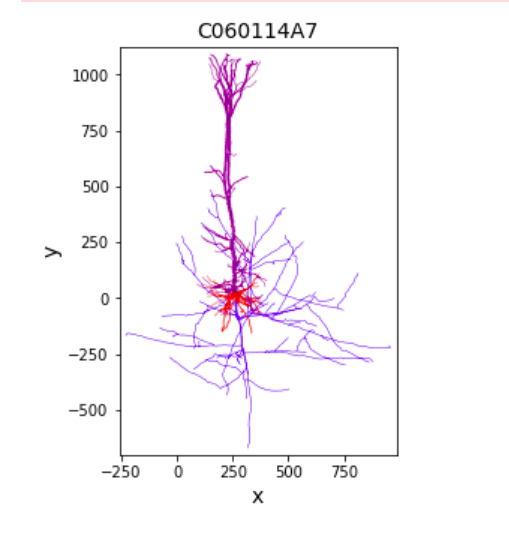
\includegraphics[scale=0.8]{figures/morphology_view.png}
    \caption[l5 pyramidal neuron tree]{This l5 pyramidal neuron model is spatially extended, so a 2D depiction of its dendrite and axonal tree is warranted.}
  \label{fig:brief_shape}
  \end{center}
\end{figure}


There are also other parameters (not displayed here) which are fixed, but those specified in Figure  \ref{fig:ca1_parameters} are amenable to fitting in the context of optimization.


An existing cell from the layer 5 somato sensory rat, hind leg region was acquired by cloning an the BluePyOpt GitHub Repository \cite{van2016bluepyopt}.
Neuroelectro lumps together, prefrontal cortex, somatosensory cortex and V1 PC cells together into a generic frontal cortex pyramidal cell model. 

% Overall it seems

%on NeuronUnit tests of model data agreement}
%\subsection{Section 2.1}
%
%, so it is probably not comparable to NeuroElectro Data.
A suite of neuronunit tests containing the tests: rheobase value, membrane voltage time constant ($Tau_{m}$), input resistance was computed. This multi-compartment, conductance based model served as a useful benchmark, for us to evaluate the relative performance of reduced model fits. 

%A test suite was constructed using NeuroElectro for the layer 4/5 Prefrontal Cortex pyramidal cell, and we were able to evaluate this layer 5 PC cells against the criteria of the neuroelectro test suite.


Significant development work went into making the model eligible to take NeuronUnit tests, by way of creating a specially dedicated NeuronUnit backend, to run this complicated conductance based multi-compartment model originating from the blue brain model \cite{markram2015reconstruction}. The intention is that by making this model interoperable with NeuronUnit the model will be able to amenable to optimization.


This elaborate biophysical model includes the backpropogating dendritic action potential.
\url{https://github.com/BlueBrain/BluePyOpt/blob/master/examples/l5pc/L5PC.ipynb}
\url{https://github.com/social-hacks-for-mental-health/BluePyOpt/blob/master/examples/l5pc/L5PC.ipynb}


It is possible that the majority neuroelectro recordings of L5PC, spike width were conducted under room temperature as opposed to body temperature, and the relative cooling may have contracted their spike width.
\cite{goldin2017temperature}

\begin{figure}
  \centering
    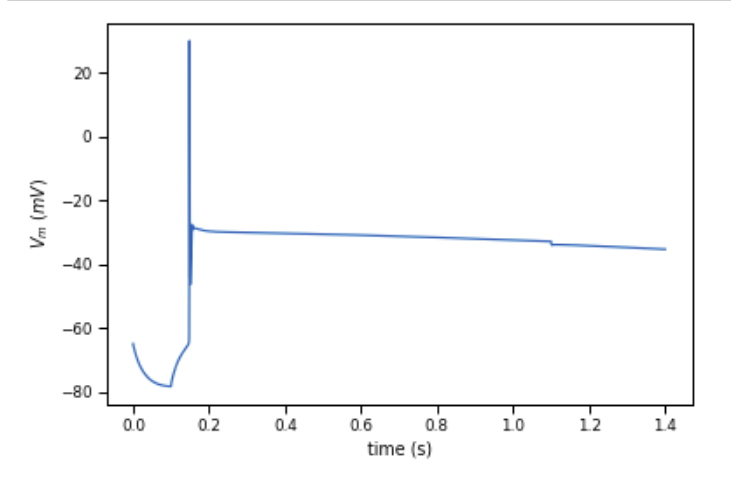
\includegraphics[scale=0.8]{figures/correct_active_l5pc.png}
    \caption[Short duration spike in the L5PC model]{A current injection sufficient for causing a single spike is applied to cell soma, for a whole second from $100ms-1100ms$ in this model. The spike shape is brief and more complicated than reduced model spike shapes. After the very brief spike soma voltage seems to plateau over the entire length of the simulation. The simulation is not long enough for the soma voltage to return to resting membrane potential}
  \label{fig:sub1}
\end{figure}

\begin{figure}
 \begin{center}
    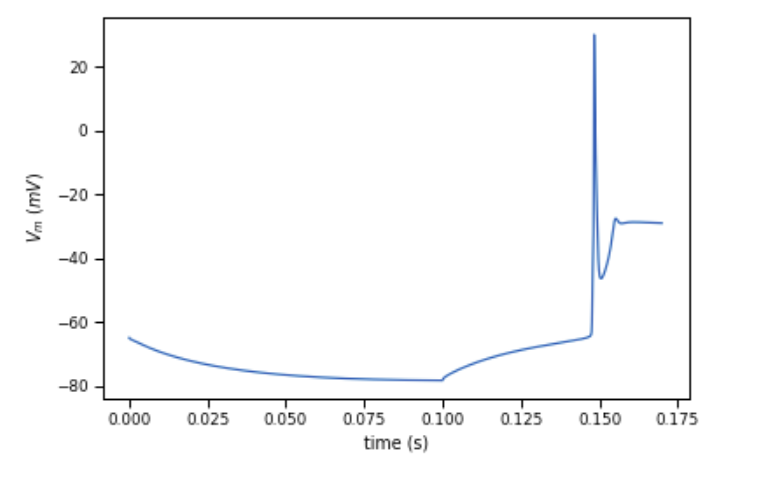
\includegraphics[scale=0.8]{figures/spike_shape.png}
    \caption[Complex spike in the L5PC model]{The above plot warranted a closer look, therefore, this plot features the same model and the same virtual experiment as above, only a smaller time interval has been inflated to fill the whole time axis. In this plot of increased time resolution there is a visible detour in the spikes path to re-polarisation. This unusual feature may be related to a back-propogating dendritic spike, which, a depolarisation wave may have returned from the distal dendrite and has re-invaded the soma, causing the voltage to plateau far above resting membrane potential. These are behaviors, that are obviously neglected in reduced model design}
  \label{fig:sub1}
  \end{center}
\end{figure}

\begin{figure}
\begin{center}
    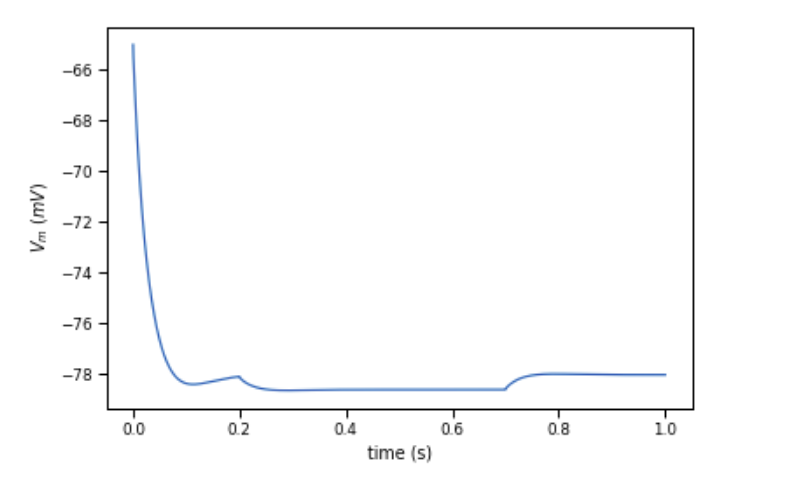
\includegraphics[scale=0.8]{figures/correct_passive_l5pc.png}
    \caption[passive virtual experiment in the Layer 5 Pyramidal Cell]{A current injection value of -$10pA$ is applied to the soma of the pyramidal cell for the duration of $200ms-700ms$. This plot shows the membrane potential at the soma of the multi-compartment model displaying overall expected behavior, the trough of the negative voltage deflection is not as deep as that seen in many reduced models. This suggests the small amplitude of the negative deflection suggests that the L5 PC model is has less resistance than most of the reduced models fitted to the same data, and indeed a low resistance measurement is confirmed in the table below.}
  \label{fig:sub2}
\end{center}
\end{figure}


\begin{table}[ht]
\centering
\resizebox{\textwidth}{!}{
\begin{tabular}{lllll}
\toprule
{} & observations &   predictions & Z-Scores & SEM \\
\midrule
RheobaseTest                   &    213.9 pA &      225.0 pA &  0.065 & 128.9 \\
InputResistanceTest            &  120.7 Mohm &  50.7 Mohm &  -0.90 & 27.9 \\
TimeConstantTest               &     15.7 ms &      16.76 ms &   0.14 & 2.6 \\
CapacitanceTest                &    150.6 pF &     330.7 pF &    1.28 & 1.49 \\
RestingPotentialTest           &    -68.3 mV &     -78.1 mV &   -1.5 & 44.0 \\
InjectedCurrentAPWidthTest     &      1.21 ms &       0.15 ms &   -1.98 & 0.175\\
InjectedCurrentAPAmplitudeTest &     80.4 mV &      89.6 mV &   0.72 & 1.49\\
InjectedCurrentAPThresholdTest &    -42.7 mV &     -59.6 mV &   -2.09 & 1.92\\
\bottomrule
\end{tabular}}
\caption[Z-scores, Observed and predicted features for The Layer 5 Pyramidal Cell]{As the Layer 5 pyramidal cell was made eligible for neuronunit testing. A suite of relevant Neuroelectro L5 Pyramidal cell tests were applied to this cell model iterative in an optimization framework. This table shows the end result of this process, where agreement between model and experiment has been maximized. The result of the test shows that the model falls within the range of biological plausibility, although model results are far from perfect in all tests. Notably the Rheobase value agrees well with experiments, as does the membrane time constant}
\end{table}


%\caption[Observed and Predicted L5PC]{Observations, predictions, and Z-scores pertaining to the NeuronUnit-optimized Layer 5 Pyramidal Neuron}
\label{tab:l5pc_table}
The corresponding statistics were
$(\chi^{2},p_{value})=(13.56, 0.094)$.
Note that the p-value is not sufficiently low to reject the null hypothesis that this model neuron is not from the same distribution as the biological/experimental results.
This may reflect the highly variable nature of the biological/experimental results, rather than the verisimilitude of the optimized model.
Nonetheless, given this experimental variability, the optimization is at least satisfactory. It is also worth noting that not all optimization results lead to the same solution, between different model fitting routines, the optimizer had to choose between fitting the membrane time, constant, fitting the spike width, and fitting the input resistance as the model could be made to fit only one of these measurements at a time. In other words in this model: input resistance, time constant, and spike width were conflicted.

%Hind-limb
%\cite{van2016bluepyopt}
%To understand the validity of model re-purposing, we tested a model constrained on Layer 5 Somatosensory cortex Pyramidal neurons. 

There were two points to this exercise: the first point was to show that multi-compartment conductance based models, are very slow to evaluate, and the second point was, that without enough time, the results are not necessarily as good as you would expect for the inclusion of additional complex mechanisms. There is an unintended straw man character to this observation, it's stipulated in the model documentation (a python notebook) that the model would require a run of at least $100$ generations and a population size of $100$ too properly optimize relative to a different set of constraints. Unfortunately I did not have the time or the computer resources to apply the specified optimization job. However these time considerations bolster a different assertion from my thesis work, timeliness of simulation results aids model refinement, whereby brief simulation times improves scientific insight.
However, the model itself happens to be a determining factor in reducing time. The resulting optimized model might serve as a useful benchmark, for us to evaluate the relative performance of reduced model fits. 

A suite of Neuronunit tests containing the tests: rheobase value, membrane voltage time constant ($\tau_{m}$), input resistance was computed. 
% somatosensory cortex, or cell from the l5 somatosensory rat, hind leg region, so it is probably not comparable to NeuroElectro Data.

Significant development work went into making the model eligible to take NeuronUnit tests, and amenable to NeuronUnit driven optimization, to make this complicated conductance based multi-compartment model interoperable with the NeuronUnit test judging paradigm.
The intention is that by making this model inter-operable with NeuronUnit the model will be able to amenable to different, optimization. 

%\begin{figure}
%    \begin{center}
%    \includegraphics{figures/l5pc_before_opt}
    % \label{fig:my_label}
%    \end{center}
%\end{figure}


%Behavior of the L5PC model is explored under three different stimulus strengths.

\begin{figure}
    \begin{center}
    \includegraphics{figures/l5pc}
    \caption[Behavior of the L5PC model under optimized parameters]{Behavior of the L5PC model is explored under only one stimulus strength. Membrane potential this time is viewed from recording locations in the soma and dendrites.  Membrane potential this time is viewed from recording locations in the soma and dendrites. In this recording site at the dendrite there is a singular backpropogating spike. Although the soma and axon hillock, trigger an adapting spike train, lasting more than a second, the dendrite only receives one backpropogating potential, which has a large spike half width. The reason the axon fires multiple times, but the dendrites fire once, is because  dendrites contain dominating passive mechanisms, that can low pass filter invading currents} 
    \label{fig:after_optimization}
    \end{center}
\end{figure}    
    %\caption[Behavior of the L5PC model before optimization under default parameters]{}
%   }


\begin{figure}
    \begin{center}
    \includegraphics{figures/parameters_opt_l5pc.png}
    \caption[Subset of modal parameters eligible for tuning in L5PC neuron]{Here I list not all the parameters of the layer 5 model, just the subset of adjustable parameters. The parameters that the genetic algorithm modifies, they are listed here with their default values. There are 20 different parameters that two different locations in the neuronal tree. The fact that there are 20 different dimensions to optimize over makes this problem especially intractible for the average researcher, since it is slow to evaluate as well as high dimensional. With the exception of the GLIF model, most models considered here are $<14$ parameters.}
    \label{fig:ca1_parameters}
    \end{center}
\end{figure}


%\begin{figure}
%\begin{center}
%   \includegraphics[scale=0.8]{figures/correct_a%ctive_l5pc.png}
%    \caption{A current injection sufficient for %causing a single spike is applied for a whole %second from $100ms-1100ms$}
%  \label{fig:sub1}
%  \end{center}
%\end{figure}

%As a reference point for understanding 
%    \caption{The spike shape is very brief in duration, and so it is worth zooming in for a closer look}

%\begin{figure}%{.2\textwidth}
%  \begin{center}
%    \includegraphics[scale=0.8]{figures/L5Somatosensory_not_optimized.png}
%    \caption[Plot of at threshold firing pyramidal neuron]{$V_{m}$ in $(mV)$ versus time $ms$, plots include a above threshold (top) and below threshold stimulus (below)}
%  \label{fig:brief_shape}
%  \end{center}
%\end{figure}

%\begin{figure}%{.2\textwidth}
%  \begin{center}
%    \includegraphics[scale=0.8]{figures/correct_passive_l5pc.png}
%    \caption[plot of negative amplitude current stimulus]{A current injection value of -$10pA$ is applied to the cell for the duration of $200ms-700ms$}
%  \label{fig:passive_properties}
%  \end{center}
%\end{figure}


A test suite was constructed using NeuroElectro for the non specific [cortical regions] layer 4/5 cortex pyramidal cell, and we were able to evaluate this layer 5 PC cells against the criteria of the neuroelectro test suite. Note the unnatural looking brief spike duration of the model cell spike  \ref{fig:brief_shape}. It is possible that the majority neuroelectro experiments on the layer 5 pyramidal cell were conducted under room temperature as opposed to body temperature, as there is evidence that the temperature of cortical tissue modulates spike width \cite{goldin2017temperature}, in particular cooling can contract their spike width

%%
% https://neuroelectro.org/data_table/36261/
%%
% from spike width table: 0.65 ± 0.13	1.04 ± 0.25**	0.51 ± 0.03**	0.59 ± 0.06	0.61 ± 0.03
%%
%


Due to computational limitations this model was only run for 
$12$ offspring, and $30$ generation. Actually a minimum of $\mu=100$, $NGEN =100$ was prescribed by the scientists who optimized the initial model, however such a large compute job required prohibitive computational resources.

The unoptimized model had statistics:
$(\chi^{2},p_{value})=(13.56, 0.094)$

The optimized model produced statistics
$(\chi^{2},p_{value})=(6.63, 0.57)$

Optimization then clearly improves the model, however, it does not bring the model  biological plausibity.
This can be improved by omitting some of the worst tests, overall, the tests are compromized.



It is worth noting that the layer 5 neocortical pyramidal neuron was very slow to dispatch relative to the reduced models developed in this thesis work. Where as a typical reduced model described here evaluated in the order of $~0.0025 seconds$, this model on average took $5.74$, for a single run and $34.8$ to solve for the models Rheobase, current.

This model was pre-optimized to fit to spike times and F/I mainly, and so it should not necassarily be expected to fit other electrical charactersistics of the cell. Only the rheobase test, and the time constant test seemed to fall within the range of biological plausibility.
None the less, this model remains a useful benchmark for reduced neuronal models. 
\subsection{Gallery of Model Fits to Supra-threshold Experiments}
\begin{comment}
\begin{figure}
    \centering
    \begin{subfigure}[t]
        \centering
        \includegraphics[width=0.5\linewidth]{example-image-a.pdf} 
        \caption{Generic} \label{fig:timing1}
    \end{subfigure}
    \hfill
    \begin{subfigure}[t]
        \centering
        \includegraphics[width=0.5\linewidth]{example-image-b.pdf} 
        \caption{Competitors} \label{fig:timing2}
    \end{subfigure}

    \vspace{1cm}
    \begin{subfigure}[t]
        \centering
        \includegraphics[width=0.5\linewidth]{example-image-c.pdf} 
        \caption{Price regulation} \label{fig:timing3}
    \end{subfigure}
    \hfill
    %\begin{subfigure}[t]%{0.45\textwidth}
    %    % just an empty subfigure to shift C below A
    %\end{subfigure}
    \caption{Some general caption of all the figures. In (\subref{fig:timing1}) you can see a  green square....}
\end{figure}
\end{comment}

% TODO make multi panel.

\begin{figure}
    \centering
    \includegraphics[scale=0.75]{figures/adexp_fit_allen_spec_id_476053392.png}
    \caption{An adaptive Exponential Model was fitted to both the spike time, and spike shape data in a sweep from Allen specimin id: 476053392} \label{fig:specimen_476053392}
\end{figure}

\begin{figure}
    \centering
    \includegraphics[scale=0.75]{figures/28spikesB95}
    \caption{An adaptive Exponential Model was fitted to both the spike time, and spike shape data in a sweep from Allen specimin id: 476053392} \label{fig:specimen_476053392}
\end{figure}

%Similar to Druckmann Suprathreshold depolarizing step currents \cite{druckmann2008evaluating}.
\begin{figure}
    \centering
    \includegraphics[scale=0.75]{figures/adexp_fit_allen_specid_325479788.png}
    \caption{ An adaptive Exponential Model was fitted to both the spike time, and spike shape data in a sweep from Allen specimin id: 325479788}
    \label{fig:specimen_325479788}
\end{figure}


% Interesting direct qoute from Druckmann:
%"In experiments, intrinsic noise gives rise to a large variability (e.g., in firing pattern) in the voltage responses to repetitions of the exact same input. Thus, the common approach of fitting models by attempting to perfectly replicate, point by point, a single chosen trace out of the spectrum of variable responses does not seem to do justice to the data."

%In experiments, however, when the exactly same stimulus is repeated several times, the voltage traces elicited differ among themselves to a significant degree (Mainen and Sejnowski, 1995; Nowak et al., 1997).

A joint collection of current injections and recordings known as sweeps were taken from a rat somato-sensory hind limb neuron.
\ref{fig:B95Adexp} is a challenging waveform to fit, as adaption does not predict the final ISI, which is smaller than the penultimate one. 

Although it is not obvious there is significant variation in ISIs (although the range of that variation may be concentrated within a small margin). As noted in the literature \cite{druckmann2007novel} it is probably mis-founded to over fit models to exact spike times because neurons themselves experience noisy intrinsic currents and they are likely to illicit different spike trains, given identical presentation of stimulus. In hind-sight I propose, to optimize on FI-slope and spike rate, while comprimizing on exact spike time agreement.

\begin{figure}
    \centering
    \includegraphics[scale=0.75]{figures/bbp_multispiking_fit.png}
    \caption{An adaptive Exponential Model was fitted to both the spike time, and spike shape data in a sweep from animal B95 
    %\url{http://microcircuits.epfl.ch/#/animal/8ecde7d1-b2d2-11e4-b949-6003088da632}
    Blue Brain Project. The base voltage. The base voltage, and Resting Membrane Potential, and spike numbers are matched, spike times are not perfectly aligned, spike height, and trough depth are not perfectly matched}
    \label{fig:B95Adexp}
\end{figure}

\begin{figure}
    \centering
    \includegraphics{figures/IZHI_B95.png}
    \caption{An Izhikevich model was fitted to both the spike time, and spike shape data in a sweep from Blue Brain Project. The Spike amplitude, and spike numbers are matched, spike times are not perfectly aligned}
    \label{fig:B95_IZHI}
\end{figure}

In figures \ref{fig:B95Adexp}, you can see that although several aspects of the waveform are fitted, exact spike times are not always fitted \ref{fig:B95_IZHI}

The result that the adaptive exponential model is better able to fit spike times than the Izhikevich model is consistent with the literature \cite{rossant2011fitting}. the figure below shows results from the INCF modelling competition the adaptive exponential model and families of models related to it such as the MAT model (made to order Multiscale Adaptive Time window) model, are significantly better able to fit to spike times than the Izhikevich model.



\begin{figure}
    \centering
    \includegraphics[scale=5.0]{figures/IZHIkevich_fit_60Adexp_80.jpg}
    \caption[The spectrum of model fits]{This great figure from the publication: \citep{rossant2011fitting} shows how the majority of models that fit spike time, do not also fit spike shape. Spike shape and AP timing constitute a persistent conflicted priority with regards to model fitting. Included in this figure are fits from reduced models used in this work AIF, and Izhikevich model.
    }
    \label{fig:my_label}
\end{figure}

%3. Study of variance between models and data.  The optimized models part of this section is predicated on result 1b (so that optimization results can be believed).  You already have the poster for this.
%I think this captures most of your results in three themes.  Other results which are really methods, like parallel rheobase search, can stay in the methods, and you will get credit for them there.

\section{Published models vs optimized models}

It is known that neural models and experimental measurements generally diverge in important ways, however, it is desirable to know the specific sources of divergence. Models and experiments may disagree for two reasons: \emph{A} the model is not flexible enough to satisfy a particular constraint simultaneously to a collection of constraints, or, \emph{B} the model was incorrectly fitted to the a type of conflicting constraints (for example model fitted to spike times at the expense of Rheobase, and FISlope). 

Since we don't yet have complete knowledge of model/experiment divergence, we don't necessarily know the best features to target with regards to model fitting. Specific knowledge of model/data disagreement facilitates the prioritized selection of features that should guide optimization. 

%\begin{figure}
%    \centering
%    \includegraphics{figures/voltage_features.png}
%    \caption{Caption}
%    \label{fig:voltage_figures}
%\end{figure}
%\begin{figure}
%    \centering
%    \includegraphics{figures/AP_Amplitude.png}
%    \caption{Caption}
%    \label{fig:features_example}
%\end{figure}

%\begin{figure}
%    \centering
%    \includegraphics{figures/AHP.png}
%    \caption{After hyperpolarisation potential }
%    \label{fig:features_example_ahp}
%\end{figure}


%\begin{figure}
%    \centering
%    \includegraphics{figures/sag_amplitude}
%    \caption{Caption}
%    \label{fig:sag_amplitude}
%\end{figure}


\subsection{Features} 

For many of these features it will be useful to refer back to the methods \ref{sec:data_sources} section, where I some key features were depicted. 

Consider a voltage recording at the location of the membrane of a neuron. Teams of researchers have already segmented voltage recordings into labelled sections, each section has a classification that is based on the shape of waveform in a limited region see figure \ref{fig:voltage_figures} for example. Rather than specifying by name each measurement it is often useful to refer collectively to these measurable shapes as "features". 

In the following multivariate analysis we analyze hundreds of such features, and we summarize important differences in a subset of this high dimensional feature space.  Below, I describe some neuronal model features that agreed well with experiments, and some features that diverged.


\subsection{Publications Associated with Model Sources}
$972$ models, $448$ experiments.
$1276$ samples. This did not include some blue brain cells. After data cleaning many data points were dropped.  $244$
$1420$


Allen Institute for Brain Science Cell Types Database [7] can be accessed using the SDK.  The Blue Brain Project Dataset can be obtained from the Data Navigator, or an API.

\begin{itemize}
\item Allen Institute V1 \cite{gouwens2018systematic}
\item Somatosensory Cortex \cite{markram2015} 
\end{itemize}

\subsubsection{Feature Extraction Libraries}
\begin{table}
\centering
%\resizebox{\textwidth}{!}{
\begin{tabular}{lll}
%\toprule
{} EFEL Ephys Feature Extraction Library & AllenSDK & Druckmann (2012) 
%\bottomrule
\end{tabular}
%}
\end{table}




\begin{tabular}{lll}
%\toprule
{} Injection 1 & Injection 2 & Injection 3 \\
 at $1.0 \times$ Rheobase & at $1.5 \times$ Rheobase & at $3.0 \times$ Rheobase 
%\bottomrule
\end{tabular}




%\includegraphics[]{chapters/app_tex/Allen_rush}
\begin{figure}
    \begin{center}
    \includegraphics[width=0.6\linewidth]{figures/multi_spiking_large_allen}
    \caption{A voltage recording from a supra-threshold experiment waveform used as a basis for the Allen Brain Institute cell types data base. Publication Gouwens rat \cite{gouwens2018systematic}}
    \label{fig:adaptionm}
    \end{center}
\end{figure}    

\begin{figure}  
    \begin{center}
    \includegraphics[width=0.6\linewidth]{figures/multi_spiking_large_bbp}
    \caption{Another example of a supra threshold experimental protocol. Publication Jouvanile rat \cite{toledo}}
    \label{fig:bbp_trace_adaption_late_spike}
    \end{center}
\end{figure}    

In order to identify electrical measurements or "features" that were responsible for the most variance in models and in-vitro, we performed Sparse Principle Component Analysis \cite{zou2006sparse} on the combined pool of model and in vitro experiments. 



\subsection{sources of disagreement}

The key advantage of using sparse PCA is the results are readily interpret able. A common sceanario in regular Principal Component Analysis is you may obtain a low dimensional embedding plot made from unit rotation vectors that maximize variance, but no way of relating the reduced dimensions back to the sources of variance in the system of interest. 

Sparse PCA yields an interpretable list of features, that build the principle components. This list of features is ranked and sorted with respect to their total contributions to the Eigen Vectors. Since two Eigen Vectors where made these are.

Principle component 1 had non zero loadings for ranked (highest to lowest).
The first Eigen Vector does not facilitate discrimination between models and experiments, but the second Eigen Vector spaces models and experiments into three seperate clusters.
\begin{verbatim}
upstroke_t_1.5x allen 
peak_t_1.5x allen 
threshold_t_1.5x allen 
fast_trough_t_1.5x allen 
fast_trough_t_3.0x allen 
upstroke_t_3.0x allen 
peak_t_3.0x allen 
threshold_t_3.0x allen 
peak_indices_1.5x efel 
min_AHP_indices_1.5x efel 
\end{verbatim}

Principle component 2 had non zero loadings for ranked (highest to lowest)
\begin{verbatim}
fast_trough_index_1.5x allen 
peak_index_1.5x allen 
upstroke_index_1.5x allen 
threshold_index_1.5x allen 
fast_trough_index_3.0x allen 
peak_index_3.0x allen 
upstroke_index_3.0x allen 
threshold_index_3.0x allen
\end{verbatim}

These are the weighted features that were used to make Eigen vectors 1 and 2, are responsible for most of the variance. Interestingly these features mostly belong to the Allen SDK feature extraction set, with two exceptions: $peak_indices_1.5x$ $min_AHP_indices_1.5 \times$ belonging to EFEL efel 

%Move to Discussion 
Another observation is that a small majority of features used to create the sparse Eigen Vectors, are in the range of $1.5$ * rheobase, and slightly fewer are features from a $3.0\times$ rheobase experiment. A reason for this is as follows, larger spike time variability $C_{V}$ is expressed in intermediate ranges of current injection. Under the highest current injections, high frequency evenly spaced spikes are likely, although spike frequency adaption is possible, the higher current may force to spikes to occur promptly after their refractory period, and in this case you might observe diminishing amplitude of spikes with increasing stimulus duration.

At $1.5 \times rheobase $ I believe there to be more spike time variation, at $3.0 \times rheobase $  I believe there to be more spike amplitude variation.

\subsection{Sparse PCA}
Sparse PCA revealed five overlapping different groups of neuronal identity's, and three non overlapping clusters. Models and experiments clustered separately to each other in the low dimensional space. Models and data were easily separable in the direction of the 2nd Eigen Vector.

%The first principle component 
Models and experiments shared the same breadth of variability across the first principal component, with only slightly more variance in the experiments than in the data. Allen cell types experiments seemed to encompass the most variability out of models and experiments across all data sets. Models clustered tightly and varied less than in vitro experiments.



Although imputation was successfully used to avoid dropping a large number of samples, about half of all initial BBP/Allen models data types were excluded from a final analysis, because they did not all capable of meeting inclusion criteria.  

\ref{fig:reference_feature_list}
List of complete 47 features used in the analysis down from 466 after data cleaning.


There was one group of Allen cell type experiments that clustered on their own, making one set of the cluster.

sparse PCA 2nd Eigen Vector. 
Disagreement between models and in-vivo neurons may reflect limitations of model design and can be investigated by probing the key features used by classifiers to distinguish these two populations. 

\begin{figure}    
\begin{center} \includegraphics[width=1.0\linewidth]{figures/cortical_model_data_agreement_52_1}
    \caption{}
    \label{fig:}
\end{center}
\end{figure}    
\begin{figure}    
    \begin{center}
    \includegraphics[width=1.0\linewidth]{figures/cortical_model_data_agreement_54_1.png}
    \caption{}
    \end{center}
\end{figure}    
\cite{wang2019sag}

\begin{figure}
    \centering
    \includegraphics{figures/features_that_disagree}
    \caption{Caption}
    \label{fig:from_poster_disagree}
\end{figure}




\begin{itemize}
    \item upstroke\_t\_1.5x allen feature
    \item  peak\_t\_1.5x allen feature
    \item threshold\_t\_1.5x allen feature
    \item fast\_trough\_t\_1.5x allen feature
    \item fast\_trough\_t\_3.0x allen feature
    \item upstroke\_t\_3.0x allen feature
    \item peak\_t\_3.0x allen feature
    \item threshold\_t\_3.0x allen feature
    \item peak\_indices\_1.5x efel feature
    \item min\_AHP\_indices\_1.5x efel feature
\end{itemize}


\begin{itemize}

    \item fast\_trough\_index\_1.5x allen feature
    \item fast\_trough\_index\_3.0x allen feature
    \item threshold\_index\_1.5x allen feature
    \item peak\_index\_1.5x allen feature
    \item upstroke\_index\_1.5x allen feature
    \item peak\_index\_3.0x allen feature
    \item upstroke\_index\_3.0x allen feature
    \item threshold\_index\_3.0x allen feature
\end{itemize}

After identifying specific sources of model and experiment divergence, it is now possible in theory to start fitting models which  seek to resolve specific types of disagreement. However, as alluded to in the introduction, it was found that were two other important factors. 

%Model repurposing is common and it is done on a network scale \cite{traub} and an individual cell scale.
%Experimental evidence is starting to reveal that model re-purposing of pyramidal neurons might not be a good idea.

%Scientific insight is well-served by the discovery and optimization of abstract models that can reproduce experimental findings. NeuroML (NeuroML.org), a model description language for neuroscience, facilitates reproducibility and exchange of such models by providing an implementation-agnostic model description in a modular format. NeuronUnit (neuronunit.scidash.org) evaluates model accuracy by subjecting models to experimental data-driven validation tests, a formalization of the scientific method. 


% After applying dimensionality reduction to this very high dimensional feature space, we show that the real (biological neurons) and simulated (model neurons) recordings are easiley and fully discriminated by eye or any reasonable classifier.  

% Are they still discernable?
%972 models, 448 experiments.


%Consequently, not a single model neuron produced physiological responses that could be confused with a biological neuron. Was this a defect of the model design (e.g. key mechanisms unaccounted for) or of model parameterization? We found that if we introduced models that were revised via optimization the revised models overlapped with the distribution of biological neurons, and were mostly classified as such. 

\section{A Web Application for Optimization and Visualization}
An application was developed using the reduced model neural model optimizer as flexible backend. %Since the optimizer essentially acts like the backend of a program, creating an application simply meant writing a "front-end".\\
\\
A python webframe "streamlit" facilitates the construction of web applications. Fortunately for the developer, coding in this frame work requires no handling of html elements, and streamlit has tools for acting on important high level data structures, such as the pandas data frame, matplotlib graphs and plotly graphs.\\
\begin{figure}
\begin{center}

\includegraphics[scale=1]{chapters/app_tex/web_app_thesis}
\caption{The side-pane of the web application provides users with a choice of three models, and four data sets that can be used to fit data.
}
\end{center}

\end{figure}
\begin{figure}
\begin{center}

\includegraphics[scale=1]{chapters/app_tex/app_results}
\end{center}

\end{figure}

When optimization is complete, the user sees the $\chi^{2}$ statistic, the $p$-$value$. The user is then allowed to follow a link to download the "model", python object code.\\
\begin{figure}
\begin{center}

\includegraphics[scale=1]{chapters/app_tex/more_app_results}
\end{center}

\end{figure}

An accompanying interactive visualisation of the optimized model neuron firing under rheobase firing, and also under passive conditions is supplied.
\begin{figure}
\begin{center}

\includegraphics[scale=1]{chapters/app_tex/Screenshot from 2020-09-19 10-46-32}
\end{center}

\end{figure}


For each sciunit score in a suite, the Z-scores are visualized as an appropriately placed point on a bell curve. In addition to the $\chi^{2}$ test, this enables users to see how well the model does per test, on features that they may care more about.

The user then has the option of consulting displayed Z-scores, for each test.
\begin{figure}
\begin{center}
\includegraphics[scale=1]{chapters/app_tex/Screenshot from 2020-09-19 10-47-27}
\caption{In principle the web application is compatible with the approach of fitting models to the supra threshold multi-spiking experiments approach but this functionality does not exist at the time of writing}
\end{center}

\end{figure}



%\includegraphics[]{chapters/app_tex/Screenshot\ from\ 2020-09-19\ 10-47-31}



% STILL NEEDS A FEW basic results, from the appendix
%
%Test combinations that worked and did not work.
%note move the majority to the appendix
%Moved to appendix, will move back specific results



\subsection{Section 3.11}
Tests that were not always amenable to optimization:
\begin{itemize}
\item ThresholdTest
\item SpikeHalfWidth
\item Spike Amplitude
\end{itemize}
as discussed previously this is because of a threshold measurement that differs between cells. This may be more of a problem in certain regions of model parameter space, but the problem was general, it occurred in multiple models.
%Aim 1A, write something about tests overall.
%Overall the some 
Tests of static electrical properties amenable to optimization:
\begin{itemize}
\item FISlopeTests
\item Rheobase
\item Capacitance
\item Input Resistance
\item Time Constant 
\end{itemize}
%, , , , test worked but was conflicted. The tests that did not work. This is somewhere else.

Tests that worked within optimization:
Via \emph{Elephant} toolchain: FITests, Rheobase, Capacitance, Input Resistance, Time Constant, Resting Membrane Potential.
Via. 

When optimizing in the supra threshold regime Druckmann used:
(1) spike rate; (2) an accommodation index; (3) latency to first spike;(4) average AP overshoot; (5)average depth of after hyperpolarization (AHP); 
(6) average AP width similar to Druckman, when optimizing in the supra threshold regime.
When optimizing with reduced models, I found that the those 6 measurements were not enough to tightly constrain a fit, and additional constraints were helpful. In this work a minimum of 12 constraints were typically used:
\emph{EFEL} tool chain:
\begin{itemize}
\item AHP_depth
\item all_ISI_values,
\item Spikecount (similar to rate)
\item adaptation_index
\item mean_AP_amplitude  
\item min_voltage_between_spikes
\item minimum_voltage
\item peak_voltage
\item spike_half_width
\item time_to_first_spike
\item time_to_last_spike
\item voltage_base
\end{itemize}
 
%
%note move the majority to the appendix
\subsection{Electrical Features Allen Experiment Features}
%\subsection{The Experimental Measurements}

 \subsection{471819401 AdExp} scores, agreement\begin{tabular}{lllll}
\toprule
{} & RheobaseTest & TimeConstantTest & RestingPotentialTest & InputResistanceTest \\
\midrule
observations &     190.0 pA &          13.8 ms &             -77.5 mV &       132.0 megaohm \\
predictions  &    188.96 pA &         14.55 ms &            -77.91 mV &      128.53 megaohm \\
Z-Scores     &            0 &             0.02 &                    0 &                0.02 \\
\bottomrule
\end{tabular}

\subsection{Electrical Features NeuroElectro Experiment Features}
%\subsection{The Experimental Measurements}

\begin{table}[ht]
\centering
\resizebox{\textwidth}{!}{
\begin{tabular}{lllll}
\toprule
name & Hippocampus CA1 pyramidal cell & Cerebellum Purkinje cell & Neocortex pyramidal cell layer 5-6 &      olfactory mitral cell \\ 
\midrule
RheobaseTest                   &                     189.24 pA &                680.79 pA &                          213.85 pA &          NaN \\
InputResistanceTest            &                    107.08 Mohm &              142.06 Mohm &                        120.67 Mohm &  130.08 Mohm \\
TimeConstantTest               &                        24.5 ms &                      NaN &                           15.73 ms &     24.48 ms \\
CapacitanceTest                &                        89.8 pF &                620.27 pF &                          150.58 pF &    235.75 pF \\
RestingPotentialTest           &                      -65.23 mV &                -61.59 mV &                          -68.25 mV &    -58.14 mV \\
APWidthTest     &                        1.32 ms &                  0.41 ms &                            1.21 ms &      1.61 ms \\
APAmplitudeTest &                       86.36 mV &                 71.23 mV &                           80.44 mV &      68.4 mV \\
APThresholdTest &                       -47.6 mV &                -46.89 mV &                          -42.74 mV &     -38.9 mV \\
\bottomrule
\end{tabular}}
\end{table} 

\begin{table}[ht]
\centering
\resizebox{\textwidth}{!}{
\begin{tabular}{lllll}
\toprule
name & Hippocampus CA1 pyramidal cell & Cerebellum Purkinje cell & Neocortex pyramidal cell layer 5-6 &      olf\_mit \\
\midrule
RheobaseTest                   &                      189.24 pA &                680.79 pA &                          213.85 pA &          NaN \\
InputResistanceTest            &                    107.08 Mohm &              142.06 Mohm &                        120.67 Mohm &  130.08 Mohm \\
TimeConstantTest               &                        24.5 ms &                      NaN &                           15.73 ms &     24.48 ms \\
CapacitanceTest                &                        89.8 pF &                620.27 pF &                          150.58 pF &    235.75 pF \\
RestingPotentialTest           &                      -65.23 mV &                -61.59 mV &                          -68.25 mV &    -58.14 mV \\
InjectedCurrentAPWidthTest     &                        1.32 ms &                  0.41 ms &                            1.21 ms &      1.61 ms \\
InjectedCurrentAPAmplitudeTest &                       86.36 mV &                 71.23 mV &                           80.44 mV &      68.4 mV \\
InjectedCurrentAPThresholdTest &                       -47.6 mV &                -46.89 mV &                          -42.74 mV &     -38.9 mV \\
\bottomrule
\end{tabular}}
\end{table}

\subsection{Neocortex pyramidal cell layer 5-6, Izhikevich Model}
$\chi^{2}$
\begin{tabular}{lr}
\toprule
{} &         0 \\
\midrule
chi\_square &  1.976320 \\
p\_value    &  0.981729 \\
\bottomrule

\end{tabular}

\begin{table}[ht]
\centering
\resizebox{\textwidth}{!}{
\begin{tabular}{llll}
\toprule
{} & observations &    predictions & Z-Scores \\
\midrule
RheobaseTest                   &    213.85 pA &       45.04 pA &     1.13 \\
InputResistanceTest            &  120.67 Mohm &  84.48 megaohm &     0.44 \\
TimeConstantTest               &     15.73 ms &       12.28 ms &     0.45 \\
CapacitanceTest                &    150.58 pF &      145.41 pF &     0.03 \\
RestingPotentialTest           &    -68.25 mV &      -68.35 mV &     0.01 \\
InjectedCurrentAPWidthTest     &      1.21 ms &        1.31 ms &     0.16 \\
InjectedCurrentAPAmplitudeTest &     80.44 mV &        80.5 mV &        0 \\
InjectedCurrentAPThresholdTest &    -42.74 mV &      -38.51 mV &     0.51 \\
\bottomrule
\end{tabular}}
\end{table}

\subsection{Hippocampus CA1 pyramidal cell, Izhikevich Model}
$\chi^{2}$
\begin{tabular}{lrr}
\toprule
{} &  chi\_square &   p\_value \\
\midrule
0 &    2.125091 &  0.976935 \\
\bottomrule
\end{tabular}

\begin{table}[ht]
\centering
\resizebox{\textwidth}{!}{
\begin{tabular}{llll}
\toprule
{} & observations &    predictions & Z-Scores \\
\midrule
RheobaseTest                   &    189.24 pA &       32.24 pA &     0.54 \\
InputResistanceTest            &  107.08 Mohm &  97.76 megaohm &      0.1 \\
TimeConstantTest               &      24.5 ms &         9.6 ms &     0.72 \\
CapacitanceTest                &      89.8 pF &       98.24 pF &     0.13 \\
RestingPotentialTest           &    -65.23 mV &      -65.56 mV &     0.06 \\
InjectedCurrentAPWidthTest     &      1.32 ms &         1.2 ms &     0.17 \\
InjectedCurrentAPAmplitudeTest &     86.36 mV &       86.97 mV &     0.04 \\
InjectedCurrentAPThresholdTest &     -47.6 mV &       -40.0 mV &     1.12 \\
\bottomrule
\end{tabular}}
\end{table}

\subsection{Hippocampus CA1 pyramidal cell, Conductance Model}
$\chi^{2}$
\begin{tabular}{lrr}
\toprule
{} &  chi\_square &   p\_value \\
\midrule
0 &   17.216463 &  0.027932 \\
\bottomrule
\end{tabular}

\begin{table}[ht]
\centering
\resizebox{\textwidth}{!}{
\begin{tabular}{llll}
\toprule
{} & observations &     predictions & Z-Scores \\
\midrule
RheobaseTest                   &    189.24 pA &        225.0 pA &      0.1 \\
InputResistanceTest            &  107.08 Mohm &  130.26 megaohm &     0.27 \\
TimeConstantTest               &      24.5 ms &         6.52 ms &     0.91 \\
CapacitanceTest                &      89.8 pF &        50.05 pF &     0.78 \\
RestingPotentialTest           &    -65.23 mV &       -63.79 mV &     0.26 \\
InjectedCurrentAPWidthTest     &      1.32 ms &         0.25 ms &     2.54 \\
InjectedCurrentAPAmplitudeTest &     86.36 mV &        89.14 mV &      0.2 \\
InjectedCurrentAPThresholdTest &     -47.6 mV &       -62.83 mV &     3.02 \\
\bottomrule
\end{tabular}}
\end{table}

\subsection{Hippocampus CA1 pyramidal cell, Adaptive Exponential Model}
$\chi^{2}$
\begin{tabular}{lr}
\toprule
{} &          0 \\
\midrule
chi\_square &  10.232514 \\
p\_value    &   0.249084 \\
\bottomrule
\end{tabular}


\begin{table}[ht]
\centering
\resizebox{\textwidth}{!}{
\begin{tabular}{llll}
\toprule
{} & observations &     predictions & Z-Scores \\
\midrule
RheobaseTest                   &    189.24 pA &        225.0 pA &      0.1 \\
InputResistanceTest            &  107.08 Mohm &  130.26 megaohm &     0.27 \\
TimeConstantTest               &      24.5 ms &         6.52 ms &     0.91 \\
CapacitanceTest                &      89.8 pF &        50.05 pF &     0.78 \\
RestingPotentialTest           &    -65.23 mV &       -63.79 mV &     0.26 \\
InjectedCurrentAPWidthTest     &      1.32 ms &         0.25 ms &     2.54 \\
InjectedCurrentAPAmplitudeTest &     86.36 mV &        89.14 mV &      0.2 \\
InjectedCurrentAPThresholdTest &     -47.6 mV &       -62.83 mV &     3.02 \\
\bottomrule
\end{tabular}}
\end{table}

\subsection{Olfactory Mitral Cell Izhikevich Model}
\begin{table}[ht]
\centering
\resizebox{\textwidth}{!}{
\begin{tabular}{llll}
\toprule
{} & observations &     predictions & Z-Scores \\
\midrule
InputResistanceTest            &  130.08 Mohm &  111.76 megaohm &     0.21 \\
TimeConstantTest               &     24.48 ms &        26.35 ms &     0.18 \\
CapacitanceTest                &    235.75 pF &       235.77 pF &     0.03 \\
RestingPotentialTest           &    -58.14 mV &       -59.78 mV &      0.3 \\
InjectedCurrentAPWidthTest     &      1.61 ms &         1.54 ms &     0.19 \\
InjectedCurrentAPAmplitudeTest &      68.4 mV &        68.62 mV &     0.04 \\
InjectedCurrentAPThresholdTest &     -38.9 mV &       -30.45 mV &     1.35 \\
\bottomrule
\end{tabular}}
\end{table}
\subsubsection{Cerebellum Purkinje cell Experiment Conductance Izhikevich Model}\begin{tabular}{lr}
\toprule
{} &          0 \\
\midrule
chi\_square &  19.158050 \\
p\_value    &   0.014037 \\
\bottomrule
\end{tabular}
\begin{table}[ht]
\centering
\resizebox{\textwidth}{!}{
\begin{tabular}{llll}
\toprule
{} & observations &    predictions & Z-Scores \\
\midrule
RheobaseTest                   &    680.79 pA &        43.4 pA &     1.83 \\
InputResistanceTest            &  142.06 Mohm &  66.98 megaohm &     1.29 \\
CapacitanceTest                &    620.27 pF &       68.27 pF &     3.36 \\
RestingPotentialTest           &    -61.59 mV &      -61.61 mV &        0 \\
InjectedCurrentAPWidthTest     &      0.41 ms &        0.48 ms &     0.32 \\
InjectedCurrentAPAmplitudeTest &     71.23 mV &       71.41 mV &     0.01 \\
InjectedCurrentAPThresholdTest &    -46.89 mV &      -37.79 mV &     1.66 \\
\bottomrule
\end{tabular}}
\end{table}
%%\subsection{Neocortical Layer 4/5 Pyramidal Cell Test Suite}
\subsubsection{Performance of Layer 5 Prefrontal cortex Pyramidal Neuron on NeuronUnit tests of model data agreement}
\cite{van2016bluepyopt}
A suite of neuronunit tests containing the tests: rheobase value, membrane voltage time constant ($tau_{m})$, input resistance was computed. This multi-compartment, conductance based model served as a useful benchmark, for us to evaluate the relative performance of reduced model fits.

Significant development work went into making the model eligible to take NeuronUnit tests, by way of creating a specially dedicated NeuronUnit backend, to run this complicated conductance based multi-compartment model originating from the blue brain model \cite{markram2015reconstruction}.

This elaborate biophysical model includes the backpropogating dendritic action potential.
\url{}



\begin{figure}
\begin{center}


\centering
\begin{subfigure}{.2\textwidth}
  \centering
    \includegraphics[scale=0.5]{figures/correct_active_l5pc.png}
    \caption{A current injection sufficient for causing a single spike is applied for a whole second from $100ms-1100ms$}
  \label{fig:sub1}
\end{subfigure}

\centering
\begin{subfigure}{.2\textwidth}
  \centering
    \includegraphics[scale=0.5]{figures/spike_shape.png}
    \caption{The spike shape is very brief in duration, and so it is worth zooming in for a closer look}
  \label{fig:sub1}
\end{subfigure}


\begin{subfigure}{.2\textwidth}
  \centering
    \includegraphics[scale=0.5]{figures/correct_passive_l5pc.png}
    \caption{A current injection value of -$10pA$ is applied to the cell for the duration of $200ms-700ms$}
  \label{fig:sub2}
\end{subfigure}
\label{fig:test}
\end{center}
\end{figure}


A test suite was constructed using NeuroElectro for the layer 4/5 Prefrontal Cortex pyramidal cell, and we were able to evaluate this layer 5 PC cells against the criteria of the neuroelectro test suite. 

\begin{table}[ht]
\centering
\resizebox{\textwidth}{!}{
\begin{tabular}{llll}
\toprule
{} & observations &   predictions & Z-Scores \\
\midrule
RheobaseTest                   &    213.85 pA &      225.0 pA &  0.06542 \\
InputResistanceTest            &  120.67 Mohm &  50.7 megaohm &  -0.9013 \\
TimeConstantTest               &     15.73 ms &      16.76 ms &   0.1409 \\
CapacitanceTest                &    150.58 pF &     330.66 pF &    1.289 \\
RestingPotentialTest           &    -68.25 mV &     -78.04 mV &   -1.499 \\
InjectedCurrentAPWidthTest     &      1.21 ms &       0.15 ms &   -1.979 \\
InjectedCurrentAPAmplitudeTest &     80.44 mV &      89.58 mV &   0.7174 \\
InjectedCurrentAPThresholdTest &    -42.74 mV &     -59.57 mV &   -2.094 \\
\bottomrule
\end{tabular}}
\end{table}
The corresponding statistics were
$(\chi^{2},p_{value})=(13.5609360364, 0.093951963105254)$

    
It is worth noting that the layer 5 neocortical pyramidal neuron was very slow to dispatch relative to the reduced models developed in this thesis work. Where as a typical reduced model described here evaluated in the order of $~0.0025 seconds$, this model on average took $5.74$, for a single run and $34.8$ to solve for the models Rheobase, current.


This model was pre-optimized to fit to spike times and F/I mainly, and so it should not necassarily be expected to fit other electrical charactersistics of the cell. Only the rheobase test, and the time constant test seemed to fall within the range of biological plausibility.
None the less, this model remains a useful benchmark for reduced neuronal models.
%
\subsection{Experiment Fitted Results Allen Brain Institute, Cell-types Ephysiological data, Elephant Tests}


\subsection{Experiment Fitted Results Neuroelectro data, Elephant Tests}

Over four different experiments we constructed 7-8 different NeuronUnit tests. 

$\chi^{2}=\Sigma zscores^{2} $

%https://en.wikipedia.org/wiki/Chi-square_distribution
%This allows you to state this as a hypothesis test with a p-value.  The chi-square statistic would simply be , and the p-value would be 1-scipy.stats.chi2.cdf(x, 8) where 8 is the number of elephant tests (and Z-scores).  A very small p-value (which would come from very large chi-square statistic, much larger than expected for random variation) %would mean the optimizer was less successful at recovering the true model.

See appendix:\ref{table:static_electrical_properties}
The Izhikevich Model and the Point Conductance Model were able to achieve high p-values, and small chi-squared statistics when seven or eight of the tests were considered together.

For example the Izhikevich model fitted to Hippocampus CA1 pyramidal cell data achieved $ (\chi^{2} ,p-value) =(2.1250913868824415, 0.9769347643323284) $

The olfactory Mitral cell
$ (\chi^{2} ,p-value) =(2.0190436240810925, 0.9804224622781068) $

and the cerebellum Purkinje cell. For contrast p-value and chi-squared statistics on the best random models were:

%(2.0190436240810925, 0.9804224622781068)r
\subsection{Data fitted Results on four different classes of model were only modestly good for the Izhikevich Model and the Point Conductance Model}

To make the argument that limitations in reduced neural models were the cause of modest model/experiment agreement, we first had to rule out alternative possibilities. One possibility was that the experimental measurements were faulty, and that the measurements were possibly spurious because of in appropriate averaging. It was found that mainly the olfactory bulb mitral cell was prone to having underlying bi-modal data distributions, and this was especially true for resting membrane

that the models shouldn't be able to reproduce. When considering the data sources, the methods of data collection and data quality should be reliable, the one main 

we first needed to exclude the possibility that there might be something wrong with the data, we are fitting models to.

We needed to rule out was that the data sources did not reflect bi-modal distributions, since the neuroelectro data was the actually the mean over different laboratories, animals, and recording epochs. The mean of a population can often be a robust representation of a population, however there are circumstances when the opposite is true, such as when the underlying data is generated by two different processes, leading to bimodal distributions. Fortunately, it is not hard to test if experimental data, has an underlying bimodal distribution. That test was performed using human judgement for all measurements that were used to fit the model to experiments. Except in the case of the Allen Brain data, because the Allen Brain data consisted of individual raw experiments, and population averaging did not apply. For measurements used in the elephant optimization pipeline.

Below I show distributions for  Time Constant, Input Resistance, Capacitance, Rheobase, Resting Membrane Potential, bimodal distributions did not apply, so we could rule out inaccurate data as a reason for poor model performance.

There is no reason to believe that reduced neural models could not be made to fit inaccurate neural recordings as well as real ones, if the fiction is just caused by noise, then it is still possible that hypothetical spurious values would still be in reach of the Izhikevich model. The izhikevich model can be made to generate some physiologically implausible waveform shapes. 
% a different question, of are the models arbitary waveform generators? 

Besides even if the data was wrong, it wouldn't necessarily follow that models couldn't reproduce the inaccurate data. Instead what we see is, that models can fit one type of experimental measurement at a time, but they can't fit all measurements at once. This result suggests that model flexibility is the most fundamental cause of modest, model experiment disagreement.


%In light of this result, one might ask, i
If reduced models are not excellent at fitting data, are brain simulations really that much more realistic, when we use data driven fitted models in the place of generic model parameters? If data driven model fits lead to models that fit one measurement better than others, which fitness criteria will lead to the greatest consequence for network simulations?

%to answer that question we have created some large




\section{Limitations data we were using was of Existing Approaches} 
Existing community supported simulated models were problem ridden, and our own custom methods were used as work arounds.

% NEURON version of Izhi model is not as fast as one might expect, this may because of the way we tried to implement the model, by creating and destroying HOC module instances, that contain the model. 

%A
% Nonetheless, 
At first we accessed an implementation of the Izhikevich model that was translated from jNEUROML into a NEURON simulator implementation. The problem with this implementation is that it had fragmented the whole Izhikevich model into chattering and non chattering subtypes. The model implementation seemed to have an internal conflict between two capacitive terms. The problem was that the Izhikevich model requires only one capacitive term.

implemented in NEURON which was derived from a J-NeuroML translation, could not reproduce all of the Izhi original publication figures, because it had two different conflicting sources of capacitance.\\
\\
From J-NeuroML we created NEURON version of Izhikich model, however we were not able to make this model execution times brief enough to be useful for optimization. Although the NEURON simulator is designed to be fast, their may be a cost associated with reloading the NEURON environment many times in fast succession.

This should not go in the general introduction, but in the intro to the appropriate section of the results where you use those models.
%Test combinations that worked and did not work.
%note move the majority to the appendix
%Moved to appendix, will move back specific results
% Put some of the below (whatever is worthwhile) into Results section 1b




%    2a. First just do basic ones (like Izhikevich) for a few cell types, then you can close with L5PC.
%    2b. The app (which supports 2a).

% The optimized models part of this section is predicated on result 1b (so that optimization results can be believed).  You already have the poster for this. I think this captures most of your results in three themes.  Other results which are really methods, like parallel rheobase search, can stay in the methods, and you will get credit for them there.


% , although some pre-existing APIs already existed, I needed to write new ones.  This is in a sense a method, but you can still report that these tests are runnable, even outside of optimization.
 %Why (briefly, saving some for discussion)?  NeuroElectro vs Allen also belong here, and fits in with 1a.  You should talk about model means vs means of models (or whatever we are calling it) 
       
  %here, if you have the results for it or think you can in 3 weeks.  
       %You can talk about rippled error surfaces — this is such a deep technical detail that I wouldn’t spend a lot of time on it.  In other words it may be important but it will be almost impossible to follow even if written well.

\chapter{DISCUSSION}
In this thesis I have described a number of methods that I developed and implemented to optimize reduced neuron models against experimental data collected from real neurons.
I then verified that this optimizer works in the sense of being able to recover ground truth models given only simulated data from those models.
I showed that successful optimization depends upon certain characteristics of the experimental data and the features extracted from it, and identified a flaw in the approach of optimizing against aggregated data from neural populations. 
I demonstrated that the optimizer does an adequate job at fitting reduced neuron models to real experimental data from single neurons, and that certain models (and cell types) are easier to optimize than others.
I showed that published models differ from the experimental data they ought to be explaining, on which features they differ most, and I show proto-typed analysis pathway that is capable of demonstrating if and when optimized models can better match experimental data, compared to other published models.
%and that it is possible to optimize these models to better match those experimental data.
Finally, I presented a tool to bring this optimization framework to the masses.

\emph{Efficient} optimization of reduced neuron models is significantly non-trivial, as an alternative, obtaining merely satisfactory biologically plausible models is several degrees easier.
Below I provide a number of examples of optimization pitfalls which were not obvious at the start of my research, but which I discovered during my research, and which were on ongoing source of confusion, not just for me, but for my whole research team.
I believe that it is important to share these conceptual traps with my readership, including those who may wish to continue such optimization work.

\section{What is Required for Successful Optimization?}
For optimization to both succeed and be useful, several criteria must be met \citep{van2007neurofitter}:
\begin{itemize}
\item Relevance: The objective function should reflect fundamental and important properties of the data that a good model would reproduce.
\item Speed: The objective function should be fast to calculate, since typically a large number (potentially millions) of evaluations are performed during the search, many of which may require re-simulation of the model.
\item Efficient Convergence: The solution space should be as continuous and convex as possible, so that the search algorithm can rapidly converge to a global optimum.
\end{itemize}

%The EFEL signal processing suite was able to produce measurements that fulfilled the speed criteria. 

\subsection{Relevance of the Objective Function}
\subsubsection{Source of Data Constraining the Objective Function}
Due to the abundance and diversity of data available through the NeuroElectro Project \cite{tripathy2014neuroelectro}, my initial work relied heavily on that data source.
However, that data is enriched in passive membrane properties as well as the details of individual action potential waveforms.
But what distinguishes, say, a Layer 5 pyramidal cell in motor cortex from a Layer 5 pyramidal cell in visual cortex, in terms of the computational principles that systems neuroscientists might care about (e.g. decoding, information, etc.) is more likely to be reflected in the patterns of spiking and not the dynamics of single spikes or subthreshold behavior.
Furthermore, most reduced models are not implemented in way that allows for richly detailed action potential waveforms to be reproduced.

Together, this implies that reduced models optimized against data exclusively from NeuroElecto may be the worst of both worlds: they fail to capture the sub-millisecond dynamics of the action potential encoded in that data, while also failing to exhibit any of the suprathreshold dynamics (e.g. types of bursting) that distinguish one cell type from another, in the mind of a systems neuroscientist.
This problem is mitigated by including complementary data sources (like the Allen Cell Types database) that can address these dynamics.
Future optimization efforts should take care to identify the data sources that capture the dimensions of the experimental data along which meaningful differences between cell types can be resolved, and which models are rich enough to express.

\subsubsection{Number of Components in the Objective Function}
Theoretically every additional component included in the objective function--every constraint derived from some experimental feature--should make the error surface a better answer to the question, ``Is this a realistic model of the neuron of interest?".
Although they might increase the computation time required per objective function evaluation, such additional components may rapidly exclude large volumes of parameter space from unnecessary exploration.
For example, when modeling a bursting neuron, including burst-statistics as one of the features under evaluation will quickly exclude non-bursty regions of parameter space from consideration.

And yet a successful optimization recipe should not naively involve the use of all available computable features.
Some features might be biologically irrelevant, or impossible for some model class to reproduce, or have extremely discontinuous error surfaces.
This makes the task of optimization less automatic--careful human guidance is needed to curate the appropriate features for the task. 

\subsection{Speed of Optimization}
\subsubsection{Speed of the Objective Function}
A large fraction of the compute cycles spent evaluating each parameter set are expended on identifying the rheobase current, thus unlocking the calculation of several subsequent measurements.
Fortunately, for slower model implementations this can be sped up significantly through parallelism, as described in section \ref{sec:parallel-rheobase}.
In some applications, parallel code scheduling is incompatible with with the just-in-time (JIT) compilation approach described in Section \ref{sec:new-models}, so parallelism sometimes trade off against raw model simulation speed. 

\subsubsection{Speed of Parallel Exploration}
In this work it was sometimes memory pressure and not clock speed that produced the major bottleneck.
This was especially true when mining features from pre-existing databases.
In these contexts I made use of a delayed iterator provided by the Dask library Dask \citep{rocklin2015dask} to stream very large amounts of data in memory-friendly chunks as needed.
Delayed evaluation using the Dask library also resolved conflicts Additionally delayed evaluation caused fewer conflicts with JIT code.
%timlyness of results was not the fundamental 
%Additionally the dask delayed algorithm
%In this context there were two different classes of model: 
%Models that should have parallel Rheobase or parallel chromosome evaluation.

%Caching of simulation results can also speed up evaluation, for example when computing multiple features based upon the same simulated membrane potential trace (e.g. spike count and time to first spike at a given current amplitude).
% Although this is an obvious opportunity for speed up, it was abandoned as the first pass attempt at solving this inside Neuronunit lead to unpredictable bugs for the whole team of programmers involved. This would probably work in current versions of neuronunit.
%XXXX More about speed here.




%\subsection{More about Rastrigin's function...?}
%Rastrigin's function has convexity in two scales. On the larger scale the surface %has a convex property, on the small scale the function is uniformly pocked with %minima wells. In order for the GA to optimize Rastrigin's function it must be %able to exploit the global information of the error surface, and simultaneously %the genes will often converge for generations in the minima, but they won't get %stuck there for two reasons: Reason 1, the global convex shape will be %represented in some genes that participate in cross over, therefore it is %learnable. Reason 2:
% mutation and cross-over provide a significant repulsive force, driving %chromosomes to test other locations despite that they perceive those locations to %be less optimal.\\
   %\begin{figure}
  %\includegraphics[]{figures/rastagrind.jpg}
  %\caption{}
   %\end{figure}
   
%   It is worth noting that although Rastrigrins function is challenging it does not the present the worst gradient to learn from. Worse than Rastrigrins function, are functions that on a large scale are flat, but on the smaller scale contain a high density ripples.
%   but lacks this global convex trend, excepting for an abrupt and localised descent to the optima.
   
%   Without some first prior knowledge of the error surface, a likely outcome is to attempt optimize on uninformative surfaces. If an uninformative surface is applied, it does not mean that the genetic algorithm will not succeed, it only means that the performance of the GA may be only marginally better than random sampling, or exhaustive search of the error surface.
   %Random sampling, sounds bad, however, if the best random solution is digitally stored, and the number of samples applied is less than the possible number of samples in an exhaustive search, random sampling may better resolve the exploitation/exploration dilemna than both gradient descent, and exhaustive search.
 

   
  

\section{Sensitivity to Error Surface Quality}
In the spirit of the list above provided by \cite{van2007neurofitter}, the next item should be called ``Efficient Convergence", but this efficiency really comes down to the nature of the error surface created by the choice of models, tests, and experimental data.

\subsection{Objective Function Dimensionality vs Model Parameter Dimensionality}
If a given class of models is capable of describing the behavior of a given real neuron, then the number of independent, reliable tests used to generate the objective function can be as large as desired; more tests just provide more information to quickly rule out irrelevant regions of parameter space.
On the other hand if a model class is only capable of describing a fraction of the real neuron's behavior, too many distinct tests will result in an optimization problem that can never be fully satisfied.
Since ``all models are wrong, but some are useful" (Box, 1976), let us imagine that we usually in the latter case.

\subsection{When Does Genetic Optimization Get Stuck?}
Genetic algorithms are known as derivative-free optimizers, since they do not follow any gradient down the error surface, or even know of the existence of such a gradient.
Chromosomes only survive and reproduce differentially according to their location on the error surface.
Thus, genetic optimization is never truly "stuck" inside a local minima on the error surface, as mutation or crossover can always produce new chromosomes outside the basin of attraction.
Despite this robustness, just like in gradient descent, genetic algorithms can only be guided by information in the error surface.
When the objective function has a low-dimensionality, for example when it is based upon tests that mostly compute small variations on the same small number of features of the simulation output, it may not provide enough information to distinguish one location in parameter space from another one close by, even though the first may be closer to the optimal solution than the second.
In other words, many regions of parameter space may be locally flat at a mesoscopic scale, and local minima at a microscopic scale may thus be difficult to escape.
No lower error solution may be available within a reasonable distance (in parameter space) from the current one.
A variety of potential error surfaces are presented in Figure \label{fig:test2}.

\begin{figure}
\centering
      \label{fig:test1}
      \centering
      \includegraphics[scale=0.75]{figures/spectrum_worst_error_surfaces_error.png}
      \caption[Challenging Error Surfaces]{\textbf{Challenging Error Surfaces}. 
      Fitness here should be relabeled "Error".
      The top panel shows an error surface where an optimizer is unlikely to identify the global minimum error.
      Any exploration of the region leading towards that minimum is likely to be abandoned prematurely.
      Only an extremely lucky set of initial chromosomes or a random mutation might result in exploration of the region immediately around the global minimum.
      The middle panel is more hopeful, showing an error surface that does not actively block the global minimum from being explored.
      However, the surface is still mostly uninformative.
      The bottom panel shows a cross-section of Rastrigrin's function (described in the Introduction).
      Despite its hype, this is really the least challenging of the three error surfaces shown here, as there as at least long-range structure to the error surface that a genetic algorithm can exploit.
      }
      \label{fig:test2}
\end{figure} 

\subsection{Defects in the Error Surface}
The real error surfaces that guide optimization here have ``defects", for example discontinuities (due perhaps to bifurcations in the underlying dynamical system, e.g. from spiking to non-spiking) or to deep local minima, that make optimization challenging.
I coined the term ``corrugated" to describe surfaces low amplitude oscillatory disturbances across the error surface.

Some optimization techniques require a perfectly convex error surface to converge.
Genetic algorithms are more tolerant, up to a point, but an extremely high dimensional optimization problem with a large number of optima can still be intractable.
So which error surface defects are truly harmful?
This largely comes down to scale.
The corrugation observed in the error surfaces here was typically on a much smaller scale than the long-range structure that guides optimization.
Consider something analogous to a signal-to-noise ratio (SNR), describing the information that guides optimization vs the wrinkles that impede it.
When SNR is larger, defects are less consequential.
Figure \ref{fig:easy-case} gives an example of an error surface that, while not totally continuous or convex, is nonetheless easily handled by the optimizer.

\begin{figure}      
\centering
      \includegraphics[scale=0.85]{figures/parameter_b_friendly_surface.png}
      \caption[A Non-convex but Manageable Error Surface]{\textbf{A Non-convex but Manageable Error Surface}.
      The vertical axis shows error (model-data disagreement) for ``sag-ratio" feature computed at 1.5 $\times$ rheobase as the value fo the $b$ parameter in the Izhikevich model is slowly varied.
      The blue dots show the actual error values, and the orange curve shows a low-order polynomoial regression fit.
      While the fit is clearly not perfect, the fact that the error surface can be approximated by a low-order polynomial suggests that it will not be difficult to find the minimum (red dot).}
      \label{fig:easy-case}
\end{figure}

I observed that the NSGA2 selection algorithm was particular vulnerable to defects in the error surface, and required a higher SNR to obtain optimal solutions.
NSGA2 is a fundamentally conservative and short-range approach to evolution, so it may simply lack the drive to escape problematic regions of the error surface.
Unlike NSGA2, IBEA was less sensitive to such defects, and required a lower SNR to converge rapidly. 

However, in any algorithm as the optimum is approached, the rate of mutation must slow down to enable efficient short-range exploitation of the peri-optimum region.
one should not expect to see evidence of efficient-learning. In later phase of learning when the optimizer will be more sensitive to small amplitude corrugations, which become large relative to the smaller improvements of error.
%to by moving between, say, a parameter set $1\%$ away from the optimum and the optimum itself.

The multiobjective function is derived from the objective functions associated with each feature used in optimization.
As such, the multiobjective function will be more corrugated if more of the component objective functions are corrugated.
Consequently, optimization is more likely to converge if the number of corrguated components is kept to a minimum.
In practice, I observed satisfactory solutions even when only $>\frac{1}{2}$ total number of objectives had no corrugation.
For example, in a four-objective problem, if the $4$th objective is uninformative, but not actively misleading, inclusion of that 4th objective may only slow down the speed of optimizer convergence, but not actually change the final outcome.
By contrast, if that $4th$ objective is actively misleading, the optimizer will likely find a satisfactory (but non-optimal) solution by compromising with the dominant $3$ objective functions.

%\begin{comment}
%\begin{figure}
%\begin{center}
%     \includegraphics[scale=0.65]{figures/pond_ripple_surface.png}
%     \caption[Conceptualizing moderate to worst case error surfaces]{In the case of pond ripples the cost function is defined so that the maxima is the optimal %location on the surface. Ripples on a body of water are more challenging to optimize, as the water surfaces are approximately flat on the large scale, yet on the small scale maximas will be temporary preoccupy the GAs learning, but outside of those peaks, there is little large scale information to utilize.}
%      
%      \label{fig:test1}
%\end{center}
%
%\end{figure}
%\end{comment}



% Note Help wanted making a professional version, of this known to be unattractive draft/concept figure.
     
      % The second type of error surface actually a 1D (and upside down) cross section of the 2D pond diagram, only actively misleads locally, globally it simply contains no helpful global information. Learning will not be of any assistance in obtaining the optima, but also learning won't be a disadvantage either, the Genetic Algorithm, will simply behave as a random sample testing algorithm, the GA will find the optimum in time, but possibly not as quickly or reliably as exhaustive search would. The second figure is a cross section of the pond ripple argument}







%   When considering 2D relationships between single parameters and single objective functions, ideally each error function might contribute helpful information, which en-masse boosts the total amount of helpful information. For-instance some 2D error mappings, may contain one or more local minima, but in the same region a different error mapping could lack the error well, meaning that at least one out of two error functions contribute incentive to stride across a minima. The mapping that contains wells, might still be useful to guide optimization, as it may also lack minima in regions were the counterpart has them, additionally the alternative mapping may have regions of $~0.0$ gradient where the other mapping contains significant gradient.
   
   % I am not sure if its impossible to make progress.
 %  Through strategy it is possible to optimize satisfactorily without complete prior knowledge of error surfaces, although such a strategy is not recommended. If prior knowledge of an error surface is prohibited, evolutionary algorithms are definitely a more likely to work than gradient descent.
   
   
   % I don't know if this is true:
   % through good luck you could do heaps of optimization, whithout knowing the error surface.
   % It is almost impossible to make progress without some prior knowledge of the error surfaces, as knowledge of the error surface is a prerequisite for constraining optimization. 
   
%   Not all surfaces, provide equally useful information. There are spectrum's of surface quality between convex triangular or parabolic depressions acting as the best solution surfaces, flat functions, and misleading functions. 
   
\subsection{Contingent Discontinuities}
\label{sec:contingent_discontinous}
Some tests used to compute the objective function may depend on the results of other tests.
They may depend on the measured value of one feature, for example, a test of the action potential width at half-height depends on the height measured from threshold which depends on the threshold.
Or they may depend on a stimulus parameter derived from a previous test; for example, computing the first inter-spike interval (ISI) at 1.5x rheobase first requires computing rheobase, and then multiplying the rheobase value by 1.5 to generate the stimulus for the ISI test.
Such an ISI test--and its results--is thus ``contingent" on the results of the rheobase test.
This has confounding implications.
Suppose that as some model parameter $X$ is increased, the cell becomes more excitable.
All things being equal, more excitability would be associated with a lower rheobase, and with a narrower first inter-spike interval at a fixed current.
But because the rheobase determines the value of the actual current injected in the ISI test (i.e. the ISI test is contingent), the ISI could go up or down; it would go down if the direct effect of greater excitability associated with increased $X$ dominates; it would go up if the indirect effect of a smaller current injection dominates.
In fact, it is impossible (or at least impractical) to predict which of these will "win", and the resulting error surface for the ISI test becomes extremely corrugated, as small increments in $X$ cause increases and then decreases in the error of the objective function, with no discernible pattern.

\subsubsection{Examples of Contingent Discontinuities}
Figure \ref{fig:probably_smooth_constraint} provides a concrete example of the discontinuous error surface that results from such contingencies.

\begin{figure}
\centering
      \includegraphics[scale=0.85]{figures/parameter_b_hopeless_surface.png}
      \caption[A Non-convex and Unmanageable Error Surface (1)]{\textbf{A Non-convex and Unmanageable Error Surface}.
      Similar to Figure \ref{fig:easy-case}, but showing the error in another feature (the membrane potential at the start of the AP waveform) as the same parameter is varied.
      This error surface is extremely corrugated, the polynomial fit has no hope of approximating what is going on for $b<6$, and the optimizer stands little change of finding the global minimum, if such a minimum is even meaningful here.
    }
      \label{fig:probably_smooth_constraint}
\end{figure}

The problem is even more extreme when the contingent test can produce missing values.
For example, an ISI test depends on their being an inter-spike interval to measure, i.e. it requires a second spike to be produced.
If there is no second spike, this test will emit a missing value.
Thus as $X$ is increased, the error surface associated with the ISI test will be pocked with missing values every time the underlying change in excitability is offset too much by the ensuing change in rheobase-derived injected current.
An example of this even more challenging case is given in Figure \ref{fig:discontinuous_constraint}.

\begin{figure}
      \centering
      \includegraphics[scale=0.85]{figures/parameter_b_hopeless_surface2.png}
      \caption[A Non-convex and Unmanageable Error Surface (2)]{\textbf{Another Non-convex and Unmanageable Error Surface}. Similar to Figure  \ref{fig:probably_smooth_constraint}, but now for differences in the depth of the after-hyperpolarization across repeated spikes.
      This feature is actually uncomputable for some values of the parameter $b$ varied along the x-axis, because as this parameter changes, the rheobase changes, and the number of spikes observed at the rheobase varies between 1 and 2.
      When the number of spikes is 1, any parameters that describes differences across spikes is undefined.
      Because the optimizer cannot work with missing data, a very larger error (1000) is imputed.
      However, this means that it is nearly impossible to identify the global minimum, because many promising chromosomes mutate onto the peaks of the error surface and do not make it into subsequent generations.
      A genetic algorithm sees the region $b<6$ as essentially random.}
      \label{fig:discontinuous_constraint}
\end{figure}

\subsubsection{Causes of Contingent Discontinuities}
And an error surface plagued with too many missing values is essentially unusable.
These contingent discontinuities present a major problem to the logic of contingent testing that underlies most of the optimization presented here.
I verified that the reasoning above was matched by the observed changes in simulated behavior in response to changes in model parameters.
I found that slowly varying a single model parameter in a reduce model can cause two extracted features to vary inconsistent ways (Figures \ref{fig:corrugation-cause-1} and \ref{fig:corrugation-cause-2}).

\begin{figure}
\begin{center}
\includegraphics[]{figures/fundamental_cause_of_corrogations.png}
\caption[Causes of Corrugation (1)]{\textbf{The Causes of Corrugation in Error Surfaces: Part A}.
I identified the main cause of corrugated error surfaces by re-calculating feature values as single parameters were varied.
Here, I vary parameter $a$ in the AdEx model.
The orange trace shows the computed rheobase current as this parameter is varied.
Note that it grows in a step-like manner, not according to the smooth linear fit (blue).
During periods when the rheobase is not increasing (but the parameter value is), the parameter may cause some other feature, computed at the current that causes 14 spikes to fire to vary in one direction.
Once the 14 spike current jumps, the stimulus used to compute the feature has changed, so that same feature may vary in the other direction.
Consequently, a computed feature-value may zig-zag, rather than exhibiting a smooth change, as a parameter is varied.}
\label{fig:corrugation-cause-1}
\end{center}
\end{figure}

In Figure \ref{fig:corrugation-cause-2}, I show a more concrete example of the same phenomena.
\begin{figure}
\begin{center}
\includegraphics[]{figures/rh_vs_vt.png}
\caption[Causes of Corrugation (2)]{\textbf{The Causes of Corrugation in Error Surfaces: Part B}.
Using an Izhikevich model, I vary a single odel parameter ($a$) as in Figure \ref{fig:corrugation-cause-1}, and plot the rheobase current (orange, normalized to its mean value) but also compute the value of the spike threshold (blue, also normalized).
Note the non-linear behavior of the response of this feature value to the change in the model parameter.
This non-linear behavior is mainly driven by a change in the amplitude of the injected current used to evoke it (the rheobase current), and not to underlying non-linearity in the location of the spike threshold for a fixed current.}
\label{fig:corrugation-cause-2}
\end{center}
\end{figure}

This can also be visualized in the waveforms themselves.
In Figure \ref{fig:variable-vt} the location (in time) of the threshold relative to the peak of the action potential varies in unpredictable ways as a single parameter of the model is increased.

\begin{figure}
\begin{center}
\includegraphics[]{figures/variable_vt.png}
\caption[Causes of Corrugation (3)]{\textbf{The Causes of Corrugation in Error Surfaces: Part C}.
In order to see this effect directly in the responses themselves, I plot the action potential waveforms for the Izhikevich model as the value of parameter $a$ increases in small steps from the bottom panel to the top panel.
At each value of this parameter, rheobase is computed and the waveform of the spike evoked at rheobase is extracted.
Each such spike is aligned across panel, so that differences in the lead up to that spike can be examined.
The spike threshold, identified by the moment when the slope of the membrane potential reaches a target value, is shown with each blue dot, and the time that the threshold is reached is indicated by each vertical line.
It is clear that while the time of the threshold changes as $a$ is varied, it does not do so systematically.
Therefore the resulting error surface will not be useful for optimization.
This demonstrates that making features contingent upon the responses to the rheobase current results in major challenges to optimizaton.}
\label{fig:variable-vt}
\end{center}
\end{figure}

%An izhikevich model is used to examine the effects of sweeping across changes to parameter 'a' while retaining all other paramters as constant, on the plot, rheobase is and $V_{T}$ is calculated for each different value of 'a' and plotted on the same y-axis. It becomes apparent that rheobase (the orange trace) has minor zig-zags in its value, while $V_{T}$, has bigger and more significant zig-zags in its error, at this point all we have done is slowly varied and calculated $V_{T}$ but we have not plotted $V_{T}$ in relation to APs

% If all other conditions are favorable , as the remaining objective functions may have high fidelity; 

\subsubsection{Overcoming Contingent Discontinuities}
With sufficient care taken to avoid too many corrugations in the error surface,  optimization can still be viable.
However, this may mean discarding otherwise useful features that could in principle distinguish between competing regions of parameter space.
An alternative approach is to discard the rheobase entirely as a contingency,
making tests depend not on the rheobase value obtained from each parameterization of the model, but on the rheobase observed in the experimental data itself.
In other words, if the rheobase of the biological neuron is 100 pA, then the $1.5\times$ rheobase ISI test should be performed with a current injection of 150 pA, even if the rheobase of the current model parameterization is some entirely different value.

Another approach is to dispense with the rheobase entirely, and simply test using a fixed set of current amplitudes that span the suprathreshold portion of the F-I curve, e.g. 200pA, 350pA, and 500 pA for a typical neuron.
This seems extremely direct, but it in some cases it fails to explore the most interesting peri-threshold portion of the F-I curve, where the dynamics of single spikes contain a great deal of information about peri-threshold dynamics.
For example, an after-hyperpolarization that is visible after single spike at rheobase may become completely swamped by the combination of inward pipette current and sodium current at values of injected current that are high above threshold.

\subsection{Does a Genetic Algorithm Adequately Report the Contours of the Error Surface?}
The error surface is vast, corresponding to all possible combinations of parameters at infinite resolution.
Naturally, this is only sparsely and strategically sampled.
Consequently there is no guarantee that it is has been adequately explored, and that lower error parameter sets do not exist somewhere that the optimizer did not adequately explore.

Next I describe how to visibly ``clean" corrugations from the error surface when using an approach based on a small list of non-contingent errors vs an alternative approach using models whose measurements are contingent on parameter dependent current values.

For each model a current is found that forces the model to fire at 12 spikes. Although not the exactly the same as rheobase, the algorithm is structurally identical, and the problems are the same. When eliciting a pre-determined spike count for any model parameterization (1 or x). This algorithm has the same propensity as the rheobase algorithm to introduce small current excesses into readings of subsequent tests, in this case EFEL tests of spike train shape.
%Because the rheobase algorithm is essentially an algorithm that searches %multiples of the experimentally observed rheobase.
Figures \ref{fig:constant_current} and \ref{fig:real_problem_nontrivial_surface-1} below show error surfaces from each paradigm.
Each of these figures depicts a heatmap of a 2D cross-section of the error surface.
The sensitivity of the objective function to systematic changes (grid search) of two parameters, centered around the optimizer's own solution, was explored.
All other parameters were held constant at the optimal values.
This effectively depicts a cross-section of the error surface near that solution.

%Case 1, Izhikevich model at threshold virtual experiment. Constraints used:
%\begin{table}
%\begin{tabular}{c}
%    TimeConstantTest \\
%    RestingPotentialTest \\
%    InputResistanceTest \\
%    CapacitanceTest \\
%    FITest \\
%\end{tabular}
%\caption[Izhikevich model rheobase constraints]{}
%\label{izhi-rheobase-constraints}
%\end{table}

%The surface plot from the supra threshold paradigm shows more contrast for two reasons: 1, it has less intermediary values (light green colour), reason two, it less high frequency changes, or ripples in the error surface.  

\begin{figure}
    \centering
    \includegraphics[scale=0.7]{figures/friendly_error_surface.png}
    \caption[Constant Currents Produce Tractable Error Surfaces]{\textbf{2D Cross-section of the Error Surface for an Izhikevich Model with No Contingent Tests}.
    The model was optimized against simulated data using 5 features.
    Any other features whose calculation is contingent on the rheobase were deliberately excluded.
    A 2D grid search was then applied (for parameters $C$ and $k$) around the resulting optimal set of parameters in order to visualize the local error surface.
    Although only 2 dimensions are explored here, there is no evidence of corrugation in this error surface, indicating that manageable, convex error surfaces can be realized when contingencies are removed.}
    \label{fig:constant_current}
\end{figure}

%\begin{figure}
    %\centering
 %   \includegraphics[scale=0.75]{figures/corrogated_surface_but_functional.png}
%\end{figure}  
\begin{figure}
    \centering
    \includegraphics[scale=0.75]{figures/corrogations.png}
        \caption[A Complicated Error Surface]{\textbf{2D Cross-section of the Error Surface for an AdEx Model using EFEL Features.}
    Similar to Figure \ref{fig:constant_current} except using an AdEx model and all 14 EFEL features.
    As the approach for creating multispiking model fits also contained contingent tests, the error surface is complex and Rastrigin-like}
    \label{fig:real_problem_nontrivial_surface-1}
\end{figure}

%\begin{figure}
%    \centering
%    \includegraphics[scale=1.25]{figures/third_error_surface.png}
%    %\caption[Cliff ledge in 2D error surface]{Cliff ledge in 2D error surface}
%        \caption[Complex but not hopeless error surfaces]{Complex error surface %with alternating neighbouring ridges and valleys (ripples)}
%    \label{fig:real_problem_nontrivial_surface-2}
%\end{figure}

%%% . 
%The surprising complexity of these error surfaces did not become apparent to me until I had worked on this project for a few years. Its more complicated than that, I had evidence of complex surface since begining. We were dismissing as bug, as we did not conceptualize where these complex surfaces where coming from. Search slack, there are pictures of complex surfaces, since just after I started working on the project. I think the real problem is we were too confident in the first established NU tests, they where passing unit tests, which was good, but we should not have assumed they were conceptually sound to use in optimization.

%%%
I suspect that other pre-existing optimizers that aim to fit neuronal models are largely ignorant of the error surface they face.
In fact, without comprehensive data about the convergence rates of various competing approaches to optimization, we cannot now how efficiently each obtains its solutions, nor about alternative solutions that may have been missed.

Nonetheless, I am confident that genetic algorithms (in general) are preferable to to exhaustive search (which is impractical for all but the smallest models) and to gradient-descent-like approaches (due to the nature of the error surface).
However, successful optimization may benefit from periodic exhaustive, local grids searches of the parameters space near the optimized values, in order to evaluate whether the error surface was tractable in the first place.
% NB, this is harder to understand than the residual rheobase error idea.    
% dont need to share complexity with reader.
%Although not shown here a third case is worth describing, as this third test combination achieved many useful results: Izhikevich model at threshold virtual experiment. Constraints used:
%\begin{verbatim}
%Case1 + RheobaseTest,
%\end{verbatim}

\section{Satisficing Versus Optimizing}
%Genetic algorithms are favorable because they provide a good solution to the exploration/exploitation trade-off.
Unless hunting for a new prime number, few are willing to run compute jobs lasting for months, thus there are steeply limited budgets for exploring solution spaces. It therefore seems prudent to accept solutions which are are not optimal but are ``good enough", especially if these solutions can be obtained in a small fraction of the time.
Not all real neurons, even of the same nominal type, have identical properties, so perhaps we should embrace such variability in optimization results as well.
If the highest objective is to recover biologically plausible models, and many fitted models can easily meet this objective, then weaknesses in the ability of the optimizer to succeed in identifying the exact optimum in a very complex error surface can be tolerated.

Fortunately the coupling of Neuronunit to a Genetic Algorithm facilitates either optimizing or ``satisficing" as appropriate.
The term ``satisfice" means that a measured property is either deemed optimal or merely satisfactory \citep{simon1956rational}.
Although we may not know if a true optimum has been achieved, by using NeuronUnit in the evaluation, we can determine if the result is satisfactory enough, and then terminate optimization early.
This could be done by tracking the $\chi^2$ statistic during optimization and ending as soon as it drops below a certain level.

\section{Appropriate Optimization Constraints}
\subsection{Conflicting Optimization Constaints}
I identified multiple conflicts between features used for optimization.
In some cases, the conflicts may arise from limitations of the model, i.e. the model may lack the richness to lie at precisely the points in features space that some real neurons lie in.
However, I found that even for biophysically detailed neuron models, this limitation was sometimes still observed.
Thus, there must be some other source of these conflicts, which I identified as a conceptual pitfall in optimization: feature values computed from the mean of the corresponding features across many neurons (as in NeuroElectro) may not actually describe any real, single neuron (or in some cases any possible neuron). 
This was typical when combining the Rheobase, Input Resistance, and Time Constant, for example.

\subsection{Conflicts in Neuroelectro Measurements}
%%%
% 
%The NeuronUnit tests \emph{ThresholdTest},  \emph{SpikeHalfWidth}, and \emph{Spike Amplitude} were often incompatible with other tests due to the contingent discontinuity problem described in the previous section.
%By contrast, I experience few conflicts with \emph{FISlopeTest},  \emph{Capacitance},  \emph{Input Resistance}, and  \emph{Time Constant}.
%%%

%%
% Actually the two test sets above are compatible, the nuance is one set constitutes a reliable optimization guide, the other doesn't

% I found that you can still measure, 
%%  \emph{ThresholdTest},  \emph{SpikeHalfWidth}, and \emph{Spike Amplitude} after optimizing with the reliable guides and get satisfactory results for those measurements, but I anticipated that would confuse everyone too much.

% I did not want ambiguity the quality of fits on measurements that did not participate in guiding optimization.

% it is much easier to explain the quality of fits for metrics that did participate in optimization.


Membrane Time Constant measurements were consistently harder to use for guiding optimization, being incompatible with other features in almost all model types (including conductance based models, reduced models, and including all data types (NeuroElectro data and Allen Cell Types single experiment data).
This value is proportional to cell surface area, and it may be that cells taken from, for example, slices of different thicknesses have different capacitances but that this has minimal impact on other measurements.
Alternatively, most capacitance measurements could be in error due to recording pipette capacitance artifacts.
Regardless, when the membrane time constant was not included, optimized models were still able to behave in most other respects like their experimental counterparts

As discussed in section \ref{sec:parallel-rheobase} rheobase is strictly defined as the minimum current injection to evoke exactly one spike.
It does not fully define the FI curve, and there are an infinite number of FI curves that contain the points $(Rheobase^-, 0)$ and $(Rheobase^+, >0)$.

%%%
% I am not sure if I show this.
% I have (FIcurve + Rheobase)
% and I have (Rheobase+familiar tests)
%
% Actually maybe you are right.
% I had not thought about it in this way.
%%

Interestingly, if selecting only one suprathreshold feature to pair in optimization with the remaining physiological features, the FI slope was a better fit than the rheobase.
It may be that by considering the whole FI curve in optimization counter-intuitively makes optimization more flexible by allowing small misses on matching the rheobase in exchange for a better overall match to the remaining suprathreshold spike counts.

\subsection{Sufficient Optimization Constraints}
Avoiding conflict constraints, which tests are minimally sufficient to produce good optimization results?
Tests that worked within optimization:
Via \emph{Elephant} toolchain: FITests, Rheobase, Capacitance, Input Resistance, Time Constant, Resting Membrane Potential.
Via. 

\cite{druckmann2007novel} optimized neuron models using only suprathreshold stimuli by considering (1) spike rate; (2) an accommodation index; (3) latency to first spike;(4) average AP overshoot; (5) average depth of after hyperpolarization (AHP); and (6) average AP width.
However, when optimizing reduced neuron models, I found that the those 6 features measurements were insufficient for optimization, and additional constraints were required.
Overall, I found that the following features from the EFEL library were sufficient:
\begin{enumerate}
\item AHP-depth
\item all-ISI-values
\item Spikecount %$ (similar to rate)
\item adaptation-index
\item mean-AP-amplitude
\item min-voltage-between-spikes
\item minimum-voltage
\item peak-voltage
\item spike-half-width
\item time-to-first-spike
\item time-to-last-spike
\item voltage-base
\end{enumerate}

%\subsection{Exploting the FI Curve}
%There is visibly almost perfect  agreement between simulated and experiments and the optimized models, in the passive experimental conditions, and a close match for the spiking model behavior. There was a standard suite of tests if only spike-half-width, not spike-base-width. The Izhikevich models width as thus free to vary at the base, take that into account when eye balling the two graphs and you can see why almost binary match. EFEL does achieve spike width binary matching because it uses both half-width, and base-width. If you look at the last cells you can see I take a correlation matrix of the optimizers errors over its history. The idea is if it's normalized then I can sum the whole matrix and get a single scaler number to show how uncorrelated both error sets are over the GA evolution. 

%It was found that the elephant/neuroelectro-suite of NU tests don't fully constrain the spike width at the base of neuron action potential waveform. Since the base of the waveform was unconstrained, it was free to vary, half-spike-width is constrained, it is more appropriate to talk about variance explained of the spike snippet. $variance explained>0.95$ is a useful heuristic. Allowing some margin acknowledges that we shouldn't assume we have represented all waveform features that can vary. If you want $variance explained==1$   
%you could optimize using a variance explained 
%cost function, but we don't want to do that.
\section{Challenges of optimization}

\subsection{Ability of models to Fit NeuroElectro Literature statistics (NeuroElectro).}
Three classes of experimental measurements were used to fit models in conjunction with genetic algorithms. These consisted of four groups of eight neuroelectro observations, and four groups of Allen electrical measurements from single cells. And also a group of  $14$ different EFEL measurements that were obtained by sampling Allen Brain sweep Data.

When comparing generic single compartment models, to the BBP neocortical layer 5 neuron, one can see that there are often conflicts between Rheobase, FISlope and Time Constant mearurements. As a pattern the Multi compartment and single compartment conductance based models optimized in this work seemed to have trouble satisfying these three measurements at the same time.

See tables: \ref{tab:conductance_623960880}, \ref{tab:conductance_623893177}, \ref{tab:l5pc_table}


% It is worth noting that in both sets of measurements, the types of measurements that can guide optimization are significantly smaller subset of measurements of fitness criteria that can be evaluated on the final model.

%Final list of Elephant tests used to guide optimization: 
%\textbf{RheobaseTest}, InputResistanceTest, TimeConstantTest, CapacitanceTest, RestingPotentialTest.

In the Izhikevich model for each of the four different classes of experimental cell types, The optimizer finds a varied set of solutions, that are each within the range of empirical validity. Although overall neuronunit scores were found to be biologically plausible, the general pattern was that rheobase fitness was compromised as was required to bring all other measurements into a state of high fitnesss. % uncover models that were the fittest with respect to all the other fitness criteria.

Likewise In the single compartment conductance model, and the AdEx model, it was typically input resistance tests that experienced dominated solutions. 

As indicated by the $\chi^{2}$ statistic and $p$-$value$, many but not all model-test combinations were able approach empirical validity, the pathway to trading off, and letting fitness criteria dominate showed some consistency across model types.

%by all other fitness criteria in order for the optimizer to 
%\begin{comment}
%\end{comment}
%The EFEL measurements on Allen Data





%\item 

%\item Within a reasonable parameter range conductance based models are usually close to experimentally observed measurements.

%\section{A pattern to model fitting inability in Phenomenological Models.}
%* many reduced neural models are far from optimal at any point in parameter space. Optimizing does not significantly improve agreement. Optimizing does not bring model and experiment close to `Z=0`. There was some model to model variability however.

%\item There is an order of magnitude difference. Between agreement in Rheobase values between the conductance based models and the experimental models. 

%\end{itemize}

%\section{What does it mean.}
%\begin{itemize}

%\item  In methods I discussed an approach to verifying the optimizer.
%$-$ Specifically, we showed efficient optimizer convergence when constraints were derived from simulating experiments.

%When the optimizer setup is cogent because appropriate models and test combinations have been chosen, and because
%$N_{free_params} <= N_{constraints}$


%\item  In order to verify our approach we also re-implemented our code using BluePyOpts select best algorithm, and NSGA2.
%\end{itemize}

%Model constraint combinations give rise to differences in how correlated errors are during gene evolution. 

\section{Distinction of Optimization Approach From Other Approaches}
% This can be a fusion of your sections about multiobjective optimization, unit testing, and data integration (or whatever set of background items you think is fundamental to understanding the novelty of the work you have done).
The large-scale meta-analysis described here has not been performed previously. For the first time, a large number of cortical neuron and neuronal network models are available in the standardized NeuroML format. Although the Allen Institute for Brain Science modeling project and the Blue Brain project both rigorously analyzed their single cell models, to the best of my knowledge there has not been an overarching meta-analysis across different cell and network model sources.\\

Similarly, numerous modeling efforts have employed data-driven testing in model development workflows, but all these efforts have been based on non-standard ‘in-house’ model types and execution environments. In contrast, this work proposes to expand a pre-existing community driven, standardized model testing space, NeuronUnit, that supports model validation and re-use regardless of the model source. To date various NeuronUnit tests of action potential shape, electrical properties, and single cell morphologies exist; yet these tools are not unified. Some tests of network dynamics also currently exist; however, these tests are not integrated into a unified multiscale workflow. Although the work I describe only concerns single cell models in isolation, significantly, a unified workflow for exploring model data agreement would better locate errors in network behavior which are manifest at the network level but are caused by neuron-type models.

%\section{Stuff that belongs in results or discussion; please move there}%  Generalized Linear Integrate and Fire model\cite{teeter2018generalized} or
% EVERYTHING IN THE SECTION BELOW HERE BELONGS IN THE RESULTS OR DISCUSSION
We have used NeuronUnit to guide optimization by taking a flexible model types such as the Izhikevich model and then fitted these models using relevant experimental measurements inside our optimization frame work.

%As an example, select Best (IBEA) was used to optimize models in conjunction with data driven tests based on pooled data from NeuroElectro.org \cite{tripathy2014neuroelectro}. A variety of compact and fast single compartment models were used to explore model optimization. Figure 4 demonstrates test error at the beginning of the optimization process for models with randomly sampled parameters and the smaller error following optimization. Figure 5 shows the evolution of the error during the optimization process\\
%\\


Optimized neuron models may vary from their experimental counterparts for several reasons. In the appendix generally, there are multiple tables that show that optimizing models with respect to the rheobase fits comes into conflict with minimizing with respect to input resistance. The solution to the optimization problem consists of two sets of model parameters, which can resolve this conflict differently. Examining the experimental data that these tests were derived from suddenly becomes important. By examining the data, we can see if the rheobase currents and the distributions of input resistance are bi-modal and uniformly distributed. If the data is treated as uni-modal, and the uni-modal mean is used to optimize then the model, then the model is not able to satisfy both constraints simultaneously. In this case, the measurements don’t correspond to neuron data, and the model can’t produce the artificial behavior. When comparing complex data and simple models we find that solutions are better represented using a combination of two optimization solutions.\\

Another potential issue to consider when evaluating the scientific merit of a model is that neurons may have different behaviors under different stimulation paradigms. It might be appropriate to compare modeled behavior against measurements specific to each of two or more distinct modes. In this case, when optimizing single cell models, it’s appropriate to accept a solution set, rather than a single solution. For example, the cerebellar Purkinje cell is sensitive to intricately patterned dendrite input current combinations. Depending on a cell’s recent history of synaptic stimulation, a Purkinje cell may toggle between coincidence detection and integration modes \cite{ratte2013impact}.

The are several valid instances when the complete three dimensional form of a neuron (and the 3D form of a network) is an integral part of a brain simulation, such as in the Blue Brain somato-sensory cortex model \cite{markram2006blue} and the Allen Institute \emph{V1} model \cite{billeh2020systematic}, The Allen Institute \emph{V1} simulation was improved by encasing a "core" of biophysically accurate models inside a "shell" of simple fast and reduced GLIF models. Results from this work suggests that pre-existing large scale brain simulations might be further improved by including a shell of AdEx or Izhikevich models.% The literature states only GLIF models, I am not proposing what they should do, only what I have read about.

%Izhikevich, GLIF, or Adaptive Exponential Integrate and Fire models.\\ 

Encasing a core of complex models inside a shell of simplified models mitigates a harmful edge effect. The problem is that simulations concern sub divisions of brain tissue and without intervention the act of making a subdivision severe synaptic inputs. All published highly detailed simulations to date, have necessitated the simulation of severed volumes of tissue, and this creates another problem to manage.\\
%There is a core of models of realistic models who are missing a substantial number of "extrinsic" synaptic inputs. Many synaptic inputs are severed by the process of making a subdivision.
\subsubsection{Merits of Extending Biophysical Accurate Simulations by Including Reduced Models}
Almost all cortical neurons experience ``tonic" synaptic input and these tonic inputs originate from neurons from a different part of the brain. One strategy for handling missing inputs to the region of interest, is to simply model spike trains for each input synapse. This approach to modelling synapses is called a Point Process, or a spike train surrogate. Modern programming languages have tools that can make the synthesis of statistically similar spike trains easy and convenient. One big problem with this approach is that such surrogate spike trains are impervious to Local Field Potential (LFP) analysis, as point processes fail to model current flow in the soma and dendrites. Because synapse activation is predicted using stochastic models, the mechanistic reasons that lead to firing are opaque in the point process model, likely there will be no physical sequence of cause and effect steps to explain synapse firing. Although point process modelling sounds potentially simple, point process models can in fact be very elaborate, and therefore they may be slow to execute. Reduced models by contrast, are potentially fast to evaluate, their mechanisms are transparent and have some phenomenological relationship to membrane physics. Reduced models can also produce somatic currents. Somatic currents may facilitate the imputation of dendritic current. Modelled somatic currents can therefore be read-out and measured in network models of Local Field Potential.
%assumes that post synaptic neurons are mainly influenced by the firing rate of inputs, if they pre-synaptic neurons are actually conveying important code words via exact interspike intervals, a statistical approach to modelling spike trains would not do.\\

%than generating only psuedo random timed inputs to synapses, 
In the case of the Allen Institute Model, if the region of interest V1 is a "core" of realistic neurons. That is a kernel of realistic neurons encased by a shell of less realistic neurons. Inputs to V1 also come from the outer encasement of neurons. It is therefore of interest if these external GLIF models can or should be substituted with optimized Izhikivich and AdEx models, in case substiting GLIF for Adex results in an overall more realistic network simulation. In that case, even the external shell of simulation could experience a marginal improvement in accuracy. In network models there are benefits of reduced models over the use of a point process or a spike train surrogate.\\

% benefits: interpretability, transparent function, has current so contributes to LFP

One of these benefits is that the firing of reduced neural models can be made to be causal, such that its spike times are not just what statistically matches missing models. Furthermore reduced models can still participate in networks, reduced models can become disconnected or participate in an dynamic assembly. Realistic levels of plasticity of the modelled network is more possible with included reduced models, than statistical surrogates of those models.

Furthermore Izhikevitch and AdExp models are commonly utilized in neuromorphic spiking neural networks in artificial intelligence and bio medical modelling contexts.
%archictecture.

%\subitem 
optimization is an interaction between models and constraints which guides a fitting process. Not all neural models are equally flexible.  
%\item  
Both the choice of constraining equations, and the choice of neural models must be favorable in order for models to be fitted to data.
%\item 
%\subitem 
if the combination of models and constraints is bad, then then a tractible error surface will not result.  

%\subsubitem 
Unfortunately, it is not always possible to know without trying which combinations of A: models, and B, constraints will lead a tractable error surface, however a nicely smooth manifold surface with only minor oscillations is preferable

%that a Genetic Algorithms can use to find a global solution to. As an example consider  

\subsection{Optimizing Multispiking Behavior}

When using Allen experimental data to create multi-spiking tests, there was the potential to more tightly constrain model behavior. In order to evaluate the goodness of fit models the $\chi^{2}$ statistic could no longer be used, instead one could compute the 'variance explained ratio' between the allen institute experimental sweep and the optimized models sweep to a comparable current injection.

and there is also the potential to check the variance explained ratio of tests. In such a multispiking paradigm the highest possible variance explained ratio of approx $1$. 


There is visibly almost perfect  agreement between simulated and experiments and the optimized models, in the passive experimental conditions, and a close match for the spiking model behavior. There was a standard suite of tests if only spike-half-width, not spike-base-width. The Izhikevich models width as thus free to vary at the base, take that into account when eye balling the two graphs and you can see why almost binary match. EFEL does achieve spike width binary matching because it uses both half-width, and base-width. If you look at the last cells you can see I take a correlation matrix of the optimizers errors over its history. The idea is if it's normalized then I can sum the whole matrix and get a single scaler number to show how uncorrelated both error sets are over the GA evolution. 

It was found that the elephant/neuroelectro-suite of NU tests don't fully constrain the spike width at the base of neuron action potential waveform. Since the base of the waveform was unconstrained, it was free to vary, half-spike-width is constrained, it is more appropriate to talk about variance explained of the spike snippet. $variance explained>0.95$ is a useful heuristic. Allowing some margin acknowledges that we shouldn't assume we have represented all waveform features that can vary. If you want $variance explained==1$   
you could optimize using a variance explained 
cost function, but we don't want to do that.


\subsubsection{Persistently Incompatibility Tests: Trends and Patterns}

Time Constant measurements were consistently harder to fit, and where often incompatible, in almost or all model types (including conductance based models, reduced models, and including all data types (NeuroElectro data, and Allen cell-types single experiment data). When the membrane time constant was mismatched, this didn't seem to be of much consequence to other membrane timing measurements in the cell, for instance membrane capacitance, spike widths and spike-thresholds could still be accurate. Frequently mismatched membrane time constants suggests either one of two possibilities: Either our method for measuring membrane time constant is wrong, and is off by a factor of 10, or, model builders write equations that are founded on electrical properties that are preference AP features and electrical properties slightly that don't involve the membrane time constant.

Interestingly there was better compatibility between firing rate versus current (FISlope) and the remainder of the electrical observations (where the remaining measurements tended to agree well with each other), than between rheobase and the same measurements. Compatibility was also experienced between the FISlope and Rheobase tests, so two natural clusters of tests that emerged are: FI curve properties, versus the other electrical properties.

As discussed in the methods \ref{sec:parallel-rheobase} Rheobase is defined as the minimum current injection to evoke exactly one spike, therefore, rheobase can sensibly be drawn onto the FISlope for an experimental cell.. The FI line is not fully defined by the slope, as the slope defines the lines gradient but not its bias, however, because the rheobase value falls on the FI-curve, it intersects with the line which has both the bias and the slope of the FI curve. 

%Taken together,
In the situation where, FI-slope is matched, other electrical measurements match, but rheobase is mismatched; when electrical properties agree with the FI-slope but not the rheobase, this suggests, that the overall linear relationship is correct but the exact quantity of current that biases the FIslope is wrong in models. One reason for this could be due to the difference between modelled resistance, and material resistance in neurons. Another reason, might be because, in the virtual experiments where I measured rheobase, I only used a single value of integration time that was a $1$ second duration,  square current pulse, but experiments could have used either shorter times (stronger currents needed to evoke single spike), or longer integration times (less current needed to evoke a spike).


\subsubsection{A Fitted model may not generalize to injections at higher or lower current stimulus, Unless the model is fitted with constraints informed by those different experiments}
As discussed above, the true FI curve is described by a gradient and a bias. When one fits to both the slope and the bias of the FI curve, it means that the model will at least be able to recapitulate the right number of spikes for  a given current strength. %Although this does not necessarily mean that the shapes of the each individual spike will agree between model and experiment. 
% important for network modellers as I discuss elsewhere.

%Preserving 
%
%that required current injection increases causes proportionate firing rate increase, 
% suggesting No, it cannot reduced neuronal models are only okay at fitting one sweep at a time.

The utility of the Rheobase approach is to demonstrate a work flow. Its possible that some researchers are interested in modelling single spiking behavior efficiently, however, in the context of network simulations, one may be better of fitting to a multispiking sweep.

In reduced neuronal It was found that the electrical properties of cells:
 (Rheobase, input resistance, membrane time constant,Resting Potential, Capicitance)

 did not encode the above threshold spiking behavior of neurons, when neurons were undergoing a multispiking stimulus regime.

 forinstance in Allen cell $482493761$ injecting a current of 
 specified by:
 \begin{minted}{python}
 from quantities import pA, ms
 current = {'amplitude':110*pA,'duration':1100*ms,'delay':100*ms}
 \end{minted}
 should elicit a spike count of $3$, in an optimized Izhikevich model that has good agreement with all values except for Rheobase these values it produces $33$ spikes.

One can imagine that in cells that have been optimized to rheobase only, that current spike count relationship might be more  accurate and faithful to the experiment.

In cell 471819401 , $290 pA$ causes $20$ spikes,
in the optimized Adaptive Exponential model $290$
specified by:
%\begin{lstlisting}[language=python]

\begin{minted}{python}
 from quantities import pA, ms
current = {'amplitude': 290*pA,
           'duration': 1100*ms,
           'delay': 100*ms}
\end{minted}
%\end{lstlisting}

caused only $5$ spikes. and in the Izhikevich model $59$



\begin{table}
\centering
\begin{tabular}{lllll}
            & RheobaseTest & TimeConstantTest & RestingPotentialtest & InputResistanceTest  \\
Observation & 70.0 pA      & 24.4 ms          & -71.6 mV             & 132.0 MOhm           \\
Prediction  & 234.67 pA    & 31.31 ms         & -72.08 mV            & 130.26 MOhm          \\
Z-score     & 3.98         & 0.09             & 0~                   & 0.01                
\end{tabular}
\end{table}


Another way of writing this is that fitting a model to electrical properties of cells, does not
guarantee that the cell is fitted to suprathreshold behavior, at current injection virtual experiments with larger amounts of injected current.
A model fitted to one "sweep" is a model of only that sweep. 

If you apply the sweep fitted model to a different current injection value, you will not get the expected waveform shape fitted.
because even though one may have optimized to the shape of a single spike, and the membrane time constant, and input resistance should have a bearing
 on spike width and spike height respectively. Since spike width is dependant on membrane time constant, and input resistance, you 
 would expect that spike frequency and therefore firing rate, should be proportionately related to 
 to the membrane spike width, and therefore membrane capacitance. However, in reduced neuronal models, this was found
 to be not strictly the case.

 The Rheobase value is the biggest determinant of how current injection values map onto spike counts.


 Arguably then only the rheobase current injection value is important for fitting to Reduced Neuronal Models in order to make networks of Reduced Neuronal cells behave more realistically.
 It is unclear, however, what the relationship is between synaptic current and electrode current. Synaptic current is distributed, but electrode current is focused on a single point.
 If both are distal to the axon hillock, both synaptic current, and injected currents may behave in a similar way.


 These model parameters do not encode the spike frequency.
you didn't optimize to the spike count at different injection values.

Therefore in order to make realistic network models that make use of reduced models, 
one should have a firing rate, and some sweep data, of cellular behavior with the same spike frequency.
one can then fit simple multi-spiking waveform measurements to the models.

Surprisingly some types of spiking information, like spike rate, and multispiking height, spike adaption.
Are easier for reduced models to fit. I show this in some simulated data, virtual experiments.

% With spike counts, and spike frequencies, 

\subsubsection{Future Work}
Because of the benefits of the NeuroML model specification, data fitted models should be downloadable in a NeuroML format. NeuroML is simulator agnostic, descriptions of the optimized models will be more shareable, if they are not pinned down to their numba-python implementation. NeuroML models should can be deployabled by any mainstream simulator. %When model parameters are inserted into NeuroML cell model definitions, NeuroML encoded models become operational. These NeuroML encodings will if possible be uploaded into NeuroML-DB, where they will be more readily find-able by the neuron modelling community
% Such files can be used as network components, and they confidently utilized and exchanged, as such files represent a higher degree of rigor. Since there are two classes of model fits, some models are better suited fitted to network modelling and others are better suited to single cell modelling, this is because, by fitting cell models to FI curves, a lot of other realistic electrical behavior that is incompatible with the FI fit diminishes.

At least for the Izhikevich, model links to the reference models, can also be provided.
%\section{One Feature Extraction Package to Rule Them All}
\section{Largest Possible Survey of Features}
The NeuronUnit core, the Electrophysiology Feature Extraction Library \citep{EFEL}) EFEL, the Allen SDK, and the tests derived from \citep{druckmann2008evaluating} all contain independently written algorithms for computing features from simulated membrane potentials.
In some cases, the same feature (e.g. action potential threshold) is computed in many different ways across these feature extraction libraries.
All compute the threshold by first taking the first difference of the membrane potential, but they differ in subsequent steps, for example what value the first difference must reach to be considered at or beyond threshold.
This is inconvenient, but one can simply select one (or more) of the alternatives and apply it consistently.
More troubling are the cases where these algorithms differ in the stimulus used to generate the feature.
For example, the suprathreshold tests of \citep{druckmann2008evaluating} are based on a multiple of rheobase (e.g. $1.5\times$ or $3\times$), whereas those used by The Allen Insitute are based on additive increments from rheobase (e.g. +20 pA or +40 pA).
This means that cannot simply be applied to the same membrane potential trace, as those who collected the experimental data are likely to have chosen either multiples or additive increments of rheobase, but not both, depending on which lab they happen to work for.

As discussed in the Methods, I wrote code to restructure the Allen Cell Types and Blue Brain Project data sets, sorting traces into (approximate) multiples of rheobase, and the interpolating to select the sweep (in one data set) that is most appropriate for computing the feature defined in an otherwise-incompatible feature library.
In this way I was able to generate the same set of features from distinct datasets, even those that had use different stimuli.
%To make these conflicting lab protocols interoperable I impute 1.5 $\times$ and 3 $\times$ rheobase where it was not provided by finding the stimulus sweep pair that is the closest approximation. In this way I find the nearest traces to those predicted values in the Allen and BBP collections of sweeps.

One can conceive of more mathematically savvy types of imputation, and these could be the basis for future work.
If a more robust form of imputation was achieve, it could act as a Rosetta stone to link all the above feature extraction libraries together, allowing nearly any \emph{in vitro} dataset that is being collected to be used to produce a canonical and universal set of features for model optimization.
%that is what I mean when I write imposing a new organisation on the sweep data.

% It may be possible to generate predicted features from one stimulus convention based on observed features from the other, allowing imputation of a full set of features across all algorithms, but this is beyond the scope of my thesis work. ISNT THIS WHAT I DID IN SOMEWAYS? IF I COULDN"T COMPARE ACROSS LAB PROTOCALS THEN THE ANALYSIS I DID WAS POINTLESS WAS IT NOT?

\section{Cross-Validation for Feature Selection: One Feature Set to Rule Them All}
The features identified during multivariate analysis utlilized the entire collection of models, data, and stimuli.
By contrast, a machine learning approach would have held out some of these for cross-validation, checking to see whether the features identified on a training set were in fact that features that best cluster, discriminate, or simply explain variance in the a held-out set of models and data.
For example, future work could identify a canonical set of stimuli and features fitness criteria, criteria that can train models to best satisfy multiple experimental protocols, rather than just one particular experiment.
These features would be shuffled (using stratification according to the stimuli that generated them) the objectives into ``train" and ``test" sets.
Cross-Validation may provide a strategy for dealing with conflicted features, such as the input resistance test.
If a trained model failed to score remotely well on such a test, this might identify that the model was overfit or simply that the test was unsatisfiable (given a model fit to the other tests).
This would allow for quick identification of which test combinations cannot work in practice, while also producing more generalizable models.

\section{Which is the Best Model Class for Producing Optimized Reduced Models?}
In previous spike-time prediction competitions \citep{incf_multi}, multi-time-scale variants of the AdEx model performed best.
It also had an admirable performance here, however the Izhikevich model was the overall winner.

Considering only features of at or below threshold spiking, the features that where used to get results below come from the tables 

By consulting tables: (\ref{tab:main_chi2},\ref{tab:HH_chi2}), and aggregating scores using python pandas, and averaging across $\chi^{2}$ statistics (which reflected 12 tests) for all neuron types, the Izhikevich model had the lowest mean $\chi^{2}$ (AdExp=$28.55$; Izhikevich=$1.39$), and the highest average $p-value$.
However, the Izhikevich model did not have the lowest $\chi^{2}$ for every cell type (see the Appendix for details).
%.when regarding each data set as a novel contest, the Adaptive Exponential lost to the Izhikevich model on two or more data sets see appendix \ref{appendix}.
%Adexp $28.55$ versus 
%Izhikevich $1.39$


The AdEx model suffered from its performance on the Olfactory Bulb Mitral Cell and the Cerebellum Purkinje cell (two of the largest cells types that were optimized). 
However, if you remove these two cells, and then judge the optimized models for the remaining cell types, the AdEx model is the winner by $\chi^{2}$ (AdExp=$0.51$; Izhikevich=$0.99$).

When consulting some of the traces for fitted models, it seemed as if either the AdExp and Izhikevich models lack the flexibility to model diverse cortical neuron activity, or the NeuroElectro data was difficult to fit.

% In summary, the AdEx model is well-suited to cortical neuron types, but the Izhikevich model may have the flexibility to model the entire brain.
%The GLIF model was worse than both of the other model classes, and was limited in the same way as the AdEx model.


Consider two sets of features: {RheobaseTest, TimeConstantTest, RestingPotentialTest, InputResistanceTest} or {RheobaseTest, FITest}. If you consider only the Allen Cell Types data (all cortical neurons), with these two sets of features, the GLIF model is associated with $\chi^{2}=1.0$; however, if you consider other neurons (and tests), the mean $\chi^{2}$ value jumps to $364.2$. The GLIF model was able to recapitulate the FI curve slope exactly; however, this caused conflicts with the ability to fit the time constant and rheobase. Even when the GLIF model was able to optimize cells to be within a biologically plausible range, simulation was slow and the quality of fits was not astounding. It is unclear why anyone would choose to use this model outside of a very narrow range of applications.

Why did the Izhikevich model perform best? I hypothesized that this was related to its broader coverage of dynamical regimes (as shown in \citep{izhikevich2003simple}).
To test this, I asked how many of these dozens of regimes were ``occupied" by the optimization solutions obtained here. Specific optimization results (Section \ref{sec:appendix}). I developed the Izhikevich model, such that regime type was an explicit integer model parameter. Numbers 3-7 encoded regime types 1-7, where regimes 1,2,3 follow identical governing equations and so do not require unique numeric identifiers. I show that all but one of these regimes were occupied except for one associated with the activity of a dorsal LGN thalamocortical cell.
The ones associated with a barrel cortex low-threshold spiking (LTS) interneuron and a Layer 5 visual cortex fast-spiking (FS) interneuron were occupied the most often. 
%Regimes $1-3$ in this case representing the "regular-spiking" regime. A little surprisingly the regimes $1-3$ were only used in one fit Allen specimen $id-623960880$.


\section{Parameter Boundaries}
The error surface explored by the optimizer cannot extend infinitely far in all directions.
It must be initialized with boundaries that contain plausible parameter values.
If these boundaries are too narrow, they may exclude the optimal set of parameter values.
However, if they are too wide, then parameter sets that produce models well outside the range of biological plausibility will be produced.
Such implausible models undermine the assumptions of the features being calculated, and result in discontinuous or otherwise uninformative error surfaces where the optimizer wastes time exploring and may struggle to escape.
An example of parameter boundaries from the literature is shown in Figure \ref{fig:best_at_edge_2}.

\begin{figure}
    \centering
    \includegraphics[scale=0.65]{figures/cliff.png}
    \caption[A Plot of a Cliff Ledge Framing a 2D Error Surface]{\textbf{Parameter Boundaries Can Frame the Search Space.}
    This error surface plot (from \cite{van2007neurofitter,van2008automated})
    shows how model/data agreement varies as two conductances from a biophysically-realistic conductance-based model are varied.
    The large error values for $Na<2$ and $Kdr<2$ suggest that the decision not to search below the value 1 for either of these parameter was reasonable.
    Similar grid searches could help to justify the parameter boundaries for optimization problems, provided that they can be conducted at low computational cost relative to optimization itself.}
    \label{fig:best_at_edge_1}
\end{figure}

For example, some parameter sets may cause a divergence in either the simulated membrane potential or in the features extracted from it.
This will be encoded as either ``not a number" (NaN) or $\inf$.
A single (NaN) or $\inf$ can infect the entire multiobjective function (i.e. any sum with $\inf$ will be $\inf$).
Because the optimizer can only succeed when it can distinguish better parameter sets from worse parameter sets, any chromosomes that get stuck in regions of parameter space with (NaN) or $\inf$ may not escape, even through mutation or crossover.
The error surface is locally ``flat" in a sense, and thus uninformative.
In order for the optimizer to survive the existence of such regions, the population size must be sufficiently large that a large number of chromosomes will avoid being initialized there.

In the opposite case, consider what might happen if the parameter boundaries are too narrow.
Figure \ref{fig:best_at_edge_2} shows another case from the literature, and in this case the global minimum error is positioned in a deep and narrow well.
It would be easy to have chosen parameter boundaries that miss this well entirely, resulting in a failure to obtain the optimal parameter set. 

\begin{figure}
    \centering
    \includegraphics[scale=0.65]{figures/fninf-01-001-g009.jpg}
    \caption[A Challenging Location for the Optimal Value]{\textbf{A Challenging Location for the Optimal Value}.
    Again from \cite{van2008automated} I show an example of well-chosen parameter boundaries.
    These boundaries enclose the (narrow, deep) global minimum.
    Notably, choosing to explore only one quadrant of this space, where the error is roughly invariant to the parameter values, would have led to missing this global minimum entirely.}
    \label{fig:best_at_edge_2}
\end{figure}

A possible solution the problems above is to employ algorithms that peek beyond parameter boundaries and reports back on model stability.
This would be done only sparingly (otherwise it is equivalent to simply expanding the boundaries).
%In this manner one can do obtain the maximum parameter boundaries in an supervised computer algorithm, however, model equations used here, do exhibit some higher order sensitivity by changing a second intermediate parameter. Very quickly this approach to finding the maximum scope of a parameter may begin to look like exhaustive search.

%Another programmatic approach is to use a wide variety of models and tests, and to accept that for some model-test combinations, for some regions of parameter space, genetic algorithms are at worst randomly stumbling upon satisfactory solutions, and at best efficiently learning the optima solutions.


%The genetic algorithm
%As discussed, model-solution instability can occur when the optimizer samples model parameters that are outside of the models intended scope, or when a model returns a nan value inside its intended scope. It is tempting to think of 

%Usually these flat cliffs that neatly encase the error hyper volume like in the figure below \ref{fig:cliff} (and as described above).

% Not helpful for audiance to understand.
%unfortunately however, because each model has a large number of parameters typically $>10$, any particular model instance, only one of these parameters need be evaluating an unstable model when exceeding a margin, the rest of the parameters may be in the middle of their range, and so such a ledge may mostly be experienced as a hyper dimensional "tower", this tower could actually be experienced in the middle of parameter space in 10 out of 11 parameters, while still being on at the edge for only the 11th parameter. The unfortunate consequence of such towers is to lesion in the middle of parameter space inhibits the migration of chromosomes between regions. 

%From one perspective, the genetic algorithm is robust, and any middle region discontinuities are usually only a temporary hindrance that slows down learning without stopping it completely. From another perspective there are is only a small number of samples that occur inside the GA framework, and it would be better if the occurrence of lesions in the middle of the error surface were reduced to maximize the informativeness of every precious sample. 

%The major strategy for circumvent unnecessary ridges and towers is to pick and chose error functions sparingly and to assess results in a piecemeal basis. Utilizing a "sparing" inclusion policy will have to occur despite the large conflicting incentive to employ as many objective functions as possible.

% Picking the right objective functions will likely involve favoring a-posteri evidence over a-priori arguments about which errors "should" work best. 

%the majority of samples in the middle of the error space.

%To supplement figures from the literature, here I include some figures from problems encountered in this work.

%Although we are considering single points, and not surfaces, very often if a point is unstable, its neighbours are also unstable, in this way points of instability tend to be a constituents of larger regions of surface that add up to towers, cliffs and ledges such as those in seen here {fig:cliff}.

%One or more cliffs or towers situated in the middle of the error surface, poses problems for efficient optimization, where genes learn the general shape of an error surface. %Such cliffs and ledges will mislead the optimizer and they will act exactly like the ripples discussed briefly before in this work.

%Type \textbf{2}: While some towers can be circumvented by choosing slimmer parameter margins, other ledges and ripples of these ledges are implied by the types of model and test combinations. Rather than being avoidable, they are a feature of the complex problem that the optimizer is tasked with solving.

%Forinstance, in bursting regimes of the Izhikevich model, where models deliberately produce close to unstable limit cycles. When surpassing the threshold to cause spiking, the slightest increment of current  will illicit not a single spike but a burst of ten.

%Rheobase values will be undetermined, because the a  current injection value to that causes only one spike does not exist. The models rheobase value will be assigned to 100, and a tower will punctuate, the error surface possibly in the middle of the Izhikevich parameter hypervolume. The experience of sampling this tower, will visible in evaluation of the  algorithms learning performance. It will likely appear as a one or several unexpected peaks late in the genetic algorithms learning. Also this tower may act to lesion error surface, and to inhibit the movement of chromosomes across the solution space.

%This means that even under the most tractible conditions when evaluating the performance of genetic algorithm learning, the rapidity of genetic convergence will vary depending on which constraints are chosen, and the regime that the neuronal model is currently sampling from (the models parameters). There will be regions of genetic learning when models will encode high local pockets of error, or "towers" in the middle of the hyper-volume, and if these towers are significantly wide or densely populated, the genetic algorithms learning will be visibly diminished to a random sampling algorithm. What is more, these discontinuties under some circumstances may act to lesion error surfaces and inhibit migration of models from side to side. Movement over cliffs of course will still ultimately occur due to stochastic pressure in gene mutation.


\section{Future Work}
\subsection{Fixing Currents}
Here I identified a problem of contingent tests, which cause sometimes intractable defects in the error surface.
This could be solved by specifying all injected currents in advance and fitting directly to the entire FI curve.
Having been fit, features that are defined near rheobase (such as spike threshold) should then be computed at a pre-determined current.
%Despite there being negative consequences of this error for the signal sources tat guide optimization, there is still a mandate for models with different preferred currents to participate in testing. Preferred current searches are easily separable from Genetic Algorithms, meaning that a preferred current search can occur in an isolated part of a different algorithm where it will not act as the basis for electrical measurements. Over the course of a genetic algorithms search a fixed current can be applied to all models, allowing electrical measurements to be grounded to a stable value. Genetic algorithms can easily be nested inside each other, its easy to conceive of a situation, where an inner GA evaluates model fitness according to fixed currents, and an outer GA changes the fixed current that is used on each inner GA batch.
%The result of such a process should be a collection of optimized cells, that where obtained according to a different fixed current injection strength. %If one optimized model is clearly better, then two things about the model are revealed. What is the cell models preferred current, and what how well did it fit the tests? 
%This scheme is also different in that it treats current injection strength as a model parameter, and not a emergent feature of the model.

%cause of this finite precision error, 
%When model parameters are inserted into NeuroML cell model definitions, NeuroML encoded models become operational. These NeuroML encodings will if possible be uploaded into NeuroML-DB, where they will be more readily find-able by the neuron modelling community
% Such files can be used as network components, and they confidently utilized and exchanged, as such files represent a higher degree of rigor. Since there are two classes of model fits, some models are better suited fitted to network modelling and others are better suited to single cell modelling, this is because, by fitting cell models to FI curves, a lot of other realistic electrical behavior that is incompatible with the FI fit diminishes.

%At least for the Izhikevich, model links to the reference models, can also be provided.
\subsection{Model Exchange}
The NeuroML model exchange format \citep{gleeson2010neuroml} offers a portable, simulator agnostic, description of a neuron model including its parameters.
A logical next step is to capture the results of optimization and use them to specify these parameters, resulting in an optimized model that anyone can use.

\subsection{Embedding Models}
Reduced models could be especially valuable when embedded into a larger network that simulated a part of the brain
%, such as in the Blue Brain Project \cite{markram2006blue} and the Allen Institute \emph{V1} model 
The Allen Institute followed an approach like, encasing a "core" of biophysically accurate models inside a "shell" of surrounding, simple, fast and reduced GLIF models \citep{billeh2020systematic}.
%Results from this work suggests that pre-existing large scale brain simulations might be further improved by including a shell of AdEx or Izhikevich models.% The literature states only GLIF models, I am not proposing what they should do, only what I have read about.
%Izhikevich, GLIF, or Adaptive Exponential Integrate and Fire models.\\ 
Since almost all cortical neurons experience ``tonic" synaptic input, often originating from outside of the local circuit, such reduced models could be used to provide this input in a semi-realistic way, even as the neurons they target are simulated in greater detail.
Currently, this is often handled statistically rather than dynamically, by simulating some number of point processes to provide such input.
However, this makes strong assumptions about the nature of that input, and does not allow it to change dynamically the way it would if it originated from an actual neuronal or network simulation.
Reduced models can also be extended to include multiple compartments, allowing Local Field Potential (LFP) analysis to be included among the benefits of such an approach to network modeling.
The statistical approach also severs the link between cause and effect, and does not have any phenomenological relationship to known physics.
Finally, Izhikevitch and AdExp models are commonly utilized in neuromorphic spiking neural networks in artificial intelligence and biomedical modelling contexts, suggesting that their optimization in software could result in superior implementations of identified cell types in hardware.


%than generating only psuedo random timed inputs to synapses, 
%In the case of the Allen Institute Model, if the region of interest V1 is a "core" of realistic neurons. That is a kernel of realistic neurons encased by a shell of less realistic neurons. Inputs to V1 also come from the outer encasement of neurons. It is therefore of interest if these external GLIF models can or should be substituted with optimized Izhikivich and AdEx models, in case substiting GLIF for Adex results in an overall more realistic network simulation. In that case, even the external shell of simulation could experience a marginal improvement in accuracy. In network models there are benefits of reduced models over the use of a point process or a spike train surrogate.\\

% benefits: interpretability, transparent function, has current so contributes to LFP

%One of these benefits is that the firing of reduced neural models can be made to be causal, such that its spike times are not just what statistically matches missing models. Furthermore reduced models can still participate in networks, reduced models can become disconnected or participate in an dynamic assembly. Realistic levels of plasticity of the modelled network is more possible with included reduced models, than statistical surrogates of those models.


%Encasing a core of complex models inside a shell of simplified models mitigates a harmful edge effect. The problem is that simulations concern sub divisions of brain tissue and without intervention the act of making a subdivision severe synaptic inputs. All published highly detailed simulations to date, have necessitated the simulation of severed volumes of tissue, and this creates another problem to manage.\\

%\include{chapter1}                     %<Insert your chapters here; I recommend to use
%\include{chapter2}                     %   \include rather than \input for chapters
%\include{chapter3}% etc.
                                        % Heading commands (in descending order):
                                        % \chapter
                                        % \section
                                        % \subsection
                                        % \subsubsection
                                        % \paragraph
                                        % \subparagraph
%\ExecuteOptions{sample=false}
%\iftoggle{sample}{%
%  \include{src/sample/chapter}%
%}{}
%%%%%%%%%%%%%%%%%%%%%%%%%%%%%%%%%%%%%%%
% Back matter
%%%%%%%%%%%%%%%%%%%%%%%%%%%%%%%%%%%%%%%
\SingleSpacing                          % Back matter should be single spaced
\AfterEndEnvironment{table}{\SingleSpacing} % Reset these environments
\AfterEndEnvironment{figure}{\SingleSpacing}
\AfterEndEnvironment{quote}{\SingleSpacing}
\AfterEndEnvironment{quotation}{\SingleSpacing}

\edef\defaulttolerance{\the\tolerance}
\tolerance 500                          % Increase tolerance to prevent material extending into margins
\hbadness 500

\iftoggle{useendnotes}{%                % If you're using endnotes, output them here
  \setsecnumdepth{none}                 % No section numbering in end notes
  \bookmarksetup{startatroot}           % Make Notes appear at root level of PDF bookmarks
  \phantomsection%                      % Need for hyperref
  \addcontentsline{toc}{chapter}{%      % Add a chapter-level heading for
    \hspace{-\cftchapterindent}%        %  Notes to the ToC
    \notesname%
  }%
  \renewcommand*{\notedivision}{%
    \chapter*{\notesname}%
  }
  \printpagenotes                       % Output the notes
  \setsecnumdepth{all}%                 % Turn section numbering back on after printing
}{}

\bookmarksetup{startatroot}
\chapter*{\bibheading}                  % In the running text, use a chapter-level heading
                                        % for the bibliography section
\phantomsection
\addcontentsline{toc}{chapter}{%        % In the TOC, add a custom chapter-level heading
  \hspace{-\cftchapterindent}%          % that will be flush against the left margin
  \bibheading%
}
%\phantomsection
%\addtocontents{toc}%                    % Add this 'mark' to TOC so subsequent pages use
%  {\protect\markboth{\bibheading}{Page}}%   the bibliography heading (unlikely since
%                                        %   the appendices follow quickly)
\iftoggle{usebiblatex}{%                % Output the bibliography
  \printbibliography[heading=none]      % Using a 'biblatex' package; do not let
                                        %   'biblatex' output a heading
}{%
  \renewcommand\bibsection{}            % Do not let 'natbib' output a heading
  \bibliographystyle{\natbibstyle}      % Using 'natbib' to print bibliography
  \bibliography{chapters/dis}
}
%\appendix                               % Indicate start of appendices
                                        % Appendices are considered 'mainmatter' in this
                                        %   documentclass
\tolerance \defaulttolerance            % Set tolerance back to default
\hbadness \defaulttolerance

\addtocontents{toc}{\protect%           % Only include appendix title in table of contents
  \setcounter{tocdepth}{3}}%            %   and omit sub-headings
\renewcommand*{\chapnamefont}%          % Reset font for 'Appendix' in chapter titles
    {\normalfont\MakeTextUppercase}
\makeatletter                           % Clear page after printing appendix title
  \renewcommand{\memendofchapterhook}%
  {%
    \clearpage
    \m@mindentafterchapter
    \@afterheading
  }
\makeatother
\clearpage
%\newpage

%\addtocontents{toc}{\protect\newpage}
%\addtocontents{toc}{\protect\newpage}

%\phantomsection                         % Need '\phantomsection' to place hyperref
%\center{                                        %   bookmark more accurately

%~Add "Appendix" to TOC here; comment out this
%}                                        %   line if you're not including appendices

%\phantomsection                        %!This is the one part of the template that I
%\addcontentsline{toc}{chapter}{List of Tables}
%{\protect\markboth{APPENDIX}{Page}}  %   start 
\addcontentsline{toc}{part}{\hfill APPENDIX \hfill}  
%\section*{Appendices}
\addtocontents{toc}%
\addcontentsline{toc}{chapter}{%      % Add a chapter-level heading for
\hspace{-\cftchapterindent}%        %  a biographical sketch to the ToC
APPENDIX%
}%
%   could not get to work properly. After you


\appendix

%listing appendices in the TOC,
                                        %   subsequent TOC pages should use "APPENDIX in
                                        %   the header instead of "CHAPTER"; however,
                                        %   this code will make "APPENDIX" appear on the
                                        %   the same page that the *first* appendix
                                        %   appears on. This problem won't affect most
                                        %   people, but if it affects you, uncomment
                                        %   these lines and move them below where
                                        %   the appendices are listed. Keep moving these
                                        %   lines down and checking the output until
                                        %   the TOC headers appear correctly
%\appendix

\chapter{APPENDIX}
\label{sec:appendix}
\section{Code Details}
All of the optimization work newly described here depends on code I developed in two GitHub repositories:
\begin{itemize}
\item Neuronunit \url{https://github.com/russelljjarvis/neuronunit}
\item BluepyOpt \url{https://github.com/russelljjarvis/BluePyOpt}
\item Features \url{https://github.com/russelljjarvis/AllenEFELDruckmanFeatures}
\item JIT models \url{https://github.com/russelljjarvis/jit_hub}
\end{itemize}

\subsection{Complex Models and Streaming Remote Data}
\label{sec:streaming}
Often model data is streamed from a remote machine for example NeuroML-DB.
In such cases where local simulator capabilities are not required, it is more useful to make ``streamed" remote models eligible for NeuronUnit tests.
The code idiom for NeuronUnit scoring of streamed models is as follows:

\begin{minted}{python}
import requests
from neuronunit.models import static_model as sm
model_scores = []
# List cell models desired from from the remote machine.
NeuroMLDB_requests = ["Traub L3-Pyramidal-Cell","Traub-Relay-Cell"]
for data in NeuroMLDB_requests:
    # Get those cell models    
    remote_model = requests.get(data)
    # Get one membrane potential trace per model
    vm = remote_model.json['vm']
    # Make the trace usable by NeuronUnit
    SM = sm.StaticModel(vm)
    # Get a NeuronUnit score for the model
    score = test_suite.judge(SM)
    model_scores.append(score)
\end{minted}
\label{code:idiom2}

This idiom was also utilized for complex models that lack NeuronUnit support.
In the majority of cases not much is gained by re-implenting complex model simulator code.
Instead, one can simply source simulated models as if they are being streamed remotely when in fact they coexist in the same python program.

%In order to assess how difference 

%\subsection{Analysis of Variance in Experiments and Models}
%Druckmann 
%\citep{birgiolas2019towards}, \citep{birgiolas2016rapid} %\citep{druckmann2007novel}

\subsection{Allen Experimental Data From Web pages in Ephysiological Report Form}

\label{sec:allen_report_data}
%Move to appendix: report form specimen
specimen id 623960880 \\
{\small  
\url{http://celltypes.brain-map.org/mouse/experiment/electrophysiology/623960880}
specimen id 623893177 \\
\url{http://celltypes.brain-map.org/mouse/experiment/electrophysiology/623893177}
specimen id 482493761 \\
\url{http://celltypes.brain-map.org/mouse/experiment/electrophysiology/482493761}
specimen id 471819401 \\
\url{http://celltypes.brain-map.org/mouse/experiment/electrophysiology/471819401}
}
%\label{sec:allen_report_data}

\subsection{Julia Implementation}
I also created an implementation of some cell models in the Julia programming language.
This provides even more rapid simulation, intuitive code, and no specialized computing hardware.
These are documented at
\url{https://github.com/russelljjarvis/NeuronUnitOpt.jl}

%\section{Model Fits}
%\subsection{471819401 IZHI}
%\begin{table}[ht]
%\centering
%\resizebox{\textwidth}{!}{
%\begin{tabular}{lllll}
%\toprule
%\bottomrule
%\end{tabular}}
%\end{table} 
%\end{figure}

\subsection{Tables of Fitted Parameters and Test Scores for Models and Data Used Here}

\begin{table}
\resizebox{\textwidth}{!}{
\begin{tabular}{lrrrrrrrrrr}

\toprule
{} &           C &         k &         vr &         vt &      vPeak &         a &          b &          c &           d &  regime-type \\
experiment                         &             &           &            &            &            &           &            &            &             &           \\
\midrule
4824937611                         &  190.317718 &  0.766233 & -59.750208 & -40.787616 &  42.848335 &  0.012862 &  -1.021203 & -58.379143 &   48.911618 &         6 \\
4718194011                         &  162.783673 &  1.583689 & -66.487855 & -48.634210 &  30.282912 &  0.057584 &  -1.159059 & -56.473425 &  135.693471 &         7 \\
6238931771                         &  187.915295 &  1.130626 & -63.584364 & -49.477821 &  37.111777 &  0.060086 &   8.714604 & -57.494334 &   89.571208 &         1-3 \\
6239608801                         &  190.848367 &  0.770070 & -65.461028 & -49.496538 &  31.461532 &  0.058770 &  13.916167 & -58.159122 &   38.738638 &         7 \\
482493761                          &   70.602307 &  1.548712 & -55.046278 & -41.489000 &  28.329709 &  0.139405 &  13.190249 & -46.060902 &   78.195696 &         5 \\
471819401                          &  120.971231 &  1.257246 & -70.654637 & -47.630679 &  30.290391 &  0.056750 &  -0.489954 & -56.034978 &  138.825641 &         7 \\
623893177                          &  179.359764 &  1.533041 & -56.883517 & -35.949970 &  43.403127 &  0.101416 &  -0.536745 & -45.430678 &  148.242124 &         7 \\
623960880                          &  198.460449 &  1.598985 & -56.469868 & -43.352802 &  48.817602 &  0.186193 &  -1.357591 & -47.647756 &  112.958369 &         6 \\
olf\_mit                            &  166.596093 &  1.029132 & -61.718758 & -45.325164 &  48.016614 &  0.011900 &  -1.736929 & -55.525865 &  124.999833 &         1-3 \\
Neocortex pyramidal cell layer 5-6 &  181.287370 &  0.850828 & -63.836556 & -57.404674 &  25.079898 &  0.106505 &  12.399936 & -54.668152 &   85.950173 &         7 \\
Cerebellum Purkinje cell           &   24.623228 &  1.048620 & -61.377334 & -48.928462 &  29.775470 &  0.100447 &  11.356889 & -48.328073 &   14.756462 &         6 \\
Hippocampus CA1 pyramidal cell     &  100.863146 &  0.713266 & -65.220970 & -45.078885 &  29.810374 &  0.067234 &  14.615355 & -52.826220 &   97.845439 &         5 \\
\bottomrule
\end{tabular}}
\caption[Best Model Fitted Parameters Izhikevich model]{Best Model Fitted Parameters Izhikevich model, the final parameter value, regime number, is a meta parameter that usually modifies $u$ the recovery variable in the Izhikevich equation. Notice too, that it looks like many row elements are duplicated except for differing by '1'. Row elements that are purely numeric denote Allen cell type specimen id's. The extra '1' denotes an easy test set consisting of only FITest, and Rheobase Test.}
\end{table}
\clearpage

\begin{table}
\resizebox{\textwidth}{!}{
\begin{tabular}{lrrrrrrrrrrr}
\toprule
{} &          cm &    v\_spike &    v\_reset &     v\_rest &      tau\_m &          a &          b &   delta\_T &       tau\_w &   v\_thresh &  spike\_delta \\
experiment                         &             &            &            &            &            &            &            &           &             &            &              \\
\midrule
4824937611                         &  224.255872 & -38.561812 & -77.704682 & -51.608658 &  58.179308 &   2.244428 &   7.084609 &  2.755020 &  335.852562 & -32.236088 &    27.968109 \\
4718194011                         &  294.893733 & -54.915890 & -30.929193 & -51.337599 &  53.050157 &   4.361102 &   6.922987 &  4.611617 &  238.701988 & -19.880977 &    38.495153 \\
6238931771                         &  291.891401 & -43.377835 & -75.236520 & -52.386590 &  52.730179 &   1.937321 &   3.589253 &  3.682518 &  349.415730 & -18.847586 &    45.698272 \\
6239608801                         &  147.166079 & -45.027618 & -32.175811 & -51.521467 &  51.323969 &   1.787643 &   5.553571 &  4.143261 &  158.661633 & -25.749411 &    15.471554 \\
482493761                          &  207.087442 & -20.733319 & -58.211088 & -49.915523 &  33.883649 &  17.839201 &   4.651201 &  5.623945 &  120.739149 & -36.109076 &    62.658869 \\
471819401                          &  239.622839 & -39.219402 & -66.030658 & -39.475175 &  24.427497 &  14.761501 &   1.466630 &  7.449099 &   28.434677 & -18.631515 &    25.017075 \\
623893177                          &  722.882514 & -26.376059 & -54.078109 & -45.220146 &  32.107865 &   4.329680 &   9.104058 &  2.763061 &  303.871685 & -34.368089 &    20.093434 \\
623960880                          &  178.059407 & -20.577870 & -26.568107 & -46.302651 &   9.848878 &  19.140343 &  10.363827 &  6.901561 &  306.946112 & -36.222350 &    56.319297 \\
olf\_mit                            &  297.396881 & -51.163281 & -69.576191 & -57.891142 &  54.798123 &  16.591664 &   3.118892 &  3.912469 &  344.409426 & -23.650788 &    45.583662 \\
Neocortex pyramidal cell layer 5-6 &  170.450121 & -24.032164 & -51.492037 & -67.754010 &  25.453872 &   6.973876 &   1.479477 &  5.686814 &  230.131055 & -32.842579 &    31.386174 \\
Cerebellum Purkinje cell           &  717.111118 & -48.432357 & -34.206502 & -62.769947 &  24.473459 &   5.282332 &  11.820173 &  9.344534 &  257.794528 & -31.630191 &    40.033220 \\
Hippocampus CA1 pyramidal cell     &  113.878716 & -27.492145 & -30.350509 & -65.176063 &  13.857807 &  18.884843 &   9.699535 &  7.508661 &  349.611826 & -37.237156 &    34.804450 \\
\bottomrule
\end{tabular}}
\caption[]{Although it looks like many row elements are duplicated except for differing by '1'. Row elements that are purely numeric denote Allen cell type specimen id's. The extra '1' denotes an easy test set consisting of only FITest, and Rheobase Test. Absence of '1'  denotes a more conflicted test set of Rheobase, Time Constant, Input Resistance and Resting Membrane Potential. Olfactory Mitral cell is contracted to just ``olf-mit". Olfactory mitral cells, and cerebellum cells where two universal optimization failures.}
\end{table}


\subsection{Across Model Performance Comparisons}
\begin{tabular}{lllrr}
\toprule
{} & model type &                            exp\_cell &   $\chi^{2}$ &       p-value \\
\midrule
0 &        IZHI &                          4824937611 &     0.034791 &  1.000000e+00 \\
0 &        IZHI &                          4718194011 &     0.051691 &  1.000000e+00 \\
0 &        IZHI &                          6238931771 &     0.086530 &  9.999999e-01 \\
0 &        IZHI &                          6239608801 &     0.001550 &  1.000000e+00 \\
0 &        IZHI &                           482493761 &     1.292924 &  9.956362e-01 \\
0 &        IZHI &                           471819401 &     1.443618 &  9.936050e-01 \\
0 &        IZHI &                           623893177 &     1.334789 &  9.951233e-01 \\
0 &        IZHI &                           623960880 &     1.014464 &  9.981553e-01 \\
0 &        IZHI &                             olf\_mit &  6915.484007 &  0.000000e+00 \\
0 &        IZHI &  Neocortex pyramidal cell layer 5-6 &     2.443396 &  9.643182e-01 \\
0 &        IZHI &            Cerebellum Purkinje cell &    19.885113 &  1.077956e-02 \\
0 &        IZHI &      Hippocampus CA1 pyramidal cell &     1.273070 &  9.958661e-01 \\
0 &       ADEXP &                          4824937611 &     0.000017 &  1.000000e+00 \\
0 &       ADEXP &                          4718194011 &     0.011029 &  1.000000e+00 \\
0 &       ADEXP &                          6238931771 &     0.005062 &  1.000000e+00 \\
0 &       ADEXP &                          6239608801 &     0.000083 &  1.000000e+00 \\
0 &       ADEXP &                           482493761 &    86.949529 &  1.887379e-15 \\
0 &       ADEXP &                           471819401 &     0.370856 &  9.999575e-01 \\
0 &       ADEXP &                           623893177 &     0.273030 &  9.999870e-01 \\
0 &       ADEXP &                           623960880 &     0.140222 &  9.999990e-01 \\
0 &       ADEXP &                             olf\_mit &    10.353878 &  2.410614e-01 \\
0 &       ADEXP &  Neocortex pyramidal cell layer 5-6 &     0.013262 &  1.000000e+00 \\
0 &       ADEXP &            Cerebellum Purkinje cell &   353.692447 &  0.000000e+00 \\
0 &       ADEXP &      Hippocampus CA1 pyramidal cell &     0.735616 &  9.994308e-01 \\
\bottomrule
\end{tabular}

\begin{table}
\resizebox{\textwidth}{!}{
\begin{tabular}{lllrr}
%\begin{tabular}{cccc}
\toprule
model type &                            exp-cell &   $ \chi^{2} $ & p-value \\
\midrule
conductance model & Hippocampus CA1 pyramidal cell & 17.21 &  0.027 \\
conductance model & olf-mit & 26487.51 &  0.0 \\
conductance model & Neo cortex pyramidal cell layer 5-6 &  2.56 & 0.95 \\
conductance model & 4824937611 &   2.17 &  0.97 \\ 
conductance model & 471819401 &  0.870 &  0.99 \\
conductance model & 482493761 &  0.036 &  0.99 \\
\bottomrule
\end{tabular} 
}
\caption[Comparable $\chi^{2}$ for Optimized Results of the Conductance Based Model]{Comparable $\chi^{2}$ for optimized results of the conductance based model. Not all models could be evaluated, as optimization took a long time.}
\end{table}

\clearpage
\textbf{List of Complete Set of 47 Electrophysiological Features Used Here}
\begin{enumerate}
\item AP1RateOfChangePeakToTroughTest-3.0x
\item AP2DelaySDTest-1.5x
\item AP2DelaySDTest-3.0x
\item AP-end-indices-3.0x
\item AP-fall-indices-1.5x
\item AP-fall-indices-3.0x
\item AP-rise-indices-1.5x
\item AP-rise-time-1.5x
\item AP-rise-time-3.0x
\item APlast-width-1.5x
\item AccommodationRateMeanAtSSTest-3.0x
\item AccommodationRateToSSTest-3.0x
\item ISIBurstMeanChangeTest-3.0x
\item ISICVTest-3.0x
\item ISI-log-slope-skip-3.0x
\item Spikecount-stimint-1.5x
\item Spikecount-stimint-3.0x
\item adaptation-index2-3.0x
\item fast-trough-index-1.5x
\item fast-trough-index-3.0x
\item fast-trough-t-1.5x
\item fast-trough-t-3.0x
\item initburst-sahp-vb-1.5x
\item input-resistance
\item maximum-voltage-1.5x
\item min-AHP-indices-1.5x
\item min-AHP-indices-3.0x
\item peak-index-1.5x
\item peak-index-3.0x
\item peak-indices-1.5x
\item peak-indices-3.0x
\item peak-t-1.5x
\item peak-t-3.0x
\item peak-time-3.0x
\item steady-state-hyper-1.5x
\item steady-state-voltage-1.5x
\item steady-state-voltage-stimed-1.5x
\item threshold-index-1.5x
\item threshold-index-3.0x
\item threshold-t-1.5x
\item threshold-t-3.0x
\item upstroke-index-1.5x
\item upstroke-index-3.0x
\item upstroke-t-1.5x
\item upstroke-t-3.0x
\item voltage-after-stim-1.5x
\item voltage-after-stim-3.0x
%\label{fig:reference_feature_list}
\end{enumerate}

\begin{comment}

\subsection{Many More Results}

Each row in the table above, is dependant on a range of different final optimiser scores. 
\begin{table}[ht]
\centering
\resizebox{\textwidth}{!}{
\begin{tabular}{lllll}
\toprule{} &   observations &    predictions & Z-Scores \\
\midrule
RheobaseTest         &       190.0 pA &       168.1 pA &      0.1 \\
TimeConstantTest     &        13.8 ms &        8.12 ms &      0.2 \\
RestingPotentialTest &       -77.5 mV &      -73.82 mV &     0.02 \\
InputResistanceTest  &  132.0 megaohm &  44.91 megaohm &     0.45 \\
FITest               &     0.18 Hz/pA &   0.18 Hz/pA &        0 \\

\bottomrule
\end{tabular}}
\caption[Observation, Prediction, Z-score]{Here we see: observation, prediction and Z-score on a model, by test basis. In otherwords if you break down each of the $\chi^{2}$ values in the table above, you can track down each value to these kinds of Z-score calculations}
\end{table} 




%\subsection{Hipocampus CA1 pyramidal cell}
%\begin{table}
%\resizebox{\textwidth}{!
%\begin{tabular}{ccccccccc}
%{} &          0 &            %                           1 %&                     2 &    %                             %          3 &                     %  4 &                    5 &  %                   6 &        %               7 \\
%observations &  189.24 pA &                  %107.080327644332 Mohm &   %24.5021946169772 ms &                       %89.7960714285714 pF &    %-65.2261863636364 mV &  %1.31895278450363 ms &    %86.364525297619 mV &    %-47.5985714285714 mV \\
%predictions  &   225.0 pA &  %130260559.7  %kg*m**2/(s**3*A**2) &  6.51 ms %&  5e-11 s**4*A**2/(kg*m**2) & % -63.78 mV &            %0.00025 s &  89.14mV &  %-62.83mV \\
%\end{tabular}
%}
%\end{table}

\begin{table}
\resizebox{\textwidth}{!}{
\begin{tabular}{lllllllll}
\toprule
{} & 0 & 1 & 2 & 3 & 4 & 5 & 6 & 7 \\
\midrule
observations & 189.2 pA & 107.1 Mohm & 24.5 ms & 89.8 pF & -65.2 mV & 1.32 ms &   86.4 mV & -47.6 mV \\
predictions & 1.65 pA & 8.9e10 kg*m**2/(s**3*A**2) & 84.6 ms & 9.5e-12 s**4*A**2/(kg*m**2) & -85.0 mV & 6.0e-05 s & 159.9 mV & -48.3 mV \\
\bottomrule
\end{tabular}}
\caption{Hippocampus CA1 pyramidal cell}
\end{table}

\begin{table}
\resizebox{\textwidth}{!}{
\begin{tabular}{llllllll}
\toprule
{} & InputResistanceTest & TimeConstantTest & CapacitanceTest & RestingPotentialTest & InjectedCurrentAPWidthTest & InjectedCurrentAPAmplitudeTest & InjectedCurrentAPThresholdTest \\
\midrule
observations &      130.08 megaohm &         24.48 ms &       235.75 pF &            -58.14 mV &                    1.61 ms &                        68.4 mV &                       -38.9 mV \\
predictions  &       63.21 megaohm &          8.26 ms &       130.73 pF &            -61.23 mV &                     0.1 ms &                       92.37 mV &                      -53.09 mV \\
Z-Scores     &                0.96 &             2.61 &           161.6 &                 0.62 &                      12.97 &                          13.73 &                           2.84 \\
\bottomrule
\end{tabular}}
\caption{Olfactory Bulb Mitral Cell}
\end{table}

\begin{table}
\resizebox{\textwidth}{!}{
\begin{tabular}{llllll}
\toprule
{} & RheobaseTest & InputResistanceTest & TimeConstantTest & CapacitanceTest & RestingPotentialTest \\
\midrule
observations &    213.85 pA &      120.67 megaohm &         15.73 ms &       150.58 pF &            -68.25 mV \\
predictions  &     54.49 pA &       57.21 megaohm &         14.62 ms &       255.52 pF &            -66.85 mV \\
Z-Scores     &         1.05 &                0.88 &             0.13 &            0.79 &                 0.19 \\
\bottomrule
\end{tabular}}
\caption{Neocortex Layer 5-6 Pyramidal Cell}
\end{table}

\begin{table}
\begin{tabular}{lll}
\toprule
{} &       FITest & RheobaseTest \\
\midrule
observations &   0.09 Hz/pA &      70.0 pA \\
predictions  &  0.2 Hz/pA &      60.1 pA \\
Z-Scores     &         1.47 &         0.12 \\
\bottomrule
\end{tabular}
\caption{Allen Specimen id: 4824937611}
\end{table}

\begin{table}
\resizebox{\textwidth}{!}{
\begin{tabular}{lllll}
\toprule
{} & RheobaseTest & TimeConstantTest & RestingPotentialTest & InputResistanceTest \\
\midrule
observations &     190.0 pA &          13.8 ms &             -77.5 mV &       132.0 megaohm \\
predictions  &     28.12 pA &         12.83 ms &            -66.06 mV &      134.63 megaohm \\
Z-Scores     &         0.93 &             0.03 &                 0.06 &                0.02 \\
\bottomrule
\end{tabular}}
\caption{Allen Specimen ID: 471819401}
\end{table}

\begin{table}
\resizebox{\textwidth}{!}{
\begin{tabular}{lllll}
\toprule
{} & RheobaseTest & TimeConstantTest & RestingPotentialTest & InputResistanceTest \\
\midrule
observations &      70.0 pA &          24.4 ms &             -71.6 mV &       258.0 megaohm \\
predictions  &     56.25 pA &         19.48 ms &            -67.18 mV &      267.95 megaohm \\
Z-Scores     &         0.17 &             0.08 &                 0.02 &                0.03 \\
\bottomrule
\end{tabular}}
\caption{Allen Specimen id: 482493761}
\end{table}

\begin{table}
\begin{tabular}{lllrr}
\toprule
{} & model\_value &                            exp\_cell &   $\chi^{2}$ &       p\-value \\
\midrule
0 &        IZHI &                           482493761 &     1.151795 &  9.970955e-01 \\
0 &        IZHI &                           471819401 &     0.760844 &  9.993550e-01 \\
0 &        IZHI &                           623893177 &     6.446678 &  5.973281e-01 \\
0 &        IZHI &                           623960880 &     0.754265 &  9.993754e-01 \\
0 &        IZHI &                             olf\_mit &  4621.387632 &  0.000000e+00 \\
0 &        IZHI &  Neocortex pyramidal cell layer 5-6 &     2.810166 &  9.456998e-01 \\
0 &        IZHI &            Cerebellum Purkinje cell &    28.116541 &  4.525889e-04 \\
0 &        IZHI &      Hippocampus CA1 pyramidal cell &     1.831416 &  9.857511e-01 \\
0 &       ADEXP &                           482493761 &    86.870278 &  1.998401e-15 \\
0 &       ADEXP &                           471819401 &    60.395629 &  3.898003e-10 \\
0 &       ADEXP &                           623893177 &    66.476793 &  2.461886e-11 \\
0 &       ADEXP &                           623960880 &    58.170312 &  1.063780e-09 \\
0 &       ADEXP &                             olf\_mit &   281.405822 &  0.000000e+00 \\
0 &       ADEXP &  Neocortex pyramidal cell layer 5-6 &     0.014557 &  1.000000e+00 \\
0 &       ADEXP &            Cerebellum Purkinje cell &    49.462973 &  5.182142e-08 \\
0 &       ADEXP &      Hippocampus CA1 pyramidal cell &     0.670366 &  9.995972e-01 \\
0 &        GLIF &                           482493761 &     1.970191 &  9.819121e-01 \\
0 &        GLIF &                           471819401 &     3.647416 &  8.874525e-01 \\
0 &        GLIF &                           623893177 &     2.506666 &  9.614194e-01 \\
0 &        GLIF &                           623960880 &     2.091929 &  9.780631e-01 \\
0 &        GLIF &                             olf\_mit &          NaN &           NaN \\
0 &        GLIF &  Neocortex pyramidal cell layer 5-6 &   571.190397 &  0.000000e+00 \\
0 &        GLIF &            Cerebellum Purkinje cell &          NaN &           NaN \\
0 &        GLIF &      Hippocampus CA1 pyramidal cell &  1088.826832 &  0.000000e+00 \\
\bottomrule
\end{tabular}
\caption{Allen Specimen id: 623893177}
\end{table}

\begin{table}
\begin{tabular}{lr}
\toprule
$\chi^{2}$ &  0.249615 \\
p\_value    &  0.999991 \\
\bottomrule
\end{tabular}
\caption{...}
\end{table}

\begin{table}[ht]
\centering
\resizebox{\textwidth}{!}{
\begin{tabular}{lrrrrrrrrrr}
\toprule
{} &           C &         k &        vr &         vt &      vPeak &         a &          b &          c &           d &  celltype \\
\midrule
0 &  198.919612 &  0.718347 & -73.81738 & -43.268924 &  36.359152 &  0.163093 &  14.271092 & -47.109124 &  102.824965 &         5 \\
\bottomrule
\end{tabular}}
\caption{Optimal Model Parameters}
\end{table} 

\begin{table}[ht]
\centering
\resizebox{\textwidth}{!}{
\begin{tabular}{lllll}
\toprule{} &   observations &    predictions & Z-Scores \\
\midrule
RheobaseTest         &       190.0 pA &       168.1 pA &      0.1 \\
TimeConstantTest     &        13.8 ms &        8.12 ms &      0.2 \\
RestingPotentialTest &       -77.5 mV &      -73.82 mV &     0.02 \\
InputResistanceTest  &  132.0 megaohm &  44.91 megaohm &     0.45 \\
FITest               &     0.18 Hz/pA &   [0.18 Hz/pA] &        0 \\
\bottomrule
\end{tabular}}
\caption{...}
\end{table} 

\begin{table}
\begin{tabular}{lr}
\toprule
$\chi^{2}$ &  0.131387 \\
p\_value    &  0.999999 \\
\bottomrule
\end{tabular}
\caption{482493761 IZHI Fit Quality}
\end{table}

\begin{table}[ht]
\centering
\resizebox{\textwidth}{!}{
\begin{tabular}{lrrrrrrrrrr}
\toprule
{} &           C &         k &         vr &         vt &      vPeak &         a &         b &          c &           d &  celltype \\
\midrule
0 &  199.955407 &  0.700119 & -68.553123 & -48.573483 &  38.892985 &  0.091763 &  1.356771 & -26.787294 &  131.543528 &         5 \\
\bottomrule
\end{tabular}}
\caption{Optimal Model Parameters for ...} 
\end{table} 

\begin{table}
\begin{tabular}{llll}
\toprule
{} &   observations &   predictions & Z-Scores \\
\midrule
RheobaseTest         &        70.0 pA &      70.37 pA &        0 \\
TimeConstantTest     &        24.4 ms &      12.43 ms &     0.26 \\
RestingPotentialTest &       -71.6 mV &     -68.55 mV &     0.02 \\
InputResistanceTest  &  132.0 megaohm &  69.1 megaohm &     0.25 \\
FITest               &     0.09 Hz/pA &  [0.09 Hz/pA] &     0.01 \\
\bottomrule
\end{tabular}
\caption{...}
\end{table}

\subsubsection{623893177 IZHI}
\begin{tabular}{lr}
\toprule
{} &         0 \\
\midrule
$\chi^{2}$ &  0.412146 \\
p\_value    &  0.999936 \\
\bottomrule
\end{tabular}
\emph{Optimal Model Parameters}

\begin{tabular}{lrrrrrrrrrr}
\toprule
{} &           C &      k &         vr &         vt &      vPeak &         a &         b &          c &         d &  celltype \\
\midrule
0 &  199.990236 &  0.703 & -84.617398 & -50.841801 &  41.263368 &  0.031576 & -1.956014 & -52.168774 &  8.861648 &         4 \\
\bottomrule
\end{tabular}
\begin{tabular}{llll}
\toprule
{} &   observations &    predictions & Z-Scores \\
\midrule
FITest               &     0.12 Hz/pA &   [0.12 Hz/pA] &        0 \\
TimeConstantTest     &        27.8 ms &         9.6 ms &     0.44 \\
RestingPotentialTest &       -77.0 mV &      -84.62 mV &     0.03 \\
InputResistanceTest  &  136.0 megaohm &  45.24 megaohm &     0.46 \\
RheobaseTest         &       190.0 pA &      169.73 pA &     0.09 \\
\bottomrule
\end{tabular}
\subsubsection{623960880 IZHI}\begin{tabular}{lr}
\toprule
{} &         0 \\
\midrule
$\chi^{2}$ &  0.357720 \\
p\_value    &  0.999963 \\
\bottomrule
\end{tabular}
\textbf{Optimal Model Parameters} \begin{tabular}{lrrrrrrrrrr}
\toprule
{} &           C &         k &         vr &         vt &      vPeak &         a &         b &          c &          d &  celltype \\
\midrule
0 &  193.673728 &  0.734061 & -65.155573 & -46.100418 &  30.345993 &  0.059127 &  0.036183 & -61.374778 &  20.912836 &         3 \\
\bottomrule
\end{tabular}
\begin{tabular}{llll}
\toprule
{} &   observations &    predictions & Z-Scores \\
\midrule
FITest               &     0.18 Hz/pA &   [0.18 Hz/pA] &        0 \\
TimeConstantTest     &        23.8 ms &       11.96 ms &     0.27 \\
RestingPotentialTest &       -65.1 mV &      -65.16 mV &        0 \\
InputResistanceTest  &  241.0 megaohm &  68.83 megaohm &     0.53 \\
RheobaseTest         &        70.0 pA &       67.46 pA &     0.03 \\
\bottomrule
\end{tabular}
\subsubsection{Cerebellum Purkinje cell IZHI}\begin{tabular}{lr}
\toprule
{} &         0 \\
\midrule
$\chi^{2}$ &  6.799881 \\
p\_value    &  0.558370 \\
\bottomrule
\end{tabular}
\textbf{Optimal Model Parameters} \begin{tabular}{lrrrrrrrrrr}
\toprule
{} &          C &         k &         vr &         vt &      vPeak &         a &          b &          c &          d &  celltype \\
\midrule
0 &  25.353559 &  1.157665 & -65.338447 & -58.259116 &  25.165239 &  0.132371 &  12.378656 & -54.029576 &  84.438601 &         7 \\
\bottomrule
\end{tabular}
\begin{tabular}{llll}
\toprule
{} &    observations &    predictions & Z-Scores \\
\midrule
RheobaseTest                   &       680.79 pA &       22.08 pA &     1.92 \\
InputResistanceTest            &  142.06 megaohm &  53.16 megaohm &     1.62 \\
CapacitanceTest                &       620.27 pF &       619.2 pF &        0 \\
RestingPotentialTest           &       -61.59 mV &      -65.34 mV &     0.68 \\
InjectedCurrentAPWidthTest     &         0.41 ms &        0.38 ms &     0.18 \\
InjectedCurrentAPAmplitudeTest &        71.23 mV &       71.25 mV &        0 \\
InjectedCurrentAPThresholdTest &       -46.89 mV &      -46.71 mV &     0.02 \\
\bottomrule
\end{tabular}
\subsubsection{Hippocampus CA1 pyramidal cell IZHI}\begin{tabular}{lr}
\toprule
{} &         0 \\
\midrule
$\chi^{2}$ &  0.529708 \\
p\_value    &  0.999834 \\
\bottomrule
\end{tabular}
\textbf{Optimal Model Parameters} \begin{tabular}{lrrrrrrrrrr}
\toprule
{} &           C &         k &         vr &         vt &      vPeak &         a &         b &          c &          d &  celltype \\
\midrule
0 &  129.125029 &  0.700321 & -65.171177 & -59.994425 &  25.121088 &  0.195253 &  5.106401 & -30.618802 &  120.19689 &         4 \\
\bottomrule
\end{tabular}
\begin{tabular}{llll}
\toprule
{} &    observations &     predictions & Z-Scores \\
\midrule
RheobaseTest         &       189.24 pA &        225.0 pA &      0.1 \\
InputResistanceTest  &  107.08 megaohm &  105.58 megaohm &     0.02 \\
TimeConstantTest     &         24.5 ms &         9.56 ms &     0.72 \\
CapacitanceTest      &         89.8 pF &        90.53 pF &     0.01 \\
RestingPotentialTest &       -65.23 mV &       -65.17 mV &     0.01 \\
\bottomrule
\end{tabular}
\subsubsection{Neocortex pyramidal cell layer 5-6 IZHI}\begin{tabular}{lr}
\toprule
{} &         0 \\
\midrule
$\chi^{2}$ &  1.706444 \\
p\_value    &  0.988727 \\
\bottomrule
\end{tabular}

%\begin{figure}



\textbf{Optimal Model Parameters} \begin{tabular}{lrrrrrrrrrr}
\toprule
{} &           C &         k &         vr &         vt &      vPeak &         a &         b &          c &          d &  celltype \\
\midrule
0 &  183.344141 &  0.700351 & -68.204679 & -59.585086 &  37.293727 &  0.190303 &  2.637767 & -52.626762 &  39.846961 &         4 \\
\bottomrule
\end{tabular}
\begin{tabular}{llll}
\toprule
{} &    observations &     predictions & Z-Scores \\
\midrule
RheobaseTest         &       213.85 pA &        27.21 pA &      1.3 \\
InputResistanceTest  &  120.67 megaohm &  106.18 megaohm &     0.16 \\
TimeConstantTest     &        15.73 ms &        15.73 ms &        0 \\
CapacitanceTest      &       150.58 pF &       148.12 pF &     0.01 \\
RestingPotentialTest &       -68.25 mV &        -68.2 mV &     0.01 \\
\bottomrule
\end{tabular}

\subsubsection{olf mit IZHI}
\begin{tabular}{lr}
\toprule
{} &         0 \\
\midrule
$\chi^{2}$ &  0.916007 \\
p\_value    &  0.998725 \\
\bottomrule
\end{tabular}
\textbf{Optimal Model Parameters} \begin{tabular}{lrrrrrrrrrr}
\toprule
{} &           C &         k &         vr &         vt &      vPeak &         a &         b &          c &          d &  celltype \\
\midrule
0 &  199.997547 &  1.120902 & -58.099251 & -49.553337 &  29.011682 &  0.010666 & -1.999842 & -52.184788 &  37.946317 &         4 \\
\bottomrule
\end{tabular}
\begin{tabular}{llll}
\toprule
{} &    observations &     predictions & Z-Scores \\
\midrule
InputResistanceTest            &  130.08 megaohm &  112.68 megaohm &      0.2 \\
TimeConstantTest               &        24.48 ms &        26.56 ms &      0.2 \\
CapacitanceTest                &       235.75 pF &       235.76 pF &     0.01 \\
RestingPotentialTest           &       -58.14 mV &        -58.1 mV &     0.01 \\
InjectedCurrentAPWidthTest     &         1.61 ms &         1.88 ms &      0.9 \\
InjectedCurrentAPAmplitudeTest &         68.4 mV &         68.5 mV &     0.02 \\
InjectedCurrentAPThresholdTest &        -38.9 mV &       -37.43 mV &     0.17 \\
\bottomrule
\end{tabular}


\subsection{Adaptive Exponential Model Fits}

\subsubsection{471819401 ADEXP}\begin{tabular}{lr}
\toprule
{} &         0 \\
\midrule
$\chi^{2}$ &  0.044797 \\
p\_value    &  1.000000 \\
\bottomrule
\end{tabular}
\textbf{Optimal Model Parameters} \begin{tabular}{lrrrrrrrrrrr}
\toprule
{} &         cm &    v\_spike &    v\_reset &     v\_rest &      tau\_m &         a &          b &  delta\_T &      tau\_w &   v\_thresh &  spike\_delta \\
\midrule
0 &  147.84212 & -34.976844 & -60.418098 & -77.637301 &  59.320878 &  4.391882 &  11.979191 &  0.43768 &  79.906934 & -36.875163 &    59.778222 \\
\bottomrule
\end{tabular}
\begin{tabular}{llll}
\toprule
{} &   observations &     predictions & Z-Scores \\
\midrule
RheobaseTest         &       190.0 pA &       144.14 pA &     0.21 \\
TimeConstantTest     &        13.8 ms &        13.91 ms &        0 \\
RestingPotentialTest &       -77.5 mV &       -77.64 mV &        0 \\
InputResistanceTest  &  132.0 megaohm &  131.17 megaohm &        0 \\
FITest               &     0.18 Hz/pA &    [0.18 Hz/pA] &        0 \\
\bottomrule
\end{tabular}
\subsubsection{482493761 ADEXP}\begin{tabular}{lr}
\toprule
{} &         0 \\
\midrule
$\chi^{2}$ &  0.001966 \\
p\_value    &  1.000000 \\
\bottomrule
\end{tabular}
\textbf{Optimal Model Parameters} \begin{tabular}{lrrrrrrrrrrr}
\toprule
{} &          cm &    v\_spike &    v\_reset &     v\_rest &      tau\_m &         a &         b &   delta\_T &      tau\_w &   v\_thresh &  spike\_delta \\
\midrule
0 &  291.699145 & -34.400976 & -93.000006 & -65.624502 &  62.004078 &  3.765761 &  9.793637 &  4.907889 &  56.926532 & -51.087053 &    11.570315 \\
\bottomrule
\end{tabular}
\begin{tabular}{llll}
\toprule
{} &   observations &     predictions & Z-Scores \\
\midrule
RheobaseTest         &        70.0 pA &        70.15 pA &        0 \\
TimeConstantTest     &        24.4 ms &        24.25 ms &        0 \\
RestingPotentialTest &       -71.6 mV &       -65.48 mV &     0.03 \\
InputResistanceTest  &  132.0 megaohm &  120.84 megaohm &     0.03 \\
FITest               &     0.09 Hz/pA &    [0.09 Hz/pA] &        0 \\
\bottomrule
\end{tabular}
\subsubsection{623893177 ADEXP}\begin{tabular}{lr}
\toprule
{} &         0 \\
\midrule
$\chi^{2}$ &  0.033941 \\
p\_value    &  1.000000 \\
\bottomrule
\end{tabular}
\textbf{Optimal Model Parameters} \begin{tabular}{lrrrrrrrrrrr}
\toprule
{} &          cm &    v\_spike &    v\_reset &     v\_rest &      tau\_m &         a &         b &   delta\_T &       tau\_w &   v\_thresh &  spike\_delta \\
\midrule
0 &  199.594872 & -34.271192 & -52.686161 & -77.345829 &  53.246161 &  7.831649 &  2.244954 &  4.827649 &  470.625487 & -38.183491 &    97.292508 \\
\bottomrule
\end{tabular}
\begin{tabular}{llll}
\toprule
{} &   observations &     predictions & Z-Scores \\
\midrule
FITest               &     0.12 Hz/pA &    [0.11 Hz/pA] &     0.05 \\
TimeConstantTest     &        27.8 ms &        26.26 ms &     0.02 \\
RestingPotentialTest &       -77.0 mV &       -77.48 mV &        0 \\
InputResistanceTest  &  136.0 megaohm &  167.04 megaohm &     0.07 \\
RheobaseTest         &       190.0 pA &       154.36 pA &     0.16 \\
\bottomrule
\end{tabular}
\subsubsection{623960880 ADEXP}\begin{tabular}{lr}
\toprule
{} &         0 \\
\midrule
$\chi^{2}$ &  0.002796 \\
p\_value    &  1.000000 \\
\bottomrule
\end{tabular}
\textbf{Optimal Model Parameters} \begin{tabular}{lrrrrrrrrrrr}
\toprule
{} &          cm &    v\_spike &    v\_reset &     v\_rest &      tau\_m &        a &         b &    delta\_T &      tau\_w &   v\_thresh &  spike\_delta \\
\midrule
0 &  204.613965 & -35.484042 & -70.034473 & -69.031195 &  55.704138 &  2.72687 &  14.26241 &  15.683932 &  21.470619 & -47.048625 &      2.57229 \\
\bottomrule
\end{tabular}
\begin{tabular}{llll}
\toprule
{} &   observations &     predictions & Z-Scores \\
\midrule
FITest               &     0.18 Hz/pA &    [0.18 Hz/pA] &     0.01 \\
TimeConstantTest     &        23.8 ms &        23.76 ms &        0 \\
RestingPotentialTest &       -65.1 mV &       -66.41 mV &     0.01 \\
InputResistanceTest  &  241.0 megaohm &  218.99 megaohm &     0.03 \\
RheobaseTest         &        70.0 pA &        66.58 pA &     0.04 \\
\bottomrule
\end{tabular}
\subsubsection{Cerebellum Purkinje cell ADEXP}\begin{tabular}{lr}
\toprule
{} &          0 \\
\midrule
$\chi^{2}$ &  16.698080 \\
p\_value    &   0.033411 \\
\bottomrule
\end{tabular}
\textbf{Optimal Model Parameters} \begin{tabular}{lrrrrrrrrrrr}
\toprule
{} &         cm &   v\_spike &    v\_reset &     v\_rest &      tau\_m &          a &         b &    delta\_T &       tau\_w &   v\_thresh &  spike\_delta \\
\midrule
0 &  60.619653 & -48.50386 & -29.682101 & -62.156675 &  22.913905 &  18.585261 &  0.886609 &  10.116551 &  301.080299 & -53.485049 &    13.944264 \\
\bottomrule
\end{tabular}
\begin{tabular}{llll}
\toprule
{} &    observations &     predictions & Z-Scores \\
\midrule
RheobaseTest                   &       680.79 pA &        225.0 pA &     1.15 \\
InputResistanceTest            &  142.06 megaohm &  142.21 megaohm &        0 \\
CapacitanceTest                &       620.27 pF &        35.44 pF &     3.68 \\
RestingPotentialTest           &       -61.59 mV &       -61.59 mV &        0 \\
InjectedCurrentAPWidthTest     &         0.41 ms &          0.5 ms &     0.43 \\
InjectedCurrentAPAmplitudeTest &        71.23 mV &        70.67 mV &     0.05 \\
InjectedCurrentAPThresholdTest &       -46.89 mV &       -54.43 mV &     1.28 \\
\bottomrule
\end{tabular}
\subsubsection{Hippocampus CA1 pyramidal cell ADEXP}\begin{tabular}{lr}
\toprule
{} &         0 \\
\midrule
$\chi^{2}$ &  0.512616 \\
p\_value    &  0.999853 \\
\bottomrule
\end{tabular}
\textbf{Optimal Model Parameters} \begin{tabular}{lrrrrrrrrrrr}
\toprule
{} &          cm &    v\_spike &    v\_reset &     v\_rest &      tau\_m &          a &          b &   delta\_T &       tau\_w &  v\_thresh &  spike\_delta \\
\midrule
0 &  129.961163 & -31.695204 & -35.970231 & -66.538207 &  11.174738 &  19.050761 &  17.424509 &  15.68897 &  111.605991 & -40.38361 &    23.425064 \\
\bottomrule
\end{tabular}
\begin{tabular}{llll}
\toprule
{} &    observations &     predictions & Z-Scores \\
\midrule
RheobaseTest         &       189.24 pA &       196.88 pA &     0.02 \\
InputResistanceTest  &  107.08 megaohm &  107.22 megaohm &        0 \\
TimeConstantTest     &         24.5 ms &         9.63 ms &     0.72 \\
CapacitanceTest      &         89.8 pF &        89.82 pF &        0 \\
RestingPotentialTest &       -65.23 mV &       -65.22 mV &        0 \\
\bottomrule
\end{tabular}
\subsubsection{Neocortex pyramidal cell layer 5-6 ADEXP}\begin{tabular}{lr}
\toprule
{} &        0 \\
\midrule
$\chi^{2}$ &  0.01024 \\
p\_value    &  1.00000 \\
\bottomrule
\end{tabular}
\textbf{Optimal Model Parameters} \begin{tabular}{lrrrrrrrrrrr}
\toprule
{} &          cm &   v\_spike &    v\_reset &     v\_rest &      tau\_m &          a &          b &    delta\_T &       tau\_w &   v\_thresh &  spike\_delta \\
\midrule
0 &  179.626266 & -41.97515 & -43.260263 & -69.885654 &  13.750539 &  19.466661 &  18.991016 &  16.235459 &  111.752684 & -42.865583 &     9.623035 \\
\bottomrule
\end{tabular}
\begin{tabular}{llll}
\toprule
{} &    observations &     predictions & Z-Scores \\
\midrule
RheobaseTest         &       213.85 pA &        212.7 pA &     0.01 \\
InputResistanceTest  &  120.67 megaohm &  114.87 megaohm &     0.06 \\
TimeConstantTest     &        15.73 ms &        15.81 ms &     0.01 \\
CapacitanceTest      &       150.58 pF &       137.59 pF &     0.08 \\
RestingPotentialTest &       -68.25 mV &       -68.42 mV &     0.02 \\
\bottomrule
\end{tabular}
\subsubsection{olf_mit ADEXP}

\begin{tabular}{lr}
\toprule
{} &           0 \\
\midrule
$\chi^{2}$ &  211.133706 \\
p\_value    &    0.000000 \\
\bottomrule
\end{tabular}
\textbf{Optimal Model Parameters} \begin{tabular}{lrrrrrrrrrrr}
\toprule
{} &          cm &    v\_spike &    v\_reset &     v\_rest &      tau\_m &         a &         b &   delta\_T &       tau\_w &   v\_thresh &  spike\_delta \\
\midrule
0 &  270.248464 & -20.120271 & -82.855052 & -57.911537 &  35.456569 &  0.919817 &  1.070601 &  0.713343 &  450.989654 & -38.480586 &    30.503991 \\
\bottomrule
\end{tabular}
\begin{tabular}{llll}
\toprule
{} &    observations &    predictions & Z-Scores \\
\midrule
InputResistanceTest            &  130.08 megaohm &  124.8 megaohm &     0.06 \\
TimeConstantTest               &        24.48 ms &       29.46 ms &     0.54 \\
CapacitanceTest                &       235.75 pF &       236.1 pF &     0.53 \\
RestingPotentialTest           &       -58.14 mV &      -58.01 mV &     0.02 \\
InjectedCurrentAPWidthTest     &         1.61 ms &        6.25 ms &    14.51 \\
InjectedCurrentAPAmplitudeTest &         68.4 mV &       69.03 mV &     0.11 \\
InjectedCurrentAPThresholdTest &        -38.9 mV &      -38.48 mV &     0.05 \\
\bottomrule
\end{tabular}

\subsection{GLIF Model Fits}
\subsubsection{471819401 GLIF}\begin{tabular}{lr}
\toprule
{} &         0 \\
\midrule
$\chi^{2}$ &  1.923689 \\
p\_value    &  0.983263 \\
\bottomrule
\end{tabular}
\textbf{Optimal Model Parameters} \begin{tabular}{lrrrrrrrr}
\toprule
{} &  El\_reference &             C &  init\_threshold &    th\_inf &  init\_voltage &  spike\_cut\_length &       R\_input &  th\_adapt \\
\midrule
0 &      -0.07544 &  7.570774e-09 &        0.068576 &  0.024054 &      -0.08242 &          1.670199 &  1.355021e+09 &  0.188348 \\
\bottomrule
\end{tabular}
\begin{tabular}{llll}
\toprule
{} &   observations &     predictions & Z-Scores \\
\midrule
RheobaseTest         &       190.0 pA &        63.28 pA &     0.68 \\
TimeConstantTest     &        13.8 ms &       150.67 ms &     1.21 \\
RestingPotentialTest &       -77.5 mV &       -79.25 mV &     0.01 \\
InputResistanceTest  &  132.0 megaohm &  132.42 megaohm &        0 \\
FITest               &     0.18 Hz/pA &    0.18 Hz/pA &     0.02 \\
\bottomrule
\end{tabular}
\subsubsection{482493761 GLIF}\begin{tabular}{lr}
\toprule
{} &         0 \\
\midrule
$\chi^{2}$ &  0.722770 \\
p\_value    &  0.999467 \\
\bottomrule
\end{tabular}
\textbf{Optimal Model Parameters} \begin{tabular}{lrrrrrrrr}
\toprule
{} &  El\_reference &             C &  init\_threshold &    th\_inf &  init\_voltage &  spike\_cut\_length &       R\_input &  th\_adapt \\
\midrule
0 &     -0.080338 &  7.614761e-09 &        0.046602 &  0.029215 &     -0.087961 &           1.94205 &  1.447919e+09 &  0.041772 \\
\bottomrule
\end{tabular}
\begin{tabular}{llll}
\toprule
{} &   observations &     predictions & Z-Scores \\
\midrule
RheobaseTest         &        70.0 pA &         66.8 pA &     0.04 \\
TimeConstantTest     &        24.4 ms &       150.91 ms &     0.85 \\
RestingPotentialTest &       -71.6 mV &       -84.81 mV &     0.06 \\
InputResistanceTest  &  132.0 megaohm &  132.42 megaohm &        0 \\
FITest               &     0.09 Hz/pA &    [0.09 Hz/pA] &     0.02 \\
\bottomrule
\end{tabular}
\subsubsection{623893177 GLIF}\begin{tabular}{lr}
\toprule
{} &         0 \\
\midrule
$\chi^{2}$ &  1.061240 \\
p\_value    &  0.997831 \\
\bottomrule
\end{tabular}
\textbf{Optimal Model Parameters} \begin{tabular}{lrrrrrrrr}
\toprule
{} &  El\_reference &             C &  init\_threshold &    th\_inf &  init\_voltage &  spike\_cut\_length &       R\_input &  th\_adapt \\
\midrule
0 &     -0.073735 &  7.330449e-09 &        0.040723 &  0.023305 &      -0.08902 &          2.893527 &  1.459725e+09 &  0.085321 \\
\bottomrule
\end{tabular}
\begin{tabular}{llll}
\toprule
{} &   observations &    predictions & Z-Scores \\
\midrule
FITest               &     0.12 Hz/pA &   [0.12 Hz/pA] &        0 \\
TimeConstantTest     &        27.8 ms &      150.58 ms &     0.77 \\
RestingPotentialTest &       -77.0 mV &      -85.73 mV &     0.04 \\
InputResistanceTest  &  136.0 megaohm &  135.9 megaohm &        0 \\
RheobaseTest         &       190.0 pA &       63.28 pA &     0.68 \\
\bottomrule
\end{tabular}
\subsubsection{623960880 GLIF}\begin{tabular}{lr}
\toprule
{} &         0 \\
\midrule
$\chi^{2}$ &  0.871296 \\
p\_value    &  0.998938 \\
\bottomrule
\end{tabular}
\textbf{Optimal Model Parameters} \begin{tabular}{lrrrrrrrr}
\toprule
{} &  El\_reference &             C &  init\_threshold &    th\_inf &  init\_voltage &  spike\_cut\_length &       R\_input &  th\_adapt \\
\midrule
0 &     -0.085079 &  7.472175e-09 &        0.049103 &  0.021854 &     -0.075326 &          2.272963 &  1.530222e+09 &   0.16087 \\
\bottomrule
\end{tabular}
\begin{tabular}{llll}
\toprule
{} &   observations &     predictions & Z-Scores \\
\midrule
FITest               &     0.18 Hz/pA &    [0.16 Hz/pA] &     0.08 \\
TimeConstantTest     &        23.8 ms &        162.2 ms &      0.9 \\
RestingPotentialTest &       -65.1 mV &       -72.72 mV &     0.04 \\
InputResistanceTest  &  241.0 megaohm &  209.29 megaohm &     0.05 \\
RheobaseTest         &        70.0 pA &        53.61 pA &      0.2 \\
\bottomrule
\end{tabular}
\subsubsection{Cerebellum Purkinje cell GLIF}\begin{tabular}{lr}
\toprule
{} &           0 \\
\midrule
$\chi^{2}$ &  1534.42514 \\
p\_value    &     0.00000 \\
\bottomrule
\end{tabular}
\textbf{Optimal Model Parameters} \begin{tabular}{lrrrrrrrr}
\toprule
{} &  El\_reference &             C &  init\_threshold &    th\_inf &  init\_voltage &  spike\_cut\_length &       R\_input &  th\_adapt \\
\midrule
0 &     -0.073918 &  5.504985e-09 &        0.028789 &  0.038903 &      -0.07094 &         21.444205 &  9.495474e+08 &  0.197828 \\
\bottomrule
\end{tabular}
\begin{tabular}{llll}
\toprule
{} &    observations &     predictions & Z-Scores \\
\midrule
RheobaseTest                   &       680.79 pA &        35.16 pA &     1.86 \\
InputResistanceTest            &  142.06 megaohm &  230.19 megaohm &      1.6 \\
CapacitanceTest                &       620.27 pF &       864.61 pF &     1.05 \\
RestingPotentialTest           &       -61.59 mV &       -62.31 mV &     0.11 \\
InjectedCurrentAPWidthTest     &         0.41 ms &          5.0 ms &    24.14 \\
InjectedCurrentAPAmplitudeTest &        71.23 mV &        13.95 mV &    18.99 \\
InjectedCurrentAPThresholdTest &       -46.89 mV &        -0.76 mV &    24.17 \\
\bottomrule
\end{tabular}

\subsubsection{Hippocampus CA1 pyramidal cell GLIF}\begin{tabular}{lr}
\toprule
{} &           0 \\
\midrule
$\chi^{2}$ &  187.954617 \\
p\_value    &    0.000000 \\
\bottomrule
\end{tabular}
\textbf{Optimal Model Parameters} \begin{tabular}{lrrrrrrrr}
\toprule
{} &  El\_reference &             C &  init\_threshold &    th\_inf &  init\_voltage &  spike\_cut\_length &       R\_input &  th\_adapt \\
\midrule
0 &     -0.081522 &  6.466133e-09 &        0.055339 &  0.019979 &     -0.050365 &         42.389787 &  2.341151e+09 &  0.156409 \\
\bottomrule
\end{tabular}

\begin{tabular}{llll}
\toprule
{} &    observations &     predictions & Z-Scores \\
\midrule
RheobaseTest         &       189.24 pA &        31.64 pA &     0.54 \\
InputResistanceTest  &  107.08 megaohm &  449.06 megaohm &    11.47 \\
TimeConstantTest     &         24.5 ms &         0.02 ms &     1.37 \\
CapacitanceTest      &         89.8 pF &         0.04 pF &     2.36 \\
RestingPotentialTest &       -65.23 mV &       -49.05 mV &     6.97 \\
\bottomrule
\end{tabular}

\subsubsection{Neocortex pyramidal cell layer 5-6 GLIF}\begin{tabular}{lr}
\toprule
{} &           0 \\
\midrule
$\chi^{2}$ &  305.182973 \\
p\_value    &    0.000000 \\
\bottomrule
\end{tabular}
\textbf{Optimal Model Parameters} \begin{tabular}{lrrrrrrrr}
\toprule
{} &  El\_reference &             C &  init\_threshold &    th\_inf &  spike\_cut\_length &  init\_voltage &       R\_input &  th\_adapt \\
\midrule
0 &     -0.072111 &  6.845068e-09 &        0.025164 &  0.038225 &         57.488163 &     -0.065758 &  1.420876e+07 &  0.182644 \\
\bottomrule
\end{tabular}
\begin{tabular}{llll}
\toprule
{} &    observations &      predictions & Z-Scores \\
\midrule
RheobaseTest         &       213.85 pA &         56.25 pA &     1.04 \\
InputResistanceTest  &  120.67 megaohm &  -716.57 megaohm &    10.78 \\
TimeConstantTest     &        15.73 ms &          77.5 ms &     8.45 \\
CapacitanceTest      &       150.58 pF &       -108.15 pF &     2.75 \\
RestingPotentialTest &       -68.25 mV &         -0.05 mV &    10.44 \\
\bottomrule
\end{tabular}

\subsubsection{olf_mit GLIF}\begin{tabular}{lr}
\toprule
{} &           0 \\
\midrule
$\chi^{2}$ &  881.105883 \\
p\_value    &    0.000000 \\
\bottomrule
\end{tabular}
\textbf{Optimal Model Parameters} \begin{tabular}{lrrrrrrrr}
\toprule
{} &  El\_reference &             C &  init\_threshold &    th\_inf &  spike\_cut\_length &  init\_voltage &       R\_input &  th\_adapt \\
\midrule
0 &     -0.081433 &  3.629065e-09 &        0.043298 &  0.048323 &         52.885972 &     -0.057591 &  1.760362e+09 &  0.004591 \\
\bottomrule
\end{tabular}
\begin{tabular}{llll}
\toprule
{} &    observations &     predictions & Z-Scores \\
\midrule
InputResistanceTest            &  130.08 megaohm &  885.76 megaohm &     9.87 \\
TimeConstantTest               &        24.48 ms &       198.79 ms &    19.21 \\
CapacitanceTest                &       235.75 pF &       224.42 pF &    17.43 \\
RestingPotentialTest           &       -58.14 mV &       -51.79 mV &     1.59 \\
InjectedCurrentAPAmplitudeTest &         68.4 mV &        17.21 mV &    10.41 \\
\bottomrule
\end{tabular}



\subsection{Conductance Based Model Fits}

\subsubsection{623960880 NEURONHH}
\begin{tabular}{lr}
\toprule
chi\_square &  0.747209 \\
p\_value    &  0.999397 \\
\bottomrule
\end{tabular}
\textbf{Optimal Model Parameters}
\begin{tabular}{lrrrrrrrrrr}
\toprule
{} &    gnabar &     gkbar &          Ra &          L &      diam &         el &        gl &        ena &         ek &        cm \\
\midrule
0 &  0.207632 &  0.032187 &  202.135641 &  14.992123 &  17.71929 & -56.707598 &  0.000507 &  81.259738 & -58.417724 &  0.378224 \\
\bottomrule
\end{tabular}
\begin{tabular}{llll}
\toprule
{} &   observations &    predictions & Z-Scores \\
\midrule
FITest               &     0.18 Hz/pA &   [0.27 Hz/pA] &     0.51 \\
TimeConstantTest     &        23.8 ms &        15.1 ms &     0.17 \\
RestingPotentialTest &       -65.1 mV &      -66.35 mV &     0.01 \\
InputResistanceTest  &  241.0 megaohm &  65.07 megaohm &     0.56 \\
RheobaseTest         &        70.0 pA &       41.75 pA &     0.38 \\
\bottomrule
\label{tab:conductance_623960880}

\end{tabular}

\subsubsection{623893177 NEURONHH}\begin{tabular}{lr}
\toprule
$\chi^{2}$ &  8.560861 \\
p\_value    &  0.380683 \\
\bottomrule
\end{tabular}
optimal model parameters\begin{tabular}{lrrrrrrrrrr}
\toprule
{} &    gnabar &     gkbar &          Ra &          L &       diam &        el &        gl &        ena &         ek &      cm \\
\midrule
0 &  0.185375 &  0.032369 &  224.125978 &  10.596624 &  19.005626 & -53.60956 &  0.000075 &  76.932957 & -50.170541 &  1.2335 \\
\bottomrule
\end{tabular}
\begin{tabular}{llll}
\toprule
{} &   observations &     predictions & Z-Scores \\
\midrule
FITest               &     0.12 Hz/pA &    [0.29 Hz/pA] &     1.81 \\
TimeConstantTest     &        27.8 ms &         0.74 ms &     2.16 \\
RestingPotentialTest &       -77.0 mV &       -69.34 mV &     0.04 \\
InputResistanceTest  &  136.0 megaohm &  127.21 megaohm &     0.02 \\
RheobaseTest         &       190.0 pA &        49.22 pA &     0.78 \\
\bottomrule
\label{tab:conductance_623893177}

\end{tabular}

\subsubsection{482493761 NEURONHH}\begin{tabular}{lr}
\toprule
{} &          0 \\
\midrule
$\chi^{2}$ &  13.107898 \\
p\_value    &   0.108191 \\
\bottomrule
\end{tabular}
optimal model parameters\begin{tabular}{lrrrrrrrrrr}
\toprule
{} &    gnabar &     gkbar &          Ra &          L &       diam &         el &        gl &        ena &         ek &        cm \\
\midrule
0 &  0.202911 &  0.052743 &  213.693001 &  13.060388 &  11.271837 & -48.017307 &  0.000385 &  48.836002 & -45.557534 &  0.980274 \\
\bottomrule
\end{tabular}


\begin{tabular}{llll}
\toprule
{} &   observations &    predictions & Z-Scores \\
\midrule
RheobaseTest         &        70.0 pA &       56.25 pA &     0.17 \\
TimeConstantTest     &        24.4 ms &        17.2 ms &     0.13 \\
RestingPotentialTest &       -71.6 mV &      -66.17 mV &     0.03 \\
InputResistanceTest  &  132.0 megaohm &  98.07 megaohm &     0.11 \\
FITest               &     0.09 Hz/pA &   [0.29 Hz/pA] &     3.61 \\
\bottomrule

\caption{}
\label{tab:conductance_482493761}
\end{tabular}


\subsubsection{471819401 NEURONHH}\begin{tabular}{lr}
\toprule
{} &         0 \\
\midrule
chi\_square &  3.078242 \\
p\_value    &  0.929352 \\
\bottomrule
\end{tabular}
optimal model parameters\begin{tabular}{lrrrrrrrrrr}
\toprule
{} &    gnabar &     gkbar &         Ra &          L &       diam &         el &        gl &        ena &         ek &        cm \\
\midrule
0 &  0.186118 &  0.032369 &  208.60935 &  10.903328 &  17.909063 & -60.615785 &  0.000076 &  80.996853 & -50.170541 &  1.427068 \\
\bottomrule
\end{tabular}
\begin{tabular}{llll}
\toprule
{} &   observations &     predictions & Z-Scores \\
\midrule
RheobaseTest         &       190.0 pA &        49.22 pA &     0.78 \\
TimeConstantTest     &        13.8 ms &          0.9 ms &     1.45 \\
RestingPotentialTest &       -77.5 mV &       -69.75 mV &     0.04 \\
InputResistanceTest  &  132.0 megaohm &  133.39 megaohm &        0 \\
FITest               &     0.18 Hz/pA &    [0.29 Hz/pA] &     0.61 \\
\bottomrule
\label{tab:conductance_471819401}

\end{tabular}

\subsubsection{Hippocampus CA1 pyramidal cell NEURONHH}

\begin{tabular}{lr}
\toprule
{} &         0 \\
\midrule
\chi^{2} &  1.956748 \\
p\_value    &  0.982309 \\
\bottomrule
\end{tabular}


optimal model parameters
\begin{tabular}{lrrrrrrrrrr}
\toprule
{} &    gnabar &     gkbar &         Ra &          L &       diam &        el &        gl &        ena &         ek &       cm \\
\midrule
0 &  0.191176 &  0.054808 &  49.034645 &  12.503394 &  20.538403 & -42.05703 &  0.000178 &  46.994707 & -47.026178 &  0.25326 \\
\bottomrule
\end{tabular}
\begin{tabular}{llll}
\toprule
{} &    observations &    predictions & Z-Scores \\
\midrule
RheobaseTest         &       189.24 pA &       49.22 pA &     0.47 \\
InputResistanceTest  &  107.08 megaohm &  68.12 megaohm &     0.49 \\
TimeConstantTest     &         24.5 ms &         9.0 ms &     0.75 \\
CapacitanceTest      &         89.8 pF &      132.04 pF &     0.84 \\
RestingPotentialTest &       -65.23 mV &      -67.63 mV &     0.47 \\
\bottomrule
\label{tab:conductance_CA1}
\end{tabular}

\subsubsection{olf_mit NEURONHH}
\begin{tabular}{lr}
\toprule
{} &           0 \\
\midrule
$\chi^{2}$ &  354.118222 \\
p\_value    &    0.000000 \\
\bottomrule
\end{tabular}

optimal model parameters
\begin{tabular}{lrrrrrrrrrr}
\toprule
{} &    gnabar &     gkbar &          Ra &          L &       diam &         el &        gl &        ena &         ek &        cm \\
\midrule
0 &  0.168694 &  0.038289 &  259.015533 &  12.732569 &  14.957926 & -40.927906 &  0.000306 &  54.819566 & -86.198161 &  1.072079 \\
\bottomrule
\end{tabular}
\begin{tabular}{llll}
\toprule
{} &    observations &    predictions & Z-Scores \\
\midrule
InputResistanceTest            &  130.08 megaohm &  83.89 megaohm &      0.6 \\
TimeConstantTest               &        24.48 ms &       20.37 ms &     0.43 \\
CapacitanceTest                &       235.75 pF &      242.79 pF &    10.83 \\
RestingPotentialTest           &       -58.14 mV &      -65.29 mV &     1.88 \\
InjectedCurrentAPWidthTest     &         1.61 ms &        0.12 ms &    12.59 \\
InjectedCurrentAPAmplitudeTest &         68.4 mV &       86.33 mV &     8.23 \\
InjectedCurrentAPThresholdTest &        -38.9 mV &      -52.08 mV &     2.54 \\
\bottomrule
\end{tabular}
\end{comment}

%\begin{comment}
%\end{comment}

   
%~Insert 

%your appendices here; I recommend to use
%\include{appendix2}                     %   \include rather than \input for appendices.
%\include{appendix3}% etc.               %   All heading commands are the same as above,
                                         %   e.g., \chapter, \section, etc.
%\iftoggle{sample}{%
%  \chapter{APPENDIX}
\label{sec:appendix}
\section{Code Details}
All of the optimization work newly described here depends on code I developed in two GitHub repositories:
\begin{itemize}
\item Neuronunit \url{https://github.com/russelljjarvis/neuronunit}
\item BluepyOpt \url{https://github.com/russelljjarvis/BluePyOpt}
\item Features \url{https://github.com/russelljjarvis/AllenEFELDruckmanFeatures}
\item JIT models \url{https://github.com/russelljjarvis/jit_hub}
\end{itemize}

\subsection{Complex Models and Streaming Remote Data}
\label{sec:streaming}
Often model data is streamed from a remote machine for example NeuroML-DB.
In such cases where local simulator capabilities are not required, it is more useful to make ``streamed" remote models eligible for NeuronUnit tests.
The code idiom for NeuronUnit scoring of streamed models is as follows:

\begin{minted}{python}
import requests
from neuronunit.models import static_model as sm
model_scores = []
# List cell models desired from from the remote machine.
NeuroMLDB_requests = ["Traub L3-Pyramidal-Cell","Traub-Relay-Cell"]
for data in NeuroMLDB_requests:
    # Get those cell models    
    remote_model = requests.get(data)
    # Get one membrane potential trace per model
    vm = remote_model.json['vm']
    # Make the trace usable by NeuronUnit
    SM = sm.StaticModel(vm)
    # Get a NeuronUnit score for the model
    score = test_suite.judge(SM)
    model_scores.append(score)
\end{minted}
\label{code:idiom2}

This idiom was also utilized for complex models that lack NeuronUnit support.
In the majority of cases not much is gained by re-implenting complex model simulator code.
Instead, one can simply source simulated models as if they are being streamed remotely when in fact they coexist in the same python program.

%In order to assess how difference 

%\subsection{Analysis of Variance in Experiments and Models}
%Druckmann 
%\citep{birgiolas2019towards}, \citep{birgiolas2016rapid} %\citep{druckmann2007novel}

\subsection{Allen Experimental Data From Web pages in Ephysiological Report Form}

\label{sec:allen_report_data}
%Move to appendix: report form specimen
specimen id 623960880 \\
{\small  
\url{http://celltypes.brain-map.org/mouse/experiment/electrophysiology/623960880}
specimen id 623893177 \\
\url{http://celltypes.brain-map.org/mouse/experiment/electrophysiology/623893177}
specimen id 482493761 \\
\url{http://celltypes.brain-map.org/mouse/experiment/electrophysiology/482493761}
specimen id 471819401 \\
\url{http://celltypes.brain-map.org/mouse/experiment/electrophysiology/471819401}
}
%\label{sec:allen_report_data}

\subsection{Julia Implementation}
I also created an implementation of some cell models in the Julia programming language.
This provides even more rapid simulation, intuitive code, and no specialized computing hardware.
These are documented at
\url{https://github.com/russelljjarvis/NeuronUnitOpt.jl}

%\section{Model Fits}
%\subsection{471819401 IZHI}
%\begin{table}[ht]
%\centering
%\resizebox{\textwidth}{!}{
%\begin{tabular}{lllll}
%\toprule
%\bottomrule
%\end{tabular}}
%\end{table} 
%\end{figure}

\subsection{Tables of Fitted Parameters and Test Scores for Models and Data Used Here}

\begin{table}
\resizebox{\textwidth}{!}{
\begin{tabular}{lrrrrrrrrrr}

\toprule
{} &           C &         k &         vr &         vt &      vPeak &         a &          b &          c &           d &  regime-type \\
experiment                         &             &           &            &            &            &           &            &            &             &           \\
\midrule
4824937611                         &  190.317718 &  0.766233 & -59.750208 & -40.787616 &  42.848335 &  0.012862 &  -1.021203 & -58.379143 &   48.911618 &         6 \\
4718194011                         &  162.783673 &  1.583689 & -66.487855 & -48.634210 &  30.282912 &  0.057584 &  -1.159059 & -56.473425 &  135.693471 &         7 \\
6238931771                         &  187.915295 &  1.130626 & -63.584364 & -49.477821 &  37.111777 &  0.060086 &   8.714604 & -57.494334 &   89.571208 &         1-3 \\
6239608801                         &  190.848367 &  0.770070 & -65.461028 & -49.496538 &  31.461532 &  0.058770 &  13.916167 & -58.159122 &   38.738638 &         7 \\
482493761                          &   70.602307 &  1.548712 & -55.046278 & -41.489000 &  28.329709 &  0.139405 &  13.190249 & -46.060902 &   78.195696 &         5 \\
471819401                          &  120.971231 &  1.257246 & -70.654637 & -47.630679 &  30.290391 &  0.056750 &  -0.489954 & -56.034978 &  138.825641 &         7 \\
623893177                          &  179.359764 &  1.533041 & -56.883517 & -35.949970 &  43.403127 &  0.101416 &  -0.536745 & -45.430678 &  148.242124 &         7 \\
623960880                          &  198.460449 &  1.598985 & -56.469868 & -43.352802 &  48.817602 &  0.186193 &  -1.357591 & -47.647756 &  112.958369 &         6 \\
olf\_mit                            &  166.596093 &  1.029132 & -61.718758 & -45.325164 &  48.016614 &  0.011900 &  -1.736929 & -55.525865 &  124.999833 &         1-3 \\
Neocortex pyramidal cell layer 5-6 &  181.287370 &  0.850828 & -63.836556 & -57.404674 &  25.079898 &  0.106505 &  12.399936 & -54.668152 &   85.950173 &         7 \\
Cerebellum Purkinje cell           &   24.623228 &  1.048620 & -61.377334 & -48.928462 &  29.775470 &  0.100447 &  11.356889 & -48.328073 &   14.756462 &         6 \\
Hippocampus CA1 pyramidal cell     &  100.863146 &  0.713266 & -65.220970 & -45.078885 &  29.810374 &  0.067234 &  14.615355 & -52.826220 &   97.845439 &         5 \\
\bottomrule
\end{tabular}}
\caption[Best Model Fitted Parameters Izhikevich model]{Best Model Fitted Parameters Izhikevich model, the final parameter value, regime number, is a meta parameter that usually modifies $u$ the recovery variable in the Izhikevich equation. Notice too, that it looks like many row elements are duplicated except for differing by '1'. Row elements that are purely numeric denote Allen cell type specimen id's. The extra '1' denotes an easy test set consisting of only FITest, and Rheobase Test.}
\end{table}
\clearpage

\begin{table}
\resizebox{\textwidth}{!}{
\begin{tabular}{lrrrrrrrrrrr}
\toprule
{} &          cm &    v\_spike &    v\_reset &     v\_rest &      tau\_m &          a &          b &   delta\_T &       tau\_w &   v\_thresh &  spike\_delta \\
experiment                         &             &            &            &            &            &            &            &           &             &            &              \\
\midrule
4824937611                         &  224.255872 & -38.561812 & -77.704682 & -51.608658 &  58.179308 &   2.244428 &   7.084609 &  2.755020 &  335.852562 & -32.236088 &    27.968109 \\
4718194011                         &  294.893733 & -54.915890 & -30.929193 & -51.337599 &  53.050157 &   4.361102 &   6.922987 &  4.611617 &  238.701988 & -19.880977 &    38.495153 \\
6238931771                         &  291.891401 & -43.377835 & -75.236520 & -52.386590 &  52.730179 &   1.937321 &   3.589253 &  3.682518 &  349.415730 & -18.847586 &    45.698272 \\
6239608801                         &  147.166079 & -45.027618 & -32.175811 & -51.521467 &  51.323969 &   1.787643 &   5.553571 &  4.143261 &  158.661633 & -25.749411 &    15.471554 \\
482493761                          &  207.087442 & -20.733319 & -58.211088 & -49.915523 &  33.883649 &  17.839201 &   4.651201 &  5.623945 &  120.739149 & -36.109076 &    62.658869 \\
471819401                          &  239.622839 & -39.219402 & -66.030658 & -39.475175 &  24.427497 &  14.761501 &   1.466630 &  7.449099 &   28.434677 & -18.631515 &    25.017075 \\
623893177                          &  722.882514 & -26.376059 & -54.078109 & -45.220146 &  32.107865 &   4.329680 &   9.104058 &  2.763061 &  303.871685 & -34.368089 &    20.093434 \\
623960880                          &  178.059407 & -20.577870 & -26.568107 & -46.302651 &   9.848878 &  19.140343 &  10.363827 &  6.901561 &  306.946112 & -36.222350 &    56.319297 \\
olf\_mit                            &  297.396881 & -51.163281 & -69.576191 & -57.891142 &  54.798123 &  16.591664 &   3.118892 &  3.912469 &  344.409426 & -23.650788 &    45.583662 \\
Neocortex pyramidal cell layer 5-6 &  170.450121 & -24.032164 & -51.492037 & -67.754010 &  25.453872 &   6.973876 &   1.479477 &  5.686814 &  230.131055 & -32.842579 &    31.386174 \\
Cerebellum Purkinje cell           &  717.111118 & -48.432357 & -34.206502 & -62.769947 &  24.473459 &   5.282332 &  11.820173 &  9.344534 &  257.794528 & -31.630191 &    40.033220 \\
Hippocampus CA1 pyramidal cell     &  113.878716 & -27.492145 & -30.350509 & -65.176063 &  13.857807 &  18.884843 &   9.699535 &  7.508661 &  349.611826 & -37.237156 &    34.804450 \\
\bottomrule
\end{tabular}}
\caption[]{Although it looks like many row elements are duplicated except for differing by '1'. Row elements that are purely numeric denote Allen cell type specimen id's. The extra '1' denotes an easy test set consisting of only FITest, and Rheobase Test. Absence of '1'  denotes a more conflicted test set of Rheobase, Time Constant, Input Resistance and Resting Membrane Potential. Olfactory Mitral cell is contracted to just ``olf-mit". Olfactory mitral cells, and cerebellum cells where two universal optimization failures.}
\end{table}


\subsection{Across Model Performance Comparisons}
\begin{tabular}{lllrr}
\toprule
{} & model type &                            exp\_cell &   $\chi^{2}$ &       p-value \\
\midrule
0 &        IZHI &                          4824937611 &     0.034791 &  1.000000e+00 \\
0 &        IZHI &                          4718194011 &     0.051691 &  1.000000e+00 \\
0 &        IZHI &                          6238931771 &     0.086530 &  9.999999e-01 \\
0 &        IZHI &                          6239608801 &     0.001550 &  1.000000e+00 \\
0 &        IZHI &                           482493761 &     1.292924 &  9.956362e-01 \\
0 &        IZHI &                           471819401 &     1.443618 &  9.936050e-01 \\
0 &        IZHI &                           623893177 &     1.334789 &  9.951233e-01 \\
0 &        IZHI &                           623960880 &     1.014464 &  9.981553e-01 \\
0 &        IZHI &                             olf\_mit &  6915.484007 &  0.000000e+00 \\
0 &        IZHI &  Neocortex pyramidal cell layer 5-6 &     2.443396 &  9.643182e-01 \\
0 &        IZHI &            Cerebellum Purkinje cell &    19.885113 &  1.077956e-02 \\
0 &        IZHI &      Hippocampus CA1 pyramidal cell &     1.273070 &  9.958661e-01 \\
0 &       ADEXP &                          4824937611 &     0.000017 &  1.000000e+00 \\
0 &       ADEXP &                          4718194011 &     0.011029 &  1.000000e+00 \\
0 &       ADEXP &                          6238931771 &     0.005062 &  1.000000e+00 \\
0 &       ADEXP &                          6239608801 &     0.000083 &  1.000000e+00 \\
0 &       ADEXP &                           482493761 &    86.949529 &  1.887379e-15 \\
0 &       ADEXP &                           471819401 &     0.370856 &  9.999575e-01 \\
0 &       ADEXP &                           623893177 &     0.273030 &  9.999870e-01 \\
0 &       ADEXP &                           623960880 &     0.140222 &  9.999990e-01 \\
0 &       ADEXP &                             olf\_mit &    10.353878 &  2.410614e-01 \\
0 &       ADEXP &  Neocortex pyramidal cell layer 5-6 &     0.013262 &  1.000000e+00 \\
0 &       ADEXP &            Cerebellum Purkinje cell &   353.692447 &  0.000000e+00 \\
0 &       ADEXP &      Hippocampus CA1 pyramidal cell &     0.735616 &  9.994308e-01 \\
\bottomrule
\end{tabular}

\begin{table}
\resizebox{\textwidth}{!}{
\begin{tabular}{lllrr}
%\begin{tabular}{cccc}
\toprule
model type &                            exp-cell &   $ \chi^{2} $ & p-value \\
\midrule
conductance model & Hippocampus CA1 pyramidal cell & 17.21 &  0.027 \\
conductance model & olf-mit & 26487.51 &  0.0 \\
conductance model & Neo cortex pyramidal cell layer 5-6 &  2.56 & 0.95 \\
conductance model & 4824937611 &   2.17 &  0.97 \\ 
conductance model & 471819401 &  0.870 &  0.99 \\
conductance model & 482493761 &  0.036 &  0.99 \\
\bottomrule
\end{tabular} 
}
\caption[Comparable $\chi^{2}$ for Optimized Results of the Conductance Based Model]{Comparable $\chi^{2}$ for optimized results of the conductance based model. Not all models could be evaluated, as optimization took a long time.}
\end{table}

\clearpage
\textbf{List of Complete Set of 47 Electrophysiological Features Used Here}
\begin{enumerate}
\item AP1RateOfChangePeakToTroughTest-3.0x
\item AP2DelaySDTest-1.5x
\item AP2DelaySDTest-3.0x
\item AP-end-indices-3.0x
\item AP-fall-indices-1.5x
\item AP-fall-indices-3.0x
\item AP-rise-indices-1.5x
\item AP-rise-time-1.5x
\item AP-rise-time-3.0x
\item APlast-width-1.5x
\item AccommodationRateMeanAtSSTest-3.0x
\item AccommodationRateToSSTest-3.0x
\item ISIBurstMeanChangeTest-3.0x
\item ISICVTest-3.0x
\item ISI-log-slope-skip-3.0x
\item Spikecount-stimint-1.5x
\item Spikecount-stimint-3.0x
\item adaptation-index2-3.0x
\item fast-trough-index-1.5x
\item fast-trough-index-3.0x
\item fast-trough-t-1.5x
\item fast-trough-t-3.0x
\item initburst-sahp-vb-1.5x
\item input-resistance
\item maximum-voltage-1.5x
\item min-AHP-indices-1.5x
\item min-AHP-indices-3.0x
\item peak-index-1.5x
\item peak-index-3.0x
\item peak-indices-1.5x
\item peak-indices-3.0x
\item peak-t-1.5x
\item peak-t-3.0x
\item peak-time-3.0x
\item steady-state-hyper-1.5x
\item steady-state-voltage-1.5x
\item steady-state-voltage-stimed-1.5x
\item threshold-index-1.5x
\item threshold-index-3.0x
\item threshold-t-1.5x
\item threshold-t-3.0x
\item upstroke-index-1.5x
\item upstroke-index-3.0x
\item upstroke-t-1.5x
\item upstroke-t-3.0x
\item voltage-after-stim-1.5x
\item voltage-after-stim-3.0x
%\label{fig:reference_feature_list}
\end{enumerate}

\begin{comment}

\subsection{Many More Results}

Each row in the table above, is dependant on a range of different final optimiser scores. 
\begin{table}[ht]
\centering
\resizebox{\textwidth}{!}{
\begin{tabular}{lllll}
\toprule{} &   observations &    predictions & Z-Scores \\
\midrule
RheobaseTest         &       190.0 pA &       168.1 pA &      0.1 \\
TimeConstantTest     &        13.8 ms &        8.12 ms &      0.2 \\
RestingPotentialTest &       -77.5 mV &      -73.82 mV &     0.02 \\
InputResistanceTest  &  132.0 megaohm &  44.91 megaohm &     0.45 \\
FITest               &     0.18 Hz/pA &   0.18 Hz/pA &        0 \\

\bottomrule
\end{tabular}}
\caption[Observation, Prediction, Z-score]{Here we see: observation, prediction and Z-score on a model, by test basis. In otherwords if you break down each of the $\chi^{2}$ values in the table above, you can track down each value to these kinds of Z-score calculations}
\end{table} 




%\subsection{Hipocampus CA1 pyramidal cell}
%\begin{table}
%\resizebox{\textwidth}{!
%\begin{tabular}{ccccccccc}
%{} &          0 &            %                           1 %&                     2 &    %                             %          3 &                     %  4 &                    5 &  %                   6 &        %               7 \\
%observations &  189.24 pA &                  %107.080327644332 Mohm &   %24.5021946169772 ms &                       %89.7960714285714 pF &    %-65.2261863636364 mV &  %1.31895278450363 ms &    %86.364525297619 mV &    %-47.5985714285714 mV \\
%predictions  &   225.0 pA &  %130260559.7  %kg*m**2/(s**3*A**2) &  6.51 ms %&  5e-11 s**4*A**2/(kg*m**2) & % -63.78 mV &            %0.00025 s &  89.14mV &  %-62.83mV \\
%\end{tabular}
%}
%\end{table}

\begin{table}
\resizebox{\textwidth}{!}{
\begin{tabular}{lllllllll}
\toprule
{} & 0 & 1 & 2 & 3 & 4 & 5 & 6 & 7 \\
\midrule
observations & 189.2 pA & 107.1 Mohm & 24.5 ms & 89.8 pF & -65.2 mV & 1.32 ms &   86.4 mV & -47.6 mV \\
predictions & 1.65 pA & 8.9e10 kg*m**2/(s**3*A**2) & 84.6 ms & 9.5e-12 s**4*A**2/(kg*m**2) & -85.0 mV & 6.0e-05 s & 159.9 mV & -48.3 mV \\
\bottomrule
\end{tabular}}
\caption{Hippocampus CA1 pyramidal cell}
\end{table}

\begin{table}
\resizebox{\textwidth}{!}{
\begin{tabular}{llllllll}
\toprule
{} & InputResistanceTest & TimeConstantTest & CapacitanceTest & RestingPotentialTest & InjectedCurrentAPWidthTest & InjectedCurrentAPAmplitudeTest & InjectedCurrentAPThresholdTest \\
\midrule
observations &      130.08 megaohm &         24.48 ms &       235.75 pF &            -58.14 mV &                    1.61 ms &                        68.4 mV &                       -38.9 mV \\
predictions  &       63.21 megaohm &          8.26 ms &       130.73 pF &            -61.23 mV &                     0.1 ms &                       92.37 mV &                      -53.09 mV \\
Z-Scores     &                0.96 &             2.61 &           161.6 &                 0.62 &                      12.97 &                          13.73 &                           2.84 \\
\bottomrule
\end{tabular}}
\caption{Olfactory Bulb Mitral Cell}
\end{table}

\begin{table}
\resizebox{\textwidth}{!}{
\begin{tabular}{llllll}
\toprule
{} & RheobaseTest & InputResistanceTest & TimeConstantTest & CapacitanceTest & RestingPotentialTest \\
\midrule
observations &    213.85 pA &      120.67 megaohm &         15.73 ms &       150.58 pF &            -68.25 mV \\
predictions  &     54.49 pA &       57.21 megaohm &         14.62 ms &       255.52 pF &            -66.85 mV \\
Z-Scores     &         1.05 &                0.88 &             0.13 &            0.79 &                 0.19 \\
\bottomrule
\end{tabular}}
\caption{Neocortex Layer 5-6 Pyramidal Cell}
\end{table}

\begin{table}
\begin{tabular}{lll}
\toprule
{} &       FITest & RheobaseTest \\
\midrule
observations &   0.09 Hz/pA &      70.0 pA \\
predictions  &  0.2 Hz/pA &      60.1 pA \\
Z-Scores     &         1.47 &         0.12 \\
\bottomrule
\end{tabular}
\caption{Allen Specimen id: 4824937611}
\end{table}

\begin{table}
\resizebox{\textwidth}{!}{
\begin{tabular}{lllll}
\toprule
{} & RheobaseTest & TimeConstantTest & RestingPotentialTest & InputResistanceTest \\
\midrule
observations &     190.0 pA &          13.8 ms &             -77.5 mV &       132.0 megaohm \\
predictions  &     28.12 pA &         12.83 ms &            -66.06 mV &      134.63 megaohm \\
Z-Scores     &         0.93 &             0.03 &                 0.06 &                0.02 \\
\bottomrule
\end{tabular}}
\caption{Allen Specimen ID: 471819401}
\end{table}

\begin{table}
\resizebox{\textwidth}{!}{
\begin{tabular}{lllll}
\toprule
{} & RheobaseTest & TimeConstantTest & RestingPotentialTest & InputResistanceTest \\
\midrule
observations &      70.0 pA &          24.4 ms &             -71.6 mV &       258.0 megaohm \\
predictions  &     56.25 pA &         19.48 ms &            -67.18 mV &      267.95 megaohm \\
Z-Scores     &         0.17 &             0.08 &                 0.02 &                0.03 \\
\bottomrule
\end{tabular}}
\caption{Allen Specimen id: 482493761}
\end{table}

\begin{table}
\begin{tabular}{lllrr}
\toprule
{} & model\_value &                            exp\_cell &   $\chi^{2}$ &       p\-value \\
\midrule
0 &        IZHI &                           482493761 &     1.151795 &  9.970955e-01 \\
0 &        IZHI &                           471819401 &     0.760844 &  9.993550e-01 \\
0 &        IZHI &                           623893177 &     6.446678 &  5.973281e-01 \\
0 &        IZHI &                           623960880 &     0.754265 &  9.993754e-01 \\
0 &        IZHI &                             olf\_mit &  4621.387632 &  0.000000e+00 \\
0 &        IZHI &  Neocortex pyramidal cell layer 5-6 &     2.810166 &  9.456998e-01 \\
0 &        IZHI &            Cerebellum Purkinje cell &    28.116541 &  4.525889e-04 \\
0 &        IZHI &      Hippocampus CA1 pyramidal cell &     1.831416 &  9.857511e-01 \\
0 &       ADEXP &                           482493761 &    86.870278 &  1.998401e-15 \\
0 &       ADEXP &                           471819401 &    60.395629 &  3.898003e-10 \\
0 &       ADEXP &                           623893177 &    66.476793 &  2.461886e-11 \\
0 &       ADEXP &                           623960880 &    58.170312 &  1.063780e-09 \\
0 &       ADEXP &                             olf\_mit &   281.405822 &  0.000000e+00 \\
0 &       ADEXP &  Neocortex pyramidal cell layer 5-6 &     0.014557 &  1.000000e+00 \\
0 &       ADEXP &            Cerebellum Purkinje cell &    49.462973 &  5.182142e-08 \\
0 &       ADEXP &      Hippocampus CA1 pyramidal cell &     0.670366 &  9.995972e-01 \\
0 &        GLIF &                           482493761 &     1.970191 &  9.819121e-01 \\
0 &        GLIF &                           471819401 &     3.647416 &  8.874525e-01 \\
0 &        GLIF &                           623893177 &     2.506666 &  9.614194e-01 \\
0 &        GLIF &                           623960880 &     2.091929 &  9.780631e-01 \\
0 &        GLIF &                             olf\_mit &          NaN &           NaN \\
0 &        GLIF &  Neocortex pyramidal cell layer 5-6 &   571.190397 &  0.000000e+00 \\
0 &        GLIF &            Cerebellum Purkinje cell &          NaN &           NaN \\
0 &        GLIF &      Hippocampus CA1 pyramidal cell &  1088.826832 &  0.000000e+00 \\
\bottomrule
\end{tabular}
\caption{Allen Specimen id: 623893177}
\end{table}

\begin{table}
\begin{tabular}{lr}
\toprule
$\chi^{2}$ &  0.249615 \\
p\_value    &  0.999991 \\
\bottomrule
\end{tabular}
\caption{...}
\end{table}

\begin{table}[ht]
\centering
\resizebox{\textwidth}{!}{
\begin{tabular}{lrrrrrrrrrr}
\toprule
{} &           C &         k &        vr &         vt &      vPeak &         a &          b &          c &           d &  celltype \\
\midrule
0 &  198.919612 &  0.718347 & -73.81738 & -43.268924 &  36.359152 &  0.163093 &  14.271092 & -47.109124 &  102.824965 &         5 \\
\bottomrule
\end{tabular}}
\caption{Optimal Model Parameters}
\end{table} 

\begin{table}[ht]
\centering
\resizebox{\textwidth}{!}{
\begin{tabular}{lllll}
\toprule{} &   observations &    predictions & Z-Scores \\
\midrule
RheobaseTest         &       190.0 pA &       168.1 pA &      0.1 \\
TimeConstantTest     &        13.8 ms &        8.12 ms &      0.2 \\
RestingPotentialTest &       -77.5 mV &      -73.82 mV &     0.02 \\
InputResistanceTest  &  132.0 megaohm &  44.91 megaohm &     0.45 \\
FITest               &     0.18 Hz/pA &   [0.18 Hz/pA] &        0 \\
\bottomrule
\end{tabular}}
\caption{...}
\end{table} 

\begin{table}
\begin{tabular}{lr}
\toprule
$\chi^{2}$ &  0.131387 \\
p\_value    &  0.999999 \\
\bottomrule
\end{tabular}
\caption{482493761 IZHI Fit Quality}
\end{table}

\begin{table}[ht]
\centering
\resizebox{\textwidth}{!}{
\begin{tabular}{lrrrrrrrrrr}
\toprule
{} &           C &         k &         vr &         vt &      vPeak &         a &         b &          c &           d &  celltype \\
\midrule
0 &  199.955407 &  0.700119 & -68.553123 & -48.573483 &  38.892985 &  0.091763 &  1.356771 & -26.787294 &  131.543528 &         5 \\
\bottomrule
\end{tabular}}
\caption{Optimal Model Parameters for ...} 
\end{table} 

\begin{table}
\begin{tabular}{llll}
\toprule
{} &   observations &   predictions & Z-Scores \\
\midrule
RheobaseTest         &        70.0 pA &      70.37 pA &        0 \\
TimeConstantTest     &        24.4 ms &      12.43 ms &     0.26 \\
RestingPotentialTest &       -71.6 mV &     -68.55 mV &     0.02 \\
InputResistanceTest  &  132.0 megaohm &  69.1 megaohm &     0.25 \\
FITest               &     0.09 Hz/pA &  [0.09 Hz/pA] &     0.01 \\
\bottomrule
\end{tabular}
\caption{...}
\end{table}

\subsubsection{623893177 IZHI}
\begin{tabular}{lr}
\toprule
{} &         0 \\
\midrule
$\chi^{2}$ &  0.412146 \\
p\_value    &  0.999936 \\
\bottomrule
\end{tabular}
\emph{Optimal Model Parameters}

\begin{tabular}{lrrrrrrrrrr}
\toprule
{} &           C &      k &         vr &         vt &      vPeak &         a &         b &          c &         d &  celltype \\
\midrule
0 &  199.990236 &  0.703 & -84.617398 & -50.841801 &  41.263368 &  0.031576 & -1.956014 & -52.168774 &  8.861648 &         4 \\
\bottomrule
\end{tabular}
\begin{tabular}{llll}
\toprule
{} &   observations &    predictions & Z-Scores \\
\midrule
FITest               &     0.12 Hz/pA &   [0.12 Hz/pA] &        0 \\
TimeConstantTest     &        27.8 ms &         9.6 ms &     0.44 \\
RestingPotentialTest &       -77.0 mV &      -84.62 mV &     0.03 \\
InputResistanceTest  &  136.0 megaohm &  45.24 megaohm &     0.46 \\
RheobaseTest         &       190.0 pA &      169.73 pA &     0.09 \\
\bottomrule
\end{tabular}
\subsubsection{623960880 IZHI}\begin{tabular}{lr}
\toprule
{} &         0 \\
\midrule
$\chi^{2}$ &  0.357720 \\
p\_value    &  0.999963 \\
\bottomrule
\end{tabular}
\textbf{Optimal Model Parameters} \begin{tabular}{lrrrrrrrrrr}
\toprule
{} &           C &         k &         vr &         vt &      vPeak &         a &         b &          c &          d &  celltype \\
\midrule
0 &  193.673728 &  0.734061 & -65.155573 & -46.100418 &  30.345993 &  0.059127 &  0.036183 & -61.374778 &  20.912836 &         3 \\
\bottomrule
\end{tabular}
\begin{tabular}{llll}
\toprule
{} &   observations &    predictions & Z-Scores \\
\midrule
FITest               &     0.18 Hz/pA &   [0.18 Hz/pA] &        0 \\
TimeConstantTest     &        23.8 ms &       11.96 ms &     0.27 \\
RestingPotentialTest &       -65.1 mV &      -65.16 mV &        0 \\
InputResistanceTest  &  241.0 megaohm &  68.83 megaohm &     0.53 \\
RheobaseTest         &        70.0 pA &       67.46 pA &     0.03 \\
\bottomrule
\end{tabular}
\subsubsection{Cerebellum Purkinje cell IZHI}\begin{tabular}{lr}
\toprule
{} &         0 \\
\midrule
$\chi^{2}$ &  6.799881 \\
p\_value    &  0.558370 \\
\bottomrule
\end{tabular}
\textbf{Optimal Model Parameters} \begin{tabular}{lrrrrrrrrrr}
\toprule
{} &          C &         k &         vr &         vt &      vPeak &         a &          b &          c &          d &  celltype \\
\midrule
0 &  25.353559 &  1.157665 & -65.338447 & -58.259116 &  25.165239 &  0.132371 &  12.378656 & -54.029576 &  84.438601 &         7 \\
\bottomrule
\end{tabular}
\begin{tabular}{llll}
\toprule
{} &    observations &    predictions & Z-Scores \\
\midrule
RheobaseTest                   &       680.79 pA &       22.08 pA &     1.92 \\
InputResistanceTest            &  142.06 megaohm &  53.16 megaohm &     1.62 \\
CapacitanceTest                &       620.27 pF &       619.2 pF &        0 \\
RestingPotentialTest           &       -61.59 mV &      -65.34 mV &     0.68 \\
InjectedCurrentAPWidthTest     &         0.41 ms &        0.38 ms &     0.18 \\
InjectedCurrentAPAmplitudeTest &        71.23 mV &       71.25 mV &        0 \\
InjectedCurrentAPThresholdTest &       -46.89 mV &      -46.71 mV &     0.02 \\
\bottomrule
\end{tabular}
\subsubsection{Hippocampus CA1 pyramidal cell IZHI}\begin{tabular}{lr}
\toprule
{} &         0 \\
\midrule
$\chi^{2}$ &  0.529708 \\
p\_value    &  0.999834 \\
\bottomrule
\end{tabular}
\textbf{Optimal Model Parameters} \begin{tabular}{lrrrrrrrrrr}
\toprule
{} &           C &         k &         vr &         vt &      vPeak &         a &         b &          c &          d &  celltype \\
\midrule
0 &  129.125029 &  0.700321 & -65.171177 & -59.994425 &  25.121088 &  0.195253 &  5.106401 & -30.618802 &  120.19689 &         4 \\
\bottomrule
\end{tabular}
\begin{tabular}{llll}
\toprule
{} &    observations &     predictions & Z-Scores \\
\midrule
RheobaseTest         &       189.24 pA &        225.0 pA &      0.1 \\
InputResistanceTest  &  107.08 megaohm &  105.58 megaohm &     0.02 \\
TimeConstantTest     &         24.5 ms &         9.56 ms &     0.72 \\
CapacitanceTest      &         89.8 pF &        90.53 pF &     0.01 \\
RestingPotentialTest &       -65.23 mV &       -65.17 mV &     0.01 \\
\bottomrule
\end{tabular}
\subsubsection{Neocortex pyramidal cell layer 5-6 IZHI}\begin{tabular}{lr}
\toprule
{} &         0 \\
\midrule
$\chi^{2}$ &  1.706444 \\
p\_value    &  0.988727 \\
\bottomrule
\end{tabular}

%\begin{figure}



\textbf{Optimal Model Parameters} \begin{tabular}{lrrrrrrrrrr}
\toprule
{} &           C &         k &         vr &         vt &      vPeak &         a &         b &          c &          d &  celltype \\
\midrule
0 &  183.344141 &  0.700351 & -68.204679 & -59.585086 &  37.293727 &  0.190303 &  2.637767 & -52.626762 &  39.846961 &         4 \\
\bottomrule
\end{tabular}
\begin{tabular}{llll}
\toprule
{} &    observations &     predictions & Z-Scores \\
\midrule
RheobaseTest         &       213.85 pA &        27.21 pA &      1.3 \\
InputResistanceTest  &  120.67 megaohm &  106.18 megaohm &     0.16 \\
TimeConstantTest     &        15.73 ms &        15.73 ms &        0 \\
CapacitanceTest      &       150.58 pF &       148.12 pF &     0.01 \\
RestingPotentialTest &       -68.25 mV &        -68.2 mV &     0.01 \\
\bottomrule
\end{tabular}

\subsubsection{olf mit IZHI}
\begin{tabular}{lr}
\toprule
{} &         0 \\
\midrule
$\chi^{2}$ &  0.916007 \\
p\_value    &  0.998725 \\
\bottomrule
\end{tabular}
\textbf{Optimal Model Parameters} \begin{tabular}{lrrrrrrrrrr}
\toprule
{} &           C &         k &         vr &         vt &      vPeak &         a &         b &          c &          d &  celltype \\
\midrule
0 &  199.997547 &  1.120902 & -58.099251 & -49.553337 &  29.011682 &  0.010666 & -1.999842 & -52.184788 &  37.946317 &         4 \\
\bottomrule
\end{tabular}
\begin{tabular}{llll}
\toprule
{} &    observations &     predictions & Z-Scores \\
\midrule
InputResistanceTest            &  130.08 megaohm &  112.68 megaohm &      0.2 \\
TimeConstantTest               &        24.48 ms &        26.56 ms &      0.2 \\
CapacitanceTest                &       235.75 pF &       235.76 pF &     0.01 \\
RestingPotentialTest           &       -58.14 mV &        -58.1 mV &     0.01 \\
InjectedCurrentAPWidthTest     &         1.61 ms &         1.88 ms &      0.9 \\
InjectedCurrentAPAmplitudeTest &         68.4 mV &         68.5 mV &     0.02 \\
InjectedCurrentAPThresholdTest &        -38.9 mV &       -37.43 mV &     0.17 \\
\bottomrule
\end{tabular}


\subsection{Adaptive Exponential Model Fits}

\subsubsection{471819401 ADEXP}\begin{tabular}{lr}
\toprule
{} &         0 \\
\midrule
$\chi^{2}$ &  0.044797 \\
p\_value    &  1.000000 \\
\bottomrule
\end{tabular}
\textbf{Optimal Model Parameters} \begin{tabular}{lrrrrrrrrrrr}
\toprule
{} &         cm &    v\_spike &    v\_reset &     v\_rest &      tau\_m &         a &          b &  delta\_T &      tau\_w &   v\_thresh &  spike\_delta \\
\midrule
0 &  147.84212 & -34.976844 & -60.418098 & -77.637301 &  59.320878 &  4.391882 &  11.979191 &  0.43768 &  79.906934 & -36.875163 &    59.778222 \\
\bottomrule
\end{tabular}
\begin{tabular}{llll}
\toprule
{} &   observations &     predictions & Z-Scores \\
\midrule
RheobaseTest         &       190.0 pA &       144.14 pA &     0.21 \\
TimeConstantTest     &        13.8 ms &        13.91 ms &        0 \\
RestingPotentialTest &       -77.5 mV &       -77.64 mV &        0 \\
InputResistanceTest  &  132.0 megaohm &  131.17 megaohm &        0 \\
FITest               &     0.18 Hz/pA &    [0.18 Hz/pA] &        0 \\
\bottomrule
\end{tabular}
\subsubsection{482493761 ADEXP}\begin{tabular}{lr}
\toprule
{} &         0 \\
\midrule
$\chi^{2}$ &  0.001966 \\
p\_value    &  1.000000 \\
\bottomrule
\end{tabular}
\textbf{Optimal Model Parameters} \begin{tabular}{lrrrrrrrrrrr}
\toprule
{} &          cm &    v\_spike &    v\_reset &     v\_rest &      tau\_m &         a &         b &   delta\_T &      tau\_w &   v\_thresh &  spike\_delta \\
\midrule
0 &  291.699145 & -34.400976 & -93.000006 & -65.624502 &  62.004078 &  3.765761 &  9.793637 &  4.907889 &  56.926532 & -51.087053 &    11.570315 \\
\bottomrule
\end{tabular}
\begin{tabular}{llll}
\toprule
{} &   observations &     predictions & Z-Scores \\
\midrule
RheobaseTest         &        70.0 pA &        70.15 pA &        0 \\
TimeConstantTest     &        24.4 ms &        24.25 ms &        0 \\
RestingPotentialTest &       -71.6 mV &       -65.48 mV &     0.03 \\
InputResistanceTest  &  132.0 megaohm &  120.84 megaohm &     0.03 \\
FITest               &     0.09 Hz/pA &    [0.09 Hz/pA] &        0 \\
\bottomrule
\end{tabular}
\subsubsection{623893177 ADEXP}\begin{tabular}{lr}
\toprule
{} &         0 \\
\midrule
$\chi^{2}$ &  0.033941 \\
p\_value    &  1.000000 \\
\bottomrule
\end{tabular}
\textbf{Optimal Model Parameters} \begin{tabular}{lrrrrrrrrrrr}
\toprule
{} &          cm &    v\_spike &    v\_reset &     v\_rest &      tau\_m &         a &         b &   delta\_T &       tau\_w &   v\_thresh &  spike\_delta \\
\midrule
0 &  199.594872 & -34.271192 & -52.686161 & -77.345829 &  53.246161 &  7.831649 &  2.244954 &  4.827649 &  470.625487 & -38.183491 &    97.292508 \\
\bottomrule
\end{tabular}
\begin{tabular}{llll}
\toprule
{} &   observations &     predictions & Z-Scores \\
\midrule
FITest               &     0.12 Hz/pA &    [0.11 Hz/pA] &     0.05 \\
TimeConstantTest     &        27.8 ms &        26.26 ms &     0.02 \\
RestingPotentialTest &       -77.0 mV &       -77.48 mV &        0 \\
InputResistanceTest  &  136.0 megaohm &  167.04 megaohm &     0.07 \\
RheobaseTest         &       190.0 pA &       154.36 pA &     0.16 \\
\bottomrule
\end{tabular}
\subsubsection{623960880 ADEXP}\begin{tabular}{lr}
\toprule
{} &         0 \\
\midrule
$\chi^{2}$ &  0.002796 \\
p\_value    &  1.000000 \\
\bottomrule
\end{tabular}
\textbf{Optimal Model Parameters} \begin{tabular}{lrrrrrrrrrrr}
\toprule
{} &          cm &    v\_spike &    v\_reset &     v\_rest &      tau\_m &        a &         b &    delta\_T &      tau\_w &   v\_thresh &  spike\_delta \\
\midrule
0 &  204.613965 & -35.484042 & -70.034473 & -69.031195 &  55.704138 &  2.72687 &  14.26241 &  15.683932 &  21.470619 & -47.048625 &      2.57229 \\
\bottomrule
\end{tabular}
\begin{tabular}{llll}
\toprule
{} &   observations &     predictions & Z-Scores \\
\midrule
FITest               &     0.18 Hz/pA &    [0.18 Hz/pA] &     0.01 \\
TimeConstantTest     &        23.8 ms &        23.76 ms &        0 \\
RestingPotentialTest &       -65.1 mV &       -66.41 mV &     0.01 \\
InputResistanceTest  &  241.0 megaohm &  218.99 megaohm &     0.03 \\
RheobaseTest         &        70.0 pA &        66.58 pA &     0.04 \\
\bottomrule
\end{tabular}
\subsubsection{Cerebellum Purkinje cell ADEXP}\begin{tabular}{lr}
\toprule
{} &          0 \\
\midrule
$\chi^{2}$ &  16.698080 \\
p\_value    &   0.033411 \\
\bottomrule
\end{tabular}
\textbf{Optimal Model Parameters} \begin{tabular}{lrrrrrrrrrrr}
\toprule
{} &         cm &   v\_spike &    v\_reset &     v\_rest &      tau\_m &          a &         b &    delta\_T &       tau\_w &   v\_thresh &  spike\_delta \\
\midrule
0 &  60.619653 & -48.50386 & -29.682101 & -62.156675 &  22.913905 &  18.585261 &  0.886609 &  10.116551 &  301.080299 & -53.485049 &    13.944264 \\
\bottomrule
\end{tabular}
\begin{tabular}{llll}
\toprule
{} &    observations &     predictions & Z-Scores \\
\midrule
RheobaseTest                   &       680.79 pA &        225.0 pA &     1.15 \\
InputResistanceTest            &  142.06 megaohm &  142.21 megaohm &        0 \\
CapacitanceTest                &       620.27 pF &        35.44 pF &     3.68 \\
RestingPotentialTest           &       -61.59 mV &       -61.59 mV &        0 \\
InjectedCurrentAPWidthTest     &         0.41 ms &          0.5 ms &     0.43 \\
InjectedCurrentAPAmplitudeTest &        71.23 mV &        70.67 mV &     0.05 \\
InjectedCurrentAPThresholdTest &       -46.89 mV &       -54.43 mV &     1.28 \\
\bottomrule
\end{tabular}
\subsubsection{Hippocampus CA1 pyramidal cell ADEXP}\begin{tabular}{lr}
\toprule
{} &         0 \\
\midrule
$\chi^{2}$ &  0.512616 \\
p\_value    &  0.999853 \\
\bottomrule
\end{tabular}
\textbf{Optimal Model Parameters} \begin{tabular}{lrrrrrrrrrrr}
\toprule
{} &          cm &    v\_spike &    v\_reset &     v\_rest &      tau\_m &          a &          b &   delta\_T &       tau\_w &  v\_thresh &  spike\_delta \\
\midrule
0 &  129.961163 & -31.695204 & -35.970231 & -66.538207 &  11.174738 &  19.050761 &  17.424509 &  15.68897 &  111.605991 & -40.38361 &    23.425064 \\
\bottomrule
\end{tabular}
\begin{tabular}{llll}
\toprule
{} &    observations &     predictions & Z-Scores \\
\midrule
RheobaseTest         &       189.24 pA &       196.88 pA &     0.02 \\
InputResistanceTest  &  107.08 megaohm &  107.22 megaohm &        0 \\
TimeConstantTest     &         24.5 ms &         9.63 ms &     0.72 \\
CapacitanceTest      &         89.8 pF &        89.82 pF &        0 \\
RestingPotentialTest &       -65.23 mV &       -65.22 mV &        0 \\
\bottomrule
\end{tabular}
\subsubsection{Neocortex pyramidal cell layer 5-6 ADEXP}\begin{tabular}{lr}
\toprule
{} &        0 \\
\midrule
$\chi^{2}$ &  0.01024 \\
p\_value    &  1.00000 \\
\bottomrule
\end{tabular}
\textbf{Optimal Model Parameters} \begin{tabular}{lrrrrrrrrrrr}
\toprule
{} &          cm &   v\_spike &    v\_reset &     v\_rest &      tau\_m &          a &          b &    delta\_T &       tau\_w &   v\_thresh &  spike\_delta \\
\midrule
0 &  179.626266 & -41.97515 & -43.260263 & -69.885654 &  13.750539 &  19.466661 &  18.991016 &  16.235459 &  111.752684 & -42.865583 &     9.623035 \\
\bottomrule
\end{tabular}
\begin{tabular}{llll}
\toprule
{} &    observations &     predictions & Z-Scores \\
\midrule
RheobaseTest         &       213.85 pA &        212.7 pA &     0.01 \\
InputResistanceTest  &  120.67 megaohm &  114.87 megaohm &     0.06 \\
TimeConstantTest     &        15.73 ms &        15.81 ms &     0.01 \\
CapacitanceTest      &       150.58 pF &       137.59 pF &     0.08 \\
RestingPotentialTest &       -68.25 mV &       -68.42 mV &     0.02 \\
\bottomrule
\end{tabular}
\subsubsection{olf_mit ADEXP}

\begin{tabular}{lr}
\toprule
{} &           0 \\
\midrule
$\chi^{2}$ &  211.133706 \\
p\_value    &    0.000000 \\
\bottomrule
\end{tabular}
\textbf{Optimal Model Parameters} \begin{tabular}{lrrrrrrrrrrr}
\toprule
{} &          cm &    v\_spike &    v\_reset &     v\_rest &      tau\_m &         a &         b &   delta\_T &       tau\_w &   v\_thresh &  spike\_delta \\
\midrule
0 &  270.248464 & -20.120271 & -82.855052 & -57.911537 &  35.456569 &  0.919817 &  1.070601 &  0.713343 &  450.989654 & -38.480586 &    30.503991 \\
\bottomrule
\end{tabular}
\begin{tabular}{llll}
\toprule
{} &    observations &    predictions & Z-Scores \\
\midrule
InputResistanceTest            &  130.08 megaohm &  124.8 megaohm &     0.06 \\
TimeConstantTest               &        24.48 ms &       29.46 ms &     0.54 \\
CapacitanceTest                &       235.75 pF &       236.1 pF &     0.53 \\
RestingPotentialTest           &       -58.14 mV &      -58.01 mV &     0.02 \\
InjectedCurrentAPWidthTest     &         1.61 ms &        6.25 ms &    14.51 \\
InjectedCurrentAPAmplitudeTest &         68.4 mV &       69.03 mV &     0.11 \\
InjectedCurrentAPThresholdTest &        -38.9 mV &      -38.48 mV &     0.05 \\
\bottomrule
\end{tabular}

\subsection{GLIF Model Fits}
\subsubsection{471819401 GLIF}\begin{tabular}{lr}
\toprule
{} &         0 \\
\midrule
$\chi^{2}$ &  1.923689 \\
p\_value    &  0.983263 \\
\bottomrule
\end{tabular}
\textbf{Optimal Model Parameters} \begin{tabular}{lrrrrrrrr}
\toprule
{} &  El\_reference &             C &  init\_threshold &    th\_inf &  init\_voltage &  spike\_cut\_length &       R\_input &  th\_adapt \\
\midrule
0 &      -0.07544 &  7.570774e-09 &        0.068576 &  0.024054 &      -0.08242 &          1.670199 &  1.355021e+09 &  0.188348 \\
\bottomrule
\end{tabular}
\begin{tabular}{llll}
\toprule
{} &   observations &     predictions & Z-Scores \\
\midrule
RheobaseTest         &       190.0 pA &        63.28 pA &     0.68 \\
TimeConstantTest     &        13.8 ms &       150.67 ms &     1.21 \\
RestingPotentialTest &       -77.5 mV &       -79.25 mV &     0.01 \\
InputResistanceTest  &  132.0 megaohm &  132.42 megaohm &        0 \\
FITest               &     0.18 Hz/pA &    0.18 Hz/pA &     0.02 \\
\bottomrule
\end{tabular}
\subsubsection{482493761 GLIF}\begin{tabular}{lr}
\toprule
{} &         0 \\
\midrule
$\chi^{2}$ &  0.722770 \\
p\_value    &  0.999467 \\
\bottomrule
\end{tabular}
\textbf{Optimal Model Parameters} \begin{tabular}{lrrrrrrrr}
\toprule
{} &  El\_reference &             C &  init\_threshold &    th\_inf &  init\_voltage &  spike\_cut\_length &       R\_input &  th\_adapt \\
\midrule
0 &     -0.080338 &  7.614761e-09 &        0.046602 &  0.029215 &     -0.087961 &           1.94205 &  1.447919e+09 &  0.041772 \\
\bottomrule
\end{tabular}
\begin{tabular}{llll}
\toprule
{} &   observations &     predictions & Z-Scores \\
\midrule
RheobaseTest         &        70.0 pA &         66.8 pA &     0.04 \\
TimeConstantTest     &        24.4 ms &       150.91 ms &     0.85 \\
RestingPotentialTest &       -71.6 mV &       -84.81 mV &     0.06 \\
InputResistanceTest  &  132.0 megaohm &  132.42 megaohm &        0 \\
FITest               &     0.09 Hz/pA &    [0.09 Hz/pA] &     0.02 \\
\bottomrule
\end{tabular}
\subsubsection{623893177 GLIF}\begin{tabular}{lr}
\toprule
{} &         0 \\
\midrule
$\chi^{2}$ &  1.061240 \\
p\_value    &  0.997831 \\
\bottomrule
\end{tabular}
\textbf{Optimal Model Parameters} \begin{tabular}{lrrrrrrrr}
\toprule
{} &  El\_reference &             C &  init\_threshold &    th\_inf &  init\_voltage &  spike\_cut\_length &       R\_input &  th\_adapt \\
\midrule
0 &     -0.073735 &  7.330449e-09 &        0.040723 &  0.023305 &      -0.08902 &          2.893527 &  1.459725e+09 &  0.085321 \\
\bottomrule
\end{tabular}
\begin{tabular}{llll}
\toprule
{} &   observations &    predictions & Z-Scores \\
\midrule
FITest               &     0.12 Hz/pA &   [0.12 Hz/pA] &        0 \\
TimeConstantTest     &        27.8 ms &      150.58 ms &     0.77 \\
RestingPotentialTest &       -77.0 mV &      -85.73 mV &     0.04 \\
InputResistanceTest  &  136.0 megaohm &  135.9 megaohm &        0 \\
RheobaseTest         &       190.0 pA &       63.28 pA &     0.68 \\
\bottomrule
\end{tabular}
\subsubsection{623960880 GLIF}\begin{tabular}{lr}
\toprule
{} &         0 \\
\midrule
$\chi^{2}$ &  0.871296 \\
p\_value    &  0.998938 \\
\bottomrule
\end{tabular}
\textbf{Optimal Model Parameters} \begin{tabular}{lrrrrrrrr}
\toprule
{} &  El\_reference &             C &  init\_threshold &    th\_inf &  init\_voltage &  spike\_cut\_length &       R\_input &  th\_adapt \\
\midrule
0 &     -0.085079 &  7.472175e-09 &        0.049103 &  0.021854 &     -0.075326 &          2.272963 &  1.530222e+09 &   0.16087 \\
\bottomrule
\end{tabular}
\begin{tabular}{llll}
\toprule
{} &   observations &     predictions & Z-Scores \\
\midrule
FITest               &     0.18 Hz/pA &    [0.16 Hz/pA] &     0.08 \\
TimeConstantTest     &        23.8 ms &        162.2 ms &      0.9 \\
RestingPotentialTest &       -65.1 mV &       -72.72 mV &     0.04 \\
InputResistanceTest  &  241.0 megaohm &  209.29 megaohm &     0.05 \\
RheobaseTest         &        70.0 pA &        53.61 pA &      0.2 \\
\bottomrule
\end{tabular}
\subsubsection{Cerebellum Purkinje cell GLIF}\begin{tabular}{lr}
\toprule
{} &           0 \\
\midrule
$\chi^{2}$ &  1534.42514 \\
p\_value    &     0.00000 \\
\bottomrule
\end{tabular}
\textbf{Optimal Model Parameters} \begin{tabular}{lrrrrrrrr}
\toprule
{} &  El\_reference &             C &  init\_threshold &    th\_inf &  init\_voltage &  spike\_cut\_length &       R\_input &  th\_adapt \\
\midrule
0 &     -0.073918 &  5.504985e-09 &        0.028789 &  0.038903 &      -0.07094 &         21.444205 &  9.495474e+08 &  0.197828 \\
\bottomrule
\end{tabular}
\begin{tabular}{llll}
\toprule
{} &    observations &     predictions & Z-Scores \\
\midrule
RheobaseTest                   &       680.79 pA &        35.16 pA &     1.86 \\
InputResistanceTest            &  142.06 megaohm &  230.19 megaohm &      1.6 \\
CapacitanceTest                &       620.27 pF &       864.61 pF &     1.05 \\
RestingPotentialTest           &       -61.59 mV &       -62.31 mV &     0.11 \\
InjectedCurrentAPWidthTest     &         0.41 ms &          5.0 ms &    24.14 \\
InjectedCurrentAPAmplitudeTest &        71.23 mV &        13.95 mV &    18.99 \\
InjectedCurrentAPThresholdTest &       -46.89 mV &        -0.76 mV &    24.17 \\
\bottomrule
\end{tabular}

\subsubsection{Hippocampus CA1 pyramidal cell GLIF}\begin{tabular}{lr}
\toprule
{} &           0 \\
\midrule
$\chi^{2}$ &  187.954617 \\
p\_value    &    0.000000 \\
\bottomrule
\end{tabular}
\textbf{Optimal Model Parameters} \begin{tabular}{lrrrrrrrr}
\toprule
{} &  El\_reference &             C &  init\_threshold &    th\_inf &  init\_voltage &  spike\_cut\_length &       R\_input &  th\_adapt \\
\midrule
0 &     -0.081522 &  6.466133e-09 &        0.055339 &  0.019979 &     -0.050365 &         42.389787 &  2.341151e+09 &  0.156409 \\
\bottomrule
\end{tabular}

\begin{tabular}{llll}
\toprule
{} &    observations &     predictions & Z-Scores \\
\midrule
RheobaseTest         &       189.24 pA &        31.64 pA &     0.54 \\
InputResistanceTest  &  107.08 megaohm &  449.06 megaohm &    11.47 \\
TimeConstantTest     &         24.5 ms &         0.02 ms &     1.37 \\
CapacitanceTest      &         89.8 pF &         0.04 pF &     2.36 \\
RestingPotentialTest &       -65.23 mV &       -49.05 mV &     6.97 \\
\bottomrule
\end{tabular}

\subsubsection{Neocortex pyramidal cell layer 5-6 GLIF}\begin{tabular}{lr}
\toprule
{} &           0 \\
\midrule
$\chi^{2}$ &  305.182973 \\
p\_value    &    0.000000 \\
\bottomrule
\end{tabular}
\textbf{Optimal Model Parameters} \begin{tabular}{lrrrrrrrr}
\toprule
{} &  El\_reference &             C &  init\_threshold &    th\_inf &  spike\_cut\_length &  init\_voltage &       R\_input &  th\_adapt \\
\midrule
0 &     -0.072111 &  6.845068e-09 &        0.025164 &  0.038225 &         57.488163 &     -0.065758 &  1.420876e+07 &  0.182644 \\
\bottomrule
\end{tabular}
\begin{tabular}{llll}
\toprule
{} &    observations &      predictions & Z-Scores \\
\midrule
RheobaseTest         &       213.85 pA &         56.25 pA &     1.04 \\
InputResistanceTest  &  120.67 megaohm &  -716.57 megaohm &    10.78 \\
TimeConstantTest     &        15.73 ms &          77.5 ms &     8.45 \\
CapacitanceTest      &       150.58 pF &       -108.15 pF &     2.75 \\
RestingPotentialTest &       -68.25 mV &         -0.05 mV &    10.44 \\
\bottomrule
\end{tabular}

\subsubsection{olf_mit GLIF}\begin{tabular}{lr}
\toprule
{} &           0 \\
\midrule
$\chi^{2}$ &  881.105883 \\
p\_value    &    0.000000 \\
\bottomrule
\end{tabular}
\textbf{Optimal Model Parameters} \begin{tabular}{lrrrrrrrr}
\toprule
{} &  El\_reference &             C &  init\_threshold &    th\_inf &  spike\_cut\_length &  init\_voltage &       R\_input &  th\_adapt \\
\midrule
0 &     -0.081433 &  3.629065e-09 &        0.043298 &  0.048323 &         52.885972 &     -0.057591 &  1.760362e+09 &  0.004591 \\
\bottomrule
\end{tabular}
\begin{tabular}{llll}
\toprule
{} &    observations &     predictions & Z-Scores \\
\midrule
InputResistanceTest            &  130.08 megaohm &  885.76 megaohm &     9.87 \\
TimeConstantTest               &        24.48 ms &       198.79 ms &    19.21 \\
CapacitanceTest                &       235.75 pF &       224.42 pF &    17.43 \\
RestingPotentialTest           &       -58.14 mV &       -51.79 mV &     1.59 \\
InjectedCurrentAPAmplitudeTest &         68.4 mV &        17.21 mV &    10.41 \\
\bottomrule
\end{tabular}



\subsection{Conductance Based Model Fits}

\subsubsection{623960880 NEURONHH}
\begin{tabular}{lr}
\toprule
chi\_square &  0.747209 \\
p\_value    &  0.999397 \\
\bottomrule
\end{tabular}
\textbf{Optimal Model Parameters}
\begin{tabular}{lrrrrrrrrrr}
\toprule
{} &    gnabar &     gkbar &          Ra &          L &      diam &         el &        gl &        ena &         ek &        cm \\
\midrule
0 &  0.207632 &  0.032187 &  202.135641 &  14.992123 &  17.71929 & -56.707598 &  0.000507 &  81.259738 & -58.417724 &  0.378224 \\
\bottomrule
\end{tabular}
\begin{tabular}{llll}
\toprule
{} &   observations &    predictions & Z-Scores \\
\midrule
FITest               &     0.18 Hz/pA &   [0.27 Hz/pA] &     0.51 \\
TimeConstantTest     &        23.8 ms &        15.1 ms &     0.17 \\
RestingPotentialTest &       -65.1 mV &      -66.35 mV &     0.01 \\
InputResistanceTest  &  241.0 megaohm &  65.07 megaohm &     0.56 \\
RheobaseTest         &        70.0 pA &       41.75 pA &     0.38 \\
\bottomrule
\label{tab:conductance_623960880}

\end{tabular}

\subsubsection{623893177 NEURONHH}\begin{tabular}{lr}
\toprule
$\chi^{2}$ &  8.560861 \\
p\_value    &  0.380683 \\
\bottomrule
\end{tabular}
optimal model parameters\begin{tabular}{lrrrrrrrrrr}
\toprule
{} &    gnabar &     gkbar &          Ra &          L &       diam &        el &        gl &        ena &         ek &      cm \\
\midrule
0 &  0.185375 &  0.032369 &  224.125978 &  10.596624 &  19.005626 & -53.60956 &  0.000075 &  76.932957 & -50.170541 &  1.2335 \\
\bottomrule
\end{tabular}
\begin{tabular}{llll}
\toprule
{} &   observations &     predictions & Z-Scores \\
\midrule
FITest               &     0.12 Hz/pA &    [0.29 Hz/pA] &     1.81 \\
TimeConstantTest     &        27.8 ms &         0.74 ms &     2.16 \\
RestingPotentialTest &       -77.0 mV &       -69.34 mV &     0.04 \\
InputResistanceTest  &  136.0 megaohm &  127.21 megaohm &     0.02 \\
RheobaseTest         &       190.0 pA &        49.22 pA &     0.78 \\
\bottomrule
\label{tab:conductance_623893177}

\end{tabular}

\subsubsection{482493761 NEURONHH}\begin{tabular}{lr}
\toprule
{} &          0 \\
\midrule
$\chi^{2}$ &  13.107898 \\
p\_value    &   0.108191 \\
\bottomrule
\end{tabular}
optimal model parameters\begin{tabular}{lrrrrrrrrrr}
\toprule
{} &    gnabar &     gkbar &          Ra &          L &       diam &         el &        gl &        ena &         ek &        cm \\
\midrule
0 &  0.202911 &  0.052743 &  213.693001 &  13.060388 &  11.271837 & -48.017307 &  0.000385 &  48.836002 & -45.557534 &  0.980274 \\
\bottomrule
\end{tabular}


\begin{tabular}{llll}
\toprule
{} &   observations &    predictions & Z-Scores \\
\midrule
RheobaseTest         &        70.0 pA &       56.25 pA &     0.17 \\
TimeConstantTest     &        24.4 ms &        17.2 ms &     0.13 \\
RestingPotentialTest &       -71.6 mV &      -66.17 mV &     0.03 \\
InputResistanceTest  &  132.0 megaohm &  98.07 megaohm &     0.11 \\
FITest               &     0.09 Hz/pA &   [0.29 Hz/pA] &     3.61 \\
\bottomrule

\caption{}
\label{tab:conductance_482493761}
\end{tabular}


\subsubsection{471819401 NEURONHH}\begin{tabular}{lr}
\toprule
{} &         0 \\
\midrule
chi\_square &  3.078242 \\
p\_value    &  0.929352 \\
\bottomrule
\end{tabular}
optimal model parameters\begin{tabular}{lrrrrrrrrrr}
\toprule
{} &    gnabar &     gkbar &         Ra &          L &       diam &         el &        gl &        ena &         ek &        cm \\
\midrule
0 &  0.186118 &  0.032369 &  208.60935 &  10.903328 &  17.909063 & -60.615785 &  0.000076 &  80.996853 & -50.170541 &  1.427068 \\
\bottomrule
\end{tabular}
\begin{tabular}{llll}
\toprule
{} &   observations &     predictions & Z-Scores \\
\midrule
RheobaseTest         &       190.0 pA &        49.22 pA &     0.78 \\
TimeConstantTest     &        13.8 ms &          0.9 ms &     1.45 \\
RestingPotentialTest &       -77.5 mV &       -69.75 mV &     0.04 \\
InputResistanceTest  &  132.0 megaohm &  133.39 megaohm &        0 \\
FITest               &     0.18 Hz/pA &    [0.29 Hz/pA] &     0.61 \\
\bottomrule
\label{tab:conductance_471819401}

\end{tabular}

\subsubsection{Hippocampus CA1 pyramidal cell NEURONHH}

\begin{tabular}{lr}
\toprule
{} &         0 \\
\midrule
\chi^{2} &  1.956748 \\
p\_value    &  0.982309 \\
\bottomrule
\end{tabular}


optimal model parameters
\begin{tabular}{lrrrrrrrrrr}
\toprule
{} &    gnabar &     gkbar &         Ra &          L &       diam &        el &        gl &        ena &         ek &       cm \\
\midrule
0 &  0.191176 &  0.054808 &  49.034645 &  12.503394 &  20.538403 & -42.05703 &  0.000178 &  46.994707 & -47.026178 &  0.25326 \\
\bottomrule
\end{tabular}
\begin{tabular}{llll}
\toprule
{} &    observations &    predictions & Z-Scores \\
\midrule
RheobaseTest         &       189.24 pA &       49.22 pA &     0.47 \\
InputResistanceTest  &  107.08 megaohm &  68.12 megaohm &     0.49 \\
TimeConstantTest     &         24.5 ms &         9.0 ms &     0.75 \\
CapacitanceTest      &         89.8 pF &      132.04 pF &     0.84 \\
RestingPotentialTest &       -65.23 mV &      -67.63 mV &     0.47 \\
\bottomrule
\label{tab:conductance_CA1}
\end{tabular}

\subsubsection{olf_mit NEURONHH}
\begin{tabular}{lr}
\toprule
{} &           0 \\
\midrule
$\chi^{2}$ &  354.118222 \\
p\_value    &    0.000000 \\
\bottomrule
\end{tabular}

optimal model parameters
\begin{tabular}{lrrrrrrrrrr}
\toprule
{} &    gnabar &     gkbar &          Ra &          L &       diam &         el &        gl &        ena &         ek &        cm \\
\midrule
0 &  0.168694 &  0.038289 &  259.015533 &  12.732569 &  14.957926 & -40.927906 &  0.000306 &  54.819566 & -86.198161 &  1.072079 \\
\bottomrule
\end{tabular}
\begin{tabular}{llll}
\toprule
{} &    observations &    predictions & Z-Scores \\
\midrule
InputResistanceTest            &  130.08 megaohm &  83.89 megaohm &      0.6 \\
TimeConstantTest               &        24.48 ms &       20.37 ms &     0.43 \\
CapacitanceTest                &       235.75 pF &      242.79 pF &    10.83 \\
RestingPotentialTest           &       -58.14 mV &      -65.29 mV &     1.88 \\
InjectedCurrentAPWidthTest     &         1.61 ms &        0.12 ms &    12.59 \\
InjectedCurrentAPAmplitudeTest &         68.4 mV &       86.33 mV &     8.23 \\
InjectedCurrentAPThresholdTest &        -38.9 mV &      -52.08 mV &     2.54 \\
\bottomrule
\end{tabular}
\end{comment}

%\begin{comment}
%\end{comment}

 %
%}{}

\backmatter                             % Start back matter according to documentclass
\makeatletter                           % Do not clear page after printing title for
  \renewcommand{\memendofchapterhook}%  %   biographical sketch
  {%
    \m@mindentafterchapter
    \@afterheading
  }
\makeatother

%\biographicalsketch{%                  %~Biographical Sketch is optional
%  \input{biography}%                   %<Enter the name of the .tex file containing your
%}%                                     %   biography or omit this line and type in
                                        %   your biography here (1 paragraph)
\end{document}
